\documentclass[a4paper]{book}
\usepackage{makeidx}
\usepackage{natbib}
\usepackage{graphicx}
\usepackage{multicol}
\usepackage{float}
\usepackage{listings}
\usepackage{color}
\usepackage{ifthen}
\usepackage[table]{xcolor}
\usepackage{textcomp}
\usepackage{alltt}
\usepackage{ifpdf}
\ifpdf
\usepackage[pdftex,
            pagebackref=true,
            colorlinks=true,
            linkcolor=blue,
            unicode
           ]{hyperref}
\else
\usepackage[ps2pdf,
            pagebackref=true,
            colorlinks=true,
            linkcolor=blue,
            unicode
           ]{hyperref}
\usepackage{pspicture}
\fi
\usepackage[utf8]{inputenc}
\usepackage{hfont}

\usepackage{mathptmx}
\usepackage[scaled=.90]{helvet}
\usepackage{courier}
\usepackage{sectsty}
\usepackage[titles]{tocloft}
\usepackage{doxygen}
\lstset{language=C++,inputencoding=utf8,basicstyle=\footnotesize,breaklines=true,breakatwhitespace=true,tabsize=8,numbers=left }
\makeindex
\setcounter{tocdepth}{3}
\renewcommand{\footrulewidth}{0.4pt}
\renewcommand{\familydefault}{\sfdefault}
\hfuzz=15pt
\setlength{\emergencystretch}{15pt}
\hbadness=750
\tolerance=750
\begin{document}
\hypersetup{pageanchor=false,citecolor=blue}
\begin{titlepage}
\vspace*{7cm}
\begin{center}
{\Large \-Capital \-Break \\[1ex]\large test }\\
\vspace*{1cm}
{\large 다음에 의해 생성됨 \-:  Doxygen 1.7.6.1}\\
\vspace*{0.5cm}
{\small 금 2월 3 2012 20:06:46}\\
\end{center}
\end{titlepage}
\clearemptydoublepage
\pagenumbering{roman}
\tableofcontents
\clearemptydoublepage
\pagenumbering{arabic}
\hypersetup{pageanchor=true,citecolor=blue}
\chapter{클래스 색인}
\section{클래스 계통도}
이 상속 목록은 완전하진 않지만 알파벳순으로 대략적으로 정렬되어있습니다.\-:\begin{DoxyCompactList}
\item \contentsline{section}{\-Card}{\pageref{class_card}}{}
\item \contentsline{section}{\-C\-Card}{\pageref{class_c_card}}{}
\item \contentsline{section}{\-Character}{\pageref{class_character}}{}
\begin{DoxyCompactList}
\item \contentsline{section}{\-Gang}{\pageref{class_gang}}{}
\item \contentsline{section}{\-Hero}{\pageref{class_hero}}{}
\end{DoxyCompactList}
\item \contentsline{section}{\-Collider}{\pageref{class_collider}}{}
\begin{DoxyCompactList}
\item \contentsline{section}{\-Building}{\pageref{class_building}}{}
\item \contentsline{section}{\-Door}{\pageref{class_door}}{}
\item \contentsline{section}{\-Gang}{\pageref{class_gang}}{}
\item \contentsline{section}{\-Hero}{\pageref{class_hero}}{}
\end{DoxyCompactList}
\item \contentsline{section}{\-C\-Player}{\pageref{class_c_player}}{}
\item \contentsline{section}{lua\-\_\-\-Debug}{\pageref{structlua___debug}}{}
\item \contentsline{section}{lua\-L\-\_\-\-Buffer}{\pageref{structlua_l___buffer}}{}
\item \contentsline{section}{lua\-L\-\_\-\-Reg}{\pageref{structlua_l___reg}}{}
\item \contentsline{section}{\-Map}{\pageref{class_map}}{}
\item \contentsline{section}{\-Scene}{\pageref{class_scene}}{}
\begin{DoxyCompactList}
\item \contentsline{section}{\-Bad\-End\-Scene}{\pageref{class_bad_end_scene}}{}
\item \contentsline{section}{\-Credit\-Scene}{\pageref{class_credit_scene}}{}
\item \contentsline{section}{\-Game\-Scene}{\pageref{class_game_scene}}{}
\item \contentsline{section}{\-Good\-End\-Scene}{\pageref{class_good_end_scene}}{}
\item \contentsline{section}{\-Start\-Scene}{\pageref{class_start_scene}}{}
\end{DoxyCompactList}
\item \contentsline{section}{\-Sprite}{\pageref{class_sprite}}{}
\item \contentsline{section}{\-Timer}{\pageref{class_timer}}{}
\item \contentsline{section}{\-Top}{\pageref{class_top}}{}
\item \contentsline{section}{\-Wallet\-Bar}{\pageref{class_wallet_bar}}{}
\end{DoxyCompactList}

\chapter{클래스 색인}
\section{클래스 목록}
다음은 클래스, 구조체, 공용체 그리고 인터페이스들입니다. (간략한 설명만을 보여줍니다) \-:\begin{DoxyCompactList}
\item\contentsline{section}{\hyperlink{class_bad_end_scene}{\-Bad\-End\-Scene} }{\pageref{class_bad_end_scene}}{}
\item\contentsline{section}{\hyperlink{class_building}{\-Building} }{\pageref{class_building}}{}
\item\contentsline{section}{\hyperlink{class_card}{\-Card} }{\pageref{class_card}}{}
\item\contentsline{section}{\hyperlink{class_c_card}{\-C\-Card} }{\pageref{class_c_card}}{}
\item\contentsline{section}{\hyperlink{class_character}{\-Character} }{\pageref{class_character}}{}
\item\contentsline{section}{\hyperlink{class_collider}{\-Collider} }{\pageref{class_collider}}{}
\item\contentsline{section}{\hyperlink{class_c_player}{\-C\-Player} }{\pageref{class_c_player}}{}
\item\contentsline{section}{\hyperlink{class_credit_scene}{\-Credit\-Scene} }{\pageref{class_credit_scene}}{}
\item\contentsline{section}{\hyperlink{class_door}{\-Door} }{\pageref{class_door}}{}
\item\contentsline{section}{\hyperlink{class_game_scene}{\-Game\-Scene} }{\pageref{class_game_scene}}{}
\item\contentsline{section}{\hyperlink{class_gang}{\-Gang} }{\pageref{class_gang}}{}
\item\contentsline{section}{\hyperlink{class_good_end_scene}{\-Good\-End\-Scene} }{\pageref{class_good_end_scene}}{}
\item\contentsline{section}{\hyperlink{class_hero}{\-Hero} }{\pageref{class_hero}}{}
\item\contentsline{section}{\hyperlink{structlua___debug}{lua\-\_\-\-Debug} }{\pageref{structlua___debug}}{}
\item\contentsline{section}{\hyperlink{structlua_l___buffer}{lua\-L\-\_\-\-Buffer} }{\pageref{structlua_l___buffer}}{}
\item\contentsline{section}{\hyperlink{structlua_l___reg}{lua\-L\-\_\-\-Reg} }{\pageref{structlua_l___reg}}{}
\item\contentsline{section}{\hyperlink{class_map}{\-Map} }{\pageref{class_map}}{}
\item\contentsline{section}{\hyperlink{class_scene}{\-Scene} }{\pageref{class_scene}}{}
\item\contentsline{section}{\hyperlink{class_sprite}{\-Sprite} }{\pageref{class_sprite}}{}
\item\contentsline{section}{\hyperlink{class_start_scene}{\-Start\-Scene} }{\pageref{class_start_scene}}{}
\item\contentsline{section}{\hyperlink{class_timer}{\-Timer} }{\pageref{class_timer}}{}
\item\contentsline{section}{\hyperlink{class_top}{\-Top} }{\pageref{class_top}}{}
\item\contentsline{section}{\hyperlink{class_wallet_bar}{\-Wallet\-Bar} }{\pageref{class_wallet_bar}}{}
\end{DoxyCompactList}

\chapter{파일 색인}
\section{파일 목록}
다음은 모든 파일에 대한 목록입니다. (간략한 설명만을 보여줍니다) \-:\begin{DoxyCompactList}
\item\contentsline{section}{\hyperlink{building_8cpp}{building.\-cpp} }{\pageref{building_8cpp}}{}
\item\contentsline{section}{\hyperlink{building_8h}{building.\-h} }{\pageref{building_8h}}{}
\item\contentsline{section}{\hyperlink{_card_8cpp}{\-Card.\-cpp} }{\pageref{_card_8cpp}}{}
\item\contentsline{section}{\hyperlink{_card_8h}{\-Card.\-h} }{\pageref{_card_8h}}{}
\item\contentsline{section}{\hyperlink{_c_card_8cpp}{\-C\-Card.\-cpp} }{\pageref{_c_card_8cpp}}{}
\item\contentsline{section}{\hyperlink{_c_card_8h}{\-C\-Card.\-h} }{\pageref{_c_card_8h}}{}
\item\contentsline{section}{\hyperlink{character_8cpp}{character.\-cpp} }{\pageref{character_8cpp}}{}
\item\contentsline{section}{\hyperlink{character_8h}{character.\-h} }{\pageref{character_8h}}{}
\item\contentsline{section}{\hyperlink{collider_8cpp}{collider.\-cpp} }{\pageref{collider_8cpp}}{}
\item\contentsline{section}{\hyperlink{collider_8h}{collider.\-h} }{\pageref{collider_8h}}{}
\item\contentsline{section}{\hyperlink{common_8h}{common.\-h} }{\pageref{common_8h}}{}
\item\contentsline{section}{\hyperlink{_configuration_8h}{\-Configuration.\-h} }{\pageref{_configuration_8h}}{}
\item\contentsline{section}{\hyperlink{_constants_8h}{\-Constants.\-h} }{\pageref{_constants_8h}}{}
\item\contentsline{section}{\hyperlink{_c_player_8cpp}{\-C\-Player.\-cpp} }{\pageref{_c_player_8cpp}}{}
\item\contentsline{section}{\hyperlink{_c_player_8h}{\-C\-Player.\-h} }{\pageref{_c_player_8h}}{}
\item\contentsline{section}{\hyperlink{_game_scene_8cpp}{\-Game\-Scene.\-cpp} }{\pageref{_game_scene_8cpp}}{}
\item\contentsline{section}{\hyperlink{_game_scene___g_u_i_8cpp}{\-Game\-Scene\-\_\-\-G\-U\-I.\-cpp} }{\pageref{_game_scene___g_u_i_8cpp}}{}
\item\contentsline{section}{\hyperlink{gang_8cpp}{gang.\-cpp} }{\pageref{gang_8cpp}}{}
\item\contentsline{section}{\hyperlink{global_8h}{global.\-h} }{\pageref{global_8h}}{}
\item\contentsline{section}{\hyperlink{_global_functions_8cpp}{\-Global\-Functions.\-cpp} }{\pageref{_global_functions_8cpp}}{}
\item\contentsline{section}{\hyperlink{_global_functions_8h}{\-Global\-Functions.\-h} }{\pageref{_global_functions_8h}}{}
\item\contentsline{section}{\hyperlink{lauxlib_8h}{lauxlib.\-h} }{\pageref{lauxlib_8h}}{}
\item\contentsline{section}{\hyperlink{lua_8h}{lua.\-h} }{\pageref{lua_8h}}{}
\item\contentsline{section}{\hyperlink{lua_8hpp}{lua.\-hpp} }{\pageref{lua_8hpp}}{}
\item\contentsline{section}{\hyperlink{lua__glue_8cpp}{lua\-\_\-glue.\-cpp} }{\pageref{lua__glue_8cpp}}{}
\item\contentsline{section}{\hyperlink{lua__glue_8h}{lua\-\_\-glue.\-h} }{\pageref{lua__glue_8h}}{}
\item\contentsline{section}{\hyperlink{luaconf_8h}{luaconf.\-h} }{\pageref{luaconf_8h}}{}
\item\contentsline{section}{\hyperlink{lualib_8h}{lualib.\-h} }{\pageref{lualib_8h}}{}
\item\contentsline{section}{\hyperlink{main_8cpp}{main.\-cpp} }{\pageref{main_8cpp}}{}
\item\contentsline{section}{\hyperlink{map_8cpp}{map.\-cpp} }{\pageref{map_8cpp}}{}
\item\contentsline{section}{\hyperlink{map_8h}{map.\-h} }{\pageref{map_8h}}{}
\item\contentsline{section}{\hyperlink{resource_8h}{resource.\-h} }{\pageref{resource_8h}}{}
\item\contentsline{section}{\hyperlink{_scene_8cpp}{\-Scene.\-cpp} }{\pageref{_scene_8cpp}}{}
\item\contentsline{section}{\hyperlink{_scene_8h}{\-Scene.\-h} }{\pageref{_scene_8h}}{}
\item\contentsline{section}{\hyperlink{sprite_8h}{sprite.\-h} }{\pageref{sprite_8h}}{}
\item\contentsline{section}{\hyperlink{stdafx_8cpp}{stdafx.\-cpp} }{\pageref{stdafx_8cpp}}{}
\item\contentsline{section}{\hyperlink{stdafx_8h}{stdafx.\-h} }{\pageref{stdafx_8h}}{}
\item\contentsline{section}{\hyperlink{targetver_8h}{targetver.\-h} }{\pageref{targetver_8h}}{}
\item\contentsline{section}{\hyperlink{_timer_8cpp}{\-Timer.\-cpp} }{\pageref{_timer_8cpp}}{}
\item\contentsline{section}{\hyperlink{timer_8h}{timer.\-h} }{\pageref{timer_8h}}{}
\end{DoxyCompactList}

\chapter{클래스 문서화}
\hypertarget{class_bad_end_scene}{\section{\-Bad\-End\-Scene 클래스 참조}
\label{class_bad_end_scene}\index{\-Bad\-End\-Scene@{\-Bad\-End\-Scene}}
}


{\ttfamily \#include $<$\-Scene.\-h$>$}

\-Bad\-End\-Scene에 대한 상속 다이어그램 \-: \begin{figure}[H]
\begin{center}
\leavevmode
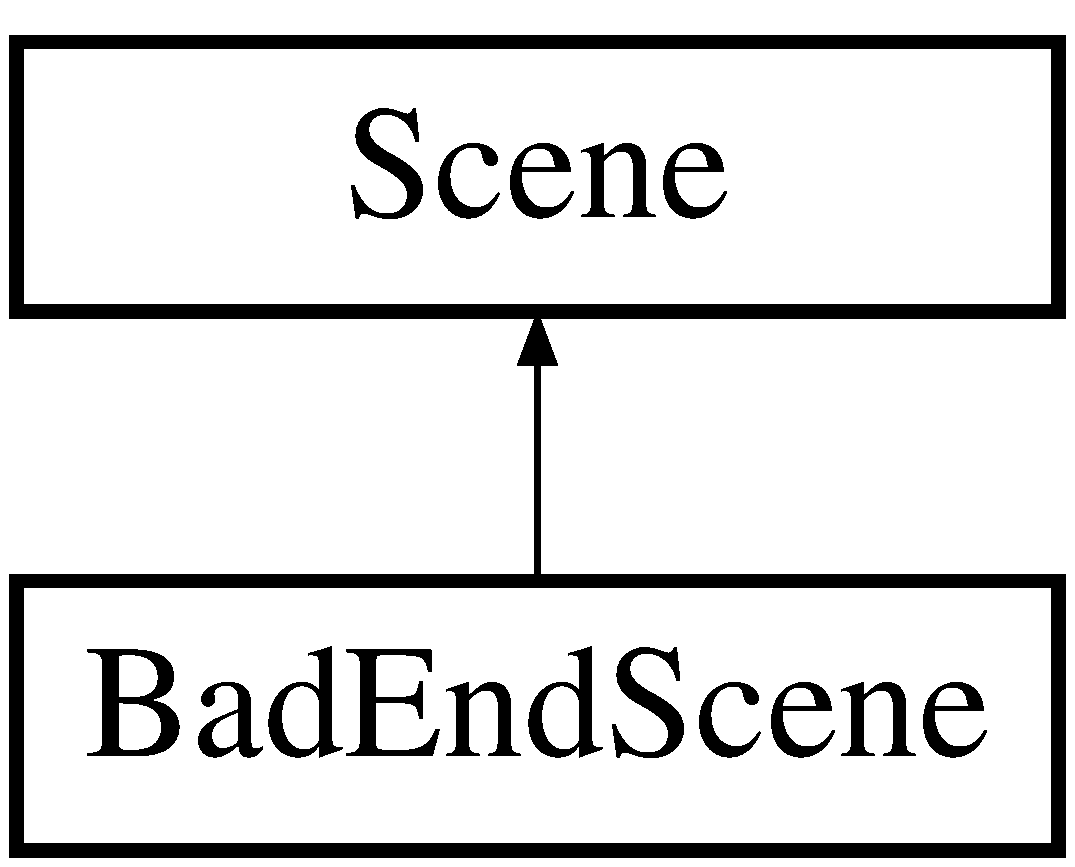
\includegraphics[height=2.000000cm]{class_bad_end_scene}
\end{center}
\end{figure}
\subsection*{\-Public 멤버 함수}
\begin{DoxyCompactItemize}
\item 
\hyperlink{class_bad_end_scene_a83568550e58e1c080cc5eb2c5be318a3}{\-Bad\-End\-Scene} ()
\item 
virtual void \hyperlink{class_bad_end_scene_a4d8802f274eaed7c1b28284505b2f8eb}{init} ()
\item 
virtual void \hyperlink{class_bad_end_scene_ae3dbd5c915a23f4c6ea47d57789a7545}{clean\-\_\-up} ()
\item 
virtual void \hyperlink{class_bad_end_scene_a8dd11870a1bc9115eaf2dd02a336c492}{do\-\_\-event} ()
\item 
virtual void \hyperlink{class_bad_end_scene_a668bb0f3c662a5698631adaf7f3a6829}{show} ()
\end{DoxyCompactItemize}


\subsection{생성자 \& 소멸자 문서화}
\hypertarget{class_bad_end_scene_a83568550e58e1c080cc5eb2c5be318a3}{\index{\-Bad\-End\-Scene@{\-Bad\-End\-Scene}!\-Bad\-End\-Scene@{\-Bad\-End\-Scene}}
\index{\-Bad\-End\-Scene@{\-Bad\-End\-Scene}!BadEndScene@{\-Bad\-End\-Scene}}
\subsubsection[{\-Bad\-End\-Scene}]{\setlength{\rightskip}{0pt plus 5cm}{\bf \-Bad\-End\-Scene\-::\-Bad\-End\-Scene} (
\begin{DoxyParamCaption}
{}
\end{DoxyParamCaption}
)}}\label{class_bad_end_scene_a83568550e58e1c080cc5eb2c5be318a3}


\subsection{멤버 함수 문서화}
\hypertarget{class_bad_end_scene_ae3dbd5c915a23f4c6ea47d57789a7545}{\index{\-Bad\-End\-Scene@{\-Bad\-End\-Scene}!clean\-\_\-up@{clean\-\_\-up}}
\index{clean\-\_\-up@{clean\-\_\-up}!BadEndScene@{\-Bad\-End\-Scene}}
\subsubsection[{clean\-\_\-up}]{\setlength{\rightskip}{0pt plus 5cm}void {\bf \-Bad\-End\-Scene\-::clean\-\_\-up} (
\begin{DoxyParamCaption}
{}
\end{DoxyParamCaption}
)\hspace{0.3cm}{\ttfamily  \mbox{[}virtual\mbox{]}}}}\label{class_bad_end_scene_ae3dbd5c915a23f4c6ea47d57789a7545}


\hyperlink{class_scene_a5f8c03499f5adff28224ccaaf95a8d90}{\-Scene}(으)로부터 재구현되었습니다.

\hypertarget{class_bad_end_scene_a8dd11870a1bc9115eaf2dd02a336c492}{\index{\-Bad\-End\-Scene@{\-Bad\-End\-Scene}!do\-\_\-event@{do\-\_\-event}}
\index{do\-\_\-event@{do\-\_\-event}!BadEndScene@{\-Bad\-End\-Scene}}
\subsubsection[{do\-\_\-event}]{\setlength{\rightskip}{0pt plus 5cm}void {\bf \-Bad\-End\-Scene\-::do\-\_\-event} (
\begin{DoxyParamCaption}
{}
\end{DoxyParamCaption}
)\hspace{0.3cm}{\ttfamily  \mbox{[}virtual\mbox{]}}}}\label{class_bad_end_scene_a8dd11870a1bc9115eaf2dd02a336c492}


\hyperlink{class_scene_a280970a0176e70f76d2420c50261d6fa}{\-Scene}(으)로부터 재구현되었습니다.

\hypertarget{class_bad_end_scene_a4d8802f274eaed7c1b28284505b2f8eb}{\index{\-Bad\-End\-Scene@{\-Bad\-End\-Scene}!init@{init}}
\index{init@{init}!BadEndScene@{\-Bad\-End\-Scene}}
\subsubsection[{init}]{\setlength{\rightskip}{0pt plus 5cm}void {\bf \-Bad\-End\-Scene\-::init} (
\begin{DoxyParamCaption}
{}
\end{DoxyParamCaption}
)\hspace{0.3cm}{\ttfamily  \mbox{[}virtual\mbox{]}}}}\label{class_bad_end_scene_a4d8802f274eaed7c1b28284505b2f8eb}


\hyperlink{class_scene_abb3b6efc6fdba03cd96436edaf08a967}{\-Scene}(으)로부터 재구현되었습니다.

\hypertarget{class_bad_end_scene_a668bb0f3c662a5698631adaf7f3a6829}{\index{\-Bad\-End\-Scene@{\-Bad\-End\-Scene}!show@{show}}
\index{show@{show}!BadEndScene@{\-Bad\-End\-Scene}}
\subsubsection[{show}]{\setlength{\rightskip}{0pt plus 5cm}void {\bf \-Bad\-End\-Scene\-::show} (
\begin{DoxyParamCaption}
{}
\end{DoxyParamCaption}
)\hspace{0.3cm}{\ttfamily  \mbox{[}virtual\mbox{]}}}}\label{class_bad_end_scene_a668bb0f3c662a5698631adaf7f3a6829}


\hyperlink{class_scene_a6f447a90b1f9009acfb72df711473875}{\-Scene}(으)로부터 재구현되었습니다.



이 클래스에 대한 문서화 페이지는 다음의 파일들로부터 생성되었습니다.\-:\begin{DoxyCompactItemize}
\item 
\hyperlink{_scene_8h}{\-Scene.\-h}\item 
\hyperlink{_scene_8cpp}{\-Scene.\-cpp}\end{DoxyCompactItemize}

\hypertarget{class_building}{\section{\-Building 클래스 참조}
\label{class_building}\index{\-Building@{\-Building}}
}


{\ttfamily \#include $<$building.\-h$>$}

\-Building에 대한 상속 다이어그램 \-: \begin{figure}[H]
\begin{center}
\leavevmode
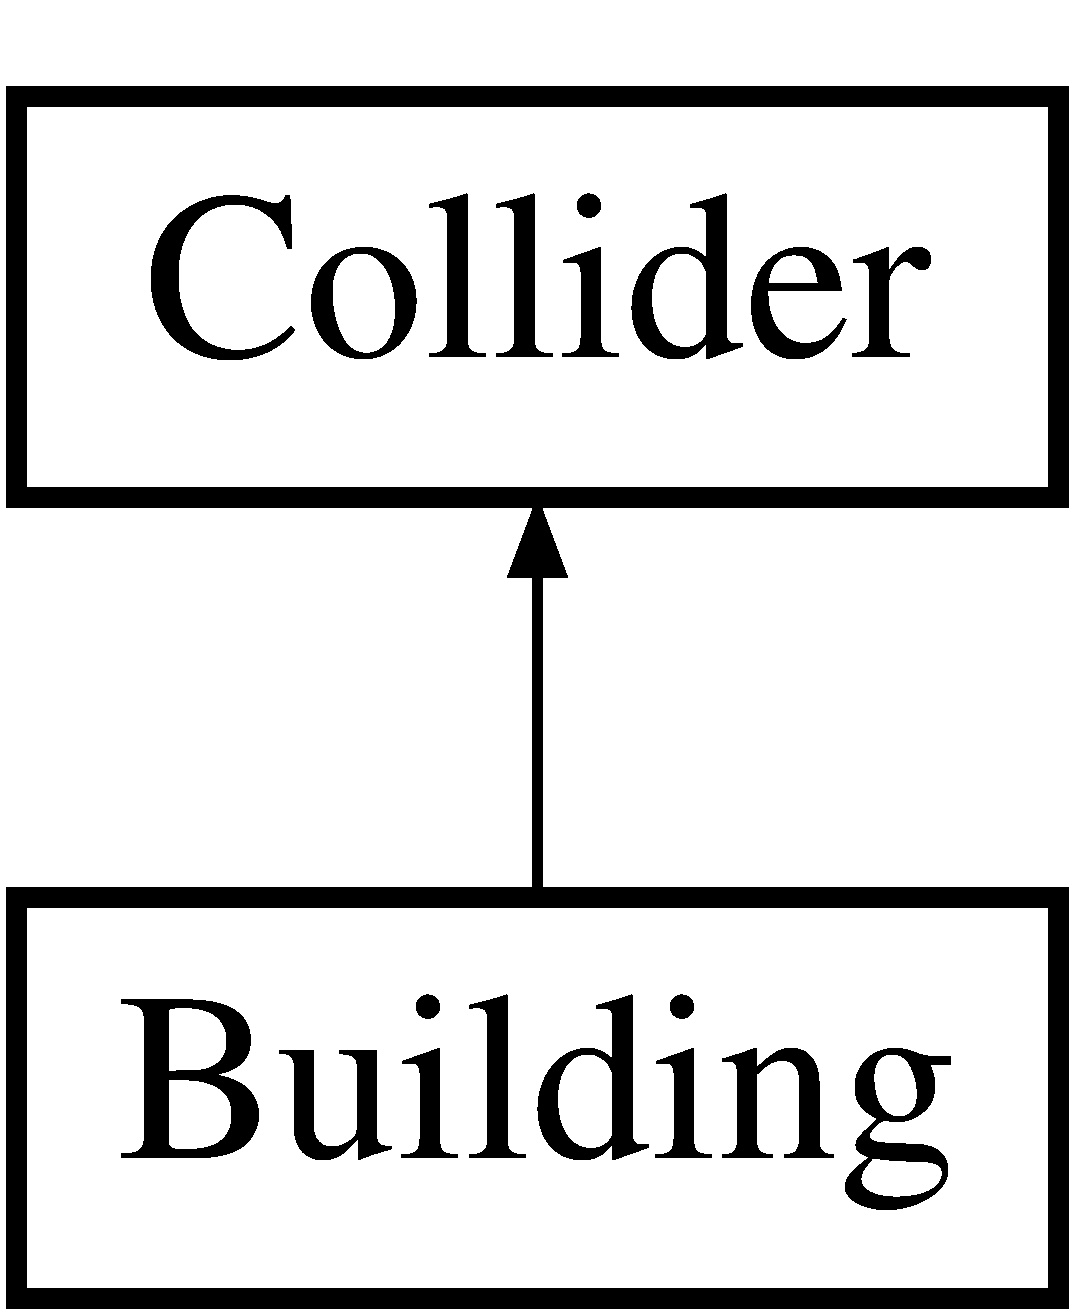
\includegraphics[height=2.000000cm]{class_building}
\end{center}
\end{figure}
\subsection*{\-Public 멤버 함수}
\begin{DoxyCompactItemize}
\item 
\hyperlink{class_building_a3196128a859083cc124e4e783f2abfe2}{\-Building} (int \-\_\-x, int \-\_\-y, int \-\_\-w, int \-\_\-h)
\item 
void \hyperlink{class_building_ada54cf04765575df590b78a7df573395}{init} (\hyperlink{_constants_8h_a03f7ec9e12b891db1bbeda07eb4099d7}{\-E\-Card} p\-Card)
\item 
virtual bool \hyperlink{class_building_a02c1ac48410c20319a30e6ce13433212}{check\-\_\-collide} (\hyperlink{class_collider}{\-Collider} $\ast$)
\item 
virtual \-S\-D\-L\-\_\-\-Rect $\ast$ \hyperlink{class_building_abb1a4ea20e451db134810c45d530e19f}{get\-\_\-box} ()
\item 
void \hyperlink{class_building_adb755e094e0017cc0834dbaa81f08888}{clean\-\_\-up} ()
\item 
void \hyperlink{class_building_a4cb46a187a9c0d9d4bb68c5e8d8a801a}{show} ()
\item 
\hyperlink{class_door}{\-Door} $\ast$ \hyperlink{class_building_a422d693cd9f6ba552a7abba9c0f7f22b}{get\-\_\-door} ()
\end{DoxyCompactItemize}
\subsection*{\-Public 속성}
\begin{DoxyCompactItemize}
\item 
int \hyperlink{class_building_a853be442e19c87017130550963def9ff}{card\-\_\-id}
\end{DoxyCompactItemize}


\subsection{생성자 \& 소멸자 문서화}
\hypertarget{class_building_a3196128a859083cc124e4e783f2abfe2}{\index{\-Building@{\-Building}!\-Building@{\-Building}}
\index{\-Building@{\-Building}!Building@{\-Building}}
\subsubsection[{\-Building}]{\setlength{\rightskip}{0pt plus 5cm}{\bf \-Building\-::\-Building} (
\begin{DoxyParamCaption}
\item[{int}]{\-\_\-x, }
\item[{int}]{\-\_\-y, }
\item[{int}]{\-\_\-w, }
\item[{int}]{\-\_\-h}
\end{DoxyParamCaption}
)}}\label{class_building_a3196128a859083cc124e4e783f2abfe2}


\subsection{멤버 함수 문서화}
\hypertarget{class_building_a02c1ac48410c20319a30e6ce13433212}{\index{\-Building@{\-Building}!check\-\_\-collide@{check\-\_\-collide}}
\index{check\-\_\-collide@{check\-\_\-collide}!Building@{\-Building}}
\subsubsection[{check\-\_\-collide}]{\setlength{\rightskip}{0pt plus 5cm}bool {\bf \-Building\-::check\-\_\-collide} (
\begin{DoxyParamCaption}
\item[{{\bf \-Collider} $\ast$}]{other}
\end{DoxyParamCaption}
)\hspace{0.3cm}{\ttfamily  \mbox{[}virtual\mbox{]}}}}\label{class_building_a02c1ac48410c20319a30e6ce13433212}


\hyperlink{class_collider_aa14301229ec52e3219b41c17ef162925}{\-Collider}를 구현.

\hypertarget{class_building_adb755e094e0017cc0834dbaa81f08888}{\index{\-Building@{\-Building}!clean\-\_\-up@{clean\-\_\-up}}
\index{clean\-\_\-up@{clean\-\_\-up}!Building@{\-Building}}
\subsubsection[{clean\-\_\-up}]{\setlength{\rightskip}{0pt plus 5cm}void {\bf \-Building\-::clean\-\_\-up} (
\begin{DoxyParamCaption}
{}
\end{DoxyParamCaption}
)}}\label{class_building_adb755e094e0017cc0834dbaa81f08888}
\hypertarget{class_building_abb1a4ea20e451db134810c45d530e19f}{\index{\-Building@{\-Building}!get\-\_\-box@{get\-\_\-box}}
\index{get\-\_\-box@{get\-\_\-box}!Building@{\-Building}}
\subsubsection[{get\-\_\-box}]{\setlength{\rightskip}{0pt plus 5cm}\-S\-D\-L\-\_\-\-Rect $\ast$ {\bf \-Building\-::get\-\_\-box} (
\begin{DoxyParamCaption}
{}
\end{DoxyParamCaption}
)\hspace{0.3cm}{\ttfamily  \mbox{[}virtual\mbox{]}}}}\label{class_building_abb1a4ea20e451db134810c45d530e19f}


\hyperlink{class_collider_a1b6c8bc800070a1e880979378b348e8d}{\-Collider}를 구현.

\hypertarget{class_building_a422d693cd9f6ba552a7abba9c0f7f22b}{\index{\-Building@{\-Building}!get\-\_\-door@{get\-\_\-door}}
\index{get\-\_\-door@{get\-\_\-door}!Building@{\-Building}}
\subsubsection[{get\-\_\-door}]{\setlength{\rightskip}{0pt plus 5cm}{\bf \-Door} $\ast$ {\bf \-Building\-::get\-\_\-door} (
\begin{DoxyParamCaption}
{}
\end{DoxyParamCaption}
)}}\label{class_building_a422d693cd9f6ba552a7abba9c0f7f22b}
\hypertarget{class_building_ada54cf04765575df590b78a7df573395}{\index{\-Building@{\-Building}!init@{init}}
\index{init@{init}!Building@{\-Building}}
\subsubsection[{init}]{\setlength{\rightskip}{0pt plus 5cm}void {\bf \-Building\-::init} (
\begin{DoxyParamCaption}
\item[{{\bf \-E\-Card}}]{p\-Card}
\end{DoxyParamCaption}
)}}\label{class_building_ada54cf04765575df590b78a7df573395}
\hypertarget{class_building_a4cb46a187a9c0d9d4bb68c5e8d8a801a}{\index{\-Building@{\-Building}!show@{show}}
\index{show@{show}!Building@{\-Building}}
\subsubsection[{show}]{\setlength{\rightskip}{0pt plus 5cm}void {\bf \-Building\-::show} (
\begin{DoxyParamCaption}
{}
\end{DoxyParamCaption}
)}}\label{class_building_a4cb46a187a9c0d9d4bb68c5e8d8a801a}


\subsection{멤버 데이타 문서화}
\hypertarget{class_building_a853be442e19c87017130550963def9ff}{\index{\-Building@{\-Building}!card\-\_\-id@{card\-\_\-id}}
\index{card\-\_\-id@{card\-\_\-id}!Building@{\-Building}}
\subsubsection[{card\-\_\-id}]{\setlength{\rightskip}{0pt plus 5cm}int {\bf \-Building\-::card\-\_\-id}}}\label{class_building_a853be442e19c87017130550963def9ff}


이 클래스에 대한 문서화 페이지는 다음의 파일들로부터 생성되었습니다.\-:\begin{DoxyCompactItemize}
\item 
\hyperlink{building_8h}{building.\-h}\item 
\hyperlink{building_8cpp}{building.\-cpp}\end{DoxyCompactItemize}

\hypertarget{class_card}{\section{\-Card 클래스 참조}
\label{class_card}\index{\-Card@{\-Card}}
}


{\ttfamily \#include $<$\-Card.\-h$>$}

\subsection*{\-Public 멤버 함수}
\begin{DoxyCompactItemize}
\item 
\hyperlink{class_card_ac92bc3e9ac6d70ca67af2bb778a6cccb}{\-Card} (int credit\-\_\-limit, int gage)
\item 
std\-::string \hyperlink{class_card_a895bb063f4337b6fe047c43f63c0470f}{print} ()
\end{DoxyCompactItemize}


\subsection{생성자 \& 소멸자 문서화}
\hypertarget{class_card_ac92bc3e9ac6d70ca67af2bb778a6cccb}{\index{\-Card@{\-Card}!\-Card@{\-Card}}
\index{\-Card@{\-Card}!Card@{\-Card}}
\subsubsection[{\-Card}]{\setlength{\rightskip}{0pt plus 5cm}{\bf \-Card\-::\-Card} (
\begin{DoxyParamCaption}
\item[{int}]{credit\-\_\-limit, }
\item[{int}]{gage}
\end{DoxyParamCaption}
)}}\label{class_card_ac92bc3e9ac6d70ca67af2bb778a6cccb}


\subsection{멤버 함수 문서화}
\hypertarget{class_card_a895bb063f4337b6fe047c43f63c0470f}{\index{\-Card@{\-Card}!print@{print}}
\index{print@{print}!Card@{\-Card}}
\subsubsection[{print}]{\setlength{\rightskip}{0pt plus 5cm}std\-::string {\bf \-Card\-::print} (
\begin{DoxyParamCaption}
{}
\end{DoxyParamCaption}
)}}\label{class_card_a895bb063f4337b6fe047c43f63c0470f}


이 클래스에 대한 문서화 페이지는 다음의 파일들로부터 생성되었습니다.\-:\begin{DoxyCompactItemize}
\item 
\hyperlink{_card_8h}{\-Card.\-h}\item 
\hyperlink{_card_8cpp}{\-Card.\-cpp}\end{DoxyCompactItemize}

\hypertarget{class_c_card}{\section{\-C\-Card 클래스 참조}
\label{class_c_card}\index{\-C\-Card@{\-C\-Card}}
}


{\ttfamily \#include $<$\-C\-Card.\-h$>$}

\subsection*{\-Public 멤버 함수}
\begin{DoxyCompactItemize}
\item 
\hyperlink{class_c_card_aa4dcdbe0d0ec085e0b389af7324e9486}{\-C\-Card} ()
\item 
void \hyperlink{class_c_card_a9a38050657972e24f78946c3cd00f8ea}{\-Reset} ()
\item 
void \hyperlink{class_c_card_abca7c4b70ec5c5bc576cd8aae4249c8e}{\-Set\-Card} (int p\-Card\-No)
\item 
void \hyperlink{class_c_card_a7f3e715065d6a12c783800be7d6a2c37}{\-Set\-Gage} (int p\-Gage)
\item 
void \hyperlink{class_c_card_aa8c7fc4dc97f1c75b1f5fba01184faf4}{\-Plus\-Gage} (int p\-Add)
\item 
void \hyperlink{class_c_card_ad1856729f625e4471cf9a53b532d4ccc}{\-Minus\-Gage} (int p\-Minus)
\item 
bool \hyperlink{class_c_card_a7d70a6c3bd33c10d91798406bdea9a6b}{\-Set\-Dept} (uint64\-\_\-t p\-Dept)
\item 
bool \hyperlink{class_c_card_a2610e5a55aefb4218c619c1d4d349883}{\-Buy\-Something} (uint64\-\_\-t p\-Price)
\item 
bool \hyperlink{class_c_card_a2fbb6cdc260f3835e4551c50e66daae4}{\-Add\-Dept} (uint64\-\_\-t p\-Money)
\item 
void \hyperlink{class_c_card_adb058ac448af3e5a4e7f15cf9c7037df}{\-Set\-Limit} (unsigned short p\-Grade, \hyperlink{_constants_8h_a4db5fb2e90acc4ef6c281d6cca4dea4e}{\-E\-Rank} p\-Rank)
\item 
int \hyperlink{class_c_card_ad129e69c37d03413300a6b6870625656}{\-Get\-Card\-No} (void) const 
\item 
int \hyperlink{class_c_card_ab9e6eca765f088ba12692c5a59720320}{\-Get\-Gage} (void) const 
\item 
uint64\-\_\-t \hyperlink{class_c_card_a7db6358703921c625c1d2a79418dfb9c}{\-Get\-Dept} (void) const 
\item 
uint64\-\_\-t \hyperlink{class_c_card_aecf5a0ace3aa06dcc043dd17c0884d34}{\-Get\-Limit} (void) const 
\end{DoxyCompactItemize}


\subsection{생성자 \& 소멸자 문서화}
\hypertarget{class_c_card_aa4dcdbe0d0ec085e0b389af7324e9486}{\index{\-C\-Card@{\-C\-Card}!\-C\-Card@{\-C\-Card}}
\index{\-C\-Card@{\-C\-Card}!CCard@{\-C\-Card}}
\subsubsection[{\-C\-Card}]{\setlength{\rightskip}{0pt plus 5cm}{\bf \-C\-Card\-::\-C\-Card} (
\begin{DoxyParamCaption}
{}
\end{DoxyParamCaption}
)}}\label{class_c_card_aa4dcdbe0d0ec085e0b389af7324e9486}


\subsection{멤버 함수 문서화}
\hypertarget{class_c_card_a2fbb6cdc260f3835e4551c50e66daae4}{\index{\-C\-Card@{\-C\-Card}!\-Add\-Dept@{\-Add\-Dept}}
\index{\-Add\-Dept@{\-Add\-Dept}!CCard@{\-C\-Card}}
\subsubsection[{\-Add\-Dept}]{\setlength{\rightskip}{0pt plus 5cm}bool {\bf \-C\-Card\-::\-Add\-Dept} (
\begin{DoxyParamCaption}
\item[{uint64\-\_\-t}]{p\-Money}
\end{DoxyParamCaption}
)}}\label{class_c_card_a2fbb6cdc260f3835e4551c50e66daae4}
\hypertarget{class_c_card_a2610e5a55aefb4218c619c1d4d349883}{\index{\-C\-Card@{\-C\-Card}!\-Buy\-Something@{\-Buy\-Something}}
\index{\-Buy\-Something@{\-Buy\-Something}!CCard@{\-C\-Card}}
\subsubsection[{\-Buy\-Something}]{\setlength{\rightskip}{0pt plus 5cm}bool {\bf \-C\-Card\-::\-Buy\-Something} (
\begin{DoxyParamCaption}
\item[{uint64\-\_\-t}]{p\-Price}
\end{DoxyParamCaption}
)}}\label{class_c_card_a2610e5a55aefb4218c619c1d4d349883}
\hypertarget{class_c_card_ad129e69c37d03413300a6b6870625656}{\index{\-C\-Card@{\-C\-Card}!\-Get\-Card\-No@{\-Get\-Card\-No}}
\index{\-Get\-Card\-No@{\-Get\-Card\-No}!CCard@{\-C\-Card}}
\subsubsection[{\-Get\-Card\-No}]{\setlength{\rightskip}{0pt plus 5cm}int {\bf \-C\-Card\-::\-Get\-Card\-No} (
\begin{DoxyParamCaption}
\item[{void}]{}
\end{DoxyParamCaption}
) const}}\label{class_c_card_ad129e69c37d03413300a6b6870625656}
\hypertarget{class_c_card_a7db6358703921c625c1d2a79418dfb9c}{\index{\-C\-Card@{\-C\-Card}!\-Get\-Dept@{\-Get\-Dept}}
\index{\-Get\-Dept@{\-Get\-Dept}!CCard@{\-C\-Card}}
\subsubsection[{\-Get\-Dept}]{\setlength{\rightskip}{0pt plus 5cm}uint64\-\_\-t {\bf \-C\-Card\-::\-Get\-Dept} (
\begin{DoxyParamCaption}
\item[{void}]{}
\end{DoxyParamCaption}
) const}}\label{class_c_card_a7db6358703921c625c1d2a79418dfb9c}
\hypertarget{class_c_card_ab9e6eca765f088ba12692c5a59720320}{\index{\-C\-Card@{\-C\-Card}!\-Get\-Gage@{\-Get\-Gage}}
\index{\-Get\-Gage@{\-Get\-Gage}!CCard@{\-C\-Card}}
\subsubsection[{\-Get\-Gage}]{\setlength{\rightskip}{0pt plus 5cm}int {\bf \-C\-Card\-::\-Get\-Gage} (
\begin{DoxyParamCaption}
\item[{void}]{}
\end{DoxyParamCaption}
) const}}\label{class_c_card_ab9e6eca765f088ba12692c5a59720320}
\hypertarget{class_c_card_aecf5a0ace3aa06dcc043dd17c0884d34}{\index{\-C\-Card@{\-C\-Card}!\-Get\-Limit@{\-Get\-Limit}}
\index{\-Get\-Limit@{\-Get\-Limit}!CCard@{\-C\-Card}}
\subsubsection[{\-Get\-Limit}]{\setlength{\rightskip}{0pt plus 5cm}uint64\-\_\-t {\bf \-C\-Card\-::\-Get\-Limit} (
\begin{DoxyParamCaption}
\item[{void}]{}
\end{DoxyParamCaption}
) const}}\label{class_c_card_aecf5a0ace3aa06dcc043dd17c0884d34}
\hypertarget{class_c_card_ad1856729f625e4471cf9a53b532d4ccc}{\index{\-C\-Card@{\-C\-Card}!\-Minus\-Gage@{\-Minus\-Gage}}
\index{\-Minus\-Gage@{\-Minus\-Gage}!CCard@{\-C\-Card}}
\subsubsection[{\-Minus\-Gage}]{\setlength{\rightskip}{0pt plus 5cm}void {\bf \-C\-Card\-::\-Minus\-Gage} (
\begin{DoxyParamCaption}
\item[{int}]{p\-Minus}
\end{DoxyParamCaption}
)}}\label{class_c_card_ad1856729f625e4471cf9a53b532d4ccc}
\hypertarget{class_c_card_aa8c7fc4dc97f1c75b1f5fba01184faf4}{\index{\-C\-Card@{\-C\-Card}!\-Plus\-Gage@{\-Plus\-Gage}}
\index{\-Plus\-Gage@{\-Plus\-Gage}!CCard@{\-C\-Card}}
\subsubsection[{\-Plus\-Gage}]{\setlength{\rightskip}{0pt plus 5cm}void {\bf \-C\-Card\-::\-Plus\-Gage} (
\begin{DoxyParamCaption}
\item[{int}]{p\-Add}
\end{DoxyParamCaption}
)}}\label{class_c_card_aa8c7fc4dc97f1c75b1f5fba01184faf4}
\hypertarget{class_c_card_a9a38050657972e24f78946c3cd00f8ea}{\index{\-C\-Card@{\-C\-Card}!\-Reset@{\-Reset}}
\index{\-Reset@{\-Reset}!CCard@{\-C\-Card}}
\subsubsection[{\-Reset}]{\setlength{\rightskip}{0pt plus 5cm}void {\bf \-C\-Card\-::\-Reset} (
\begin{DoxyParamCaption}
\item[{void}]{}
\end{DoxyParamCaption}
)}}\label{class_c_card_a9a38050657972e24f78946c3cd00f8ea}
\hypertarget{class_c_card_abca7c4b70ec5c5bc576cd8aae4249c8e}{\index{\-C\-Card@{\-C\-Card}!\-Set\-Card@{\-Set\-Card}}
\index{\-Set\-Card@{\-Set\-Card}!CCard@{\-C\-Card}}
\subsubsection[{\-Set\-Card}]{\setlength{\rightskip}{0pt plus 5cm}void {\bf \-C\-Card\-::\-Set\-Card} (
\begin{DoxyParamCaption}
\item[{int}]{p\-Card\-No}
\end{DoxyParamCaption}
)}}\label{class_c_card_abca7c4b70ec5c5bc576cd8aae4249c8e}
\hypertarget{class_c_card_a7d70a6c3bd33c10d91798406bdea9a6b}{\index{\-C\-Card@{\-C\-Card}!\-Set\-Dept@{\-Set\-Dept}}
\index{\-Set\-Dept@{\-Set\-Dept}!CCard@{\-C\-Card}}
\subsubsection[{\-Set\-Dept}]{\setlength{\rightskip}{0pt plus 5cm}bool {\bf \-C\-Card\-::\-Set\-Dept} (
\begin{DoxyParamCaption}
\item[{uint64\-\_\-t}]{p\-Dept}
\end{DoxyParamCaption}
)}}\label{class_c_card_a7d70a6c3bd33c10d91798406bdea9a6b}
\hypertarget{class_c_card_a7f3e715065d6a12c783800be7d6a2c37}{\index{\-C\-Card@{\-C\-Card}!\-Set\-Gage@{\-Set\-Gage}}
\index{\-Set\-Gage@{\-Set\-Gage}!CCard@{\-C\-Card}}
\subsubsection[{\-Set\-Gage}]{\setlength{\rightskip}{0pt plus 5cm}void {\bf \-C\-Card\-::\-Set\-Gage} (
\begin{DoxyParamCaption}
\item[{int}]{p\-Gage}
\end{DoxyParamCaption}
)}}\label{class_c_card_a7f3e715065d6a12c783800be7d6a2c37}
\hypertarget{class_c_card_adb058ac448af3e5a4e7f15cf9c7037df}{\index{\-C\-Card@{\-C\-Card}!\-Set\-Limit@{\-Set\-Limit}}
\index{\-Set\-Limit@{\-Set\-Limit}!CCard@{\-C\-Card}}
\subsubsection[{\-Set\-Limit}]{\setlength{\rightskip}{0pt plus 5cm}void {\bf \-C\-Card\-::\-Set\-Limit} (
\begin{DoxyParamCaption}
\item[{unsigned short}]{p\-Grade, }
\item[{{\bf \-E\-Rank}}]{p\-Rank}
\end{DoxyParamCaption}
)}}\label{class_c_card_adb058ac448af3e5a4e7f15cf9c7037df}


이 클래스에 대한 문서화 페이지는 다음의 파일들로부터 생성되었습니다.\-:\begin{DoxyCompactItemize}
\item 
\hyperlink{_c_card_8h}{\-C\-Card.\-h}\item 
\hyperlink{_c_card_8cpp}{\-C\-Card.\-cpp}\end{DoxyCompactItemize}

\hypertarget{class_character}{\section{\-Character 클래스 참조}
\label{class_character}\index{\-Character@{\-Character}}
}


{\ttfamily \#include $<$character.\-h$>$}

\-Character에 대한 상속 다이어그램 \-: \begin{figure}[H]
\begin{center}
\leavevmode
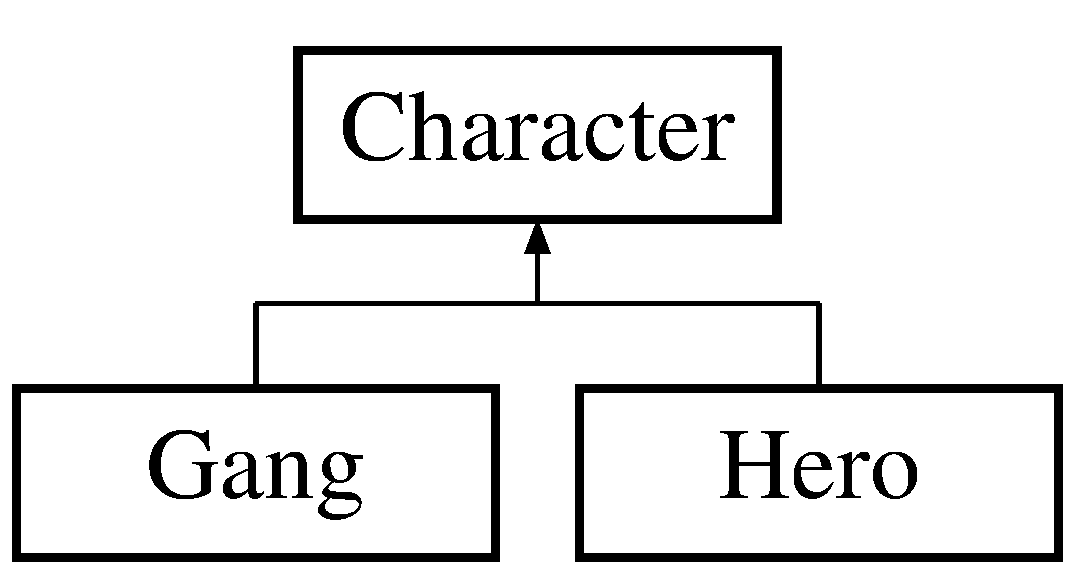
\includegraphics[height=2.000000cm]{class_character}
\end{center}
\end{figure}
\subsection*{\-Public 멤버 함수}
\begin{DoxyCompactItemize}
\item 
virtual \hyperlink{class_character_a9e9be564d05ded80962b2045aa70b3fc}{$\sim$\-Character} ()
\item 
virtual bool \hyperlink{class_character_a32f64bd79aac4bcdfa3878b34ffd39da}{move} (\-Uint32 delta\-Ticks)
\item 
virtual void \hyperlink{class_character_ae026a3baf7b9a31c270b9b0596c5e181}{init} ()
\item 
virtual void \hyperlink{class_character_a2304027ce7b4caf5a1851e371f3071cd}{clean\-\_\-up} ()
\item 
virtual void \hyperlink{class_character_aee8d4cab5de7363e08ebcaf14171a454}{show} (\-S\-D\-L\-\_\-\-Surface $\ast$)
\item 
virtual void \hyperlink{class_character_ae29d39664b615ddee1fd855569cade90}{set\-\_\-clip} ()
\item 
virtual void \hyperlink{class_character_a074348cfffee21b386e6ed3d950a7f2f}{add\-\_\-person} ()
\item 
virtual void \hyperlink{class_character_a24e66bb11b377efa0079393d6ed99e89}{set\-\_\-object} (\-S\-D\-L\-\_\-\-Rect $\ast$object)
\item 
virtual void \hyperlink{class_character_a33e738893b424f6e890f49d756c7ffe6}{move\-\_\-back} ()
\end{DoxyCompactItemize}
\subsection*{\-Protected 속성}
\begin{DoxyCompactItemize}
\item 
int \hyperlink{class_character_a03d37d245f17ffb4302f8b37141390bb}{x}
\item 
int \hyperlink{class_character_a3b64a782ef7f82581760ccaf68521be3}{y}
\item 
int \hyperlink{class_character_ac3c6fdfe5ccb5e984c83e20c28e7e4f2}{p\-\_\-x}
\item 
int \hyperlink{class_character_a9d10eb04b9cb779d432707f34171fb79}{p\-\_\-y}
\item 
int \hyperlink{class_character_adf848d11acd46785ec3408a018b4dabe}{w}
\item 
int \hyperlink{class_character_a5a455718929221529a9c01781579927b}{h}
\item 
int \hyperlink{class_character_a769c5656e887d69472f08f9de9589eb5}{x\-Vel}
\item 
int \hyperlink{class_character_aba005243607dd2e77f798e70675af9f5}{y\-Vel}
\item 
\-S\-D\-L\-\_\-\-Surface $\ast$ \hyperlink{class_character_a1769b630de33a3da0dd7456e71350a84}{image}
\item 
int \hyperlink{class_character_a78ea8d15292e89650d12d98878bac42c}{frame}
\item 
\-S\-D\-L\-\_\-\-Rect \hyperlink{class_character_a597a53af58019f1654e70714bacab249}{clip} \mbox{[}4\mbox{]}\mbox{[}3\mbox{]}
\end{DoxyCompactItemize}


\subsection{생성자 \& 소멸자 문서화}
\hypertarget{class_character_a9e9be564d05ded80962b2045aa70b3fc}{\index{\-Character@{\-Character}!$\sim$\-Character@{$\sim$\-Character}}
\index{$\sim$\-Character@{$\sim$\-Character}!Character@{\-Character}}
\subsubsection[{$\sim$\-Character}]{\setlength{\rightskip}{0pt plus 5cm}{\bf \-Character\-::$\sim$\-Character} (
\begin{DoxyParamCaption}
{}
\end{DoxyParamCaption}
)\hspace{0.3cm}{\ttfamily  \mbox{[}virtual\mbox{]}}}}\label{class_character_a9e9be564d05ded80962b2045aa70b3fc}


\subsection{멤버 함수 문서화}
\hypertarget{class_character_a074348cfffee21b386e6ed3d950a7f2f}{\index{\-Character@{\-Character}!add\-\_\-person@{add\-\_\-person}}
\index{add\-\_\-person@{add\-\_\-person}!Character@{\-Character}}
\subsubsection[{add\-\_\-person}]{\setlength{\rightskip}{0pt plus 5cm}void {\bf \-Character\-::add\-\_\-person} (
\begin{DoxyParamCaption}
{}
\end{DoxyParamCaption}
)\hspace{0.3cm}{\ttfamily  \mbox{[}virtual\mbox{]}}}}\label{class_character_a074348cfffee21b386e6ed3d950a7f2f}


\hyperlink{class_gang_ad177257ab75d22c409b6b7b89c5d0870}{\-Gang}, \hyperlink{class_hero_aa8934d60bc26f9eefdc15661d924e5e0}{\-Hero}에서 재구현되었습니다.

\hypertarget{class_character_a2304027ce7b4caf5a1851e371f3071cd}{\index{\-Character@{\-Character}!clean\-\_\-up@{clean\-\_\-up}}
\index{clean\-\_\-up@{clean\-\_\-up}!Character@{\-Character}}
\subsubsection[{clean\-\_\-up}]{\setlength{\rightskip}{0pt plus 5cm}void {\bf \-Character\-::clean\-\_\-up} (
\begin{DoxyParamCaption}
{}
\end{DoxyParamCaption}
)\hspace{0.3cm}{\ttfamily  \mbox{[}virtual\mbox{]}}}}\label{class_character_a2304027ce7b4caf5a1851e371f3071cd}


\hyperlink{class_gang_af472124b9a8c3e4a5950562342ec8162}{\-Gang}, \hyperlink{class_hero_a43836f7e926f00a4a27757a1ff7410a0}{\-Hero}에서 재구현되었습니다.

\hypertarget{class_character_ae026a3baf7b9a31c270b9b0596c5e181}{\index{\-Character@{\-Character}!init@{init}}
\index{init@{init}!Character@{\-Character}}
\subsubsection[{init}]{\setlength{\rightskip}{0pt plus 5cm}void {\bf \-Character\-::init} (
\begin{DoxyParamCaption}
{}
\end{DoxyParamCaption}
)\hspace{0.3cm}{\ttfamily  \mbox{[}virtual\mbox{]}}}}\label{class_character_ae026a3baf7b9a31c270b9b0596c5e181}


\hyperlink{class_gang_a3788b8ace6c57cdcdc464a2f96169484}{\-Gang}, \hyperlink{class_hero_ae67cc4b7770083755895b78664d0ea34}{\-Hero}에서 재구현되었습니다.

\hypertarget{class_character_a32f64bd79aac4bcdfa3878b34ffd39da}{\index{\-Character@{\-Character}!move@{move}}
\index{move@{move}!Character@{\-Character}}
\subsubsection[{move}]{\setlength{\rightskip}{0pt plus 5cm}bool {\bf \-Character\-::move} (
\begin{DoxyParamCaption}
\item[{\-Uint32}]{delta\-Ticks}
\end{DoxyParamCaption}
)\hspace{0.3cm}{\ttfamily  \mbox{[}virtual\mbox{]}}}}\label{class_character_a32f64bd79aac4bcdfa3878b34ffd39da}


\hyperlink{class_gang_abccb863ee9ef936fad5031a0d93e1b55}{\-Gang}, \hyperlink{class_hero_a0961b6b66165095e3d764ccc60436846}{\-Hero}에서 재구현되었습니다.

\hypertarget{class_character_a33e738893b424f6e890f49d756c7ffe6}{\index{\-Character@{\-Character}!move\-\_\-back@{move\-\_\-back}}
\index{move\-\_\-back@{move\-\_\-back}!Character@{\-Character}}
\subsubsection[{move\-\_\-back}]{\setlength{\rightskip}{0pt plus 5cm}void {\bf \-Character\-::move\-\_\-back} (
\begin{DoxyParamCaption}
{}
\end{DoxyParamCaption}
)\hspace{0.3cm}{\ttfamily  \mbox{[}virtual\mbox{]}}}}\label{class_character_a33e738893b424f6e890f49d756c7ffe6}


\hyperlink{class_gang_ac3aa2c0e70ecf1e7ce42192f684d1398}{\-Gang}, \hyperlink{class_hero_a805934d28498398aecb10f8d2de6b63e}{\-Hero}에서 재구현되었습니다.

\hypertarget{class_character_ae29d39664b615ddee1fd855569cade90}{\index{\-Character@{\-Character}!set\-\_\-clip@{set\-\_\-clip}}
\index{set\-\_\-clip@{set\-\_\-clip}!Character@{\-Character}}
\subsubsection[{set\-\_\-clip}]{\setlength{\rightskip}{0pt plus 5cm}void {\bf \-Character\-::set\-\_\-clip} (
\begin{DoxyParamCaption}
{}
\end{DoxyParamCaption}
)\hspace{0.3cm}{\ttfamily  \mbox{[}virtual\mbox{]}}}}\label{class_character_ae29d39664b615ddee1fd855569cade90}


\hyperlink{class_gang_af4463fb95507a172b1495fae411bfba5}{\-Gang}, \hyperlink{class_hero_aa5bde5d2f4a3d086b9e8ce2b969e2f3f}{\-Hero}에서 재구현되었습니다.

\hypertarget{class_character_a24e66bb11b377efa0079393d6ed99e89}{\index{\-Character@{\-Character}!set\-\_\-object@{set\-\_\-object}}
\index{set\-\_\-object@{set\-\_\-object}!Character@{\-Character}}
\subsubsection[{set\-\_\-object}]{\setlength{\rightskip}{0pt plus 5cm}void {\bf \-Character\-::set\-\_\-object} (
\begin{DoxyParamCaption}
\item[{\-S\-D\-L\-\_\-\-Rect $\ast$}]{object}
\end{DoxyParamCaption}
)\hspace{0.3cm}{\ttfamily  \mbox{[}virtual\mbox{]}}}}\label{class_character_a24e66bb11b377efa0079393d6ed99e89}


\hyperlink{class_gang_a74c369149d11573fbad437d997266c36}{\-Gang}에서 재구현되었습니다.

\hypertarget{class_character_aee8d4cab5de7363e08ebcaf14171a454}{\index{\-Character@{\-Character}!show@{show}}
\index{show@{show}!Character@{\-Character}}
\subsubsection[{show}]{\setlength{\rightskip}{0pt plus 5cm}void {\bf \-Character\-::show} (
\begin{DoxyParamCaption}
\item[{\-S\-D\-L\-\_\-\-Surface $\ast$}]{}
\end{DoxyParamCaption}
)\hspace{0.3cm}{\ttfamily  \mbox{[}virtual\mbox{]}}}}\label{class_character_aee8d4cab5de7363e08ebcaf14171a454}


\hyperlink{class_gang_a29330bf2df1bd60644513b2cb27f29e6}{\-Gang}, \hyperlink{class_hero_a9670c2232f5bf0f66bba60a7c747c53d}{\-Hero}에서 재구현되었습니다.



\subsection{멤버 데이타 문서화}
\hypertarget{class_character_a597a53af58019f1654e70714bacab249}{\index{\-Character@{\-Character}!clip@{clip}}
\index{clip@{clip}!Character@{\-Character}}
\subsubsection[{clip}]{\setlength{\rightskip}{0pt plus 5cm}\-S\-D\-L\-\_\-\-Rect {\bf \-Character\-::clip}\mbox{[}4\mbox{]}\mbox{[}3\mbox{]}\hspace{0.3cm}{\ttfamily  \mbox{[}protected\mbox{]}}}}\label{class_character_a597a53af58019f1654e70714bacab249}
\hypertarget{class_character_a78ea8d15292e89650d12d98878bac42c}{\index{\-Character@{\-Character}!frame@{frame}}
\index{frame@{frame}!Character@{\-Character}}
\subsubsection[{frame}]{\setlength{\rightskip}{0pt plus 5cm}int {\bf \-Character\-::frame}\hspace{0.3cm}{\ttfamily  \mbox{[}protected\mbox{]}}}}\label{class_character_a78ea8d15292e89650d12d98878bac42c}
\hypertarget{class_character_a5a455718929221529a9c01781579927b}{\index{\-Character@{\-Character}!h@{h}}
\index{h@{h}!Character@{\-Character}}
\subsubsection[{h}]{\setlength{\rightskip}{0pt plus 5cm}int {\bf \-Character\-::h}\hspace{0.3cm}{\ttfamily  \mbox{[}protected\mbox{]}}}}\label{class_character_a5a455718929221529a9c01781579927b}
\hypertarget{class_character_a1769b630de33a3da0dd7456e71350a84}{\index{\-Character@{\-Character}!image@{image}}
\index{image@{image}!Character@{\-Character}}
\subsubsection[{image}]{\setlength{\rightskip}{0pt plus 5cm}\-S\-D\-L\-\_\-\-Surface$\ast$ {\bf \-Character\-::image}\hspace{0.3cm}{\ttfamily  \mbox{[}protected\mbox{]}}}}\label{class_character_a1769b630de33a3da0dd7456e71350a84}
\hypertarget{class_character_ac3c6fdfe5ccb5e984c83e20c28e7e4f2}{\index{\-Character@{\-Character}!p\-\_\-x@{p\-\_\-x}}
\index{p\-\_\-x@{p\-\_\-x}!Character@{\-Character}}
\subsubsection[{p\-\_\-x}]{\setlength{\rightskip}{0pt plus 5cm}int {\bf \-Character\-::p\-\_\-x}\hspace{0.3cm}{\ttfamily  \mbox{[}protected\mbox{]}}}}\label{class_character_ac3c6fdfe5ccb5e984c83e20c28e7e4f2}
\hypertarget{class_character_a9d10eb04b9cb779d432707f34171fb79}{\index{\-Character@{\-Character}!p\-\_\-y@{p\-\_\-y}}
\index{p\-\_\-y@{p\-\_\-y}!Character@{\-Character}}
\subsubsection[{p\-\_\-y}]{\setlength{\rightskip}{0pt plus 5cm}int {\bf \-Character\-::p\-\_\-y}\hspace{0.3cm}{\ttfamily  \mbox{[}protected\mbox{]}}}}\label{class_character_a9d10eb04b9cb779d432707f34171fb79}
\hypertarget{class_character_adf848d11acd46785ec3408a018b4dabe}{\index{\-Character@{\-Character}!w@{w}}
\index{w@{w}!Character@{\-Character}}
\subsubsection[{w}]{\setlength{\rightskip}{0pt plus 5cm}int {\bf \-Character\-::w}\hspace{0.3cm}{\ttfamily  \mbox{[}protected\mbox{]}}}}\label{class_character_adf848d11acd46785ec3408a018b4dabe}
\hypertarget{class_character_a03d37d245f17ffb4302f8b37141390bb}{\index{\-Character@{\-Character}!x@{x}}
\index{x@{x}!Character@{\-Character}}
\subsubsection[{x}]{\setlength{\rightskip}{0pt plus 5cm}int {\bf \-Character\-::x}\hspace{0.3cm}{\ttfamily  \mbox{[}protected\mbox{]}}}}\label{class_character_a03d37d245f17ffb4302f8b37141390bb}
\hypertarget{class_character_a769c5656e887d69472f08f9de9589eb5}{\index{\-Character@{\-Character}!x\-Vel@{x\-Vel}}
\index{x\-Vel@{x\-Vel}!Character@{\-Character}}
\subsubsection[{x\-Vel}]{\setlength{\rightskip}{0pt plus 5cm}int {\bf \-Character\-::x\-Vel}\hspace{0.3cm}{\ttfamily  \mbox{[}protected\mbox{]}}}}\label{class_character_a769c5656e887d69472f08f9de9589eb5}
\hypertarget{class_character_a3b64a782ef7f82581760ccaf68521be3}{\index{\-Character@{\-Character}!y@{y}}
\index{y@{y}!Character@{\-Character}}
\subsubsection[{y}]{\setlength{\rightskip}{0pt plus 5cm}int {\bf \-Character\-::y}\hspace{0.3cm}{\ttfamily  \mbox{[}protected\mbox{]}}}}\label{class_character_a3b64a782ef7f82581760ccaf68521be3}
\hypertarget{class_character_aba005243607dd2e77f798e70675af9f5}{\index{\-Character@{\-Character}!y\-Vel@{y\-Vel}}
\index{y\-Vel@{y\-Vel}!Character@{\-Character}}
\subsubsection[{y\-Vel}]{\setlength{\rightskip}{0pt plus 5cm}int {\bf \-Character\-::y\-Vel}\hspace{0.3cm}{\ttfamily  \mbox{[}protected\mbox{]}}}}\label{class_character_aba005243607dd2e77f798e70675af9f5}


이 클래스에 대한 문서화 페이지는 다음의 파일들로부터 생성되었습니다.\-:\begin{DoxyCompactItemize}
\item 
\hyperlink{character_8h}{character.\-h}\item 
\hyperlink{character_8cpp}{character.\-cpp}\end{DoxyCompactItemize}

\hypertarget{class_collider}{\section{\-Collider 클래스 참조}
\label{class_collider}\index{\-Collider@{\-Collider}}
}


{\ttfamily \#include $<$collider.\-h$>$}

\-Collider에 대한 상속 다이어그램 \-: \begin{figure}[H]
\begin{center}
\leavevmode
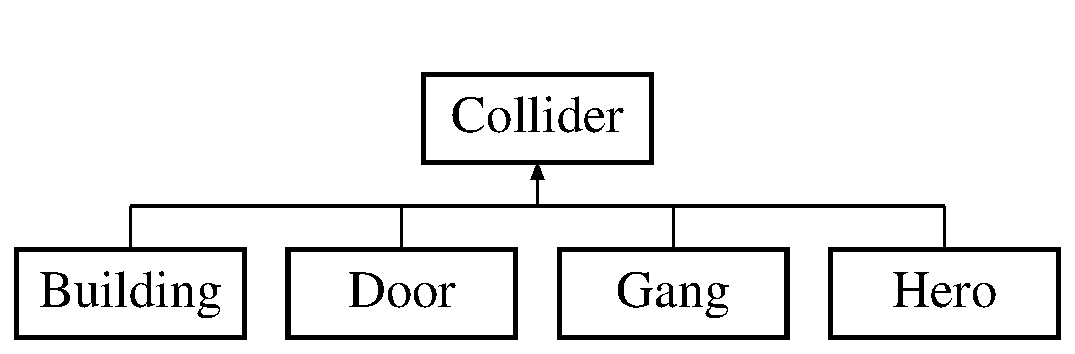
\includegraphics[height=2.000000cm]{class_collider}
\end{center}
\end{figure}
\subsection*{\-Public 멤버 함수}
\begin{DoxyCompactItemize}
\item 
virtual bool \hyperlink{class_collider_aa14301229ec52e3219b41c17ef162925}{check\-\_\-collide} (\hyperlink{class_collider}{\-Collider} $\ast$)=0
\item 
virtual \-S\-D\-L\-\_\-\-Rect $\ast$ \hyperlink{class_collider_a1b6c8bc800070a1e880979378b348e8d}{get\-\_\-box} ()=0
\end{DoxyCompactItemize}


\subsection{멤버 함수 문서화}
\hypertarget{class_collider_aa14301229ec52e3219b41c17ef162925}{\index{\-Collider@{\-Collider}!check\-\_\-collide@{check\-\_\-collide}}
\index{check\-\_\-collide@{check\-\_\-collide}!Collider@{\-Collider}}
\subsubsection[{check\-\_\-collide}]{\setlength{\rightskip}{0pt plus 5cm}virtual bool {\bf \-Collider\-::check\-\_\-collide} (
\begin{DoxyParamCaption}
\item[{{\bf \-Collider} $\ast$}]{}
\end{DoxyParamCaption}
)\hspace{0.3cm}{\ttfamily  \mbox{[}pure virtual\mbox{]}}}}\label{class_collider_aa14301229ec52e3219b41c17ef162925}


\hyperlink{class_gang_ae97a9f4995e999fde4265663e3a838f7}{\-Gang}, \hyperlink{class_hero_a51de873f46281790cc30814fffe0c62c}{\-Hero}, \hyperlink{class_building_a02c1ac48410c20319a30e6ce13433212}{\-Building}, \hyperlink{class_door_a38deff918ee0218bc61a732834591795}{\-Door}에서 구현되었습니다.

\hypertarget{class_collider_a1b6c8bc800070a1e880979378b348e8d}{\index{\-Collider@{\-Collider}!get\-\_\-box@{get\-\_\-box}}
\index{get\-\_\-box@{get\-\_\-box}!Collider@{\-Collider}}
\subsubsection[{get\-\_\-box}]{\setlength{\rightskip}{0pt plus 5cm}virtual \-S\-D\-L\-\_\-\-Rect$\ast$ {\bf \-Collider\-::get\-\_\-box} (
\begin{DoxyParamCaption}
{}
\end{DoxyParamCaption}
)\hspace{0.3cm}{\ttfamily  \mbox{[}pure virtual\mbox{]}}}}\label{class_collider_a1b6c8bc800070a1e880979378b348e8d}


\hyperlink{class_gang_aebd4bd585e284c70b97782ac9af904ee}{\-Gang}, \hyperlink{class_hero_abc32789cc9f1c1374a1d737da8f1a85c}{\-Hero}, \hyperlink{class_building_abb1a4ea20e451db134810c45d530e19f}{\-Building}, \hyperlink{class_door_a2664d8a7636d1eb1e297c8ffd237c379}{\-Door}에서 구현되었습니다.



이 클래스에 대한 문서화 페이지는 다음의 파일로부터 생성되었습니다.\-:\begin{DoxyCompactItemize}
\item 
\hyperlink{collider_8h}{collider.\-h}\end{DoxyCompactItemize}

\hypertarget{class_c_player}{\section{\-C\-Player 클래스 참조}
\label{class_c_player}\index{\-C\-Player@{\-C\-Player}}
}


{\ttfamily \#include $<$\-C\-Player.\-h$>$}

\subsection*{\-Public 타입}
\begin{DoxyCompactItemize}
\item 
typedef std\-::map$<$ int, \hyperlink{class_c_card}{\-C\-Card} $>$ \hyperlink{class_c_player_afc2e175de7122626d649da43d3db40a2}{\-T\-Card\-Inven}
\item 
typedef \-T\-Card\-Inven\-::iterator \hyperlink{class_c_player_a956d26e71ea17e57ac43279eab7eaf3b}{\-T\-Card\-Inven\-Itr}
\end{DoxyCompactItemize}
\subsection*{\-Public 멤버 함수}
\begin{DoxyCompactItemize}
\item 
\hyperlink{class_c_player_a931a59adf2ada5376122e30b33ae2c4c}{\-C\-Player} ()
\item 
void \hyperlink{class_c_player_acf628f08c81409913cb0833bb115cdb3}{\-Reset} (void)
\item 
void \hyperlink{class_c_player_a9913e32cb613756cc092eee3a5b51a2b}{\-Set\-Name} (char $\ast$p\-Name)
\item 
void \hyperlink{class_c_player_a51451db1a48869676883ad6f3f405d14}{\-Set\-Rank} (\hyperlink{_constants_8h_a4db5fb2e90acc4ef6c281d6cca4dea4e}{\-E\-Rank} p\-Rank)
\item 
void \hyperlink{class_c_player_ad57bf753f80586ec0f64c60e0c4ea0fb}{\-Set\-Grade} (unsigned short p\-Grade)
\item 
void \hyperlink{class_c_player_a57cbfab5dbea898e0f1e6d6ef59a299e}{\-Increase\-Grade} (void)
\item 
void \hyperlink{class_c_player_a0fc3b3c7cd8023dbbbdc2b882f0bb332}{\-Decrease\-Grade} (void)
\item 
void \hyperlink{class_c_player_a794b0017abea4805822cd7b45ad87a9b}{\-Add\-Creditor\-Count} (int p\-Count)
\item 
bool \hyperlink{class_c_player_a4649279fe3c5b1f48693f82d96d4f78d}{\-Buy\-Something} (uint64\-\_\-t p\-Price)
\item 
void \hyperlink{class_c_player_a8c6227c3a234b86be05de01cefb5523d}{\-Add\-Dept} (uint64\-\_\-t p\-Dept)
\item 
bool \hyperlink{class_c_player_a18b2124b5135497c522d83b42a003d9f}{\-Add\-Card} (\hyperlink{_constants_8h_a03f7ec9e12b891db1bbeda07eb4099d7}{\-E\-Card} p\-Card)
\item 
bool \hyperlink{class_c_player_ab5eb413c887a4054e7f596f0d579cd9f}{\-Select\-Card} (\hyperlink{_constants_8h_a03f7ec9e12b891db1bbeda07eb4099d7}{\-E\-Card} p\-Card)
\item 
uint64\-\_\-t \hyperlink{class_c_player_a5ab4c5d7ec31884412907a1bbdadad5c}{\-Calc\-Dept} (void)
\item 
const char $\ast$ \hyperlink{class_c_player_a5ae1229e6474d6cf7979d60bdcfbf889}{\-Get\-Player\-Name} (void) const 
\item 
uint64\-\_\-t \hyperlink{class_c_player_a5de57603460102d5ca5c0993d5e7355c}{\-Get\-Dept} (void) const 
\item 
int \hyperlink{class_c_player_a73cd6d410fba5f19c498e58a3df02a90}{\-Get\-Creditor\-Count} (void) const 
\item 
\hyperlink{class_c_player_afc2e175de7122626d649da43d3db40a2}{\-T\-Card\-Inven} $\ast$ \hyperlink{class_c_player_adab4b115cbcac118da7ce6b362de9e0f}{\-Get\-Card\-Inven} (void)
\item 
\hyperlink{class_c_card}{\-C\-Card} $\ast$ \hyperlink{class_c_player_a78464f332f77bee53c7acd94b78c40bb}{\-Get\-Current\-Card} (void)
\item 
\hyperlink{_constants_8h_a4db5fb2e90acc4ef6c281d6cca4dea4e}{\-E\-Rank} \hyperlink{class_c_player_a3837ca31414dc04f376efcf82413293f}{\-Get\-Rank} (void) const 
\item 
unsigned short \hyperlink{class_c_player_aaa70c733b82d5b1145d206282b49e4dc}{\-Get\-Grade} (void) const 
\end{DoxyCompactItemize}


\subsection{멤버 타입정의 문서화}
\hypertarget{class_c_player_afc2e175de7122626d649da43d3db40a2}{\index{\-C\-Player@{\-C\-Player}!\-T\-Card\-Inven@{\-T\-Card\-Inven}}
\index{\-T\-Card\-Inven@{\-T\-Card\-Inven}!CPlayer@{\-C\-Player}}
\subsubsection[{\-T\-Card\-Inven}]{\setlength{\rightskip}{0pt plus 5cm}typedef std\-::map$<$int, {\bf \-C\-Card}$>$ {\bf \-C\-Player\-::\-T\-Card\-Inven}}}\label{class_c_player_afc2e175de7122626d649da43d3db40a2}
\hypertarget{class_c_player_a956d26e71ea17e57ac43279eab7eaf3b}{\index{\-C\-Player@{\-C\-Player}!\-T\-Card\-Inven\-Itr@{\-T\-Card\-Inven\-Itr}}
\index{\-T\-Card\-Inven\-Itr@{\-T\-Card\-Inven\-Itr}!CPlayer@{\-C\-Player}}
\subsubsection[{\-T\-Card\-Inven\-Itr}]{\setlength{\rightskip}{0pt plus 5cm}typedef \-T\-Card\-Inven\-::iterator {\bf \-C\-Player\-::\-T\-Card\-Inven\-Itr}}}\label{class_c_player_a956d26e71ea17e57ac43279eab7eaf3b}


\subsection{생성자 \& 소멸자 문서화}
\hypertarget{class_c_player_a931a59adf2ada5376122e30b33ae2c4c}{\index{\-C\-Player@{\-C\-Player}!\-C\-Player@{\-C\-Player}}
\index{\-C\-Player@{\-C\-Player}!CPlayer@{\-C\-Player}}
\subsubsection[{\-C\-Player}]{\setlength{\rightskip}{0pt plus 5cm}{\bf \-C\-Player\-::\-C\-Player} (
\begin{DoxyParamCaption}
{}
\end{DoxyParamCaption}
)}}\label{class_c_player_a931a59adf2ada5376122e30b33ae2c4c}


\subsection{멤버 함수 문서화}
\hypertarget{class_c_player_a18b2124b5135497c522d83b42a003d9f}{\index{\-C\-Player@{\-C\-Player}!\-Add\-Card@{\-Add\-Card}}
\index{\-Add\-Card@{\-Add\-Card}!CPlayer@{\-C\-Player}}
\subsubsection[{\-Add\-Card}]{\setlength{\rightskip}{0pt plus 5cm}bool {\bf \-C\-Player\-::\-Add\-Card} (
\begin{DoxyParamCaption}
\item[{{\bf \-E\-Card}}]{p\-Card}
\end{DoxyParamCaption}
)}}\label{class_c_player_a18b2124b5135497c522d83b42a003d9f}
\hypertarget{class_c_player_a794b0017abea4805822cd7b45ad87a9b}{\index{\-C\-Player@{\-C\-Player}!\-Add\-Creditor\-Count@{\-Add\-Creditor\-Count}}
\index{\-Add\-Creditor\-Count@{\-Add\-Creditor\-Count}!CPlayer@{\-C\-Player}}
\subsubsection[{\-Add\-Creditor\-Count}]{\setlength{\rightskip}{0pt plus 5cm}void {\bf \-C\-Player\-::\-Add\-Creditor\-Count} (
\begin{DoxyParamCaption}
\item[{int}]{p\-Count}
\end{DoxyParamCaption}
)}}\label{class_c_player_a794b0017abea4805822cd7b45ad87a9b}
\hypertarget{class_c_player_a8c6227c3a234b86be05de01cefb5523d}{\index{\-C\-Player@{\-C\-Player}!\-Add\-Dept@{\-Add\-Dept}}
\index{\-Add\-Dept@{\-Add\-Dept}!CPlayer@{\-C\-Player}}
\subsubsection[{\-Add\-Dept}]{\setlength{\rightskip}{0pt plus 5cm}void {\bf \-C\-Player\-::\-Add\-Dept} (
\begin{DoxyParamCaption}
\item[{uint64\-\_\-t}]{p\-Dept}
\end{DoxyParamCaption}
)}}\label{class_c_player_a8c6227c3a234b86be05de01cefb5523d}
\hypertarget{class_c_player_a4649279fe3c5b1f48693f82d96d4f78d}{\index{\-C\-Player@{\-C\-Player}!\-Buy\-Something@{\-Buy\-Something}}
\index{\-Buy\-Something@{\-Buy\-Something}!CPlayer@{\-C\-Player}}
\subsubsection[{\-Buy\-Something}]{\setlength{\rightskip}{0pt plus 5cm}bool {\bf \-C\-Player\-::\-Buy\-Something} (
\begin{DoxyParamCaption}
\item[{uint64\-\_\-t}]{p\-Price}
\end{DoxyParamCaption}
)}}\label{class_c_player_a4649279fe3c5b1f48693f82d96d4f78d}
\hypertarget{class_c_player_a5ab4c5d7ec31884412907a1bbdadad5c}{\index{\-C\-Player@{\-C\-Player}!\-Calc\-Dept@{\-Calc\-Dept}}
\index{\-Calc\-Dept@{\-Calc\-Dept}!CPlayer@{\-C\-Player}}
\subsubsection[{\-Calc\-Dept}]{\setlength{\rightskip}{0pt plus 5cm}uint64\-\_\-t {\bf \-C\-Player\-::\-Calc\-Dept} (
\begin{DoxyParamCaption}
\item[{void}]{}
\end{DoxyParamCaption}
)}}\label{class_c_player_a5ab4c5d7ec31884412907a1bbdadad5c}
\hypertarget{class_c_player_a0fc3b3c7cd8023dbbbdc2b882f0bb332}{\index{\-C\-Player@{\-C\-Player}!\-Decrease\-Grade@{\-Decrease\-Grade}}
\index{\-Decrease\-Grade@{\-Decrease\-Grade}!CPlayer@{\-C\-Player}}
\subsubsection[{\-Decrease\-Grade}]{\setlength{\rightskip}{0pt plus 5cm}void {\bf \-C\-Player\-::\-Decrease\-Grade} (
\begin{DoxyParamCaption}
\item[{void}]{}
\end{DoxyParamCaption}
)}}\label{class_c_player_a0fc3b3c7cd8023dbbbdc2b882f0bb332}
\hypertarget{class_c_player_adab4b115cbcac118da7ce6b362de9e0f}{\index{\-C\-Player@{\-C\-Player}!\-Get\-Card\-Inven@{\-Get\-Card\-Inven}}
\index{\-Get\-Card\-Inven@{\-Get\-Card\-Inven}!CPlayer@{\-C\-Player}}
\subsubsection[{\-Get\-Card\-Inven}]{\setlength{\rightskip}{0pt plus 5cm}{\bf \-C\-Player\-::\-T\-Card\-Inven} $\ast$ {\bf \-C\-Player\-::\-Get\-Card\-Inven} (
\begin{DoxyParamCaption}
\item[{void}]{}
\end{DoxyParamCaption}
)}}\label{class_c_player_adab4b115cbcac118da7ce6b362de9e0f}
\hypertarget{class_c_player_a73cd6d410fba5f19c498e58a3df02a90}{\index{\-C\-Player@{\-C\-Player}!\-Get\-Creditor\-Count@{\-Get\-Creditor\-Count}}
\index{\-Get\-Creditor\-Count@{\-Get\-Creditor\-Count}!CPlayer@{\-C\-Player}}
\subsubsection[{\-Get\-Creditor\-Count}]{\setlength{\rightskip}{0pt plus 5cm}int {\bf \-C\-Player\-::\-Get\-Creditor\-Count} (
\begin{DoxyParamCaption}
\item[{void}]{}
\end{DoxyParamCaption}
) const}}\label{class_c_player_a73cd6d410fba5f19c498e58a3df02a90}
\hypertarget{class_c_player_a78464f332f77bee53c7acd94b78c40bb}{\index{\-C\-Player@{\-C\-Player}!\-Get\-Current\-Card@{\-Get\-Current\-Card}}
\index{\-Get\-Current\-Card@{\-Get\-Current\-Card}!CPlayer@{\-C\-Player}}
\subsubsection[{\-Get\-Current\-Card}]{\setlength{\rightskip}{0pt plus 5cm}{\bf \-C\-Card} $\ast$ {\bf \-C\-Player\-::\-Get\-Current\-Card} (
\begin{DoxyParamCaption}
\item[{void}]{}
\end{DoxyParamCaption}
)}}\label{class_c_player_a78464f332f77bee53c7acd94b78c40bb}
\hypertarget{class_c_player_a5de57603460102d5ca5c0993d5e7355c}{\index{\-C\-Player@{\-C\-Player}!\-Get\-Dept@{\-Get\-Dept}}
\index{\-Get\-Dept@{\-Get\-Dept}!CPlayer@{\-C\-Player}}
\subsubsection[{\-Get\-Dept}]{\setlength{\rightskip}{0pt plus 5cm}uint64\-\_\-t {\bf \-C\-Player\-::\-Get\-Dept} (
\begin{DoxyParamCaption}
\item[{void}]{}
\end{DoxyParamCaption}
) const}}\label{class_c_player_a5de57603460102d5ca5c0993d5e7355c}
\hypertarget{class_c_player_aaa70c733b82d5b1145d206282b49e4dc}{\index{\-C\-Player@{\-C\-Player}!\-Get\-Grade@{\-Get\-Grade}}
\index{\-Get\-Grade@{\-Get\-Grade}!CPlayer@{\-C\-Player}}
\subsubsection[{\-Get\-Grade}]{\setlength{\rightskip}{0pt plus 5cm}unsigned short {\bf \-C\-Player\-::\-Get\-Grade} (
\begin{DoxyParamCaption}
\item[{void}]{}
\end{DoxyParamCaption}
) const}}\label{class_c_player_aaa70c733b82d5b1145d206282b49e4dc}
\hypertarget{class_c_player_a5ae1229e6474d6cf7979d60bdcfbf889}{\index{\-C\-Player@{\-C\-Player}!\-Get\-Player\-Name@{\-Get\-Player\-Name}}
\index{\-Get\-Player\-Name@{\-Get\-Player\-Name}!CPlayer@{\-C\-Player}}
\subsubsection[{\-Get\-Player\-Name}]{\setlength{\rightskip}{0pt plus 5cm}const char $\ast$ {\bf \-C\-Player\-::\-Get\-Player\-Name} (
\begin{DoxyParamCaption}
\item[{void}]{}
\end{DoxyParamCaption}
) const}}\label{class_c_player_a5ae1229e6474d6cf7979d60bdcfbf889}
\hypertarget{class_c_player_a3837ca31414dc04f376efcf82413293f}{\index{\-C\-Player@{\-C\-Player}!\-Get\-Rank@{\-Get\-Rank}}
\index{\-Get\-Rank@{\-Get\-Rank}!CPlayer@{\-C\-Player}}
\subsubsection[{\-Get\-Rank}]{\setlength{\rightskip}{0pt plus 5cm}{\bf \-E\-Rank} {\bf \-C\-Player\-::\-Get\-Rank} (
\begin{DoxyParamCaption}
\item[{void}]{}
\end{DoxyParamCaption}
) const}}\label{class_c_player_a3837ca31414dc04f376efcf82413293f}
\hypertarget{class_c_player_a57cbfab5dbea898e0f1e6d6ef59a299e}{\index{\-C\-Player@{\-C\-Player}!\-Increase\-Grade@{\-Increase\-Grade}}
\index{\-Increase\-Grade@{\-Increase\-Grade}!CPlayer@{\-C\-Player}}
\subsubsection[{\-Increase\-Grade}]{\setlength{\rightskip}{0pt plus 5cm}void {\bf \-C\-Player\-::\-Increase\-Grade} (
\begin{DoxyParamCaption}
\item[{void}]{}
\end{DoxyParamCaption}
)}}\label{class_c_player_a57cbfab5dbea898e0f1e6d6ef59a299e}
\hypertarget{class_c_player_acf628f08c81409913cb0833bb115cdb3}{\index{\-C\-Player@{\-C\-Player}!\-Reset@{\-Reset}}
\index{\-Reset@{\-Reset}!CPlayer@{\-C\-Player}}
\subsubsection[{\-Reset}]{\setlength{\rightskip}{0pt plus 5cm}void {\bf \-C\-Player\-::\-Reset} (
\begin{DoxyParamCaption}
\item[{void}]{}
\end{DoxyParamCaption}
)}}\label{class_c_player_acf628f08c81409913cb0833bb115cdb3}
\hypertarget{class_c_player_ab5eb413c887a4054e7f596f0d579cd9f}{\index{\-C\-Player@{\-C\-Player}!\-Select\-Card@{\-Select\-Card}}
\index{\-Select\-Card@{\-Select\-Card}!CPlayer@{\-C\-Player}}
\subsubsection[{\-Select\-Card}]{\setlength{\rightskip}{0pt plus 5cm}bool {\bf \-C\-Player\-::\-Select\-Card} (
\begin{DoxyParamCaption}
\item[{{\bf \-E\-Card}}]{p\-Card}
\end{DoxyParamCaption}
)}}\label{class_c_player_ab5eb413c887a4054e7f596f0d579cd9f}
\hypertarget{class_c_player_ad57bf753f80586ec0f64c60e0c4ea0fb}{\index{\-C\-Player@{\-C\-Player}!\-Set\-Grade@{\-Set\-Grade}}
\index{\-Set\-Grade@{\-Set\-Grade}!CPlayer@{\-C\-Player}}
\subsubsection[{\-Set\-Grade}]{\setlength{\rightskip}{0pt plus 5cm}void {\bf \-C\-Player\-::\-Set\-Grade} (
\begin{DoxyParamCaption}
\item[{unsigned short}]{p\-Grade}
\end{DoxyParamCaption}
)}}\label{class_c_player_ad57bf753f80586ec0f64c60e0c4ea0fb}
\hypertarget{class_c_player_a9913e32cb613756cc092eee3a5b51a2b}{\index{\-C\-Player@{\-C\-Player}!\-Set\-Name@{\-Set\-Name}}
\index{\-Set\-Name@{\-Set\-Name}!CPlayer@{\-C\-Player}}
\subsubsection[{\-Set\-Name}]{\setlength{\rightskip}{0pt plus 5cm}void {\bf \-C\-Player\-::\-Set\-Name} (
\begin{DoxyParamCaption}
\item[{char $\ast$}]{p\-Name}
\end{DoxyParamCaption}
)}}\label{class_c_player_a9913e32cb613756cc092eee3a5b51a2b}
\hypertarget{class_c_player_a51451db1a48869676883ad6f3f405d14}{\index{\-C\-Player@{\-C\-Player}!\-Set\-Rank@{\-Set\-Rank}}
\index{\-Set\-Rank@{\-Set\-Rank}!CPlayer@{\-C\-Player}}
\subsubsection[{\-Set\-Rank}]{\setlength{\rightskip}{0pt plus 5cm}void {\bf \-C\-Player\-::\-Set\-Rank} (
\begin{DoxyParamCaption}
\item[{{\bf \-E\-Rank}}]{p\-Rank}
\end{DoxyParamCaption}
)}}\label{class_c_player_a51451db1a48869676883ad6f3f405d14}


이 클래스에 대한 문서화 페이지는 다음의 파일들로부터 생성되었습니다.\-:\begin{DoxyCompactItemize}
\item 
\hyperlink{_c_player_8h}{\-C\-Player.\-h}\item 
\hyperlink{_c_player_8cpp}{\-C\-Player.\-cpp}\end{DoxyCompactItemize}

\hypertarget{class_credit_scene}{\section{\-Credit\-Scene 클래스 참조}
\label{class_credit_scene}\index{\-Credit\-Scene@{\-Credit\-Scene}}
}


{\ttfamily \#include $<$\-Scene.\-h$>$}

\-Credit\-Scene에 대한 상속 다이어그램 \-: \begin{figure}[H]
\begin{center}
\leavevmode
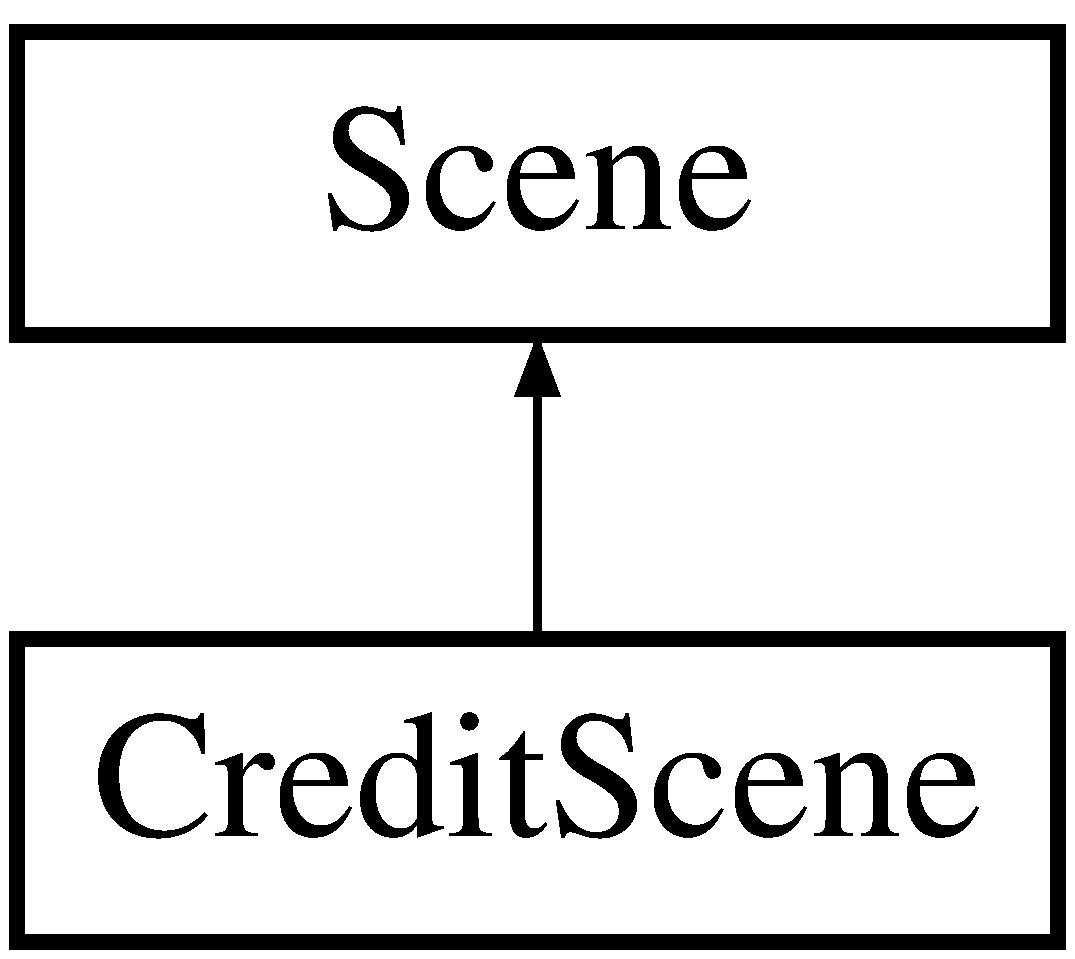
\includegraphics[height=2.000000cm]{class_credit_scene}
\end{center}
\end{figure}
\subsection*{\-Public 멤버 함수}
\begin{DoxyCompactItemize}
\item 
\hyperlink{class_credit_scene_a4b191906d6fe649b3acb94422e17645c}{\-Credit\-Scene} ()
\item 
virtual void \hyperlink{class_credit_scene_a565f227f48dbdb61858b85f362a23d6a}{init} ()
\item 
virtual void \hyperlink{class_credit_scene_a51294d71978f451fba4cf1c2e9617d51}{clean\-\_\-up} ()
\item 
virtual void \hyperlink{class_credit_scene_af465a04b7ec8b7f6cc157d8f86740af6}{do\-\_\-event} ()
\item 
virtual void \hyperlink{class_credit_scene_a9a6f9d39dbdb43510295522679b20b1e}{show} ()
\end{DoxyCompactItemize}


\subsection{생성자 \& 소멸자 문서화}
\hypertarget{class_credit_scene_a4b191906d6fe649b3acb94422e17645c}{\index{\-Credit\-Scene@{\-Credit\-Scene}!\-Credit\-Scene@{\-Credit\-Scene}}
\index{\-Credit\-Scene@{\-Credit\-Scene}!CreditScene@{\-Credit\-Scene}}
\subsubsection[{\-Credit\-Scene}]{\setlength{\rightskip}{0pt plus 5cm}{\bf \-Credit\-Scene\-::\-Credit\-Scene} (
\begin{DoxyParamCaption}
{}
\end{DoxyParamCaption}
)}}\label{class_credit_scene_a4b191906d6fe649b3acb94422e17645c}


\subsection{멤버 함수 문서화}
\hypertarget{class_credit_scene_a51294d71978f451fba4cf1c2e9617d51}{\index{\-Credit\-Scene@{\-Credit\-Scene}!clean\-\_\-up@{clean\-\_\-up}}
\index{clean\-\_\-up@{clean\-\_\-up}!CreditScene@{\-Credit\-Scene}}
\subsubsection[{clean\-\_\-up}]{\setlength{\rightskip}{0pt plus 5cm}void {\bf \-Credit\-Scene\-::clean\-\_\-up} (
\begin{DoxyParamCaption}
{}
\end{DoxyParamCaption}
)\hspace{0.3cm}{\ttfamily  \mbox{[}virtual\mbox{]}}}}\label{class_credit_scene_a51294d71978f451fba4cf1c2e9617d51}


\hyperlink{class_scene_a5f8c03499f5adff28224ccaaf95a8d90}{\-Scene}(으)로부터 재구현되었습니다.

\hypertarget{class_credit_scene_af465a04b7ec8b7f6cc157d8f86740af6}{\index{\-Credit\-Scene@{\-Credit\-Scene}!do\-\_\-event@{do\-\_\-event}}
\index{do\-\_\-event@{do\-\_\-event}!CreditScene@{\-Credit\-Scene}}
\subsubsection[{do\-\_\-event}]{\setlength{\rightskip}{0pt plus 5cm}void {\bf \-Credit\-Scene\-::do\-\_\-event} (
\begin{DoxyParamCaption}
{}
\end{DoxyParamCaption}
)\hspace{0.3cm}{\ttfamily  \mbox{[}virtual\mbox{]}}}}\label{class_credit_scene_af465a04b7ec8b7f6cc157d8f86740af6}


\hyperlink{class_scene_a280970a0176e70f76d2420c50261d6fa}{\-Scene}(으)로부터 재구현되었습니다.

\hypertarget{class_credit_scene_a565f227f48dbdb61858b85f362a23d6a}{\index{\-Credit\-Scene@{\-Credit\-Scene}!init@{init}}
\index{init@{init}!CreditScene@{\-Credit\-Scene}}
\subsubsection[{init}]{\setlength{\rightskip}{0pt plus 5cm}void {\bf \-Credit\-Scene\-::init} (
\begin{DoxyParamCaption}
{}
\end{DoxyParamCaption}
)\hspace{0.3cm}{\ttfamily  \mbox{[}virtual\mbox{]}}}}\label{class_credit_scene_a565f227f48dbdb61858b85f362a23d6a}


\hyperlink{class_scene_abb3b6efc6fdba03cd96436edaf08a967}{\-Scene}(으)로부터 재구현되었습니다.

\hypertarget{class_credit_scene_a9a6f9d39dbdb43510295522679b20b1e}{\index{\-Credit\-Scene@{\-Credit\-Scene}!show@{show}}
\index{show@{show}!CreditScene@{\-Credit\-Scene}}
\subsubsection[{show}]{\setlength{\rightskip}{0pt plus 5cm}void {\bf \-Credit\-Scene\-::show} (
\begin{DoxyParamCaption}
{}
\end{DoxyParamCaption}
)\hspace{0.3cm}{\ttfamily  \mbox{[}virtual\mbox{]}}}}\label{class_credit_scene_a9a6f9d39dbdb43510295522679b20b1e}


\hyperlink{class_scene_a6f447a90b1f9009acfb72df711473875}{\-Scene}(으)로부터 재구현되었습니다.



이 클래스에 대한 문서화 페이지는 다음의 파일들로부터 생성되었습니다.\-:\begin{DoxyCompactItemize}
\item 
\hyperlink{_scene_8h}{\-Scene.\-h}\item 
\hyperlink{_scene_8cpp}{\-Scene.\-cpp}\end{DoxyCompactItemize}

\hypertarget{class_door}{\section{\-Door 클래스 참조}
\label{class_door}\index{\-Door@{\-Door}}
}


{\ttfamily \#include $<$building.\-h$>$}

\-Door에 대한 상속 다이어그램 \-: \begin{figure}[H]
\begin{center}
\leavevmode
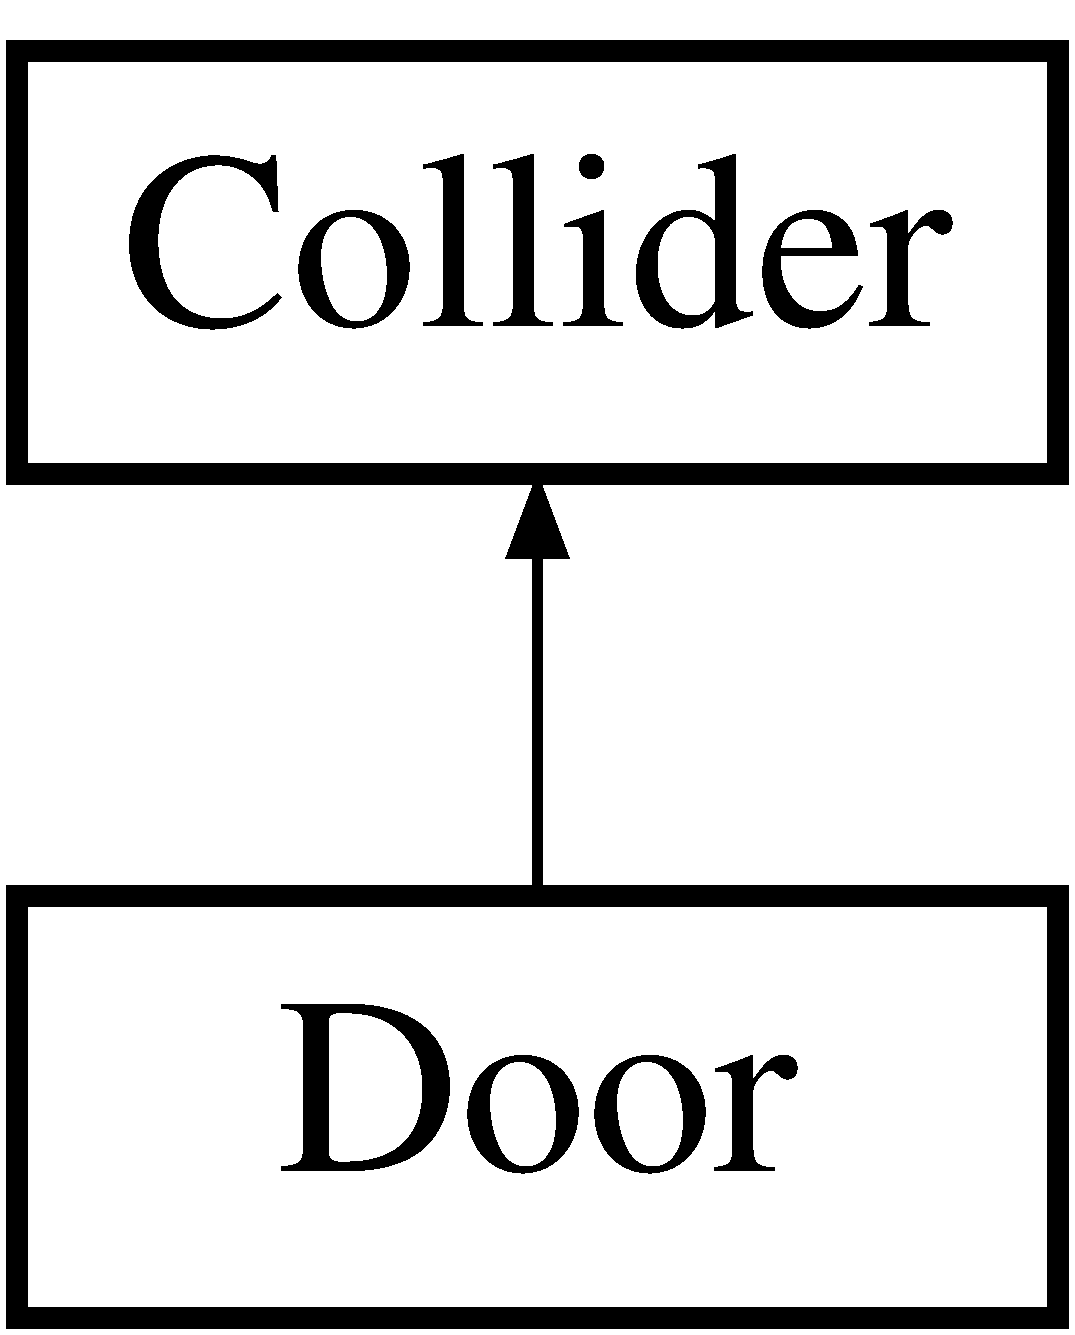
\includegraphics[height=2.000000cm]{class_door}
\end{center}
\end{figure}
\subsection*{\-Public 멤버 함수}
\begin{DoxyCompactItemize}
\item 
\hyperlink{class_door_a494e2d4a8fdd198e2229b066e5473997}{\-Door} (int building\-\_\-x, int building\-\_\-y, int \-\_\-x=\hyperlink{global_8h_aca0bd9ade5788664bbf47fc95c52f9bb}{\-D\-O\-O\-R\-\_\-\-X}, int \-\_\-y=\hyperlink{global_8h_a2070dd4270c9575cdcd0f507d75104d0}{\-D\-O\-O\-R\-\_\-\-Y}, int \-\_\-w=\hyperlink{global_8h_ac41cbf633f73b0077c07daf186768497}{\-D\-O\-O\-R\-\_\-\-W}, int \-\_\-h=\hyperlink{global_8h_a1989de9fa88a8b55e0c7b7a77f6913f9}{\-D\-O\-O\-R\-\_\-\-H})
\item 
virtual bool \hyperlink{class_door_a38deff918ee0218bc61a732834591795}{check\-\_\-collide} (\hyperlink{class_collider}{\-Collider} $\ast$)
\item 
virtual \-S\-D\-L\-\_\-\-Rect $\ast$ \hyperlink{class_door_a2664d8a7636d1eb1e297c8ffd237c379}{get\-\_\-box} ()
\end{DoxyCompactItemize}


\subsection{생성자 \& 소멸자 문서화}
\hypertarget{class_door_a494e2d4a8fdd198e2229b066e5473997}{\index{\-Door@{\-Door}!\-Door@{\-Door}}
\index{\-Door@{\-Door}!Door@{\-Door}}
\subsubsection[{\-Door}]{\setlength{\rightskip}{0pt plus 5cm}{\bf \-Door\-::\-Door} (
\begin{DoxyParamCaption}
\item[{int}]{building\-\_\-x, }
\item[{int}]{building\-\_\-y, }
\item[{int}]{\-\_\-x = {\ttfamily {\bf \-D\-O\-O\-R\-\_\-\-X}}, }
\item[{int}]{\-\_\-y = {\ttfamily {\bf \-D\-O\-O\-R\-\_\-\-Y}}, }
\item[{int}]{\-\_\-w = {\ttfamily {\bf \-D\-O\-O\-R\-\_\-\-W}}, }
\item[{int}]{\-\_\-h = {\ttfamily {\bf \-D\-O\-O\-R\-\_\-\-H}}}
\end{DoxyParamCaption}
)}}\label{class_door_a494e2d4a8fdd198e2229b066e5473997}


\subsection{멤버 함수 문서화}
\hypertarget{class_door_a38deff918ee0218bc61a732834591795}{\index{\-Door@{\-Door}!check\-\_\-collide@{check\-\_\-collide}}
\index{check\-\_\-collide@{check\-\_\-collide}!Door@{\-Door}}
\subsubsection[{check\-\_\-collide}]{\setlength{\rightskip}{0pt plus 5cm}bool {\bf \-Door\-::check\-\_\-collide} (
\begin{DoxyParamCaption}
\item[{{\bf \-Collider} $\ast$}]{other}
\end{DoxyParamCaption}
)\hspace{0.3cm}{\ttfamily  \mbox{[}virtual\mbox{]}}}}\label{class_door_a38deff918ee0218bc61a732834591795}


\hyperlink{class_collider_aa14301229ec52e3219b41c17ef162925}{\-Collider}를 구현.

\hypertarget{class_door_a2664d8a7636d1eb1e297c8ffd237c379}{\index{\-Door@{\-Door}!get\-\_\-box@{get\-\_\-box}}
\index{get\-\_\-box@{get\-\_\-box}!Door@{\-Door}}
\subsubsection[{get\-\_\-box}]{\setlength{\rightskip}{0pt plus 5cm}\-S\-D\-L\-\_\-\-Rect $\ast$ {\bf \-Door\-::get\-\_\-box} (
\begin{DoxyParamCaption}
{}
\end{DoxyParamCaption}
)\hspace{0.3cm}{\ttfamily  \mbox{[}virtual\mbox{]}}}}\label{class_door_a2664d8a7636d1eb1e297c8ffd237c379}


\hyperlink{class_collider_a1b6c8bc800070a1e880979378b348e8d}{\-Collider}를 구현.



이 클래스에 대한 문서화 페이지는 다음의 파일들로부터 생성되었습니다.\-:\begin{DoxyCompactItemize}
\item 
\hyperlink{building_8h}{building.\-h}\item 
\hyperlink{building_8cpp}{building.\-cpp}\end{DoxyCompactItemize}

\hypertarget{class_game_scene}{\section{\-Game\-Scene 클래스 참조}
\label{class_game_scene}\index{\-Game\-Scene@{\-Game\-Scene}}
}


{\ttfamily \#include $<$\-Scene.\-h$>$}

\-Game\-Scene에 대한 상속 다이어그램 \-: \begin{figure}[H]
\begin{center}
\leavevmode
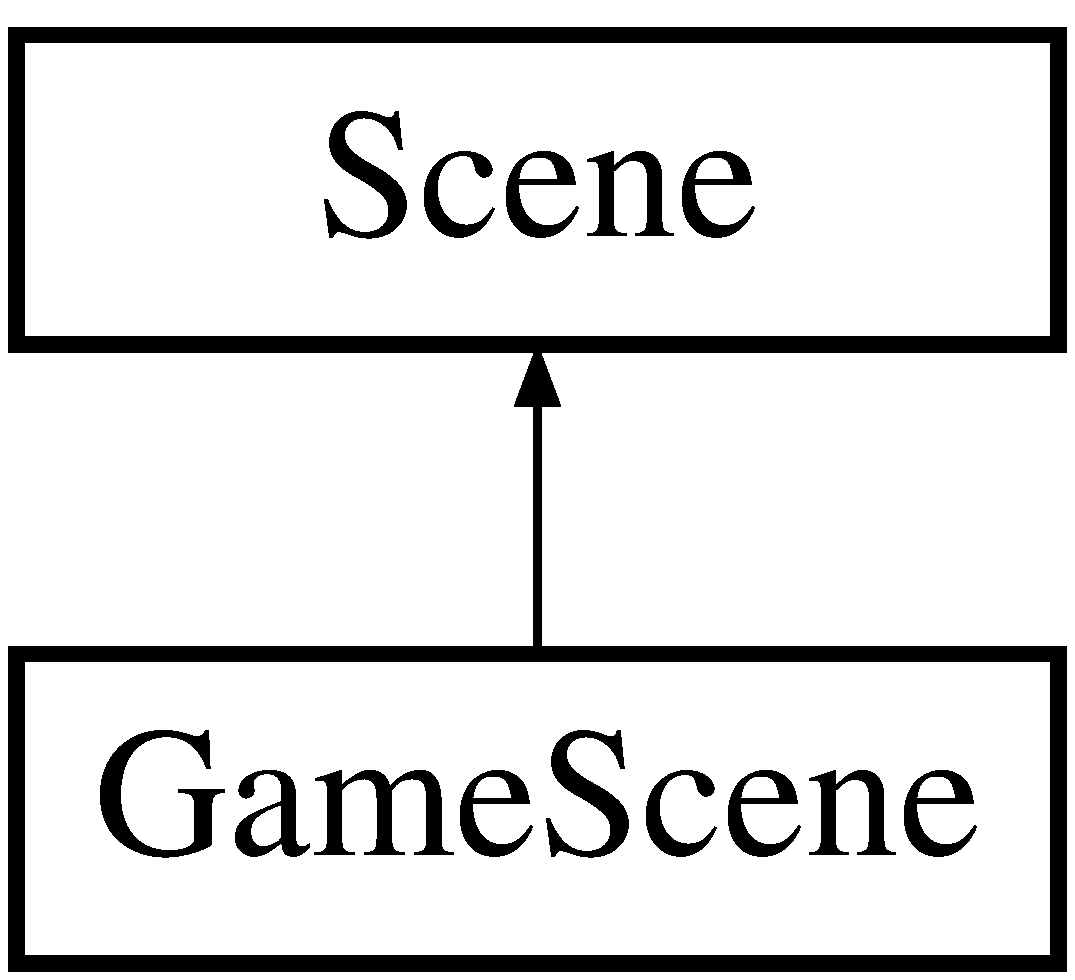
\includegraphics[height=2.000000cm]{class_game_scene}
\end{center}
\end{figure}
\subsection*{\-Public 멤버 함수}
\begin{DoxyCompactItemize}
\item 
\hyperlink{class_game_scene_ac53cc300c8896048c0e21c67e49681b9}{\-Game\-Scene} ()
\item 
virtual void \hyperlink{class_game_scene_ae379e50ebfc2b3cc53906e9d8a11b1d2}{init} ()
\item 
virtual void \hyperlink{class_game_scene_a1e341f7ef5fc4659ee00828ce5be753b}{clean\-\_\-up} ()
\item 
virtual void \hyperlink{class_game_scene_add4701b7cc4649c5eee8f98ac273286a}{do\-\_\-event} ()
\item 
virtual void \hyperlink{class_game_scene_a17ab02461114e20f681d73a9b2528532}{show} ()
\item 
void \hyperlink{class_game_scene_ae5757dc11e6053d29b276489da88ad3b}{show\-\_\-message\-\_\-box} ()
\item 
void \hyperlink{class_game_scene_a0500a8d3803534b399d9095b81b827e3}{check\-\_\-collide} ()
\item 
void \hyperlink{class_game_scene_aca6b89a4a0d33b2c230a379c1c65966b}{print\-\_\-message\-\_\-1} (std\-::string msg)
\item 
void \hyperlink{class_game_scene_ab61c9c7abe60d2b6cdcecdea0aea3444}{print\-\_\-message\-\_\-2} (std\-::string msg)
\end{DoxyCompactItemize}


\subsection{생성자 \& 소멸자 문서화}
\hypertarget{class_game_scene_ac53cc300c8896048c0e21c67e49681b9}{\index{\-Game\-Scene@{\-Game\-Scene}!\-Game\-Scene@{\-Game\-Scene}}
\index{\-Game\-Scene@{\-Game\-Scene}!GameScene@{\-Game\-Scene}}
\subsubsection[{\-Game\-Scene}]{\setlength{\rightskip}{0pt plus 5cm}{\bf \-Game\-Scene\-::\-Game\-Scene} (
\begin{DoxyParamCaption}
{}
\end{DoxyParamCaption}
)}}\label{class_game_scene_ac53cc300c8896048c0e21c67e49681b9}


\subsection{멤버 함수 문서화}
\hypertarget{class_game_scene_a0500a8d3803534b399d9095b81b827e3}{\index{\-Game\-Scene@{\-Game\-Scene}!check\-\_\-collide@{check\-\_\-collide}}
\index{check\-\_\-collide@{check\-\_\-collide}!GameScene@{\-Game\-Scene}}
\subsubsection[{check\-\_\-collide}]{\setlength{\rightskip}{0pt plus 5cm}void {\bf \-Game\-Scene\-::check\-\_\-collide} (
\begin{DoxyParamCaption}
{}
\end{DoxyParamCaption}
)}}\label{class_game_scene_a0500a8d3803534b399d9095b81b827e3}
\hypertarget{class_game_scene_a1e341f7ef5fc4659ee00828ce5be753b}{\index{\-Game\-Scene@{\-Game\-Scene}!clean\-\_\-up@{clean\-\_\-up}}
\index{clean\-\_\-up@{clean\-\_\-up}!GameScene@{\-Game\-Scene}}
\subsubsection[{clean\-\_\-up}]{\setlength{\rightskip}{0pt plus 5cm}void {\bf \-Game\-Scene\-::clean\-\_\-up} (
\begin{DoxyParamCaption}
{}
\end{DoxyParamCaption}
)\hspace{0.3cm}{\ttfamily  \mbox{[}virtual\mbox{]}}}}\label{class_game_scene_a1e341f7ef5fc4659ee00828ce5be753b}


\hyperlink{class_scene_a5f8c03499f5adff28224ccaaf95a8d90}{\-Scene}(으)로부터 재구현되었습니다.

\hypertarget{class_game_scene_add4701b7cc4649c5eee8f98ac273286a}{\index{\-Game\-Scene@{\-Game\-Scene}!do\-\_\-event@{do\-\_\-event}}
\index{do\-\_\-event@{do\-\_\-event}!GameScene@{\-Game\-Scene}}
\subsubsection[{do\-\_\-event}]{\setlength{\rightskip}{0pt plus 5cm}void {\bf \-Game\-Scene\-::do\-\_\-event} (
\begin{DoxyParamCaption}
{}
\end{DoxyParamCaption}
)\hspace{0.3cm}{\ttfamily  \mbox{[}virtual\mbox{]}}}}\label{class_game_scene_add4701b7cc4649c5eee8f98ac273286a}


\hyperlink{class_scene_a280970a0176e70f76d2420c50261d6fa}{\-Scene}(으)로부터 재구현되었습니다.

\hypertarget{class_game_scene_ae379e50ebfc2b3cc53906e9d8a11b1d2}{\index{\-Game\-Scene@{\-Game\-Scene}!init@{init}}
\index{init@{init}!GameScene@{\-Game\-Scene}}
\subsubsection[{init}]{\setlength{\rightskip}{0pt plus 5cm}void {\bf \-Game\-Scene\-::init} (
\begin{DoxyParamCaption}
{}
\end{DoxyParamCaption}
)\hspace{0.3cm}{\ttfamily  \mbox{[}virtual\mbox{]}}}}\label{class_game_scene_ae379e50ebfc2b3cc53906e9d8a11b1d2}


\hyperlink{class_scene_abb3b6efc6fdba03cd96436edaf08a967}{\-Scene}(으)로부터 재구현되었습니다.

\hypertarget{class_game_scene_aca6b89a4a0d33b2c230a379c1c65966b}{\index{\-Game\-Scene@{\-Game\-Scene}!print\-\_\-message\-\_\-1@{print\-\_\-message\-\_\-1}}
\index{print\-\_\-message\-\_\-1@{print\-\_\-message\-\_\-1}!GameScene@{\-Game\-Scene}}
\subsubsection[{print\-\_\-message\-\_\-1}]{\setlength{\rightskip}{0pt plus 5cm}void {\bf \-Game\-Scene\-::print\-\_\-message\-\_\-1} (
\begin{DoxyParamCaption}
\item[{std\-::string}]{msg}
\end{DoxyParamCaption}
)}}\label{class_game_scene_aca6b89a4a0d33b2c230a379c1c65966b}
\hypertarget{class_game_scene_ab61c9c7abe60d2b6cdcecdea0aea3444}{\index{\-Game\-Scene@{\-Game\-Scene}!print\-\_\-message\-\_\-2@{print\-\_\-message\-\_\-2}}
\index{print\-\_\-message\-\_\-2@{print\-\_\-message\-\_\-2}!GameScene@{\-Game\-Scene}}
\subsubsection[{print\-\_\-message\-\_\-2}]{\setlength{\rightskip}{0pt plus 5cm}void {\bf \-Game\-Scene\-::print\-\_\-message\-\_\-2} (
\begin{DoxyParamCaption}
\item[{std\-::string}]{msg}
\end{DoxyParamCaption}
)}}\label{class_game_scene_ab61c9c7abe60d2b6cdcecdea0aea3444}
\hypertarget{class_game_scene_a17ab02461114e20f681d73a9b2528532}{\index{\-Game\-Scene@{\-Game\-Scene}!show@{show}}
\index{show@{show}!GameScene@{\-Game\-Scene}}
\subsubsection[{show}]{\setlength{\rightskip}{0pt plus 5cm}void {\bf \-Game\-Scene\-::show} (
\begin{DoxyParamCaption}
{}
\end{DoxyParamCaption}
)\hspace{0.3cm}{\ttfamily  \mbox{[}virtual\mbox{]}}}}\label{class_game_scene_a17ab02461114e20f681d73a9b2528532}


\hyperlink{class_scene_a6f447a90b1f9009acfb72df711473875}{\-Scene}(으)로부터 재구현되었습니다.

\hypertarget{class_game_scene_ae5757dc11e6053d29b276489da88ad3b}{\index{\-Game\-Scene@{\-Game\-Scene}!show\-\_\-message\-\_\-box@{show\-\_\-message\-\_\-box}}
\index{show\-\_\-message\-\_\-box@{show\-\_\-message\-\_\-box}!GameScene@{\-Game\-Scene}}
\subsubsection[{show\-\_\-message\-\_\-box}]{\setlength{\rightskip}{0pt plus 5cm}void {\bf \-Game\-Scene\-::show\-\_\-message\-\_\-box} (
\begin{DoxyParamCaption}
{}
\end{DoxyParamCaption}
)}}\label{class_game_scene_ae5757dc11e6053d29b276489da88ad3b}


이 클래스에 대한 문서화 페이지는 다음의 파일들로부터 생성되었습니다.\-:\begin{DoxyCompactItemize}
\item 
\hyperlink{_scene_8h}{\-Scene.\-h}\item 
\hyperlink{_game_scene_8cpp}{\-Game\-Scene.\-cpp}\end{DoxyCompactItemize}

\hypertarget{class_gang}{\section{\-Gang 클래스 참조}
\label{class_gang}\index{\-Gang@{\-Gang}}
}


{\ttfamily \#include $<$character.\-h$>$}

\-Gang에 대한 상속 다이어그램 \-: \begin{figure}[H]
\begin{center}
\leavevmode
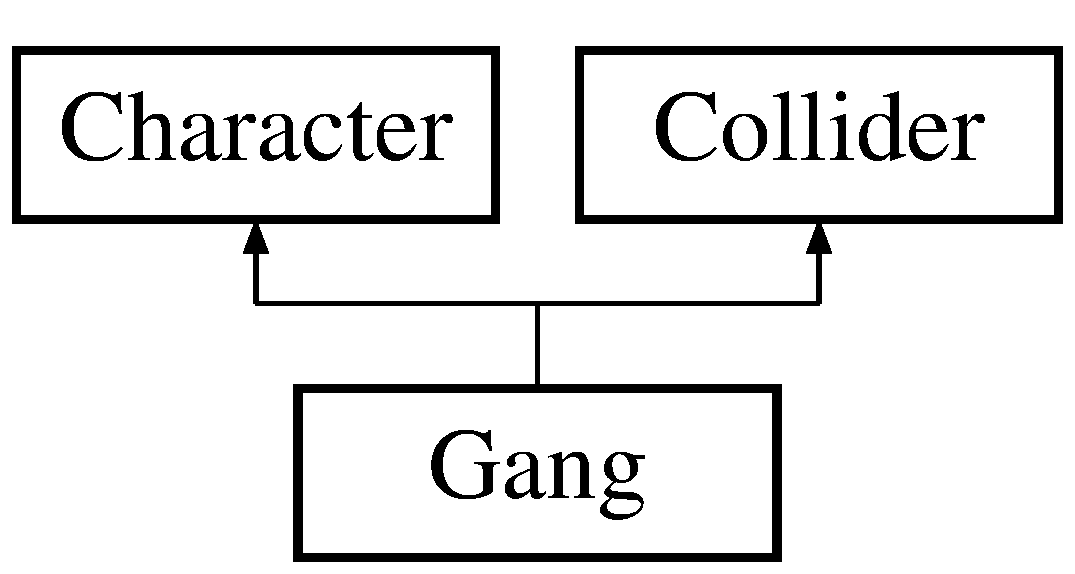
\includegraphics[height=2.000000cm]{class_gang}
\end{center}
\end{figure}
\subsection*{\-Public 멤버 함수}
\begin{DoxyCompactItemize}
\item 
virtual void \hyperlink{class_gang_a3788b8ace6c57cdcdc464a2f96169484}{init} ()
\item 
virtual void \hyperlink{class_gang_af472124b9a8c3e4a5950562342ec8162}{clean\-\_\-up} ()
\item 
virtual bool \hyperlink{class_gang_abccb863ee9ef936fad5031a0d93e1b55}{move} (\-Uint32 delta\-Ticks)
\item 
virtual void \hyperlink{class_gang_a29330bf2df1bd60644513b2cb27f29e6}{show} (\-S\-D\-L\-\_\-\-Surface $\ast$)
\item 
virtual void \hyperlink{class_gang_af4463fb95507a172b1495fae411bfba5}{set\-\_\-clip} ()
\item 
virtual void \hyperlink{class_gang_ad177257ab75d22c409b6b7b89c5d0870}{add\-\_\-person} ()
\item 
virtual bool \hyperlink{class_gang_ae97a9f4995e999fde4265663e3a838f7}{check\-\_\-collide} (\hyperlink{class_collider}{\-Collider} $\ast$)
\item 
virtual \-S\-D\-L\-\_\-\-Rect $\ast$ \hyperlink{class_gang_aebd4bd585e284c70b97782ac9af904ee}{get\-\_\-box} ()
\item 
virtual void \hyperlink{class_gang_a74c369149d11573fbad437d997266c36}{set\-\_\-object} (\-S\-D\-L\-\_\-\-Rect $\ast$object)
\item 
virtual void \hyperlink{class_gang_ac3aa2c0e70ecf1e7ce42192f684d1398}{move\-\_\-back} ()
\item 
bool \hyperlink{class_gang_a9984bed5cfe0541a97e00e2972666bae}{follow} ()
\end{DoxyCompactItemize}


\subsection{멤버 함수 문서화}
\hypertarget{class_gang_ad177257ab75d22c409b6b7b89c5d0870}{\index{\-Gang@{\-Gang}!add\-\_\-person@{add\-\_\-person}}
\index{add\-\_\-person@{add\-\_\-person}!Gang@{\-Gang}}
\subsubsection[{add\-\_\-person}]{\setlength{\rightskip}{0pt plus 5cm}void {\bf \-Gang\-::add\-\_\-person} (
\begin{DoxyParamCaption}
{}
\end{DoxyParamCaption}
)\hspace{0.3cm}{\ttfamily  \mbox{[}virtual\mbox{]}}}}\label{class_gang_ad177257ab75d22c409b6b7b89c5d0870}


\hyperlink{class_character_a074348cfffee21b386e6ed3d950a7f2f}{\-Character}(으)로부터 재구현되었습니다.

\hypertarget{class_gang_ae97a9f4995e999fde4265663e3a838f7}{\index{\-Gang@{\-Gang}!check\-\_\-collide@{check\-\_\-collide}}
\index{check\-\_\-collide@{check\-\_\-collide}!Gang@{\-Gang}}
\subsubsection[{check\-\_\-collide}]{\setlength{\rightskip}{0pt plus 5cm}bool {\bf \-Gang\-::check\-\_\-collide} (
\begin{DoxyParamCaption}
\item[{{\bf \-Collider} $\ast$}]{other}
\end{DoxyParamCaption}
)\hspace{0.3cm}{\ttfamily  \mbox{[}virtual\mbox{]}}}}\label{class_gang_ae97a9f4995e999fde4265663e3a838f7}


\hyperlink{class_collider_aa14301229ec52e3219b41c17ef162925}{\-Collider}를 구현.

\hypertarget{class_gang_af472124b9a8c3e4a5950562342ec8162}{\index{\-Gang@{\-Gang}!clean\-\_\-up@{clean\-\_\-up}}
\index{clean\-\_\-up@{clean\-\_\-up}!Gang@{\-Gang}}
\subsubsection[{clean\-\_\-up}]{\setlength{\rightskip}{0pt plus 5cm}void {\bf \-Gang\-::clean\-\_\-up} (
\begin{DoxyParamCaption}
{}
\end{DoxyParamCaption}
)\hspace{0.3cm}{\ttfamily  \mbox{[}virtual\mbox{]}}}}\label{class_gang_af472124b9a8c3e4a5950562342ec8162}


\hyperlink{class_character_a2304027ce7b4caf5a1851e371f3071cd}{\-Character}(으)로부터 재구현되었습니다.

\hypertarget{class_gang_a9984bed5cfe0541a97e00e2972666bae}{\index{\-Gang@{\-Gang}!follow@{follow}}
\index{follow@{follow}!Gang@{\-Gang}}
\subsubsection[{follow}]{\setlength{\rightskip}{0pt plus 5cm}bool {\bf \-Gang\-::follow} (
\begin{DoxyParamCaption}
{}
\end{DoxyParamCaption}
)}}\label{class_gang_a9984bed5cfe0541a97e00e2972666bae}
\hypertarget{class_gang_aebd4bd585e284c70b97782ac9af904ee}{\index{\-Gang@{\-Gang}!get\-\_\-box@{get\-\_\-box}}
\index{get\-\_\-box@{get\-\_\-box}!Gang@{\-Gang}}
\subsubsection[{get\-\_\-box}]{\setlength{\rightskip}{0pt plus 5cm}\-S\-D\-L\-\_\-\-Rect $\ast$ {\bf \-Gang\-::get\-\_\-box} (
\begin{DoxyParamCaption}
{}
\end{DoxyParamCaption}
)\hspace{0.3cm}{\ttfamily  \mbox{[}virtual\mbox{]}}}}\label{class_gang_aebd4bd585e284c70b97782ac9af904ee}


\hyperlink{class_collider_a1b6c8bc800070a1e880979378b348e8d}{\-Collider}를 구현.

\hypertarget{class_gang_a3788b8ace6c57cdcdc464a2f96169484}{\index{\-Gang@{\-Gang}!init@{init}}
\index{init@{init}!Gang@{\-Gang}}
\subsubsection[{init}]{\setlength{\rightskip}{0pt plus 5cm}void {\bf \-Gang\-::init} (
\begin{DoxyParamCaption}
{}
\end{DoxyParamCaption}
)\hspace{0.3cm}{\ttfamily  \mbox{[}virtual\mbox{]}}}}\label{class_gang_a3788b8ace6c57cdcdc464a2f96169484}


\hyperlink{class_character_ae026a3baf7b9a31c270b9b0596c5e181}{\-Character}(으)로부터 재구현되었습니다.

\hypertarget{class_gang_abccb863ee9ef936fad5031a0d93e1b55}{\index{\-Gang@{\-Gang}!move@{move}}
\index{move@{move}!Gang@{\-Gang}}
\subsubsection[{move}]{\setlength{\rightskip}{0pt plus 5cm}bool {\bf \-Gang\-::move} (
\begin{DoxyParamCaption}
\item[{\-Uint32}]{delta\-Ticks}
\end{DoxyParamCaption}
)\hspace{0.3cm}{\ttfamily  \mbox{[}virtual\mbox{]}}}}\label{class_gang_abccb863ee9ef936fad5031a0d93e1b55}


\hyperlink{class_character_a32f64bd79aac4bcdfa3878b34ffd39da}{\-Character}(으)로부터 재구현되었습니다.

\hypertarget{class_gang_ac3aa2c0e70ecf1e7ce42192f684d1398}{\index{\-Gang@{\-Gang}!move\-\_\-back@{move\-\_\-back}}
\index{move\-\_\-back@{move\-\_\-back}!Gang@{\-Gang}}
\subsubsection[{move\-\_\-back}]{\setlength{\rightskip}{0pt plus 5cm}void {\bf \-Gang\-::move\-\_\-back} (
\begin{DoxyParamCaption}
{}
\end{DoxyParamCaption}
)\hspace{0.3cm}{\ttfamily  \mbox{[}virtual\mbox{]}}}}\label{class_gang_ac3aa2c0e70ecf1e7ce42192f684d1398}


\hyperlink{class_character_a33e738893b424f6e890f49d756c7ffe6}{\-Character}(으)로부터 재구현되었습니다.

\hypertarget{class_gang_af4463fb95507a172b1495fae411bfba5}{\index{\-Gang@{\-Gang}!set\-\_\-clip@{set\-\_\-clip}}
\index{set\-\_\-clip@{set\-\_\-clip}!Gang@{\-Gang}}
\subsubsection[{set\-\_\-clip}]{\setlength{\rightskip}{0pt plus 5cm}void {\bf \-Gang\-::set\-\_\-clip} (
\begin{DoxyParamCaption}
{}
\end{DoxyParamCaption}
)\hspace{0.3cm}{\ttfamily  \mbox{[}virtual\mbox{]}}}}\label{class_gang_af4463fb95507a172b1495fae411bfba5}


\hyperlink{class_character_ae29d39664b615ddee1fd855569cade90}{\-Character}(으)로부터 재구현되었습니다.

\hypertarget{class_gang_a74c369149d11573fbad437d997266c36}{\index{\-Gang@{\-Gang}!set\-\_\-object@{set\-\_\-object}}
\index{set\-\_\-object@{set\-\_\-object}!Gang@{\-Gang}}
\subsubsection[{set\-\_\-object}]{\setlength{\rightskip}{0pt plus 5cm}void {\bf \-Gang\-::set\-\_\-object} (
\begin{DoxyParamCaption}
\item[{\-S\-D\-L\-\_\-\-Rect $\ast$}]{object}
\end{DoxyParamCaption}
)\hspace{0.3cm}{\ttfamily  \mbox{[}virtual\mbox{]}}}}\label{class_gang_a74c369149d11573fbad437d997266c36}


\hyperlink{class_character_a24e66bb11b377efa0079393d6ed99e89}{\-Character}(으)로부터 재구현되었습니다.

\hypertarget{class_gang_a29330bf2df1bd60644513b2cb27f29e6}{\index{\-Gang@{\-Gang}!show@{show}}
\index{show@{show}!Gang@{\-Gang}}
\subsubsection[{show}]{\setlength{\rightskip}{0pt plus 5cm}void {\bf \-Gang\-::show} (
\begin{DoxyParamCaption}
\item[{\-S\-D\-L\-\_\-\-Surface $\ast$}]{screen}
\end{DoxyParamCaption}
)\hspace{0.3cm}{\ttfamily  \mbox{[}virtual\mbox{]}}}}\label{class_gang_a29330bf2df1bd60644513b2cb27f29e6}


\hyperlink{class_character_aee8d4cab5de7363e08ebcaf14171a454}{\-Character}(으)로부터 재구현되었습니다.



이 클래스에 대한 문서화 페이지는 다음의 파일들로부터 생성되었습니다.\-:\begin{DoxyCompactItemize}
\item 
\hyperlink{character_8h}{character.\-h}\item 
\hyperlink{gang_8cpp}{gang.\-cpp}\end{DoxyCompactItemize}

\hypertarget{class_good_end_scene}{\section{\-Good\-End\-Scene 클래스 참조}
\label{class_good_end_scene}\index{\-Good\-End\-Scene@{\-Good\-End\-Scene}}
}


{\ttfamily \#include $<$\-Scene.\-h$>$}

\-Good\-End\-Scene에 대한 상속 다이어그램 \-: \begin{figure}[H]
\begin{center}
\leavevmode
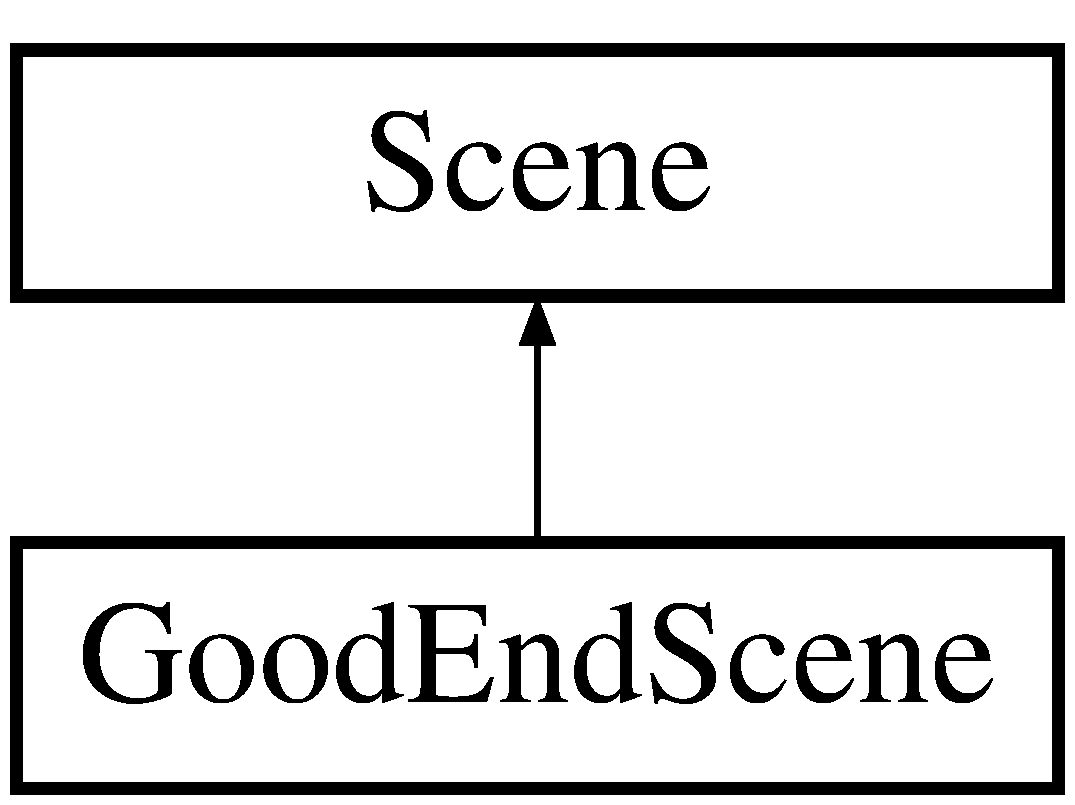
\includegraphics[height=2.000000cm]{class_good_end_scene}
\end{center}
\end{figure}
\subsection*{\-Public 멤버 함수}
\begin{DoxyCompactItemize}
\item 
\hyperlink{class_good_end_scene_ad04c0002e9c7cff656c6ece640ccc55e}{\-Good\-End\-Scene} ()
\item 
virtual void \hyperlink{class_good_end_scene_a63feec1f4ee968e29cf04a6c499360c3}{init} ()
\item 
virtual void \hyperlink{class_good_end_scene_ab3d4faec409c826ee0f6a2752ac60dee}{clean\-\_\-up} ()
\item 
virtual void \hyperlink{class_good_end_scene_a2015e80af48f0e7aa53dc1186dc173e9}{do\-\_\-event} ()
\item 
virtual void \hyperlink{class_good_end_scene_a29207c910451e85aab64796959ad8e6d}{show} ()
\end{DoxyCompactItemize}


\subsection{생성자 \& 소멸자 문서화}
\hypertarget{class_good_end_scene_ad04c0002e9c7cff656c6ece640ccc55e}{\index{\-Good\-End\-Scene@{\-Good\-End\-Scene}!\-Good\-End\-Scene@{\-Good\-End\-Scene}}
\index{\-Good\-End\-Scene@{\-Good\-End\-Scene}!GoodEndScene@{\-Good\-End\-Scene}}
\subsubsection[{\-Good\-End\-Scene}]{\setlength{\rightskip}{0pt plus 5cm}{\bf \-Good\-End\-Scene\-::\-Good\-End\-Scene} (
\begin{DoxyParamCaption}
{}
\end{DoxyParamCaption}
)}}\label{class_good_end_scene_ad04c0002e9c7cff656c6ece640ccc55e}


\subsection{멤버 함수 문서화}
\hypertarget{class_good_end_scene_ab3d4faec409c826ee0f6a2752ac60dee}{\index{\-Good\-End\-Scene@{\-Good\-End\-Scene}!clean\-\_\-up@{clean\-\_\-up}}
\index{clean\-\_\-up@{clean\-\_\-up}!GoodEndScene@{\-Good\-End\-Scene}}
\subsubsection[{clean\-\_\-up}]{\setlength{\rightskip}{0pt plus 5cm}void {\bf \-Good\-End\-Scene\-::clean\-\_\-up} (
\begin{DoxyParamCaption}
{}
\end{DoxyParamCaption}
)\hspace{0.3cm}{\ttfamily  \mbox{[}virtual\mbox{]}}}}\label{class_good_end_scene_ab3d4faec409c826ee0f6a2752ac60dee}


\hyperlink{class_scene_a5f8c03499f5adff28224ccaaf95a8d90}{\-Scene}(으)로부터 재구현되었습니다.

\hypertarget{class_good_end_scene_a2015e80af48f0e7aa53dc1186dc173e9}{\index{\-Good\-End\-Scene@{\-Good\-End\-Scene}!do\-\_\-event@{do\-\_\-event}}
\index{do\-\_\-event@{do\-\_\-event}!GoodEndScene@{\-Good\-End\-Scene}}
\subsubsection[{do\-\_\-event}]{\setlength{\rightskip}{0pt plus 5cm}void {\bf \-Good\-End\-Scene\-::do\-\_\-event} (
\begin{DoxyParamCaption}
{}
\end{DoxyParamCaption}
)\hspace{0.3cm}{\ttfamily  \mbox{[}virtual\mbox{]}}}}\label{class_good_end_scene_a2015e80af48f0e7aa53dc1186dc173e9}


\hyperlink{class_scene_a280970a0176e70f76d2420c50261d6fa}{\-Scene}(으)로부터 재구현되었습니다.

\hypertarget{class_good_end_scene_a63feec1f4ee968e29cf04a6c499360c3}{\index{\-Good\-End\-Scene@{\-Good\-End\-Scene}!init@{init}}
\index{init@{init}!GoodEndScene@{\-Good\-End\-Scene}}
\subsubsection[{init}]{\setlength{\rightskip}{0pt plus 5cm}void {\bf \-Good\-End\-Scene\-::init} (
\begin{DoxyParamCaption}
{}
\end{DoxyParamCaption}
)\hspace{0.3cm}{\ttfamily  \mbox{[}virtual\mbox{]}}}}\label{class_good_end_scene_a63feec1f4ee968e29cf04a6c499360c3}


\hyperlink{class_scene_abb3b6efc6fdba03cd96436edaf08a967}{\-Scene}(으)로부터 재구현되었습니다.

\hypertarget{class_good_end_scene_a29207c910451e85aab64796959ad8e6d}{\index{\-Good\-End\-Scene@{\-Good\-End\-Scene}!show@{show}}
\index{show@{show}!GoodEndScene@{\-Good\-End\-Scene}}
\subsubsection[{show}]{\setlength{\rightskip}{0pt plus 5cm}void {\bf \-Good\-End\-Scene\-::show} (
\begin{DoxyParamCaption}
{}
\end{DoxyParamCaption}
)\hspace{0.3cm}{\ttfamily  \mbox{[}virtual\mbox{]}}}}\label{class_good_end_scene_a29207c910451e85aab64796959ad8e6d}


\hyperlink{class_scene_a6f447a90b1f9009acfb72df711473875}{\-Scene}(으)로부터 재구현되었습니다.



이 클래스에 대한 문서화 페이지는 다음의 파일들로부터 생성되었습니다.\-:\begin{DoxyCompactItemize}
\item 
\hyperlink{_scene_8h}{\-Scene.\-h}\item 
\hyperlink{_scene_8cpp}{\-Scene.\-cpp}\end{DoxyCompactItemize}

\hypertarget{class_hero}{\section{\-Hero 클래스 참조}
\label{class_hero}\index{\-Hero@{\-Hero}}
}


{\ttfamily \#include $<$character.\-h$>$}

\-Hero에 대한 상속 다이어그램 \-: \begin{figure}[H]
\begin{center}
\leavevmode
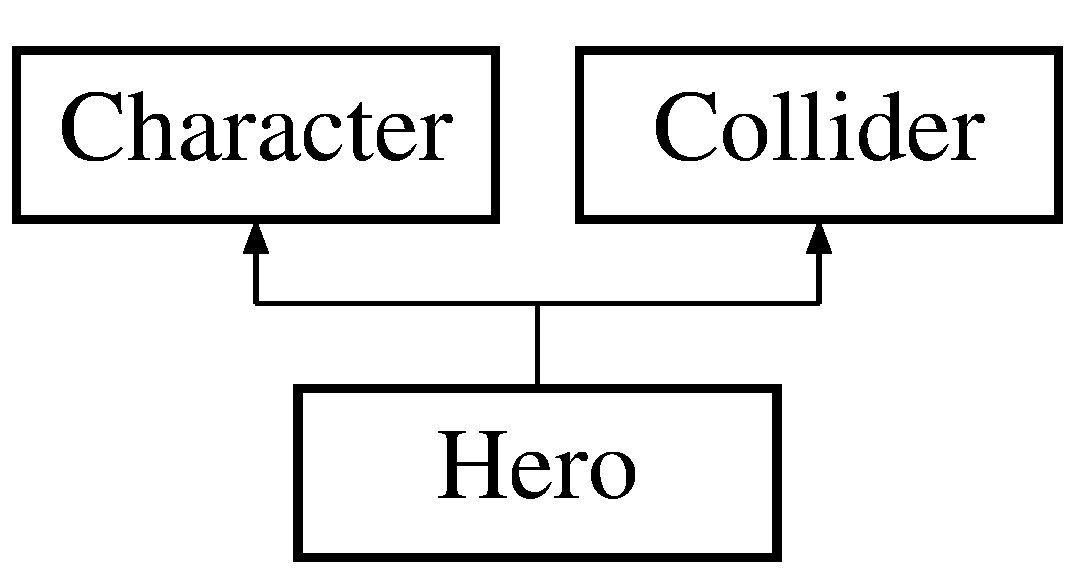
\includegraphics[height=2.000000cm]{class_hero}
\end{center}
\end{figure}
\subsection*{\-Public 멤버 함수}
\begin{DoxyCompactItemize}
\item 
virtual void \hyperlink{class_hero_ae67cc4b7770083755895b78664d0ea34}{init} ()
\item 
virtual void \hyperlink{class_hero_a43836f7e926f00a4a27757a1ff7410a0}{clean\-\_\-up} ()
\item 
virtual bool \hyperlink{class_hero_a0961b6b66165095e3d764ccc60436846}{move} (\-Uint32 delta\-Ticks)
\item 
virtual void \hyperlink{class_hero_a9670c2232f5bf0f66bba60a7c747c53d}{show} (\-S\-D\-L\-\_\-\-Surface $\ast$)
\item 
virtual void \hyperlink{class_hero_aa5bde5d2f4a3d086b9e8ce2b969e2f3f}{set\-\_\-clip} ()
\item 
virtual void \hyperlink{class_hero_aa8934d60bc26f9eefdc15661d924e5e0}{add\-\_\-person} ()
\item 
virtual bool \hyperlink{class_hero_a51de873f46281790cc30814fffe0c62c}{check\-\_\-collide} (\hyperlink{class_collider}{\-Collider} $\ast$)
\item 
virtual \-S\-D\-L\-\_\-\-Rect $\ast$ \hyperlink{class_hero_abc32789cc9f1c1374a1d737da8f1a85c}{get\-\_\-box} ()
\item 
void \hyperlink{class_hero_a61e221d7b3ddfa81363ef1617d288b62}{handle\-Input} ()
\item 
void \hyperlink{class_hero_a9871bf08a8a2a4d739b59ccccf23a164}{can\-\_\-buy} ()
\item 
void \hyperlink{class_hero_a59e335e5c9169ea1055f49c89a2d965b}{cant\-\_\-buy} ()
\item 
bool \hyperlink{class_hero_af42a20265af06855ca1fdca1f82ed3c2}{buy} ()
\item 
virtual void \hyperlink{class_hero_a805934d28498398aecb10f8d2de6b63e}{move\-\_\-back} ()
\item 
uint64\-\_\-t \hyperlink{class_hero_ad12877233a3a18ae6db1ad758375bb2c}{get\-\_\-depth} ()
\item 
int \hyperlink{class_hero_a1c333d4e29923e655229eaf44178b3b9}{calc\-\_\-dept} ()
\item 
void \hyperlink{class_hero_a942b64ba1d1e3e5be2be79d0d737a83e}{add\-\_\-card} (\hyperlink{_constants_8h_a03f7ec9e12b891db1bbeda07eb4099d7}{\-E\-Card} p\-Card)
\item 
void \hyperlink{class_hero_a4b3ac843ddfeaed8d4138d4d6507b13a}{select\-\_\-card} (\hyperlink{_constants_8h_a03f7ec9e12b891db1bbeda07eb4099d7}{\-E\-Card} p\-Card)
\item 
\hyperlink{_constants_8h_a03f7ec9e12b891db1bbeda07eb4099d7}{\-E\-Card} \hyperlink{class_hero_a067b9cf2010d54ea54ce583dcebc0a38}{get\-\_\-current\-\_\-card} ()
\item 
uint64\-\_\-t \hyperlink{class_hero_ab20de0bd528c4de19e7e1a67ee4d4aba}{get\-\_\-limit} ()
\item 
bool \hyperlink{class_hero_abcf5ca4897f949e4e8e2bb83fc99bb53}{has\-\_\-card} ()
\item 
unsigned short \hyperlink{class_hero_a41aa0f6885d0bf1e8b2bf5dd2a51818c}{get\-\_\-grade} ()
\item 
void \hyperlink{class_hero_a4f3e7b14d65aba9f8660406792972713}{decrease\-\_\-grade} ()
\item 
void \hyperlink{class_hero_a18e875ed1fb65a5f0a900b1173658027}{increase\-\_\-grade} ()
\end{DoxyCompactItemize}


\subsection{멤버 함수 문서화}
\hypertarget{class_hero_a942b64ba1d1e3e5be2be79d0d737a83e}{\index{\-Hero@{\-Hero}!add\-\_\-card@{add\-\_\-card}}
\index{add\-\_\-card@{add\-\_\-card}!Hero@{\-Hero}}
\subsubsection[{add\-\_\-card}]{\setlength{\rightskip}{0pt plus 5cm}void {\bf \-Hero\-::add\-\_\-card} (
\begin{DoxyParamCaption}
\item[{{\bf \-E\-Card}}]{p\-Card}
\end{DoxyParamCaption}
)}}\label{class_hero_a942b64ba1d1e3e5be2be79d0d737a83e}
\hypertarget{class_hero_aa8934d60bc26f9eefdc15661d924e5e0}{\index{\-Hero@{\-Hero}!add\-\_\-person@{add\-\_\-person}}
\index{add\-\_\-person@{add\-\_\-person}!Hero@{\-Hero}}
\subsubsection[{add\-\_\-person}]{\setlength{\rightskip}{0pt plus 5cm}void {\bf \-Hero\-::add\-\_\-person} (
\begin{DoxyParamCaption}
{}
\end{DoxyParamCaption}
)\hspace{0.3cm}{\ttfamily  \mbox{[}virtual\mbox{]}}}}\label{class_hero_aa8934d60bc26f9eefdc15661d924e5e0}


\hyperlink{class_character_a074348cfffee21b386e6ed3d950a7f2f}{\-Character}(으)로부터 재구현되었습니다.

\hypertarget{class_hero_af42a20265af06855ca1fdca1f82ed3c2}{\index{\-Hero@{\-Hero}!buy@{buy}}
\index{buy@{buy}!Hero@{\-Hero}}
\subsubsection[{buy}]{\setlength{\rightskip}{0pt plus 5cm}bool {\bf \-Hero\-::buy} (
\begin{DoxyParamCaption}
{}
\end{DoxyParamCaption}
)}}\label{class_hero_af42a20265af06855ca1fdca1f82ed3c2}
\hypertarget{class_hero_a1c333d4e29923e655229eaf44178b3b9}{\index{\-Hero@{\-Hero}!calc\-\_\-dept@{calc\-\_\-dept}}
\index{calc\-\_\-dept@{calc\-\_\-dept}!Hero@{\-Hero}}
\subsubsection[{calc\-\_\-dept}]{\setlength{\rightskip}{0pt plus 5cm}int {\bf \-Hero\-::calc\-\_\-dept} (
\begin{DoxyParamCaption}
{}
\end{DoxyParamCaption}
)}}\label{class_hero_a1c333d4e29923e655229eaf44178b3b9}
\hypertarget{class_hero_a9871bf08a8a2a4d739b59ccccf23a164}{\index{\-Hero@{\-Hero}!can\-\_\-buy@{can\-\_\-buy}}
\index{can\-\_\-buy@{can\-\_\-buy}!Hero@{\-Hero}}
\subsubsection[{can\-\_\-buy}]{\setlength{\rightskip}{0pt plus 5cm}void {\bf \-Hero\-::can\-\_\-buy} (
\begin{DoxyParamCaption}
{}
\end{DoxyParamCaption}
)}}\label{class_hero_a9871bf08a8a2a4d739b59ccccf23a164}
\hypertarget{class_hero_a59e335e5c9169ea1055f49c89a2d965b}{\index{\-Hero@{\-Hero}!cant\-\_\-buy@{cant\-\_\-buy}}
\index{cant\-\_\-buy@{cant\-\_\-buy}!Hero@{\-Hero}}
\subsubsection[{cant\-\_\-buy}]{\setlength{\rightskip}{0pt plus 5cm}void {\bf \-Hero\-::cant\-\_\-buy} (
\begin{DoxyParamCaption}
{}
\end{DoxyParamCaption}
)}}\label{class_hero_a59e335e5c9169ea1055f49c89a2d965b}
\hypertarget{class_hero_a51de873f46281790cc30814fffe0c62c}{\index{\-Hero@{\-Hero}!check\-\_\-collide@{check\-\_\-collide}}
\index{check\-\_\-collide@{check\-\_\-collide}!Hero@{\-Hero}}
\subsubsection[{check\-\_\-collide}]{\setlength{\rightskip}{0pt plus 5cm}bool {\bf \-Hero\-::check\-\_\-collide} (
\begin{DoxyParamCaption}
\item[{{\bf \-Collider} $\ast$}]{other}
\end{DoxyParamCaption}
)\hspace{0.3cm}{\ttfamily  \mbox{[}virtual\mbox{]}}}}\label{class_hero_a51de873f46281790cc30814fffe0c62c}


\hyperlink{class_collider_aa14301229ec52e3219b41c17ef162925}{\-Collider}를 구현.

\hypertarget{class_hero_a43836f7e926f00a4a27757a1ff7410a0}{\index{\-Hero@{\-Hero}!clean\-\_\-up@{clean\-\_\-up}}
\index{clean\-\_\-up@{clean\-\_\-up}!Hero@{\-Hero}}
\subsubsection[{clean\-\_\-up}]{\setlength{\rightskip}{0pt plus 5cm}void {\bf \-Hero\-::clean\-\_\-up} (
\begin{DoxyParamCaption}
{}
\end{DoxyParamCaption}
)\hspace{0.3cm}{\ttfamily  \mbox{[}virtual\mbox{]}}}}\label{class_hero_a43836f7e926f00a4a27757a1ff7410a0}


\hyperlink{class_character_a2304027ce7b4caf5a1851e371f3071cd}{\-Character}(으)로부터 재구현되었습니다.

\hypertarget{class_hero_a4f3e7b14d65aba9f8660406792972713}{\index{\-Hero@{\-Hero}!decrease\-\_\-grade@{decrease\-\_\-grade}}
\index{decrease\-\_\-grade@{decrease\-\_\-grade}!Hero@{\-Hero}}
\subsubsection[{decrease\-\_\-grade}]{\setlength{\rightskip}{0pt plus 5cm}void {\bf \-Hero\-::decrease\-\_\-grade} (
\begin{DoxyParamCaption}
{}
\end{DoxyParamCaption}
)}}\label{class_hero_a4f3e7b14d65aba9f8660406792972713}
\hypertarget{class_hero_abc32789cc9f1c1374a1d737da8f1a85c}{\index{\-Hero@{\-Hero}!get\-\_\-box@{get\-\_\-box}}
\index{get\-\_\-box@{get\-\_\-box}!Hero@{\-Hero}}
\subsubsection[{get\-\_\-box}]{\setlength{\rightskip}{0pt plus 5cm}\-S\-D\-L\-\_\-\-Rect $\ast$ {\bf \-Hero\-::get\-\_\-box} (
\begin{DoxyParamCaption}
{}
\end{DoxyParamCaption}
)\hspace{0.3cm}{\ttfamily  \mbox{[}virtual\mbox{]}}}}\label{class_hero_abc32789cc9f1c1374a1d737da8f1a85c}


\hyperlink{class_collider_a1b6c8bc800070a1e880979378b348e8d}{\-Collider}를 구현.

\hypertarget{class_hero_a067b9cf2010d54ea54ce583dcebc0a38}{\index{\-Hero@{\-Hero}!get\-\_\-current\-\_\-card@{get\-\_\-current\-\_\-card}}
\index{get\-\_\-current\-\_\-card@{get\-\_\-current\-\_\-card}!Hero@{\-Hero}}
\subsubsection[{get\-\_\-current\-\_\-card}]{\setlength{\rightskip}{0pt plus 5cm}{\bf \-E\-Card} {\bf \-Hero\-::get\-\_\-current\-\_\-card} (
\begin{DoxyParamCaption}
{}
\end{DoxyParamCaption}
)}}\label{class_hero_a067b9cf2010d54ea54ce583dcebc0a38}
\hypertarget{class_hero_ad12877233a3a18ae6db1ad758375bb2c}{\index{\-Hero@{\-Hero}!get\-\_\-depth@{get\-\_\-depth}}
\index{get\-\_\-depth@{get\-\_\-depth}!Hero@{\-Hero}}
\subsubsection[{get\-\_\-depth}]{\setlength{\rightskip}{0pt plus 5cm}uint64\-\_\-t {\bf \-Hero\-::get\-\_\-depth} (
\begin{DoxyParamCaption}
{}
\end{DoxyParamCaption}
)}}\label{class_hero_ad12877233a3a18ae6db1ad758375bb2c}
\hypertarget{class_hero_a41aa0f6885d0bf1e8b2bf5dd2a51818c}{\index{\-Hero@{\-Hero}!get\-\_\-grade@{get\-\_\-grade}}
\index{get\-\_\-grade@{get\-\_\-grade}!Hero@{\-Hero}}
\subsubsection[{get\-\_\-grade}]{\setlength{\rightskip}{0pt plus 5cm}unsigned short {\bf \-Hero\-::get\-\_\-grade} (
\begin{DoxyParamCaption}
{}
\end{DoxyParamCaption}
)}}\label{class_hero_a41aa0f6885d0bf1e8b2bf5dd2a51818c}
\hypertarget{class_hero_ab20de0bd528c4de19e7e1a67ee4d4aba}{\index{\-Hero@{\-Hero}!get\-\_\-limit@{get\-\_\-limit}}
\index{get\-\_\-limit@{get\-\_\-limit}!Hero@{\-Hero}}
\subsubsection[{get\-\_\-limit}]{\setlength{\rightskip}{0pt plus 5cm}uint64\-\_\-t {\bf \-Hero\-::get\-\_\-limit} (
\begin{DoxyParamCaption}
{}
\end{DoxyParamCaption}
)}}\label{class_hero_ab20de0bd528c4de19e7e1a67ee4d4aba}
\hypertarget{class_hero_a61e221d7b3ddfa81363ef1617d288b62}{\index{\-Hero@{\-Hero}!handle\-Input@{handle\-Input}}
\index{handle\-Input@{handle\-Input}!Hero@{\-Hero}}
\subsubsection[{handle\-Input}]{\setlength{\rightskip}{0pt plus 5cm}void {\bf \-Hero\-::handle\-Input} (
\begin{DoxyParamCaption}
{}
\end{DoxyParamCaption}
)}}\label{class_hero_a61e221d7b3ddfa81363ef1617d288b62}
\hypertarget{class_hero_abcf5ca4897f949e4e8e2bb83fc99bb53}{\index{\-Hero@{\-Hero}!has\-\_\-card@{has\-\_\-card}}
\index{has\-\_\-card@{has\-\_\-card}!Hero@{\-Hero}}
\subsubsection[{has\-\_\-card}]{\setlength{\rightskip}{0pt plus 5cm}bool {\bf \-Hero\-::has\-\_\-card} (
\begin{DoxyParamCaption}
{}
\end{DoxyParamCaption}
)}}\label{class_hero_abcf5ca4897f949e4e8e2bb83fc99bb53}
\hypertarget{class_hero_a18e875ed1fb65a5f0a900b1173658027}{\index{\-Hero@{\-Hero}!increase\-\_\-grade@{increase\-\_\-grade}}
\index{increase\-\_\-grade@{increase\-\_\-grade}!Hero@{\-Hero}}
\subsubsection[{increase\-\_\-grade}]{\setlength{\rightskip}{0pt plus 5cm}void {\bf \-Hero\-::increase\-\_\-grade} (
\begin{DoxyParamCaption}
{}
\end{DoxyParamCaption}
)}}\label{class_hero_a18e875ed1fb65a5f0a900b1173658027}
\hypertarget{class_hero_ae67cc4b7770083755895b78664d0ea34}{\index{\-Hero@{\-Hero}!init@{init}}
\index{init@{init}!Hero@{\-Hero}}
\subsubsection[{init}]{\setlength{\rightskip}{0pt plus 5cm}void {\bf \-Hero\-::init} (
\begin{DoxyParamCaption}
{}
\end{DoxyParamCaption}
)\hspace{0.3cm}{\ttfamily  \mbox{[}virtual\mbox{]}}}}\label{class_hero_ae67cc4b7770083755895b78664d0ea34}


\hyperlink{class_character_ae026a3baf7b9a31c270b9b0596c5e181}{\-Character}(으)로부터 재구현되었습니다.

\hypertarget{class_hero_a0961b6b66165095e3d764ccc60436846}{\index{\-Hero@{\-Hero}!move@{move}}
\index{move@{move}!Hero@{\-Hero}}
\subsubsection[{move}]{\setlength{\rightskip}{0pt plus 5cm}bool {\bf \-Hero\-::move} (
\begin{DoxyParamCaption}
\item[{\-Uint32}]{delta\-Ticks}
\end{DoxyParamCaption}
)\hspace{0.3cm}{\ttfamily  \mbox{[}virtual\mbox{]}}}}\label{class_hero_a0961b6b66165095e3d764ccc60436846}


\hyperlink{class_character_a32f64bd79aac4bcdfa3878b34ffd39da}{\-Character}(으)로부터 재구현되었습니다.

\hypertarget{class_hero_a805934d28498398aecb10f8d2de6b63e}{\index{\-Hero@{\-Hero}!move\-\_\-back@{move\-\_\-back}}
\index{move\-\_\-back@{move\-\_\-back}!Hero@{\-Hero}}
\subsubsection[{move\-\_\-back}]{\setlength{\rightskip}{0pt plus 5cm}void {\bf \-Hero\-::move\-\_\-back} (
\begin{DoxyParamCaption}
{}
\end{DoxyParamCaption}
)\hspace{0.3cm}{\ttfamily  \mbox{[}virtual\mbox{]}}}}\label{class_hero_a805934d28498398aecb10f8d2de6b63e}


\hyperlink{class_character_a33e738893b424f6e890f49d756c7ffe6}{\-Character}(으)로부터 재구현되었습니다.

\hypertarget{class_hero_a4b3ac843ddfeaed8d4138d4d6507b13a}{\index{\-Hero@{\-Hero}!select\-\_\-card@{select\-\_\-card}}
\index{select\-\_\-card@{select\-\_\-card}!Hero@{\-Hero}}
\subsubsection[{select\-\_\-card}]{\setlength{\rightskip}{0pt plus 5cm}void {\bf \-Hero\-::select\-\_\-card} (
\begin{DoxyParamCaption}
\item[{{\bf \-E\-Card}}]{p\-Card}
\end{DoxyParamCaption}
)}}\label{class_hero_a4b3ac843ddfeaed8d4138d4d6507b13a}
\hypertarget{class_hero_aa5bde5d2f4a3d086b9e8ce2b969e2f3f}{\index{\-Hero@{\-Hero}!set\-\_\-clip@{set\-\_\-clip}}
\index{set\-\_\-clip@{set\-\_\-clip}!Hero@{\-Hero}}
\subsubsection[{set\-\_\-clip}]{\setlength{\rightskip}{0pt plus 5cm}void {\bf \-Hero\-::set\-\_\-clip} (
\begin{DoxyParamCaption}
{}
\end{DoxyParamCaption}
)\hspace{0.3cm}{\ttfamily  \mbox{[}virtual\mbox{]}}}}\label{class_hero_aa5bde5d2f4a3d086b9e8ce2b969e2f3f}


\hyperlink{class_character_ae29d39664b615ddee1fd855569cade90}{\-Character}(으)로부터 재구현되었습니다.

\hypertarget{class_hero_a9670c2232f5bf0f66bba60a7c747c53d}{\index{\-Hero@{\-Hero}!show@{show}}
\index{show@{show}!Hero@{\-Hero}}
\subsubsection[{show}]{\setlength{\rightskip}{0pt plus 5cm}void {\bf \-Hero\-::show} (
\begin{DoxyParamCaption}
\item[{\-S\-D\-L\-\_\-\-Surface $\ast$}]{screen}
\end{DoxyParamCaption}
)\hspace{0.3cm}{\ttfamily  \mbox{[}virtual\mbox{]}}}}\label{class_hero_a9670c2232f5bf0f66bba60a7c747c53d}


\hyperlink{class_character_aee8d4cab5de7363e08ebcaf14171a454}{\-Character}(으)로부터 재구현되었습니다.



이 클래스에 대한 문서화 페이지는 다음의 파일들로부터 생성되었습니다.\-:\begin{DoxyCompactItemize}
\item 
\hyperlink{character_8h}{character.\-h}\item 
\hyperlink{character_8cpp}{character.\-cpp}\end{DoxyCompactItemize}

\hypertarget{structlua___debug}{\section{lua\-\_\-\-Debug 구조체 참조}
\label{structlua___debug}\index{lua\-\_\-\-Debug@{lua\-\_\-\-Debug}}
}


{\ttfamily \#include $<$lua.\-h$>$}

\subsection*{\-Public 속성}
\begin{DoxyCompactItemize}
\item 
int \hyperlink{structlua___debug_a6578d385d2322429a0fe87b79f1ddec0}{event}
\item 
const char $\ast$ \hyperlink{structlua___debug_a2978ab7f2ade479a003beb16d3b7a993}{name}
\item 
const char $\ast$ \hyperlink{structlua___debug_a7e8c201950ea4dd3f2c7df9e1201019a}{namewhat}
\item 
const char $\ast$ \hyperlink{structlua___debug_afbf8df5f26e9c345378a7eb402eed081}{what}
\item 
const char $\ast$ \hyperlink{structlua___debug_a422bceba8605d96bce4d19ce801a62e4}{source}
\item 
int \hyperlink{structlua___debug_a97b3ed36cdfdc6f2c694b253a3d96da6}{currentline}
\item 
int \hyperlink{structlua___debug_a983807ecf0dfa3e5e77fe7f0e2fd9d49}{nups}
\item 
int \hyperlink{structlua___debug_a97cb69b18daa46d20fb1a13eec78661b}{linedefined}
\item 
int \hyperlink{structlua___debug_a4c69b9d30e54cf9071cd2987ede128eb}{lastlinedefined}
\item 
char \hyperlink{structlua___debug_a9b953c2fa9ef95a72a9ffc423744e1a4}{short\-\_\-src} \mbox{[}\hyperlink{luaconf_8h_a49c31c00aa2852af25a2c43046a21aeb}{\-L\-U\-A\-\_\-\-I\-D\-S\-I\-Z\-E}\mbox{]}
\item 
int \hyperlink{structlua___debug_afeff0b0b87ea0fe3f5ba254d91484897}{i\-\_\-ci}
\end{DoxyCompactItemize}


\subsection{멤버 데이타 문서화}
\hypertarget{structlua___debug_a97b3ed36cdfdc6f2c694b253a3d96da6}{\index{lua\-\_\-\-Debug@{lua\-\_\-\-Debug}!currentline@{currentline}}
\index{currentline@{currentline}!lua_Debug@{lua\-\_\-\-Debug}}
\subsubsection[{currentline}]{\setlength{\rightskip}{0pt plus 5cm}int {\bf lua\-\_\-\-Debug\-::currentline}}}\label{structlua___debug_a97b3ed36cdfdc6f2c694b253a3d96da6}
\hypertarget{structlua___debug_a6578d385d2322429a0fe87b79f1ddec0}{\index{lua\-\_\-\-Debug@{lua\-\_\-\-Debug}!event@{event}}
\index{event@{event}!lua_Debug@{lua\-\_\-\-Debug}}
\subsubsection[{event}]{\setlength{\rightskip}{0pt plus 5cm}int {\bf lua\-\_\-\-Debug\-::event}}}\label{structlua___debug_a6578d385d2322429a0fe87b79f1ddec0}
\hypertarget{structlua___debug_afeff0b0b87ea0fe3f5ba254d91484897}{\index{lua\-\_\-\-Debug@{lua\-\_\-\-Debug}!i\-\_\-ci@{i\-\_\-ci}}
\index{i\-\_\-ci@{i\-\_\-ci}!lua_Debug@{lua\-\_\-\-Debug}}
\subsubsection[{i\-\_\-ci}]{\setlength{\rightskip}{0pt plus 5cm}int {\bf lua\-\_\-\-Debug\-::i\-\_\-ci}}}\label{structlua___debug_afeff0b0b87ea0fe3f5ba254d91484897}
\hypertarget{structlua___debug_a4c69b9d30e54cf9071cd2987ede128eb}{\index{lua\-\_\-\-Debug@{lua\-\_\-\-Debug}!lastlinedefined@{lastlinedefined}}
\index{lastlinedefined@{lastlinedefined}!lua_Debug@{lua\-\_\-\-Debug}}
\subsubsection[{lastlinedefined}]{\setlength{\rightskip}{0pt plus 5cm}int {\bf lua\-\_\-\-Debug\-::lastlinedefined}}}\label{structlua___debug_a4c69b9d30e54cf9071cd2987ede128eb}
\hypertarget{structlua___debug_a97cb69b18daa46d20fb1a13eec78661b}{\index{lua\-\_\-\-Debug@{lua\-\_\-\-Debug}!linedefined@{linedefined}}
\index{linedefined@{linedefined}!lua_Debug@{lua\-\_\-\-Debug}}
\subsubsection[{linedefined}]{\setlength{\rightskip}{0pt plus 5cm}int {\bf lua\-\_\-\-Debug\-::linedefined}}}\label{structlua___debug_a97cb69b18daa46d20fb1a13eec78661b}
\hypertarget{structlua___debug_a2978ab7f2ade479a003beb16d3b7a993}{\index{lua\-\_\-\-Debug@{lua\-\_\-\-Debug}!name@{name}}
\index{name@{name}!lua_Debug@{lua\-\_\-\-Debug}}
\subsubsection[{name}]{\setlength{\rightskip}{0pt plus 5cm}const char$\ast$ {\bf lua\-\_\-\-Debug\-::name}}}\label{structlua___debug_a2978ab7f2ade479a003beb16d3b7a993}
\hypertarget{structlua___debug_a7e8c201950ea4dd3f2c7df9e1201019a}{\index{lua\-\_\-\-Debug@{lua\-\_\-\-Debug}!namewhat@{namewhat}}
\index{namewhat@{namewhat}!lua_Debug@{lua\-\_\-\-Debug}}
\subsubsection[{namewhat}]{\setlength{\rightskip}{0pt plus 5cm}const char$\ast$ {\bf lua\-\_\-\-Debug\-::namewhat}}}\label{structlua___debug_a7e8c201950ea4dd3f2c7df9e1201019a}
\hypertarget{structlua___debug_a983807ecf0dfa3e5e77fe7f0e2fd9d49}{\index{lua\-\_\-\-Debug@{lua\-\_\-\-Debug}!nups@{nups}}
\index{nups@{nups}!lua_Debug@{lua\-\_\-\-Debug}}
\subsubsection[{nups}]{\setlength{\rightskip}{0pt plus 5cm}int {\bf lua\-\_\-\-Debug\-::nups}}}\label{structlua___debug_a983807ecf0dfa3e5e77fe7f0e2fd9d49}
\hypertarget{structlua___debug_a9b953c2fa9ef95a72a9ffc423744e1a4}{\index{lua\-\_\-\-Debug@{lua\-\_\-\-Debug}!short\-\_\-src@{short\-\_\-src}}
\index{short\-\_\-src@{short\-\_\-src}!lua_Debug@{lua\-\_\-\-Debug}}
\subsubsection[{short\-\_\-src}]{\setlength{\rightskip}{0pt plus 5cm}char {\bf lua\-\_\-\-Debug\-::short\-\_\-src}\mbox{[}{\bf \-L\-U\-A\-\_\-\-I\-D\-S\-I\-Z\-E}\mbox{]}}}\label{structlua___debug_a9b953c2fa9ef95a72a9ffc423744e1a4}
\hypertarget{structlua___debug_a422bceba8605d96bce4d19ce801a62e4}{\index{lua\-\_\-\-Debug@{lua\-\_\-\-Debug}!source@{source}}
\index{source@{source}!lua_Debug@{lua\-\_\-\-Debug}}
\subsubsection[{source}]{\setlength{\rightskip}{0pt plus 5cm}const char$\ast$ {\bf lua\-\_\-\-Debug\-::source}}}\label{structlua___debug_a422bceba8605d96bce4d19ce801a62e4}
\hypertarget{structlua___debug_afbf8df5f26e9c345378a7eb402eed081}{\index{lua\-\_\-\-Debug@{lua\-\_\-\-Debug}!what@{what}}
\index{what@{what}!lua_Debug@{lua\-\_\-\-Debug}}
\subsubsection[{what}]{\setlength{\rightskip}{0pt plus 5cm}const char$\ast$ {\bf lua\-\_\-\-Debug\-::what}}}\label{structlua___debug_afbf8df5f26e9c345378a7eb402eed081}


이 구조체에 대한 문서화 페이지는 다음의 파일로부터 생성되었습니다.\-:\begin{DoxyCompactItemize}
\item 
\hyperlink{lua_8h}{lua.\-h}\end{DoxyCompactItemize}

\hypertarget{structlua_l___buffer}{\section{lua\-L\-\_\-\-Buffer 구조체 참조}
\label{structlua_l___buffer}\index{lua\-L\-\_\-\-Buffer@{lua\-L\-\_\-\-Buffer}}
}


{\ttfamily \#include $<$lauxlib.\-h$>$}

\subsection*{\-Public 속성}
\begin{DoxyCompactItemize}
\item 
char $\ast$ \hyperlink{structlua_l___buffer_a0af2235170aa873ae30b2dab5a92d78f}{p}
\item 
int \hyperlink{structlua_l___buffer_a5edc23a360999279c335bac6f33121db}{lvl}
\item 
\hyperlink{lua_8h_a28186297f2e9f2de0652504633de8fb3}{lua\-\_\-\-State} $\ast$ \hyperlink{structlua_l___buffer_a66ae63716768952c74910da4351886fb}{\-L}
\item 
char \hyperlink{structlua_l___buffer_a848307dbf02455a3acfe690a6b3f9a71}{buffer} \mbox{[}\hyperlink{luaconf_8h_af360ad37a770dfdc29291a99c398f42d}{\-L\-U\-A\-L\-\_\-\-B\-U\-F\-F\-E\-R\-S\-I\-Z\-E}\mbox{]}
\end{DoxyCompactItemize}


\subsection{멤버 데이타 문서화}
\hypertarget{structlua_l___buffer_a848307dbf02455a3acfe690a6b3f9a71}{\index{lua\-L\-\_\-\-Buffer@{lua\-L\-\_\-\-Buffer}!buffer@{buffer}}
\index{buffer@{buffer}!luaL_Buffer@{lua\-L\-\_\-\-Buffer}}
\subsubsection[{buffer}]{\setlength{\rightskip}{0pt plus 5cm}char {\bf lua\-L\-\_\-\-Buffer\-::buffer}\mbox{[}{\bf \-L\-U\-A\-L\-\_\-\-B\-U\-F\-F\-E\-R\-S\-I\-Z\-E}\mbox{]}}}\label{structlua_l___buffer_a848307dbf02455a3acfe690a6b3f9a71}
\hypertarget{structlua_l___buffer_a66ae63716768952c74910da4351886fb}{\index{lua\-L\-\_\-\-Buffer@{lua\-L\-\_\-\-Buffer}!\-L@{\-L}}
\index{\-L@{\-L}!luaL_Buffer@{lua\-L\-\_\-\-Buffer}}
\subsubsection[{\-L}]{\setlength{\rightskip}{0pt plus 5cm}{\bf lua\-\_\-\-State}$\ast$ {\bf lua\-L\-\_\-\-Buffer\-::\-L}}}\label{structlua_l___buffer_a66ae63716768952c74910da4351886fb}
\hypertarget{structlua_l___buffer_a5edc23a360999279c335bac6f33121db}{\index{lua\-L\-\_\-\-Buffer@{lua\-L\-\_\-\-Buffer}!lvl@{lvl}}
\index{lvl@{lvl}!luaL_Buffer@{lua\-L\-\_\-\-Buffer}}
\subsubsection[{lvl}]{\setlength{\rightskip}{0pt plus 5cm}int {\bf lua\-L\-\_\-\-Buffer\-::lvl}}}\label{structlua_l___buffer_a5edc23a360999279c335bac6f33121db}
\hypertarget{structlua_l___buffer_a0af2235170aa873ae30b2dab5a92d78f}{\index{lua\-L\-\_\-\-Buffer@{lua\-L\-\_\-\-Buffer}!p@{p}}
\index{p@{p}!luaL_Buffer@{lua\-L\-\_\-\-Buffer}}
\subsubsection[{p}]{\setlength{\rightskip}{0pt plus 5cm}char$\ast$ {\bf lua\-L\-\_\-\-Buffer\-::p}}}\label{structlua_l___buffer_a0af2235170aa873ae30b2dab5a92d78f}


이 구조체에 대한 문서화 페이지는 다음의 파일로부터 생성되었습니다.\-:\begin{DoxyCompactItemize}
\item 
\hyperlink{lauxlib_8h}{lauxlib.\-h}\end{DoxyCompactItemize}

\hypertarget{structlua_l___reg}{\section{lua\-L\-\_\-\-Reg 구조체 참조}
\label{structlua_l___reg}\index{lua\-L\-\_\-\-Reg@{lua\-L\-\_\-\-Reg}}
}


{\ttfamily \#include $<$lauxlib.\-h$>$}

\subsection*{\-Public 속성}
\begin{DoxyCompactItemize}
\item 
const char $\ast$ \hyperlink{structlua_l___reg_a58b99f63b304e5c489b90d812f92cba2}{name}
\item 
\hyperlink{lua_8h_a5f5bedea265eccf43c6e404e020988ce}{lua\-\_\-\-C\-Function} \hyperlink{structlua_l___reg_a54aa8f9955870caf78148514e61196ce}{func}
\end{DoxyCompactItemize}


\subsection{멤버 데이타 문서화}
\hypertarget{structlua_l___reg_a54aa8f9955870caf78148514e61196ce}{\index{lua\-L\-\_\-\-Reg@{lua\-L\-\_\-\-Reg}!func@{func}}
\index{func@{func}!luaL_Reg@{lua\-L\-\_\-\-Reg}}
\subsubsection[{func}]{\setlength{\rightskip}{0pt plus 5cm}{\bf lua\-\_\-\-C\-Function} {\bf lua\-L\-\_\-\-Reg\-::func}}}\label{structlua_l___reg_a54aa8f9955870caf78148514e61196ce}
\hypertarget{structlua_l___reg_a58b99f63b304e5c489b90d812f92cba2}{\index{lua\-L\-\_\-\-Reg@{lua\-L\-\_\-\-Reg}!name@{name}}
\index{name@{name}!luaL_Reg@{lua\-L\-\_\-\-Reg}}
\subsubsection[{name}]{\setlength{\rightskip}{0pt plus 5cm}const char$\ast$ {\bf lua\-L\-\_\-\-Reg\-::name}}}\label{structlua_l___reg_a58b99f63b304e5c489b90d812f92cba2}


이 구조체에 대한 문서화 페이지는 다음의 파일로부터 생성되었습니다.\-:\begin{DoxyCompactItemize}
\item 
\hyperlink{lauxlib_8h}{lauxlib.\-h}\end{DoxyCompactItemize}

\hypertarget{class_map}{\section{\-Map 클래스 참조}
\label{class_map}\index{\-Map@{\-Map}}
}


{\ttfamily \#include $<$map.\-h$>$}

\subsection*{\-Public 멤버 함수}
\begin{DoxyCompactItemize}
\item 
void \hyperlink{class_map_a2ade06395a2af635981024cf2d5da6a3}{init} (\-S\-D\-L\-\_\-\-Surface $\ast$back)
\item 
void \hyperlink{class_map_a9c05fb2a13957020c7df8cffea2ef05f}{show} ()
\item 
void \hyperlink{class_map_a6b56cc0bf171f6cc11ef6a5253f61d3d}{clean\-\_\-up} ()
\item 
vector$<$ \-S\-D\-L\-\_\-\-Rect $\ast$ $>$ \hyperlink{class_map_acf0685520006ad5c5a4891c8e0a4acb9}{get\-\_\-boxes} ()
\item 
vector$<$ \hyperlink{class_building}{\-Building} $\ast$ $>$ \hyperlink{class_map_a0fd6fb0f2f2a0852ecfc753221428ded}{get\-\_\-buildings} ()
\end{DoxyCompactItemize}
\subsection*{\-Protected 속성}
\begin{DoxyCompactItemize}
\item 
int \hyperlink{class_map_a6b8ab15ba5a4d4b50e17ce50e83a66cb}{x}
\item 
int \hyperlink{class_map_a94da184f644e9b8a3e7f2ba107255531}{y}
\item 
int \hyperlink{class_map_a5b2c9fabbf1ef526d4d75c7dd87ab026}{w}
\item 
int \hyperlink{class_map_a58a2d68b31ac0705cc12ae1a8c9db137}{h}
\item 
\-S\-D\-L\-\_\-\-Surface $\ast$ \hyperlink{class_map_a4e5b5f8caa592075319b99fc221669da}{background}
\item 
vector$<$ \hyperlink{class_building}{\-Building} $\ast$ $>$ \hyperlink{class_map_a40e2372d08f74add7a26f60e28e3d6f7}{buildings}
\item 
vector$<$ \-S\-D\-L\-\_\-\-Rect $\ast$ $>$ \hyperlink{class_map_af3b1ee73a67bb6f90056f28a57c20480}{boxes}
\item 
\-S\-D\-L\-\_\-\-Rect \hyperlink{class_map_a2a7e44e75ee69ac6f00740b1a672dcfc}{clip}
\end{DoxyCompactItemize}


\subsection{멤버 함수 문서화}
\hypertarget{class_map_a6b56cc0bf171f6cc11ef6a5253f61d3d}{\index{\-Map@{\-Map}!clean\-\_\-up@{clean\-\_\-up}}
\index{clean\-\_\-up@{clean\-\_\-up}!Map@{\-Map}}
\subsubsection[{clean\-\_\-up}]{\setlength{\rightskip}{0pt plus 5cm}void {\bf \-Map\-::clean\-\_\-up} (
\begin{DoxyParamCaption}
{}
\end{DoxyParamCaption}
)}}\label{class_map_a6b56cc0bf171f6cc11ef6a5253f61d3d}
\hypertarget{class_map_acf0685520006ad5c5a4891c8e0a4acb9}{\index{\-Map@{\-Map}!get\-\_\-boxes@{get\-\_\-boxes}}
\index{get\-\_\-boxes@{get\-\_\-boxes}!Map@{\-Map}}
\subsubsection[{get\-\_\-boxes}]{\setlength{\rightskip}{0pt plus 5cm}vector$<$ \-S\-D\-L\-\_\-\-Rect $\ast$ $>$ {\bf \-Map\-::get\-\_\-boxes} (
\begin{DoxyParamCaption}
{}
\end{DoxyParamCaption}
)}}\label{class_map_acf0685520006ad5c5a4891c8e0a4acb9}
\hypertarget{class_map_a0fd6fb0f2f2a0852ecfc753221428ded}{\index{\-Map@{\-Map}!get\-\_\-buildings@{get\-\_\-buildings}}
\index{get\-\_\-buildings@{get\-\_\-buildings}!Map@{\-Map}}
\subsubsection[{get\-\_\-buildings}]{\setlength{\rightskip}{0pt plus 5cm}vector$<$ {\bf \-Building} $\ast$ $>$ {\bf \-Map\-::get\-\_\-buildings} (
\begin{DoxyParamCaption}
{}
\end{DoxyParamCaption}
)}}\label{class_map_a0fd6fb0f2f2a0852ecfc753221428ded}
\hypertarget{class_map_a2ade06395a2af635981024cf2d5da6a3}{\index{\-Map@{\-Map}!init@{init}}
\index{init@{init}!Map@{\-Map}}
\subsubsection[{init}]{\setlength{\rightskip}{0pt plus 5cm}void {\bf \-Map\-::init} (
\begin{DoxyParamCaption}
\item[{\-S\-D\-L\-\_\-\-Surface $\ast$}]{back}
\end{DoxyParamCaption}
)}}\label{class_map_a2ade06395a2af635981024cf2d5da6a3}
\hypertarget{class_map_a9c05fb2a13957020c7df8cffea2ef05f}{\index{\-Map@{\-Map}!show@{show}}
\index{show@{show}!Map@{\-Map}}
\subsubsection[{show}]{\setlength{\rightskip}{0pt plus 5cm}void {\bf \-Map\-::show} (
\begin{DoxyParamCaption}
{}
\end{DoxyParamCaption}
)}}\label{class_map_a9c05fb2a13957020c7df8cffea2ef05f}


\subsection{멤버 데이타 문서화}
\hypertarget{class_map_a4e5b5f8caa592075319b99fc221669da}{\index{\-Map@{\-Map}!background@{background}}
\index{background@{background}!Map@{\-Map}}
\subsubsection[{background}]{\setlength{\rightskip}{0pt plus 5cm}\-S\-D\-L\-\_\-\-Surface$\ast$ {\bf \-Map\-::background}\hspace{0.3cm}{\ttfamily  \mbox{[}protected\mbox{]}}}}\label{class_map_a4e5b5f8caa592075319b99fc221669da}
\hypertarget{class_map_af3b1ee73a67bb6f90056f28a57c20480}{\index{\-Map@{\-Map}!boxes@{boxes}}
\index{boxes@{boxes}!Map@{\-Map}}
\subsubsection[{boxes}]{\setlength{\rightskip}{0pt plus 5cm}vector$<$\-S\-D\-L\-\_\-\-Rect$\ast$$>$ {\bf \-Map\-::boxes}\hspace{0.3cm}{\ttfamily  \mbox{[}protected\mbox{]}}}}\label{class_map_af3b1ee73a67bb6f90056f28a57c20480}
\hypertarget{class_map_a40e2372d08f74add7a26f60e28e3d6f7}{\index{\-Map@{\-Map}!buildings@{buildings}}
\index{buildings@{buildings}!Map@{\-Map}}
\subsubsection[{buildings}]{\setlength{\rightskip}{0pt plus 5cm}vector$<${\bf \-Building}$\ast$$>$ {\bf \-Map\-::buildings}\hspace{0.3cm}{\ttfamily  \mbox{[}protected\mbox{]}}}}\label{class_map_a40e2372d08f74add7a26f60e28e3d6f7}
\hypertarget{class_map_a2a7e44e75ee69ac6f00740b1a672dcfc}{\index{\-Map@{\-Map}!clip@{clip}}
\index{clip@{clip}!Map@{\-Map}}
\subsubsection[{clip}]{\setlength{\rightskip}{0pt plus 5cm}\-S\-D\-L\-\_\-\-Rect {\bf \-Map\-::clip}\hspace{0.3cm}{\ttfamily  \mbox{[}protected\mbox{]}}}}\label{class_map_a2a7e44e75ee69ac6f00740b1a672dcfc}
\hypertarget{class_map_a58a2d68b31ac0705cc12ae1a8c9db137}{\index{\-Map@{\-Map}!h@{h}}
\index{h@{h}!Map@{\-Map}}
\subsubsection[{h}]{\setlength{\rightskip}{0pt plus 5cm}int {\bf \-Map\-::h}\hspace{0.3cm}{\ttfamily  \mbox{[}protected\mbox{]}}}}\label{class_map_a58a2d68b31ac0705cc12ae1a8c9db137}
\hypertarget{class_map_a5b2c9fabbf1ef526d4d75c7dd87ab026}{\index{\-Map@{\-Map}!w@{w}}
\index{w@{w}!Map@{\-Map}}
\subsubsection[{w}]{\setlength{\rightskip}{0pt plus 5cm}int {\bf \-Map\-::w}\hspace{0.3cm}{\ttfamily  \mbox{[}protected\mbox{]}}}}\label{class_map_a5b2c9fabbf1ef526d4d75c7dd87ab026}
\hypertarget{class_map_a6b8ab15ba5a4d4b50e17ce50e83a66cb}{\index{\-Map@{\-Map}!x@{x}}
\index{x@{x}!Map@{\-Map}}
\subsubsection[{x}]{\setlength{\rightskip}{0pt plus 5cm}int {\bf \-Map\-::x}\hspace{0.3cm}{\ttfamily  \mbox{[}protected\mbox{]}}}}\label{class_map_a6b8ab15ba5a4d4b50e17ce50e83a66cb}
\hypertarget{class_map_a94da184f644e9b8a3e7f2ba107255531}{\index{\-Map@{\-Map}!y@{y}}
\index{y@{y}!Map@{\-Map}}
\subsubsection[{y}]{\setlength{\rightskip}{0pt plus 5cm}int {\bf \-Map\-::y}\hspace{0.3cm}{\ttfamily  \mbox{[}protected\mbox{]}}}}\label{class_map_a94da184f644e9b8a3e7f2ba107255531}


이 클래스에 대한 문서화 페이지는 다음의 파일들로부터 생성되었습니다.\-:\begin{DoxyCompactItemize}
\item 
\hyperlink{map_8h}{map.\-h}\item 
\hyperlink{map_8cpp}{map.\-cpp}\end{DoxyCompactItemize}

\hypertarget{class_scene}{\section{\-Scene 클래스 참조}
\label{class_scene}\index{\-Scene@{\-Scene}}
}


{\ttfamily \#include $<$\-Scene.\-h$>$}

\-Scene에 대한 상속 다이어그램 \-: \begin{figure}[H]
\begin{center}
\leavevmode
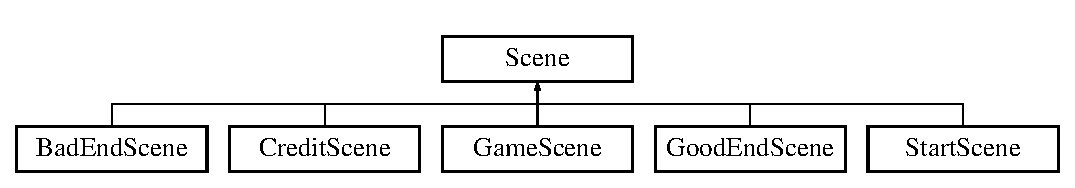
\includegraphics[height=2.000000cm]{class_scene}
\end{center}
\end{figure}
\subsection*{\-Public 멤버 함수}
\begin{DoxyCompactItemize}
\item 
virtual void \hyperlink{class_scene_abb3b6efc6fdba03cd96436edaf08a967}{init} ()
\item 
virtual void \hyperlink{class_scene_a5f8c03499f5adff28224ccaaf95a8d90}{clean\-\_\-up} ()
\item 
virtual void \hyperlink{class_scene_a280970a0176e70f76d2420c50261d6fa}{do\-\_\-event} ()
\item 
virtual void \hyperlink{class_scene_a6f447a90b1f9009acfb72df711473875}{show} ()
\item 
virtual \hyperlink{class_scene_a3b8cec2e32546713915f8c6303c951f1}{$\sim$\-Scene} ()
\end{DoxyCompactItemize}
\subsection*{\-Protected 속성}
\begin{DoxyCompactItemize}
\item 
\-S\-D\-L\-\_\-\-Surface $\ast$ \hyperlink{class_scene_a718f0a2f6a7a3290c176e3ec451f612d}{background}
\end{DoxyCompactItemize}


\subsection{생성자 \& 소멸자 문서화}
\hypertarget{class_scene_a3b8cec2e32546713915f8c6303c951f1}{\index{\-Scene@{\-Scene}!$\sim$\-Scene@{$\sim$\-Scene}}
\index{$\sim$\-Scene@{$\sim$\-Scene}!Scene@{\-Scene}}
\subsubsection[{$\sim$\-Scene}]{\setlength{\rightskip}{0pt plus 5cm}{\bf \-Scene\-::$\sim$\-Scene} (
\begin{DoxyParamCaption}
{}
\end{DoxyParamCaption}
)\hspace{0.3cm}{\ttfamily  \mbox{[}virtual\mbox{]}}}}\label{class_scene_a3b8cec2e32546713915f8c6303c951f1}


\subsection{멤버 함수 문서화}
\hypertarget{class_scene_a5f8c03499f5adff28224ccaaf95a8d90}{\index{\-Scene@{\-Scene}!clean\-\_\-up@{clean\-\_\-up}}
\index{clean\-\_\-up@{clean\-\_\-up}!Scene@{\-Scene}}
\subsubsection[{clean\-\_\-up}]{\setlength{\rightskip}{0pt plus 5cm}void {\bf \-Scene\-::clean\-\_\-up} (
\begin{DoxyParamCaption}
{}
\end{DoxyParamCaption}
)\hspace{0.3cm}{\ttfamily  \mbox{[}virtual\mbox{]}}}}\label{class_scene_a5f8c03499f5adff28224ccaaf95a8d90}


\hyperlink{class_game_scene_a1e341f7ef5fc4659ee00828ce5be753b}{\-Game\-Scene}, \hyperlink{class_credit_scene_a51294d71978f451fba4cf1c2e9617d51}{\-Credit\-Scene}, \hyperlink{class_good_end_scene_ab3d4faec409c826ee0f6a2752ac60dee}{\-Good\-End\-Scene}, \hyperlink{class_bad_end_scene_ae3dbd5c915a23f4c6ea47d57789a7545}{\-Bad\-End\-Scene}, \hyperlink{class_start_scene_a81c23a806e7d6930bf6a05837a9f819a}{\-Start\-Scene}에서 재구현되었습니다.

\hypertarget{class_scene_a280970a0176e70f76d2420c50261d6fa}{\index{\-Scene@{\-Scene}!do\-\_\-event@{do\-\_\-event}}
\index{do\-\_\-event@{do\-\_\-event}!Scene@{\-Scene}}
\subsubsection[{do\-\_\-event}]{\setlength{\rightskip}{0pt plus 5cm}void {\bf \-Scene\-::do\-\_\-event} (
\begin{DoxyParamCaption}
{}
\end{DoxyParamCaption}
)\hspace{0.3cm}{\ttfamily  \mbox{[}virtual\mbox{]}}}}\label{class_scene_a280970a0176e70f76d2420c50261d6fa}


\hyperlink{class_game_scene_add4701b7cc4649c5eee8f98ac273286a}{\-Game\-Scene}, \hyperlink{class_credit_scene_af465a04b7ec8b7f6cc157d8f86740af6}{\-Credit\-Scene}, \hyperlink{class_good_end_scene_a2015e80af48f0e7aa53dc1186dc173e9}{\-Good\-End\-Scene}, \hyperlink{class_bad_end_scene_a8dd11870a1bc9115eaf2dd02a336c492}{\-Bad\-End\-Scene}, \hyperlink{class_start_scene_a4a8c7d0442c7c9e410f69cf2368156ac}{\-Start\-Scene}에서 재구현되었습니다.

\hypertarget{class_scene_abb3b6efc6fdba03cd96436edaf08a967}{\index{\-Scene@{\-Scene}!init@{init}}
\index{init@{init}!Scene@{\-Scene}}
\subsubsection[{init}]{\setlength{\rightskip}{0pt plus 5cm}void {\bf \-Scene\-::init} (
\begin{DoxyParamCaption}
{}
\end{DoxyParamCaption}
)\hspace{0.3cm}{\ttfamily  \mbox{[}virtual\mbox{]}}}}\label{class_scene_abb3b6efc6fdba03cd96436edaf08a967}


\hyperlink{class_game_scene_ae379e50ebfc2b3cc53906e9d8a11b1d2}{\-Game\-Scene}, \hyperlink{class_credit_scene_a565f227f48dbdb61858b85f362a23d6a}{\-Credit\-Scene}, \hyperlink{class_good_end_scene_a63feec1f4ee968e29cf04a6c499360c3}{\-Good\-End\-Scene}, \hyperlink{class_bad_end_scene_a4d8802f274eaed7c1b28284505b2f8eb}{\-Bad\-End\-Scene}, \hyperlink{class_start_scene_a51b8106129b0e3332730d78900d07adb}{\-Start\-Scene}에서 재구현되었습니다.

\hypertarget{class_scene_a6f447a90b1f9009acfb72df711473875}{\index{\-Scene@{\-Scene}!show@{show}}
\index{show@{show}!Scene@{\-Scene}}
\subsubsection[{show}]{\setlength{\rightskip}{0pt plus 5cm}void {\bf \-Scene\-::show} (
\begin{DoxyParamCaption}
{}
\end{DoxyParamCaption}
)\hspace{0.3cm}{\ttfamily  \mbox{[}virtual\mbox{]}}}}\label{class_scene_a6f447a90b1f9009acfb72df711473875}


\hyperlink{class_game_scene_a17ab02461114e20f681d73a9b2528532}{\-Game\-Scene}, \hyperlink{class_credit_scene_a9a6f9d39dbdb43510295522679b20b1e}{\-Credit\-Scene}, \hyperlink{class_good_end_scene_a29207c910451e85aab64796959ad8e6d}{\-Good\-End\-Scene}, \hyperlink{class_bad_end_scene_a668bb0f3c662a5698631adaf7f3a6829}{\-Bad\-End\-Scene}, \hyperlink{class_start_scene_a79a6fe2bf885ed375be54f2ee5597e6c}{\-Start\-Scene}에서 재구현되었습니다.



\subsection{멤버 데이타 문서화}
\hypertarget{class_scene_a718f0a2f6a7a3290c176e3ec451f612d}{\index{\-Scene@{\-Scene}!background@{background}}
\index{background@{background}!Scene@{\-Scene}}
\subsubsection[{background}]{\setlength{\rightskip}{0pt plus 5cm}\-S\-D\-L\-\_\-\-Surface$\ast$ {\bf \-Scene\-::background}\hspace{0.3cm}{\ttfamily  \mbox{[}protected\mbox{]}}}}\label{class_scene_a718f0a2f6a7a3290c176e3ec451f612d}


이 클래스에 대한 문서화 페이지는 다음의 파일들로부터 생성되었습니다.\-:\begin{DoxyCompactItemize}
\item 
\hyperlink{_scene_8h}{\-Scene.\-h}\item 
\hyperlink{_scene_8cpp}{\-Scene.\-cpp}\end{DoxyCompactItemize}

\hypertarget{class_sprite}{\section{\-Sprite 클래스 참조}
\label{class_sprite}\index{\-Sprite@{\-Sprite}}
}


{\ttfamily \#include $<$sprite.\-h$>$}

\subsection*{\-Public 멤버 함수}
\begin{DoxyCompactItemize}
\item 
void \hyperlink{class_sprite_ac6cd23671a7d6aec1dd7c94680ce1da9}{sprite} ()
\end{DoxyCompactItemize}
\subsection*{\-Protected 속성}
\begin{DoxyCompactItemize}
\item 
int \hyperlink{class_sprite_abdcdaf5dc3b8842622536f318d6daac3}{frame}
\end{DoxyCompactItemize}


\subsection{멤버 함수 문서화}
\hypertarget{class_sprite_ac6cd23671a7d6aec1dd7c94680ce1da9}{\index{\-Sprite@{\-Sprite}!sprite@{sprite}}
\index{sprite@{sprite}!Sprite@{\-Sprite}}
\subsubsection[{sprite}]{\setlength{\rightskip}{0pt plus 5cm}void {\bf \-Sprite\-::sprite} (
\begin{DoxyParamCaption}
{}
\end{DoxyParamCaption}
)}}\label{class_sprite_ac6cd23671a7d6aec1dd7c94680ce1da9}


\subsection{멤버 데이타 문서화}
\hypertarget{class_sprite_abdcdaf5dc3b8842622536f318d6daac3}{\index{\-Sprite@{\-Sprite}!frame@{frame}}
\index{frame@{frame}!Sprite@{\-Sprite}}
\subsubsection[{frame}]{\setlength{\rightskip}{0pt plus 5cm}int {\bf \-Sprite\-::frame}\hspace{0.3cm}{\ttfamily  \mbox{[}protected\mbox{]}}}}\label{class_sprite_abdcdaf5dc3b8842622536f318d6daac3}


이 클래스에 대한 문서화 페이지는 다음의 파일로부터 생성되었습니다.\-:\begin{DoxyCompactItemize}
\item 
\hyperlink{sprite_8h}{sprite.\-h}\end{DoxyCompactItemize}

\hypertarget{class_start_scene}{\section{\-Start\-Scene 클래스 참조}
\label{class_start_scene}\index{\-Start\-Scene@{\-Start\-Scene}}
}


{\ttfamily \#include $<$\-Scene.\-h$>$}

\-Start\-Scene에 대한 상속 다이어그램 \-: \begin{figure}[H]
\begin{center}
\leavevmode
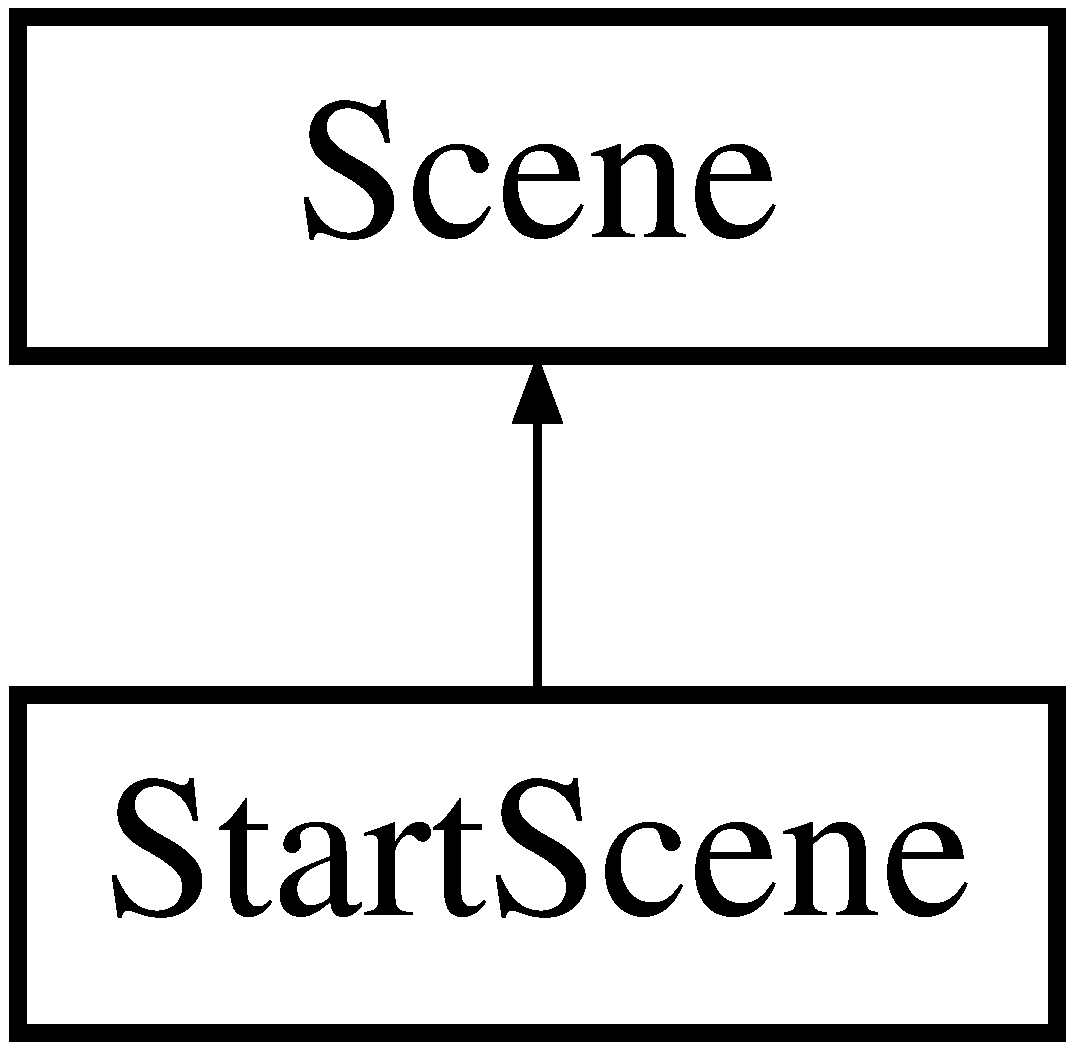
\includegraphics[height=2.000000cm]{class_start_scene}
\end{center}
\end{figure}
\subsection*{\-Public 멤버 함수}
\begin{DoxyCompactItemize}
\item 
\hyperlink{class_start_scene_abb55e5aa3fa6338d1bd21818ee1586d7}{\-Start\-Scene} ()
\item 
virtual void \hyperlink{class_start_scene_a51b8106129b0e3332730d78900d07adb}{init} ()
\item 
virtual void \hyperlink{class_start_scene_a81c23a806e7d6930bf6a05837a9f819a}{clean\-\_\-up} ()
\item 
virtual void \hyperlink{class_start_scene_a4a8c7d0442c7c9e410f69cf2368156ac}{do\-\_\-event} ()
\item 
virtual void \hyperlink{class_start_scene_a79a6fe2bf885ed375be54f2ee5597e6c}{show} ()
\end{DoxyCompactItemize}


\subsection{생성자 \& 소멸자 문서화}
\hypertarget{class_start_scene_abb55e5aa3fa6338d1bd21818ee1586d7}{\index{\-Start\-Scene@{\-Start\-Scene}!\-Start\-Scene@{\-Start\-Scene}}
\index{\-Start\-Scene@{\-Start\-Scene}!StartScene@{\-Start\-Scene}}
\subsubsection[{\-Start\-Scene}]{\setlength{\rightskip}{0pt plus 5cm}{\bf \-Start\-Scene\-::\-Start\-Scene} (
\begin{DoxyParamCaption}
{}
\end{DoxyParamCaption}
)}}\label{class_start_scene_abb55e5aa3fa6338d1bd21818ee1586d7}


\subsection{멤버 함수 문서화}
\hypertarget{class_start_scene_a81c23a806e7d6930bf6a05837a9f819a}{\index{\-Start\-Scene@{\-Start\-Scene}!clean\-\_\-up@{clean\-\_\-up}}
\index{clean\-\_\-up@{clean\-\_\-up}!StartScene@{\-Start\-Scene}}
\subsubsection[{clean\-\_\-up}]{\setlength{\rightskip}{0pt plus 5cm}void {\bf \-Start\-Scene\-::clean\-\_\-up} (
\begin{DoxyParamCaption}
{}
\end{DoxyParamCaption}
)\hspace{0.3cm}{\ttfamily  \mbox{[}virtual\mbox{]}}}}\label{class_start_scene_a81c23a806e7d6930bf6a05837a9f819a}


\hyperlink{class_scene_a5f8c03499f5adff28224ccaaf95a8d90}{\-Scene}(으)로부터 재구현되었습니다.

\hypertarget{class_start_scene_a4a8c7d0442c7c9e410f69cf2368156ac}{\index{\-Start\-Scene@{\-Start\-Scene}!do\-\_\-event@{do\-\_\-event}}
\index{do\-\_\-event@{do\-\_\-event}!StartScene@{\-Start\-Scene}}
\subsubsection[{do\-\_\-event}]{\setlength{\rightskip}{0pt plus 5cm}void {\bf \-Start\-Scene\-::do\-\_\-event} (
\begin{DoxyParamCaption}
{}
\end{DoxyParamCaption}
)\hspace{0.3cm}{\ttfamily  \mbox{[}virtual\mbox{]}}}}\label{class_start_scene_a4a8c7d0442c7c9e410f69cf2368156ac}


\hyperlink{class_scene_a280970a0176e70f76d2420c50261d6fa}{\-Scene}(으)로부터 재구현되었습니다.

\hypertarget{class_start_scene_a51b8106129b0e3332730d78900d07adb}{\index{\-Start\-Scene@{\-Start\-Scene}!init@{init}}
\index{init@{init}!StartScene@{\-Start\-Scene}}
\subsubsection[{init}]{\setlength{\rightskip}{0pt plus 5cm}void {\bf \-Start\-Scene\-::init} (
\begin{DoxyParamCaption}
{}
\end{DoxyParamCaption}
)\hspace{0.3cm}{\ttfamily  \mbox{[}virtual\mbox{]}}}}\label{class_start_scene_a51b8106129b0e3332730d78900d07adb}


\hyperlink{class_scene_abb3b6efc6fdba03cd96436edaf08a967}{\-Scene}(으)로부터 재구현되었습니다.

\hypertarget{class_start_scene_a79a6fe2bf885ed375be54f2ee5597e6c}{\index{\-Start\-Scene@{\-Start\-Scene}!show@{show}}
\index{show@{show}!StartScene@{\-Start\-Scene}}
\subsubsection[{show}]{\setlength{\rightskip}{0pt plus 5cm}void {\bf \-Start\-Scene\-::show} (
\begin{DoxyParamCaption}
{}
\end{DoxyParamCaption}
)\hspace{0.3cm}{\ttfamily  \mbox{[}virtual\mbox{]}}}}\label{class_start_scene_a79a6fe2bf885ed375be54f2ee5597e6c}


\hyperlink{class_scene_a6f447a90b1f9009acfb72df711473875}{\-Scene}(으)로부터 재구현되었습니다.



이 클래스에 대한 문서화 페이지는 다음의 파일들로부터 생성되었습니다.\-:\begin{DoxyCompactItemize}
\item 
\hyperlink{_scene_8h}{\-Scene.\-h}\item 
\hyperlink{_scene_8cpp}{\-Scene.\-cpp}\end{DoxyCompactItemize}

\hypertarget{class_timer}{\section{\-Timer 클래스 참조}
\label{class_timer}\index{\-Timer@{\-Timer}}
}


{\ttfamily \#include $<$timer.\-h$>$}

\subsection*{\-Public 멤버 함수}
\begin{DoxyCompactItemize}
\item 
\hyperlink{class_timer_a5f16e8da27d2a5a5242dead46de05d97}{\-Timer} ()
\item 
void \hyperlink{class_timer_a3a8b5272198d029779dc9302a54305a8}{start} ()
\item 
void \hyperlink{class_timer_a63f0eb44b27402196590a03781515dba}{stop} ()
\item 
void \hyperlink{class_timer_a0289effad7b573c508bc27e405900a23}{pause} ()
\item 
void \hyperlink{class_timer_aa4dd50d7ed48ac73efed2950749d35d6}{unpause} ()
\item 
int \hyperlink{class_timer_a56d411d072f1cc22b53f6ccb74cc7f63}{get\-\_\-ticks} ()
\item 
bool \hyperlink{class_timer_a8aabbd05a0fc030e7156b01bcd8264db}{is\-\_\-started} ()
\item 
bool \hyperlink{class_timer_a18c977688b4e0809cb603e9abb265950}{is\-\_\-paused} ()
\end{DoxyCompactItemize}


\subsection{생성자 \& 소멸자 문서화}
\hypertarget{class_timer_a5f16e8da27d2a5a5242dead46de05d97}{\index{\-Timer@{\-Timer}!\-Timer@{\-Timer}}
\index{\-Timer@{\-Timer}!Timer@{\-Timer}}
\subsubsection[{\-Timer}]{\setlength{\rightskip}{0pt plus 5cm}{\bf \-Timer\-::\-Timer} (
\begin{DoxyParamCaption}
{}
\end{DoxyParamCaption}
)}}\label{class_timer_a5f16e8da27d2a5a5242dead46de05d97}


\subsection{멤버 함수 문서화}
\hypertarget{class_timer_a56d411d072f1cc22b53f6ccb74cc7f63}{\index{\-Timer@{\-Timer}!get\-\_\-ticks@{get\-\_\-ticks}}
\index{get\-\_\-ticks@{get\-\_\-ticks}!Timer@{\-Timer}}
\subsubsection[{get\-\_\-ticks}]{\setlength{\rightskip}{0pt plus 5cm}int {\bf \-Timer\-::get\-\_\-ticks} (
\begin{DoxyParamCaption}
{}
\end{DoxyParamCaption}
)}}\label{class_timer_a56d411d072f1cc22b53f6ccb74cc7f63}
\hypertarget{class_timer_a18c977688b4e0809cb603e9abb265950}{\index{\-Timer@{\-Timer}!is\-\_\-paused@{is\-\_\-paused}}
\index{is\-\_\-paused@{is\-\_\-paused}!Timer@{\-Timer}}
\subsubsection[{is\-\_\-paused}]{\setlength{\rightskip}{0pt plus 5cm}bool {\bf \-Timer\-::is\-\_\-paused} (
\begin{DoxyParamCaption}
{}
\end{DoxyParamCaption}
)}}\label{class_timer_a18c977688b4e0809cb603e9abb265950}
\hypertarget{class_timer_a8aabbd05a0fc030e7156b01bcd8264db}{\index{\-Timer@{\-Timer}!is\-\_\-started@{is\-\_\-started}}
\index{is\-\_\-started@{is\-\_\-started}!Timer@{\-Timer}}
\subsubsection[{is\-\_\-started}]{\setlength{\rightskip}{0pt plus 5cm}bool {\bf \-Timer\-::is\-\_\-started} (
\begin{DoxyParamCaption}
{}
\end{DoxyParamCaption}
)}}\label{class_timer_a8aabbd05a0fc030e7156b01bcd8264db}
\hypertarget{class_timer_a0289effad7b573c508bc27e405900a23}{\index{\-Timer@{\-Timer}!pause@{pause}}
\index{pause@{pause}!Timer@{\-Timer}}
\subsubsection[{pause}]{\setlength{\rightskip}{0pt plus 5cm}void {\bf \-Timer\-::pause} (
\begin{DoxyParamCaption}
{}
\end{DoxyParamCaption}
)}}\label{class_timer_a0289effad7b573c508bc27e405900a23}
\hypertarget{class_timer_a3a8b5272198d029779dc9302a54305a8}{\index{\-Timer@{\-Timer}!start@{start}}
\index{start@{start}!Timer@{\-Timer}}
\subsubsection[{start}]{\setlength{\rightskip}{0pt plus 5cm}void {\bf \-Timer\-::start} (
\begin{DoxyParamCaption}
{}
\end{DoxyParamCaption}
)}}\label{class_timer_a3a8b5272198d029779dc9302a54305a8}
\hypertarget{class_timer_a63f0eb44b27402196590a03781515dba}{\index{\-Timer@{\-Timer}!stop@{stop}}
\index{stop@{stop}!Timer@{\-Timer}}
\subsubsection[{stop}]{\setlength{\rightskip}{0pt plus 5cm}void {\bf \-Timer\-::stop} (
\begin{DoxyParamCaption}
{}
\end{DoxyParamCaption}
)}}\label{class_timer_a63f0eb44b27402196590a03781515dba}
\hypertarget{class_timer_aa4dd50d7ed48ac73efed2950749d35d6}{\index{\-Timer@{\-Timer}!unpause@{unpause}}
\index{unpause@{unpause}!Timer@{\-Timer}}
\subsubsection[{unpause}]{\setlength{\rightskip}{0pt plus 5cm}void {\bf \-Timer\-::unpause} (
\begin{DoxyParamCaption}
{}
\end{DoxyParamCaption}
)}}\label{class_timer_aa4dd50d7ed48ac73efed2950749d35d6}


이 클래스에 대한 문서화 페이지는 다음의 파일들로부터 생성되었습니다.\-:\begin{DoxyCompactItemize}
\item 
\hyperlink{timer_8h}{timer.\-h}\item 
\hyperlink{_timer_8cpp}{\-Timer.\-cpp}\end{DoxyCompactItemize}

\hypertarget{class_top}{\section{\-Top 클래스 참조}
\label{class_top}\index{\-Top@{\-Top}}
}


{\ttfamily \#include $<$\-Scene.\-h$>$}

\subsection*{\-Public 멤버 함수}
\begin{DoxyCompactItemize}
\item 
\hyperlink{class_top_a46b55aaac1bb900d88b11fa662c4f886}{\-Top} (int x, int y, int w, int h)
\item 
void \hyperlink{class_top_a80f068054b19da8ea9afb9705ccc524d}{show} (\-S\-D\-L\-\_\-\-Surface $\ast$)
\item 
void \hyperlink{class_top_aa951de118eb232ce100d787082d6ca03}{set\-\_\-credit\-\_\-score} (int credit)
\item 
void \hyperlink{class_top_aaff6dac540f22b04173e2d6a5f8e3cb7}{set\-\_\-total\-\_\-dept} (int total)
\end{DoxyCompactItemize}


\subsection{생성자 \& 소멸자 문서화}
\hypertarget{class_top_a46b55aaac1bb900d88b11fa662c4f886}{\index{\-Top@{\-Top}!\-Top@{\-Top}}
\index{\-Top@{\-Top}!Top@{\-Top}}
\subsubsection[{\-Top}]{\setlength{\rightskip}{0pt plus 5cm}{\bf \-Top\-::\-Top} (
\begin{DoxyParamCaption}
\item[{int}]{x, }
\item[{int}]{y, }
\item[{int}]{w, }
\item[{int}]{h}
\end{DoxyParamCaption}
)}}\label{class_top_a46b55aaac1bb900d88b11fa662c4f886}


\subsection{멤버 함수 문서화}
\hypertarget{class_top_aa951de118eb232ce100d787082d6ca03}{\index{\-Top@{\-Top}!set\-\_\-credit\-\_\-score@{set\-\_\-credit\-\_\-score}}
\index{set\-\_\-credit\-\_\-score@{set\-\_\-credit\-\_\-score}!Top@{\-Top}}
\subsubsection[{set\-\_\-credit\-\_\-score}]{\setlength{\rightskip}{0pt plus 5cm}void {\bf \-Top\-::set\-\_\-credit\-\_\-score} (
\begin{DoxyParamCaption}
\item[{int}]{credit}
\end{DoxyParamCaption}
)}}\label{class_top_aa951de118eb232ce100d787082d6ca03}
\hypertarget{class_top_aaff6dac540f22b04173e2d6a5f8e3cb7}{\index{\-Top@{\-Top}!set\-\_\-total\-\_\-dept@{set\-\_\-total\-\_\-dept}}
\index{set\-\_\-total\-\_\-dept@{set\-\_\-total\-\_\-dept}!Top@{\-Top}}
\subsubsection[{set\-\_\-total\-\_\-dept}]{\setlength{\rightskip}{0pt plus 5cm}void {\bf \-Top\-::set\-\_\-total\-\_\-dept} (
\begin{DoxyParamCaption}
\item[{int}]{total}
\end{DoxyParamCaption}
)}}\label{class_top_aaff6dac540f22b04173e2d6a5f8e3cb7}
\hypertarget{class_top_a80f068054b19da8ea9afb9705ccc524d}{\index{\-Top@{\-Top}!show@{show}}
\index{show@{show}!Top@{\-Top}}
\subsubsection[{show}]{\setlength{\rightskip}{0pt plus 5cm}void {\bf \-Top\-::show} (
\begin{DoxyParamCaption}
\item[{\-S\-D\-L\-\_\-\-Surface $\ast$}]{background}
\end{DoxyParamCaption}
)}}\label{class_top_a80f068054b19da8ea9afb9705ccc524d}


이 클래스에 대한 문서화 페이지는 다음의 파일들로부터 생성되었습니다.\-:\begin{DoxyCompactItemize}
\item 
\hyperlink{_scene_8h}{\-Scene.\-h}\item 
\hyperlink{_game_scene___g_u_i_8cpp}{\-Game\-Scene\-\_\-\-G\-U\-I.\-cpp}\end{DoxyCompactItemize}

\hypertarget{class_wallet_bar}{\section{\-Wallet\-Bar 클래스 참조}
\label{class_wallet_bar}\index{\-Wallet\-Bar@{\-Wallet\-Bar}}
}


{\ttfamily \#include $<$\-Scene.\-h$>$}

\subsection*{\-Public 멤버 함수}
\begin{DoxyCompactItemize}
\item 
void \hyperlink{class_wallet_bar_a0e06514afd3b4f67b4b84c42f8d660b2}{init} (int x, int y, int w, int h)
\item 
void \hyperlink{class_wallet_bar_a5f41d329128d28f73a8c1c8dadae3eb7}{clean\-\_\-up} ()
\item 
void \hyperlink{class_wallet_bar_a28e4d7b035ef6ac5aff8db6b0350bc9c}{show} ()
\item 
void \hyperlink{class_wallet_bar_ade5b8ead100246a0b8da4fba1fc3ffc8}{print\-\_\-limit} (\hyperlink{_constants_8h_a03f7ec9e12b891db1bbeda07eb4099d7}{\-E\-Card}, uint64\-\_\-t)
\item 
void \hyperlink{class_wallet_bar_a9be459da1602fe0432ca83d92a20faf5}{show\-\_\-gage} (\hyperlink{_constants_8h_a03f7ec9e12b891db1bbeda07eb4099d7}{\-E\-Card}, float)
\end{DoxyCompactItemize}


\subsection{멤버 함수 문서화}
\hypertarget{class_wallet_bar_a5f41d329128d28f73a8c1c8dadae3eb7}{\index{\-Wallet\-Bar@{\-Wallet\-Bar}!clean\-\_\-up@{clean\-\_\-up}}
\index{clean\-\_\-up@{clean\-\_\-up}!WalletBar@{\-Wallet\-Bar}}
\subsubsection[{clean\-\_\-up}]{\setlength{\rightskip}{0pt plus 5cm}void {\bf \-Wallet\-Bar\-::clean\-\_\-up} (
\begin{DoxyParamCaption}
{}
\end{DoxyParamCaption}
)}}\label{class_wallet_bar_a5f41d329128d28f73a8c1c8dadae3eb7}
\hypertarget{class_wallet_bar_a0e06514afd3b4f67b4b84c42f8d660b2}{\index{\-Wallet\-Bar@{\-Wallet\-Bar}!init@{init}}
\index{init@{init}!WalletBar@{\-Wallet\-Bar}}
\subsubsection[{init}]{\setlength{\rightskip}{0pt plus 5cm}void {\bf \-Wallet\-Bar\-::init} (
\begin{DoxyParamCaption}
\item[{int}]{x, }
\item[{int}]{y, }
\item[{int}]{w, }
\item[{int}]{h}
\end{DoxyParamCaption}
)}}\label{class_wallet_bar_a0e06514afd3b4f67b4b84c42f8d660b2}
\hypertarget{class_wallet_bar_ade5b8ead100246a0b8da4fba1fc3ffc8}{\index{\-Wallet\-Bar@{\-Wallet\-Bar}!print\-\_\-limit@{print\-\_\-limit}}
\index{print\-\_\-limit@{print\-\_\-limit}!WalletBar@{\-Wallet\-Bar}}
\subsubsection[{print\-\_\-limit}]{\setlength{\rightskip}{0pt plus 5cm}void {\bf \-Wallet\-Bar\-::print\-\_\-limit} (
\begin{DoxyParamCaption}
\item[{{\bf \-E\-Card}}]{i, }
\item[{uint64\-\_\-t}]{money}
\end{DoxyParamCaption}
)}}\label{class_wallet_bar_ade5b8ead100246a0b8da4fba1fc3ffc8}
\hypertarget{class_wallet_bar_a28e4d7b035ef6ac5aff8db6b0350bc9c}{\index{\-Wallet\-Bar@{\-Wallet\-Bar}!show@{show}}
\index{show@{show}!WalletBar@{\-Wallet\-Bar}}
\subsubsection[{show}]{\setlength{\rightskip}{0pt plus 5cm}void {\bf \-Wallet\-Bar\-::show} (
\begin{DoxyParamCaption}
{}
\end{DoxyParamCaption}
)}}\label{class_wallet_bar_a28e4d7b035ef6ac5aff8db6b0350bc9c}
\hypertarget{class_wallet_bar_a9be459da1602fe0432ca83d92a20faf5}{\index{\-Wallet\-Bar@{\-Wallet\-Bar}!show\-\_\-gage@{show\-\_\-gage}}
\index{show\-\_\-gage@{show\-\_\-gage}!WalletBar@{\-Wallet\-Bar}}
\subsubsection[{show\-\_\-gage}]{\setlength{\rightskip}{0pt plus 5cm}void {\bf \-Wallet\-Bar\-::show\-\_\-gage} (
\begin{DoxyParamCaption}
\item[{{\bf \-E\-Card}}]{i, }
\item[{float}]{ratio}
\end{DoxyParamCaption}
)}}\label{class_wallet_bar_a9be459da1602fe0432ca83d92a20faf5}


이 클래스에 대한 문서화 페이지는 다음의 파일들로부터 생성되었습니다.\-:\begin{DoxyCompactItemize}
\item 
\hyperlink{_scene_8h}{\-Scene.\-h}\item 
\hyperlink{_game_scene___g_u_i_8cpp}{\-Game\-Scene\-\_\-\-G\-U\-I.\-cpp}\end{DoxyCompactItemize}

\chapter{파일 문서화}
\hypertarget{building_8cpp}{\section{building.\-cpp 파일 참조}
\label{building_8cpp}\index{building.\-cpp@{building.\-cpp}}
}
{\ttfamily \#include \char`\"{}building.\-h\char`\"{}}\*
{\ttfamily \#include \char`\"{}global.\-h\char`\"{}}\*
{\ttfamily \#include \char`\"{}\-Configuration.\-h\char`\"{}}\*

\hypertarget{building_8h}{\section{building.\-h 파일 참조}
\label{building_8h}\index{building.\-h@{building.\-h}}
}
{\ttfamily \#include \char`\"{}common.\-h\char`\"{}}\*
{\ttfamily \#include \char`\"{}collider.\-h\char`\"{}}\*
{\ttfamily \#include \char`\"{}global.\-h\char`\"{}}\*
{\ttfamily \#include \char`\"{}\-Constants.\-h\char`\"{}}\*
\subsection*{클래스}
\begin{DoxyCompactItemize}
\item 
class \hyperlink{class_door}{\-Door}
\item 
class \hyperlink{class_building}{\-Building}
\end{DoxyCompactItemize}

\hypertarget{_card_8cpp}{\section{\-Card.\-cpp 파일 참조}
\label{_card_8cpp}\index{\-Card.\-cpp@{\-Card.\-cpp}}
}
{\ttfamily \#include \char`\"{}\-Card.\-h\char`\"{}}\*

\hypertarget{_card_8h}{\section{\-Card.\-h 파일 참조}
\label{_card_8h}\index{\-Card.\-h@{\-Card.\-h}}
}
{\ttfamily \#include $<$string$>$}\*
{\ttfamily \#include $<$sstream$>$}\*
\subsection*{클래스}
\begin{DoxyCompactItemize}
\item 
class \hyperlink{class_card}{\-Card}
\end{DoxyCompactItemize}

\hypertarget{_c_card_8cpp}{\section{\-C\-Card.\-cpp 파일 참조}
\label{_c_card_8cpp}\index{\-C\-Card.\-cpp@{\-C\-Card.\-cpp}}
}
{\ttfamily \#include \char`\"{}\-C\-Card.\-h\char`\"{}}\*

\hypertarget{_c_card_8h}{\section{\-C\-Card.\-h 파일 참조}
\label{_c_card_8h}\index{\-C\-Card.\-h@{\-C\-Card.\-h}}
}
{\ttfamily \#include $<$stdint.\-h$>$}\*
{\ttfamily \#include \char`\"{}\-Constants.\-h\char`\"{}}\*
{\ttfamily \#include \char`\"{}\-Global\-Functions.\-h\char`\"{}}\*
\subsection*{클래스}
\begin{DoxyCompactItemize}
\item 
class \hyperlink{class_c_card}{\-C\-Card}
\end{DoxyCompactItemize}

\hypertarget{character_8cpp}{\section{character.\-cpp 파일 참조}
\label{character_8cpp}\index{character.\-cpp@{character.\-cpp}}
}
{\ttfamily \#include \char`\"{}global.\-h\char`\"{}}\*
{\ttfamily \#include \char`\"{}\-Configuration.\-h\char`\"{}}\*
{\ttfamily \#include \char`\"{}common.\-h\char`\"{}}\*
{\ttfamily \#include \char`\"{}character.\-h\char`\"{}}\*
{\ttfamily \#include $<$stdint.\-h$>$}\*

\hypertarget{character_8h}{\section{character.\-h 파일 참조}
\label{character_8h}\index{character.\-h@{character.\-h}}
}
{\ttfamily \#include \char`\"{}common.\-h\char`\"{}}\*
{\ttfamily \#include \char`\"{}collider.\-h\char`\"{}}\*
{\ttfamily \#include \char`\"{}\-C\-Player.\-h\char`\"{}}\*
{\ttfamily \#include \char`\"{}\-Constants.\-h\char`\"{}}\*
\subsection*{클래스}
\begin{DoxyCompactItemize}
\item 
class \hyperlink{class_character}{\-Character}
\item 
class \hyperlink{class_hero}{\-Hero}
\item 
class \hyperlink{class_gang}{\-Gang}
\end{DoxyCompactItemize}
\subsection*{매크로}
\begin{DoxyCompactItemize}
\item 
\#define \hyperlink{character_8h_a0f44a1e28bd1be64ec9cec79733ea098}{\-\_\-\-M\-E\-J\-E\-C\-T\-Y\-\_\-\-C\-H\-A\-R\-\_\-\-H\-\_\-\-\_\-}
\end{DoxyCompactItemize}
\subsection*{변수}
\begin{DoxyCompactItemize}
\item 
const int \hyperlink{character_8h_a434e4725f04fa366ed1341f04d38521d}{\-D\-O\-W\-N} = 0
\item 
const int \hyperlink{character_8h_a08e9e19b88c4004c6d1daa0ed765c569}{\-L\-E\-F\-T} = 1
\item 
const int \hyperlink{character_8h_a088fe0153a918af361dc8f4e775d020e}{\-R\-I\-G\-H\-T} = 2
\item 
const int \hyperlink{character_8h_ac58327b7b857c0d4c71c07aa602ace58}{\-U\-P} = 3
\item 
const int \hyperlink{character_8h_adfabeb87d2932b78a358704bacae0891}{\-S\-T\-O\-P} = 4
\end{DoxyCompactItemize}


\subsection{매크로 문서화}
\hypertarget{character_8h_a0f44a1e28bd1be64ec9cec79733ea098}{\index{character.\-h@{character.\-h}!\-\_\-\-M\-E\-J\-E\-C\-T\-Y\-\_\-\-C\-H\-A\-R\-\_\-\-H\-\_\-\-\_\-@{\-\_\-\-M\-E\-J\-E\-C\-T\-Y\-\_\-\-C\-H\-A\-R\-\_\-\-H\-\_\-\-\_\-}}
\index{\-\_\-\-M\-E\-J\-E\-C\-T\-Y\-\_\-\-C\-H\-A\-R\-\_\-\-H\-\_\-\-\_\-@{\-\_\-\-M\-E\-J\-E\-C\-T\-Y\-\_\-\-C\-H\-A\-R\-\_\-\-H\-\_\-\-\_\-}!character.h@{character.\-h}}
\subsubsection[{\-\_\-\-M\-E\-J\-E\-C\-T\-Y\-\_\-\-C\-H\-A\-R\-\_\-\-H\-\_\-\-\_\-}]{\setlength{\rightskip}{0pt plus 5cm}\#define {\bf \-\_\-\-M\-E\-J\-E\-C\-T\-Y\-\_\-\-C\-H\-A\-R\-\_\-\-H\-\_\-\-\_\-}}}\label{character_8h_a0f44a1e28bd1be64ec9cec79733ea098}


\subsection{변수 문서화}
\hypertarget{character_8h_a434e4725f04fa366ed1341f04d38521d}{\index{character.\-h@{character.\-h}!\-D\-O\-W\-N@{\-D\-O\-W\-N}}
\index{\-D\-O\-W\-N@{\-D\-O\-W\-N}!character.h@{character.\-h}}
\subsubsection[{\-D\-O\-W\-N}]{\setlength{\rightskip}{0pt plus 5cm}const int {\bf \-D\-O\-W\-N} = 0}}\label{character_8h_a434e4725f04fa366ed1341f04d38521d}
\hypertarget{character_8h_a08e9e19b88c4004c6d1daa0ed765c569}{\index{character.\-h@{character.\-h}!\-L\-E\-F\-T@{\-L\-E\-F\-T}}
\index{\-L\-E\-F\-T@{\-L\-E\-F\-T}!character.h@{character.\-h}}
\subsubsection[{\-L\-E\-F\-T}]{\setlength{\rightskip}{0pt plus 5cm}const int {\bf \-L\-E\-F\-T} = 1}}\label{character_8h_a08e9e19b88c4004c6d1daa0ed765c569}
\hypertarget{character_8h_a088fe0153a918af361dc8f4e775d020e}{\index{character.\-h@{character.\-h}!\-R\-I\-G\-H\-T@{\-R\-I\-G\-H\-T}}
\index{\-R\-I\-G\-H\-T@{\-R\-I\-G\-H\-T}!character.h@{character.\-h}}
\subsubsection[{\-R\-I\-G\-H\-T}]{\setlength{\rightskip}{0pt plus 5cm}const int {\bf \-R\-I\-G\-H\-T} = 2}}\label{character_8h_a088fe0153a918af361dc8f4e775d020e}
\hypertarget{character_8h_adfabeb87d2932b78a358704bacae0891}{\index{character.\-h@{character.\-h}!\-S\-T\-O\-P@{\-S\-T\-O\-P}}
\index{\-S\-T\-O\-P@{\-S\-T\-O\-P}!character.h@{character.\-h}}
\subsubsection[{\-S\-T\-O\-P}]{\setlength{\rightskip}{0pt plus 5cm}const int {\bf \-S\-T\-O\-P} = 4}}\label{character_8h_adfabeb87d2932b78a358704bacae0891}
\hypertarget{character_8h_ac58327b7b857c0d4c71c07aa602ace58}{\index{character.\-h@{character.\-h}!\-U\-P@{\-U\-P}}
\index{\-U\-P@{\-U\-P}!character.h@{character.\-h}}
\subsubsection[{\-U\-P}]{\setlength{\rightskip}{0pt plus 5cm}const int {\bf \-U\-P} = 3}}\label{character_8h_ac58327b7b857c0d4c71c07aa602ace58}

\hypertarget{collider_8cpp}{\section{collider.\-cpp 파일 참조}
\label{collider_8cpp}\index{collider.\-cpp@{collider.\-cpp}}
}
{\ttfamily \#include \char`\"{}collider.\-h\char`\"{}}\*
\subsection*{함수}
\begin{DoxyCompactItemize}
\item 
bool \hyperlink{collider_8cpp_a574b9198f07374b0d4c5af04af56f78e}{check\-\_\-collider} (\hyperlink{class_collider}{\-Collider} $\ast$other)
\item 
\-S\-D\-L\-\_\-\-Rect $\ast$ \hyperlink{collider_8cpp_afa8b77967f73dd365e56e5e7713fae36}{get\-\_\-box} ()
\end{DoxyCompactItemize}


\subsection{함수 문서화}
\hypertarget{collider_8cpp_a574b9198f07374b0d4c5af04af56f78e}{\index{collider.\-cpp@{collider.\-cpp}!check\-\_\-collider@{check\-\_\-collider}}
\index{check\-\_\-collider@{check\-\_\-collider}!collider.cpp@{collider.\-cpp}}
\subsubsection[{check\-\_\-collider}]{\setlength{\rightskip}{0pt plus 5cm}bool {\bf check\-\_\-collider} (
\begin{DoxyParamCaption}
\item[{{\bf \-Collider} $\ast$}]{other}
\end{DoxyParamCaption}
)}}\label{collider_8cpp_a574b9198f07374b0d4c5af04af56f78e}
\hypertarget{collider_8cpp_afa8b77967f73dd365e56e5e7713fae36}{\index{collider.\-cpp@{collider.\-cpp}!get\-\_\-box@{get\-\_\-box}}
\index{get\-\_\-box@{get\-\_\-box}!collider.cpp@{collider.\-cpp}}
\subsubsection[{get\-\_\-box}]{\setlength{\rightskip}{0pt plus 5cm}\-S\-D\-L\-\_\-\-Rect$\ast$ {\bf get\-\_\-box} (
\begin{DoxyParamCaption}
{}
\end{DoxyParamCaption}
)}}\label{collider_8cpp_afa8b77967f73dd365e56e5e7713fae36}

\hypertarget{collider_8h}{\section{collider.\-h 파일 참조}
\label{collider_8h}\index{collider.\-h@{collider.\-h}}
}
{\ttfamily \#include \char`\"{}common.\-h\char`\"{}}\*
\subsection*{클래스}
\begin{DoxyCompactItemize}
\item 
class \hyperlink{class_collider}{\-Collider}
\end{DoxyCompactItemize}

\hypertarget{common_8h}{\section{common.\-h 파일 참조}
\label{common_8h}\index{common.\-h@{common.\-h}}
}
{\ttfamily \#include \char`\"{}lua/lua.\-h\char`\"{}}\*
{\ttfamily \#include \char`\"{}lua/lauxlib.\-h\char`\"{}}\*
{\ttfamily \#include \char`\"{}lua/luaconf.\-h\char`\"{}}\*
{\ttfamily \#include \char`\"{}lua/lualib.\-h\char`\"{}}\*
{\ttfamily \#include \char`\"{}\-S\-D\-L/\-S\-D\-L.\-h\char`\"{}}\*
{\ttfamily \#include \char`\"{}\-S\-D\-L/\-S\-D\-L\-\_\-image.\-h\char`\"{}}\*
{\ttfamily \#include \char`\"{}\-S\-D\-L/\-S\-D\-L\-\_\-ttf.\-h\char`\"{}}\*
{\ttfamily \#include \char`\"{}\-Constants.\-h\char`\"{}}\*
{\ttfamily \#include \char`\"{}\-Global\-Functions.\-h\char`\"{}}\*
{\ttfamily \#include \char`\"{}\-Configuration.\-h\char`\"{}}\*
{\ttfamily \#include \char`\"{}global.\-h\char`\"{}}\*
{\ttfamily \#include $<$string$>$}\*
{\ttfamily \#include $<$sstream$>$}\*
{\ttfamily \#include $<$iostream$>$}\*
{\ttfamily \#include $<$stdarg.\-h$>$}\*
\subsection*{매크로}
\begin{DoxyCompactItemize}
\item 
\#define \hyperlink{common_8h_a57f592e69956624c719715cde79ba958}{\-Zero\-Memory}(\-Destination, length)
\item 
\#define \hyperlink{common_8h_a47c1b39adb45ac8d69be4817fd2a7fc9}{\-S\-T\-R\-I\-N\-G\-I\-F\-Y}(in)~\#in
\item 
\#define \hyperlink{common_8h_abf9698ecc3d25eed8464247a96718d81}{\-M\-A\-C\-R\-O\-T\-O\-S\-T\-R\-I\-N\-G}(in)~\hyperlink{common_8h_a47c1b39adb45ac8d69be4817fd2a7fc9}{\-S\-T\-R\-I\-N\-G\-I\-F\-Y}(in)
\item 
\#define \hyperlink{common_8h_ad37a804df2a1060b453ce07fe0ee3cbc}{\-A\-T}~\-\_\-\-\_\-\-F\-I\-L\-E\-\_\-\-\_\- \char`\"{}\-:\char`\"{} \hyperlink{common_8h_abf9698ecc3d25eed8464247a96718d81}{\-M\-A\-C\-R\-O\-T\-O\-S\-T\-R\-I\-N\-G}(\-\_\-\-\_\-\-L\-I\-N\-E\-\_\-\-\_\-)
\end{DoxyCompactItemize}


\subsection{매크로 문서화}
\hypertarget{common_8h_ad37a804df2a1060b453ce07fe0ee3cbc}{\index{common.\-h@{common.\-h}!\-A\-T@{\-A\-T}}
\index{\-A\-T@{\-A\-T}!common.h@{common.\-h}}
\subsubsection[{\-A\-T}]{\setlength{\rightskip}{0pt plus 5cm}\#define {\bf \-A\-T}~\-\_\-\-\_\-\-F\-I\-L\-E\-\_\-\-\_\- \char`\"{}\-:\char`\"{} {\bf \-M\-A\-C\-R\-O\-T\-O\-S\-T\-R\-I\-N\-G}(\-\_\-\-\_\-\-L\-I\-N\-E\-\_\-\-\_\-)}}\label{common_8h_ad37a804df2a1060b453ce07fe0ee3cbc}
\hypertarget{common_8h_abf9698ecc3d25eed8464247a96718d81}{\index{common.\-h@{common.\-h}!\-M\-A\-C\-R\-O\-T\-O\-S\-T\-R\-I\-N\-G@{\-M\-A\-C\-R\-O\-T\-O\-S\-T\-R\-I\-N\-G}}
\index{\-M\-A\-C\-R\-O\-T\-O\-S\-T\-R\-I\-N\-G@{\-M\-A\-C\-R\-O\-T\-O\-S\-T\-R\-I\-N\-G}!common.h@{common.\-h}}
\subsubsection[{\-M\-A\-C\-R\-O\-T\-O\-S\-T\-R\-I\-N\-G}]{\setlength{\rightskip}{0pt plus 5cm}\#define {\bf \-M\-A\-C\-R\-O\-T\-O\-S\-T\-R\-I\-N\-G}(
\begin{DoxyParamCaption}
\item[{}]{in}
\end{DoxyParamCaption}
)~{\bf \-S\-T\-R\-I\-N\-G\-I\-F\-Y}(in)}}\label{common_8h_abf9698ecc3d25eed8464247a96718d81}
\hypertarget{common_8h_a47c1b39adb45ac8d69be4817fd2a7fc9}{\index{common.\-h@{common.\-h}!\-S\-T\-R\-I\-N\-G\-I\-F\-Y@{\-S\-T\-R\-I\-N\-G\-I\-F\-Y}}
\index{\-S\-T\-R\-I\-N\-G\-I\-F\-Y@{\-S\-T\-R\-I\-N\-G\-I\-F\-Y}!common.h@{common.\-h}}
\subsubsection[{\-S\-T\-R\-I\-N\-G\-I\-F\-Y}]{\setlength{\rightskip}{0pt plus 5cm}\#define {\bf \-S\-T\-R\-I\-N\-G\-I\-F\-Y}(
\begin{DoxyParamCaption}
\item[{}]{in}
\end{DoxyParamCaption}
)~\#in}}\label{common_8h_a47c1b39adb45ac8d69be4817fd2a7fc9}
\hypertarget{common_8h_a57f592e69956624c719715cde79ba958}{\index{common.\-h@{common.\-h}!\-Zero\-Memory@{\-Zero\-Memory}}
\index{\-Zero\-Memory@{\-Zero\-Memory}!common.h@{common.\-h}}
\subsubsection[{\-Zero\-Memory}]{\setlength{\rightskip}{0pt plus 5cm}\#define {\bf \-Zero\-Memory}(
\begin{DoxyParamCaption}
\item[{}]{\-Destination, }
\item[{}]{length}
\end{DoxyParamCaption}
)}}\label{common_8h_a57f592e69956624c719715cde79ba958}
{\bfseries 값\-:}
\begin{DoxyCode}
{ \
  memset((void*)Destination, 0, length);\
}
\end{DoxyCode}

\hypertarget{_configuration_8h}{\section{\-Configuration.\-h 파일 참조}
\label{_configuration_8h}\index{\-Configuration.\-h@{\-Configuration.\-h}}
}
\subsection*{변수}
\begin{DoxyCompactItemize}
\item 
const int \hyperlink{_configuration_8h_a3482785bd2a4c8b307f9e0b6f54e2c36}{\-S\-C\-R\-E\-E\-N\-\_\-\-W\-I\-D\-T\-H} = 640
\item 
const int \hyperlink{_configuration_8h_ab454541ae58bcf6555e8d723b1eb95e7}{\-S\-C\-R\-E\-E\-N\-\_\-\-H\-E\-I\-G\-H\-T} = 480
\item 
const int \hyperlink{_configuration_8h_a8194731fdeea643e725e3a89d2f7ec59}{\-S\-C\-R\-E\-E\-N\-\_\-\-B\-P\-P} = 32
\item 
const int \hyperlink{_configuration_8h_a74c0aab6b42576716415a4ae62282acf}{\-B\-A\-R\-\_\-\-W\-I\-D\-T\-H} = 150
\item 
const int \hyperlink{_configuration_8h_acc34e9f02552732321a45df5fbc42f98}{\-B\-A\-R\-\_\-\-H\-E\-I\-G\-H\-T} = \hyperlink{_configuration_8h_ab454541ae58bcf6555e8d723b1eb95e7}{\-S\-C\-R\-E\-E\-N\-\_\-\-H\-E\-I\-G\-H\-T}
\item 
const int \hyperlink{_configuration_8h_a6764b1b85983649f116cecddaa62535a}{\-M\-A\-P\-\_\-\-W\-I\-D\-T\-H} = 490
\item 
const int \hyperlink{_configuration_8h_a172ffb38f672960e8390ef70664d967b}{\-M\-A\-P\-\_\-\-H\-E\-I\-G\-H\-T} = \hyperlink{_configuration_8h_ab454541ae58bcf6555e8d723b1eb95e7}{\-S\-C\-R\-E\-E\-N\-\_\-\-H\-E\-I\-G\-H\-T}
\item 
const int \hyperlink{_configuration_8h_acd7dc9ec163b370b106e7250a6865e89}{\-C\-H\-A\-R\-\_\-\-V\-E\-L\-O\-C\-I\-T\-Y} = 15
\item 
bool \hyperlink{_configuration_8h_adfc9868edcb3523256495d5a53eaa358}{\-I\-S\-\_\-\-F\-U\-L\-L\-\_\-\-S\-C\-R\-E\-E\-N}
\item 
int \hyperlink{_configuration_8h_a33ca3372e33da34564fef70d2c2ccf47}{\-D\-E\-F\-A\-U\-L\-T\-\_\-\-F\-R\-A\-M\-E\-\_\-\-R\-A\-T\-E}
\item 
double \hyperlink{_configuration_8h_a197c17e106445c844080b42846f8906d}{\-D\-E\-F\-A\-U\-L\-T\-\_\-\-R\-A\-T\-E}
\item 
double \hyperlink{_configuration_8h_a856e3296ab07af6a419c7248b701897a}{\-R\-A\-T\-E\-\_\-\-R\-A\-T\-E}
\item 
int \hyperlink{_configuration_8h_a91e674bbf5c97202d30695e306ef1f7a}{\-D\-E\-F\-A\-U\-L\-T\-\_\-\-L\-I\-M\-I\-T}
\item 
int \hyperlink{_configuration_8h_af72a0cc37a1bab73a16a07bdc92c9cec}{\-L\-I\-M\-I\-T\-\_\-\-R\-A\-T\-E}
\item 
int \hyperlink{_configuration_8h_a4b64ce0da17c64a5f50eea89f4aa7ed9}{\-S\-T\-A\-R\-T\-\_\-\-G\-R\-A\-D\-E}
\end{DoxyCompactItemize}


\subsection{변수 문서화}
\hypertarget{_configuration_8h_acc34e9f02552732321a45df5fbc42f98}{\index{\-Configuration.\-h@{\-Configuration.\-h}!\-B\-A\-R\-\_\-\-H\-E\-I\-G\-H\-T@{\-B\-A\-R\-\_\-\-H\-E\-I\-G\-H\-T}}
\index{\-B\-A\-R\-\_\-\-H\-E\-I\-G\-H\-T@{\-B\-A\-R\-\_\-\-H\-E\-I\-G\-H\-T}!Configuration.h@{\-Configuration.\-h}}
\subsubsection[{\-B\-A\-R\-\_\-\-H\-E\-I\-G\-H\-T}]{\setlength{\rightskip}{0pt plus 5cm}const int {\bf \-B\-A\-R\-\_\-\-H\-E\-I\-G\-H\-T} = {\bf \-S\-C\-R\-E\-E\-N\-\_\-\-H\-E\-I\-G\-H\-T}}}\label{_configuration_8h_acc34e9f02552732321a45df5fbc42f98}
\hypertarget{_configuration_8h_a74c0aab6b42576716415a4ae62282acf}{\index{\-Configuration.\-h@{\-Configuration.\-h}!\-B\-A\-R\-\_\-\-W\-I\-D\-T\-H@{\-B\-A\-R\-\_\-\-W\-I\-D\-T\-H}}
\index{\-B\-A\-R\-\_\-\-W\-I\-D\-T\-H@{\-B\-A\-R\-\_\-\-W\-I\-D\-T\-H}!Configuration.h@{\-Configuration.\-h}}
\subsubsection[{\-B\-A\-R\-\_\-\-W\-I\-D\-T\-H}]{\setlength{\rightskip}{0pt plus 5cm}const int {\bf \-B\-A\-R\-\_\-\-W\-I\-D\-T\-H} = 150}}\label{_configuration_8h_a74c0aab6b42576716415a4ae62282acf}
\hypertarget{_configuration_8h_acd7dc9ec163b370b106e7250a6865e89}{\index{\-Configuration.\-h@{\-Configuration.\-h}!\-C\-H\-A\-R\-\_\-\-V\-E\-L\-O\-C\-I\-T\-Y@{\-C\-H\-A\-R\-\_\-\-V\-E\-L\-O\-C\-I\-T\-Y}}
\index{\-C\-H\-A\-R\-\_\-\-V\-E\-L\-O\-C\-I\-T\-Y@{\-C\-H\-A\-R\-\_\-\-V\-E\-L\-O\-C\-I\-T\-Y}!Configuration.h@{\-Configuration.\-h}}
\subsubsection[{\-C\-H\-A\-R\-\_\-\-V\-E\-L\-O\-C\-I\-T\-Y}]{\setlength{\rightskip}{0pt plus 5cm}const int {\bf \-C\-H\-A\-R\-\_\-\-V\-E\-L\-O\-C\-I\-T\-Y} = 15}}\label{_configuration_8h_acd7dc9ec163b370b106e7250a6865e89}
\hypertarget{_configuration_8h_a33ca3372e33da34564fef70d2c2ccf47}{\index{\-Configuration.\-h@{\-Configuration.\-h}!\-D\-E\-F\-A\-U\-L\-T\-\_\-\-F\-R\-A\-M\-E\-\_\-\-R\-A\-T\-E@{\-D\-E\-F\-A\-U\-L\-T\-\_\-\-F\-R\-A\-M\-E\-\_\-\-R\-A\-T\-E}}
\index{\-D\-E\-F\-A\-U\-L\-T\-\_\-\-F\-R\-A\-M\-E\-\_\-\-R\-A\-T\-E@{\-D\-E\-F\-A\-U\-L\-T\-\_\-\-F\-R\-A\-M\-E\-\_\-\-R\-A\-T\-E}!Configuration.h@{\-Configuration.\-h}}
\subsubsection[{\-D\-E\-F\-A\-U\-L\-T\-\_\-\-F\-R\-A\-M\-E\-\_\-\-R\-A\-T\-E}]{\setlength{\rightskip}{0pt plus 5cm}int {\bf \-D\-E\-F\-A\-U\-L\-T\-\_\-\-F\-R\-A\-M\-E\-\_\-\-R\-A\-T\-E}}}\label{_configuration_8h_a33ca3372e33da34564fef70d2c2ccf47}
\hypertarget{_configuration_8h_a91e674bbf5c97202d30695e306ef1f7a}{\index{\-Configuration.\-h@{\-Configuration.\-h}!\-D\-E\-F\-A\-U\-L\-T\-\_\-\-L\-I\-M\-I\-T@{\-D\-E\-F\-A\-U\-L\-T\-\_\-\-L\-I\-M\-I\-T}}
\index{\-D\-E\-F\-A\-U\-L\-T\-\_\-\-L\-I\-M\-I\-T@{\-D\-E\-F\-A\-U\-L\-T\-\_\-\-L\-I\-M\-I\-T}!Configuration.h@{\-Configuration.\-h}}
\subsubsection[{\-D\-E\-F\-A\-U\-L\-T\-\_\-\-L\-I\-M\-I\-T}]{\setlength{\rightskip}{0pt plus 5cm}int {\bf \-D\-E\-F\-A\-U\-L\-T\-\_\-\-L\-I\-M\-I\-T}}}\label{_configuration_8h_a91e674bbf5c97202d30695e306ef1f7a}
\hypertarget{_configuration_8h_a197c17e106445c844080b42846f8906d}{\index{\-Configuration.\-h@{\-Configuration.\-h}!\-D\-E\-F\-A\-U\-L\-T\-\_\-\-R\-A\-T\-E@{\-D\-E\-F\-A\-U\-L\-T\-\_\-\-R\-A\-T\-E}}
\index{\-D\-E\-F\-A\-U\-L\-T\-\_\-\-R\-A\-T\-E@{\-D\-E\-F\-A\-U\-L\-T\-\_\-\-R\-A\-T\-E}!Configuration.h@{\-Configuration.\-h}}
\subsubsection[{\-D\-E\-F\-A\-U\-L\-T\-\_\-\-R\-A\-T\-E}]{\setlength{\rightskip}{0pt plus 5cm}double {\bf \-D\-E\-F\-A\-U\-L\-T\-\_\-\-R\-A\-T\-E}}}\label{_configuration_8h_a197c17e106445c844080b42846f8906d}
\hypertarget{_configuration_8h_adfc9868edcb3523256495d5a53eaa358}{\index{\-Configuration.\-h@{\-Configuration.\-h}!\-I\-S\-\_\-\-F\-U\-L\-L\-\_\-\-S\-C\-R\-E\-E\-N@{\-I\-S\-\_\-\-F\-U\-L\-L\-\_\-\-S\-C\-R\-E\-E\-N}}
\index{\-I\-S\-\_\-\-F\-U\-L\-L\-\_\-\-S\-C\-R\-E\-E\-N@{\-I\-S\-\_\-\-F\-U\-L\-L\-\_\-\-S\-C\-R\-E\-E\-N}!Configuration.h@{\-Configuration.\-h}}
\subsubsection[{\-I\-S\-\_\-\-F\-U\-L\-L\-\_\-\-S\-C\-R\-E\-E\-N}]{\setlength{\rightskip}{0pt plus 5cm}bool {\bf \-I\-S\-\_\-\-F\-U\-L\-L\-\_\-\-S\-C\-R\-E\-E\-N}}}\label{_configuration_8h_adfc9868edcb3523256495d5a53eaa358}
\hypertarget{_configuration_8h_af72a0cc37a1bab73a16a07bdc92c9cec}{\index{\-Configuration.\-h@{\-Configuration.\-h}!\-L\-I\-M\-I\-T\-\_\-\-R\-A\-T\-E@{\-L\-I\-M\-I\-T\-\_\-\-R\-A\-T\-E}}
\index{\-L\-I\-M\-I\-T\-\_\-\-R\-A\-T\-E@{\-L\-I\-M\-I\-T\-\_\-\-R\-A\-T\-E}!Configuration.h@{\-Configuration.\-h}}
\subsubsection[{\-L\-I\-M\-I\-T\-\_\-\-R\-A\-T\-E}]{\setlength{\rightskip}{0pt plus 5cm}int {\bf \-L\-I\-M\-I\-T\-\_\-\-R\-A\-T\-E}}}\label{_configuration_8h_af72a0cc37a1bab73a16a07bdc92c9cec}
\hypertarget{_configuration_8h_a172ffb38f672960e8390ef70664d967b}{\index{\-Configuration.\-h@{\-Configuration.\-h}!\-M\-A\-P\-\_\-\-H\-E\-I\-G\-H\-T@{\-M\-A\-P\-\_\-\-H\-E\-I\-G\-H\-T}}
\index{\-M\-A\-P\-\_\-\-H\-E\-I\-G\-H\-T@{\-M\-A\-P\-\_\-\-H\-E\-I\-G\-H\-T}!Configuration.h@{\-Configuration.\-h}}
\subsubsection[{\-M\-A\-P\-\_\-\-H\-E\-I\-G\-H\-T}]{\setlength{\rightskip}{0pt plus 5cm}const int {\bf \-M\-A\-P\-\_\-\-H\-E\-I\-G\-H\-T} = {\bf \-S\-C\-R\-E\-E\-N\-\_\-\-H\-E\-I\-G\-H\-T}}}\label{_configuration_8h_a172ffb38f672960e8390ef70664d967b}
\hypertarget{_configuration_8h_a6764b1b85983649f116cecddaa62535a}{\index{\-Configuration.\-h@{\-Configuration.\-h}!\-M\-A\-P\-\_\-\-W\-I\-D\-T\-H@{\-M\-A\-P\-\_\-\-W\-I\-D\-T\-H}}
\index{\-M\-A\-P\-\_\-\-W\-I\-D\-T\-H@{\-M\-A\-P\-\_\-\-W\-I\-D\-T\-H}!Configuration.h@{\-Configuration.\-h}}
\subsubsection[{\-M\-A\-P\-\_\-\-W\-I\-D\-T\-H}]{\setlength{\rightskip}{0pt plus 5cm}const int {\bf \-M\-A\-P\-\_\-\-W\-I\-D\-T\-H} = 490}}\label{_configuration_8h_a6764b1b85983649f116cecddaa62535a}
\hypertarget{_configuration_8h_a856e3296ab07af6a419c7248b701897a}{\index{\-Configuration.\-h@{\-Configuration.\-h}!\-R\-A\-T\-E\-\_\-\-R\-A\-T\-E@{\-R\-A\-T\-E\-\_\-\-R\-A\-T\-E}}
\index{\-R\-A\-T\-E\-\_\-\-R\-A\-T\-E@{\-R\-A\-T\-E\-\_\-\-R\-A\-T\-E}!Configuration.h@{\-Configuration.\-h}}
\subsubsection[{\-R\-A\-T\-E\-\_\-\-R\-A\-T\-E}]{\setlength{\rightskip}{0pt plus 5cm}double {\bf \-R\-A\-T\-E\-\_\-\-R\-A\-T\-E}}}\label{_configuration_8h_a856e3296ab07af6a419c7248b701897a}
\hypertarget{_configuration_8h_a8194731fdeea643e725e3a89d2f7ec59}{\index{\-Configuration.\-h@{\-Configuration.\-h}!\-S\-C\-R\-E\-E\-N\-\_\-\-B\-P\-P@{\-S\-C\-R\-E\-E\-N\-\_\-\-B\-P\-P}}
\index{\-S\-C\-R\-E\-E\-N\-\_\-\-B\-P\-P@{\-S\-C\-R\-E\-E\-N\-\_\-\-B\-P\-P}!Configuration.h@{\-Configuration.\-h}}
\subsubsection[{\-S\-C\-R\-E\-E\-N\-\_\-\-B\-P\-P}]{\setlength{\rightskip}{0pt plus 5cm}const int {\bf \-S\-C\-R\-E\-E\-N\-\_\-\-B\-P\-P} = 32}}\label{_configuration_8h_a8194731fdeea643e725e3a89d2f7ec59}
\hypertarget{_configuration_8h_ab454541ae58bcf6555e8d723b1eb95e7}{\index{\-Configuration.\-h@{\-Configuration.\-h}!\-S\-C\-R\-E\-E\-N\-\_\-\-H\-E\-I\-G\-H\-T@{\-S\-C\-R\-E\-E\-N\-\_\-\-H\-E\-I\-G\-H\-T}}
\index{\-S\-C\-R\-E\-E\-N\-\_\-\-H\-E\-I\-G\-H\-T@{\-S\-C\-R\-E\-E\-N\-\_\-\-H\-E\-I\-G\-H\-T}!Configuration.h@{\-Configuration.\-h}}
\subsubsection[{\-S\-C\-R\-E\-E\-N\-\_\-\-H\-E\-I\-G\-H\-T}]{\setlength{\rightskip}{0pt plus 5cm}const int {\bf \-S\-C\-R\-E\-E\-N\-\_\-\-H\-E\-I\-G\-H\-T} = 480}}\label{_configuration_8h_ab454541ae58bcf6555e8d723b1eb95e7}
\hypertarget{_configuration_8h_a3482785bd2a4c8b307f9e0b6f54e2c36}{\index{\-Configuration.\-h@{\-Configuration.\-h}!\-S\-C\-R\-E\-E\-N\-\_\-\-W\-I\-D\-T\-H@{\-S\-C\-R\-E\-E\-N\-\_\-\-W\-I\-D\-T\-H}}
\index{\-S\-C\-R\-E\-E\-N\-\_\-\-W\-I\-D\-T\-H@{\-S\-C\-R\-E\-E\-N\-\_\-\-W\-I\-D\-T\-H}!Configuration.h@{\-Configuration.\-h}}
\subsubsection[{\-S\-C\-R\-E\-E\-N\-\_\-\-W\-I\-D\-T\-H}]{\setlength{\rightskip}{0pt plus 5cm}const int {\bf \-S\-C\-R\-E\-E\-N\-\_\-\-W\-I\-D\-T\-H} = 640}}\label{_configuration_8h_a3482785bd2a4c8b307f9e0b6f54e2c36}
\hypertarget{_configuration_8h_a4b64ce0da17c64a5f50eea89f4aa7ed9}{\index{\-Configuration.\-h@{\-Configuration.\-h}!\-S\-T\-A\-R\-T\-\_\-\-G\-R\-A\-D\-E@{\-S\-T\-A\-R\-T\-\_\-\-G\-R\-A\-D\-E}}
\index{\-S\-T\-A\-R\-T\-\_\-\-G\-R\-A\-D\-E@{\-S\-T\-A\-R\-T\-\_\-\-G\-R\-A\-D\-E}!Configuration.h@{\-Configuration.\-h}}
\subsubsection[{\-S\-T\-A\-R\-T\-\_\-\-G\-R\-A\-D\-E}]{\setlength{\rightskip}{0pt plus 5cm}int {\bf \-S\-T\-A\-R\-T\-\_\-\-G\-R\-A\-D\-E}}}\label{_configuration_8h_a4b64ce0da17c64a5f50eea89f4aa7ed9}

\hypertarget{_constants_8h}{\section{\-Constants.\-h 파일 참조}
\label{_constants_8h}\index{\-Constants.\-h@{\-Constants.\-h}}
}
\subsection*{매크로}
\begin{DoxyCompactItemize}
\item 
\#define \hyperlink{_constants_8h_a0b90fb3b2b5db892d2f2733d454e461b}{\-M\-A\-X\-\_\-\-C\-A\-R\-D\-\_\-\-N\-A\-M\-E}~20+1
\item 
\#define \hyperlink{_constants_8h_a200d0890fcb893a404d39150d9ac8082}{\-M\-A\-X\-\_\-\-P\-L\-A\-Y\-E\-R\-\_\-\-N\-A\-M\-E\-\_\-\-L\-E\-N}~10
\item 
\#define \hyperlink{_constants_8h_aa61589e9565ea389435d0943669f7993}{\-R\-A\-N\-K\-\_\-\-M\-A\-X\-\_\-\-C\-O\-U\-N\-T}~10
\end{DoxyCompactItemize}
\subsection*{열거형 타입}
\begin{DoxyCompactItemize}
\item 
enum \hyperlink{_constants_8h_a4db5fb2e90acc4ef6c281d6cca4dea4e}{\-E\-Rank} \{ \hyperlink{_constants_8h_a4db5fb2e90acc4ef6c281d6cca4dea4ea86fc49127095f5942b1cb2dd222dbe29}{e\-First\-Rank} =  0, 
\hyperlink{_constants_8h_a4db5fb2e90acc4ef6c281d6cca4dea4ea79b7aabbba8950e2653253cfec388e08}{e\-Second\-Rank}, 
\hyperlink{_constants_8h_a4db5fb2e90acc4ef6c281d6cca4dea4ea3f2b885ae0ed87f2d40a78f1c8b3a5da}{e\-Third\-Rank}, 
\hyperlink{_constants_8h_a4db5fb2e90acc4ef6c281d6cca4dea4ea36c5a4de9b280b833bb76e25563a135c}{e\-Max\-Rank}
 \}
\item 
enum \hyperlink{_constants_8h_a03f7ec9e12b891db1bbeda07eb4099d7}{\-E\-Card} \{ \*
\hyperlink{_constants_8h_a03f7ec9e12b891db1bbeda07eb4099d7a915cc120c3404953cbb983d908f610b6}{e\-Card\-Non} =  0, 
\hyperlink{_constants_8h_a03f7ec9e12b891db1bbeda07eb4099d7a7b27df0311d8ba3d7ea1f4c470d5a672}{e\-Card\-Vissa}, 
\hyperlink{_constants_8h_a03f7ec9e12b891db1bbeda07eb4099d7ae13f5f8d751cd97b317cfe5c15fec407}{e\-Card\-Mister}, 
\hyperlink{_constants_8h_a03f7ec9e12b891db1bbeda07eb4099d7a9f4d20bb37221c0b7714cd6387e71fd1}{e\-Card\-American}, 
\*
\hyperlink{_constants_8h_a03f7ec9e12b891db1bbeda07eb4099d7a98f0bdefb918b8f9371c2ad53b298c07}{e\-Card\-Union}, 
\hyperlink{_constants_8h_a03f7ec9e12b891db1bbeda07eb4099d7a8c488cc9ab91c9dac433b1d8e10aace9}{e\-Card\-J\-H\-T}, 
\hyperlink{_constants_8h_a03f7ec9e12b891db1bbeda07eb4099d7aeb8f7059307a45b71ced16c7cab3f30b}{e\-Card\-D\-C}, 
\hyperlink{_constants_8h_a03f7ec9e12b891db1bbeda07eb4099d7ae0fa8224efa048ff30939c3486dbd4dd}{e\-Card\-Max}
 \}
\item 
enum \hyperlink{_constants_8h_a7f4ab59cf6b4ee3990df59bf73d74468}{\-E\-Non\-Banking} \{ \*
\hyperlink{_constants_8h_a7f4ab59cf6b4ee3990df59bf73d74468a88d9d2bb876b4e20a719d2a3fbb6263a}{e\-No\-Banking} =  0, 
\hyperlink{_constants_8h_a7f4ab59cf6b4ee3990df59bf73d74468ad1ec04c5f503199fdfcd8b10666bc833}{e\-Non\-One\-Cash}, 
\hyperlink{_constants_8h_a7f4ab59cf6b4ee3990df59bf73d74468ae0b07701bfc46e9902af79b31ed95331}{e\-Non\-Sa\-Wa}, 
\hyperlink{_constants_8h_a7f4ab59cf6b4ee3990df59bf73d74468ab885cfeacff595a2e63507b12ea1758a}{e\-Non\-Cash\-Rush}, 
\*
\hyperlink{_constants_8h_a7f4ab59cf6b4ee3990df59bf73d74468a558ca517eb7ca409c82d93ab9bac6ea7}{e\-Non\-Cow\-Cow}, 
\hyperlink{_constants_8h_a7f4ab59cf6b4ee3990df59bf73d74468a28b9bd03c272c22e54ac99368caf6604}{e\-Non\-Max}
 \}
\item 
enum \hyperlink{_constants_8h_a64d88b043427190d10c2e5f3047f0fc0}{\-E\-Private\-Loan} \{ \*
\hyperlink{_constants_8h_a64d88b043427190d10c2e5f3047f0fc0a4dc76825be19f35dd48db497abd2993f}{e\-Private\-Non} = 0, 
\hyperlink{_constants_8h_a64d88b043427190d10c2e5f3047f0fc0a1bd7a95313eb740c6ad4ceab4190241d}{e\-Private\-Mafia}, 
\hyperlink{_constants_8h_a64d88b043427190d10c2e5f3047f0fc0a6f8464f47816754298365e366634bba1}{e\-Private\-Yakuza}, 
\hyperlink{_constants_8h_a64d88b043427190d10c2e5f3047f0fc0ab056f320b70c882fbd26f62015e498c2}{e\-Private\-Gang}, 
\*
\hyperlink{_constants_8h_a64d88b043427190d10c2e5f3047f0fc0a2342e9e06cbbe8054892aafd999dfdb8}{e\-Private\-Max}
 \}
\end{DoxyCompactItemize}
\subsection*{변수}
\begin{DoxyCompactItemize}
\item 
const char \hyperlink{_constants_8h_a5a5ec579f21bdd127df623a591461f97}{g\-Rank\-Name} \mbox{[}\hyperlink{_constants_8h_a4db5fb2e90acc4ef6c281d6cca4dea4ea36c5a4de9b280b833bb76e25563a135c}{e\-Max\-Rank}\mbox{]}\mbox{[}\hyperlink{_constants_8h_a0b90fb3b2b5db892d2f2733d454e461b}{\-M\-A\-X\-\_\-\-C\-A\-R\-D\-\_\-\-N\-A\-M\-E}\mbox{]}
\item 
const char \hyperlink{_constants_8h_a984f61435d7521e5e28971fcce091926}{g\-Card\-Name} \mbox{[}\hyperlink{_constants_8h_a03f7ec9e12b891db1bbeda07eb4099d7ae0fa8224efa048ff30939c3486dbd4dd}{e\-Card\-Max}\mbox{]}\mbox{[}\hyperlink{_constants_8h_a0b90fb3b2b5db892d2f2733d454e461b}{\-M\-A\-X\-\_\-\-C\-A\-R\-D\-\_\-\-N\-A\-M\-E}\mbox{]}
\item 
const char \hyperlink{_constants_8h_a5709e90554cc22c38f5579763b281412}{g\-Non\-Banking\-Name} \mbox{[}\hyperlink{_constants_8h_a7f4ab59cf6b4ee3990df59bf73d74468a28b9bd03c272c22e54ac99368caf6604}{e\-Non\-Max}\mbox{]}\mbox{[}\hyperlink{_constants_8h_a0b90fb3b2b5db892d2f2733d454e461b}{\-M\-A\-X\-\_\-\-C\-A\-R\-D\-\_\-\-N\-A\-M\-E}\mbox{]}
\item 
const char \hyperlink{_constants_8h_ad01ed89c9c2b9ac1ed1d15c424550638}{g\-Private\-Loan\-Name} \mbox{[}\hyperlink{_constants_8h_a64d88b043427190d10c2e5f3047f0fc0a2342e9e06cbbe8054892aafd999dfdb8}{e\-Private\-Max}\mbox{]}\mbox{[}\hyperlink{_constants_8h_a0b90fb3b2b5db892d2f2733d454e461b}{\-M\-A\-X\-\_\-\-C\-A\-R\-D\-\_\-\-N\-A\-M\-E}\mbox{]}
\item 
const char \hyperlink{_constants_8h_af126532d9d60a0db6c3b6289ccd77fb1}{g\-Grade\-Name} \mbox{[}13\mbox{]}\mbox{[}2+1\mbox{]}
\item 
const char \hyperlink{_constants_8h_a2a44e63877aacdffc55112dd66e700f0}{\-Scene\-\_\-\-Name} \mbox{[}5\mbox{]}\mbox{[}16\mbox{]}
\end{DoxyCompactItemize}


\subsection{매크로 문서화}
\hypertarget{_constants_8h_a0b90fb3b2b5db892d2f2733d454e461b}{\index{\-Constants.\-h@{\-Constants.\-h}!\-M\-A\-X\-\_\-\-C\-A\-R\-D\-\_\-\-N\-A\-M\-E@{\-M\-A\-X\-\_\-\-C\-A\-R\-D\-\_\-\-N\-A\-M\-E}}
\index{\-M\-A\-X\-\_\-\-C\-A\-R\-D\-\_\-\-N\-A\-M\-E@{\-M\-A\-X\-\_\-\-C\-A\-R\-D\-\_\-\-N\-A\-M\-E}!Constants.h@{\-Constants.\-h}}
\subsubsection[{\-M\-A\-X\-\_\-\-C\-A\-R\-D\-\_\-\-N\-A\-M\-E}]{\setlength{\rightskip}{0pt plus 5cm}\#define {\bf \-M\-A\-X\-\_\-\-C\-A\-R\-D\-\_\-\-N\-A\-M\-E}~20+1}}\label{_constants_8h_a0b90fb3b2b5db892d2f2733d454e461b}
\hypertarget{_constants_8h_a200d0890fcb893a404d39150d9ac8082}{\index{\-Constants.\-h@{\-Constants.\-h}!\-M\-A\-X\-\_\-\-P\-L\-A\-Y\-E\-R\-\_\-\-N\-A\-M\-E\-\_\-\-L\-E\-N@{\-M\-A\-X\-\_\-\-P\-L\-A\-Y\-E\-R\-\_\-\-N\-A\-M\-E\-\_\-\-L\-E\-N}}
\index{\-M\-A\-X\-\_\-\-P\-L\-A\-Y\-E\-R\-\_\-\-N\-A\-M\-E\-\_\-\-L\-E\-N@{\-M\-A\-X\-\_\-\-P\-L\-A\-Y\-E\-R\-\_\-\-N\-A\-M\-E\-\_\-\-L\-E\-N}!Constants.h@{\-Constants.\-h}}
\subsubsection[{\-M\-A\-X\-\_\-\-P\-L\-A\-Y\-E\-R\-\_\-\-N\-A\-M\-E\-\_\-\-L\-E\-N}]{\setlength{\rightskip}{0pt plus 5cm}\#define {\bf \-M\-A\-X\-\_\-\-P\-L\-A\-Y\-E\-R\-\_\-\-N\-A\-M\-E\-\_\-\-L\-E\-N}~10}}\label{_constants_8h_a200d0890fcb893a404d39150d9ac8082}
\hypertarget{_constants_8h_aa61589e9565ea389435d0943669f7993}{\index{\-Constants.\-h@{\-Constants.\-h}!\-R\-A\-N\-K\-\_\-\-M\-A\-X\-\_\-\-C\-O\-U\-N\-T@{\-R\-A\-N\-K\-\_\-\-M\-A\-X\-\_\-\-C\-O\-U\-N\-T}}
\index{\-R\-A\-N\-K\-\_\-\-M\-A\-X\-\_\-\-C\-O\-U\-N\-T@{\-R\-A\-N\-K\-\_\-\-M\-A\-X\-\_\-\-C\-O\-U\-N\-T}!Constants.h@{\-Constants.\-h}}
\subsubsection[{\-R\-A\-N\-K\-\_\-\-M\-A\-X\-\_\-\-C\-O\-U\-N\-T}]{\setlength{\rightskip}{0pt plus 5cm}\#define {\bf \-R\-A\-N\-K\-\_\-\-M\-A\-X\-\_\-\-C\-O\-U\-N\-T}~10}}\label{_constants_8h_aa61589e9565ea389435d0943669f7993}


\subsection{열거형 타입 문서화}
\hypertarget{_constants_8h_a03f7ec9e12b891db1bbeda07eb4099d7}{\index{\-Constants.\-h@{\-Constants.\-h}!\-E\-Card@{\-E\-Card}}
\index{\-E\-Card@{\-E\-Card}!Constants.h@{\-Constants.\-h}}
\subsubsection[{\-E\-Card}]{\setlength{\rightskip}{0pt plus 5cm}enum {\bf \-E\-Card}}}\label{_constants_8h_a03f7ec9e12b891db1bbeda07eb4099d7}
\begin{Desc}
\item[열거형 멤버\-: ]\par
\begin{description}
\index{e\-Card\-Non@{e\-Card\-Non}!\-Constants.\-h@{\-Constants.\-h}}\index{\-Constants.\-h@{\-Constants.\-h}!e\-Card\-Non@{e\-Card\-Non}}\item[{\em 
\hypertarget{_constants_8h_a03f7ec9e12b891db1bbeda07eb4099d7a915cc120c3404953cbb983d908f610b6}{e\-Card\-Non}\label{_constants_8h_a03f7ec9e12b891db1bbeda07eb4099d7a915cc120c3404953cbb983d908f610b6}
}]\index{e\-Card\-Vissa@{e\-Card\-Vissa}!\-Constants.\-h@{\-Constants.\-h}}\index{\-Constants.\-h@{\-Constants.\-h}!e\-Card\-Vissa@{e\-Card\-Vissa}}\item[{\em 
\hypertarget{_constants_8h_a03f7ec9e12b891db1bbeda07eb4099d7a7b27df0311d8ba3d7ea1f4c470d5a672}{e\-Card\-Vissa}\label{_constants_8h_a03f7ec9e12b891db1bbeda07eb4099d7a7b27df0311d8ba3d7ea1f4c470d5a672}
}]\index{e\-Card\-Mister@{e\-Card\-Mister}!\-Constants.\-h@{\-Constants.\-h}}\index{\-Constants.\-h@{\-Constants.\-h}!e\-Card\-Mister@{e\-Card\-Mister}}\item[{\em 
\hypertarget{_constants_8h_a03f7ec9e12b891db1bbeda07eb4099d7ae13f5f8d751cd97b317cfe5c15fec407}{e\-Card\-Mister}\label{_constants_8h_a03f7ec9e12b891db1bbeda07eb4099d7ae13f5f8d751cd97b317cfe5c15fec407}
}]\index{e\-Card\-American@{e\-Card\-American}!\-Constants.\-h@{\-Constants.\-h}}\index{\-Constants.\-h@{\-Constants.\-h}!e\-Card\-American@{e\-Card\-American}}\item[{\em 
\hypertarget{_constants_8h_a03f7ec9e12b891db1bbeda07eb4099d7a9f4d20bb37221c0b7714cd6387e71fd1}{e\-Card\-American}\label{_constants_8h_a03f7ec9e12b891db1bbeda07eb4099d7a9f4d20bb37221c0b7714cd6387e71fd1}
}]\index{e\-Card\-Union@{e\-Card\-Union}!\-Constants.\-h@{\-Constants.\-h}}\index{\-Constants.\-h@{\-Constants.\-h}!e\-Card\-Union@{e\-Card\-Union}}\item[{\em 
\hypertarget{_constants_8h_a03f7ec9e12b891db1bbeda07eb4099d7a98f0bdefb918b8f9371c2ad53b298c07}{e\-Card\-Union}\label{_constants_8h_a03f7ec9e12b891db1bbeda07eb4099d7a98f0bdefb918b8f9371c2ad53b298c07}
}]\index{e\-Card\-J\-H\-T@{e\-Card\-J\-H\-T}!\-Constants.\-h@{\-Constants.\-h}}\index{\-Constants.\-h@{\-Constants.\-h}!e\-Card\-J\-H\-T@{e\-Card\-J\-H\-T}}\item[{\em 
\hypertarget{_constants_8h_a03f7ec9e12b891db1bbeda07eb4099d7a8c488cc9ab91c9dac433b1d8e10aace9}{e\-Card\-J\-H\-T}\label{_constants_8h_a03f7ec9e12b891db1bbeda07eb4099d7a8c488cc9ab91c9dac433b1d8e10aace9}
}]\index{e\-Card\-D\-C@{e\-Card\-D\-C}!\-Constants.\-h@{\-Constants.\-h}}\index{\-Constants.\-h@{\-Constants.\-h}!e\-Card\-D\-C@{e\-Card\-D\-C}}\item[{\em 
\hypertarget{_constants_8h_a03f7ec9e12b891db1bbeda07eb4099d7aeb8f7059307a45b71ced16c7cab3f30b}{e\-Card\-D\-C}\label{_constants_8h_a03f7ec9e12b891db1bbeda07eb4099d7aeb8f7059307a45b71ced16c7cab3f30b}
}]\index{e\-Card\-Max@{e\-Card\-Max}!\-Constants.\-h@{\-Constants.\-h}}\index{\-Constants.\-h@{\-Constants.\-h}!e\-Card\-Max@{e\-Card\-Max}}\item[{\em 
\hypertarget{_constants_8h_a03f7ec9e12b891db1bbeda07eb4099d7ae0fa8224efa048ff30939c3486dbd4dd}{e\-Card\-Max}\label{_constants_8h_a03f7ec9e12b891db1bbeda07eb4099d7ae0fa8224efa048ff30939c3486dbd4dd}
}]\end{description}
\end{Desc}

\hypertarget{_constants_8h_a7f4ab59cf6b4ee3990df59bf73d74468}{\index{\-Constants.\-h@{\-Constants.\-h}!\-E\-Non\-Banking@{\-E\-Non\-Banking}}
\index{\-E\-Non\-Banking@{\-E\-Non\-Banking}!Constants.h@{\-Constants.\-h}}
\subsubsection[{\-E\-Non\-Banking}]{\setlength{\rightskip}{0pt plus 5cm}enum {\bf \-E\-Non\-Banking}}}\label{_constants_8h_a7f4ab59cf6b4ee3990df59bf73d74468}
\begin{Desc}
\item[열거형 멤버\-: ]\par
\begin{description}
\index{e\-No\-Banking@{e\-No\-Banking}!\-Constants.\-h@{\-Constants.\-h}}\index{\-Constants.\-h@{\-Constants.\-h}!e\-No\-Banking@{e\-No\-Banking}}\item[{\em 
\hypertarget{_constants_8h_a7f4ab59cf6b4ee3990df59bf73d74468a88d9d2bb876b4e20a719d2a3fbb6263a}{e\-No\-Banking}\label{_constants_8h_a7f4ab59cf6b4ee3990df59bf73d74468a88d9d2bb876b4e20a719d2a3fbb6263a}
}]\index{e\-Non\-One\-Cash@{e\-Non\-One\-Cash}!\-Constants.\-h@{\-Constants.\-h}}\index{\-Constants.\-h@{\-Constants.\-h}!e\-Non\-One\-Cash@{e\-Non\-One\-Cash}}\item[{\em 
\hypertarget{_constants_8h_a7f4ab59cf6b4ee3990df59bf73d74468ad1ec04c5f503199fdfcd8b10666bc833}{e\-Non\-One\-Cash}\label{_constants_8h_a7f4ab59cf6b4ee3990df59bf73d74468ad1ec04c5f503199fdfcd8b10666bc833}
}]\index{e\-Non\-Sa\-Wa@{e\-Non\-Sa\-Wa}!\-Constants.\-h@{\-Constants.\-h}}\index{\-Constants.\-h@{\-Constants.\-h}!e\-Non\-Sa\-Wa@{e\-Non\-Sa\-Wa}}\item[{\em 
\hypertarget{_constants_8h_a7f4ab59cf6b4ee3990df59bf73d74468ae0b07701bfc46e9902af79b31ed95331}{e\-Non\-Sa\-Wa}\label{_constants_8h_a7f4ab59cf6b4ee3990df59bf73d74468ae0b07701bfc46e9902af79b31ed95331}
}]\index{e\-Non\-Cash\-Rush@{e\-Non\-Cash\-Rush}!\-Constants.\-h@{\-Constants.\-h}}\index{\-Constants.\-h@{\-Constants.\-h}!e\-Non\-Cash\-Rush@{e\-Non\-Cash\-Rush}}\item[{\em 
\hypertarget{_constants_8h_a7f4ab59cf6b4ee3990df59bf73d74468ab885cfeacff595a2e63507b12ea1758a}{e\-Non\-Cash\-Rush}\label{_constants_8h_a7f4ab59cf6b4ee3990df59bf73d74468ab885cfeacff595a2e63507b12ea1758a}
}]\index{e\-Non\-Cow\-Cow@{e\-Non\-Cow\-Cow}!\-Constants.\-h@{\-Constants.\-h}}\index{\-Constants.\-h@{\-Constants.\-h}!e\-Non\-Cow\-Cow@{e\-Non\-Cow\-Cow}}\item[{\em 
\hypertarget{_constants_8h_a7f4ab59cf6b4ee3990df59bf73d74468a558ca517eb7ca409c82d93ab9bac6ea7}{e\-Non\-Cow\-Cow}\label{_constants_8h_a7f4ab59cf6b4ee3990df59bf73d74468a558ca517eb7ca409c82d93ab9bac6ea7}
}]\index{e\-Non\-Max@{e\-Non\-Max}!\-Constants.\-h@{\-Constants.\-h}}\index{\-Constants.\-h@{\-Constants.\-h}!e\-Non\-Max@{e\-Non\-Max}}\item[{\em 
\hypertarget{_constants_8h_a7f4ab59cf6b4ee3990df59bf73d74468a28b9bd03c272c22e54ac99368caf6604}{e\-Non\-Max}\label{_constants_8h_a7f4ab59cf6b4ee3990df59bf73d74468a28b9bd03c272c22e54ac99368caf6604}
}]\end{description}
\end{Desc}

\hypertarget{_constants_8h_a64d88b043427190d10c2e5f3047f0fc0}{\index{\-Constants.\-h@{\-Constants.\-h}!\-E\-Private\-Loan@{\-E\-Private\-Loan}}
\index{\-E\-Private\-Loan@{\-E\-Private\-Loan}!Constants.h@{\-Constants.\-h}}
\subsubsection[{\-E\-Private\-Loan}]{\setlength{\rightskip}{0pt plus 5cm}enum {\bf \-E\-Private\-Loan}}}\label{_constants_8h_a64d88b043427190d10c2e5f3047f0fc0}
\begin{Desc}
\item[열거형 멤버\-: ]\par
\begin{description}
\index{e\-Private\-Non@{e\-Private\-Non}!\-Constants.\-h@{\-Constants.\-h}}\index{\-Constants.\-h@{\-Constants.\-h}!e\-Private\-Non@{e\-Private\-Non}}\item[{\em 
\hypertarget{_constants_8h_a64d88b043427190d10c2e5f3047f0fc0a4dc76825be19f35dd48db497abd2993f}{e\-Private\-Non}\label{_constants_8h_a64d88b043427190d10c2e5f3047f0fc0a4dc76825be19f35dd48db497abd2993f}
}]\index{e\-Private\-Mafia@{e\-Private\-Mafia}!\-Constants.\-h@{\-Constants.\-h}}\index{\-Constants.\-h@{\-Constants.\-h}!e\-Private\-Mafia@{e\-Private\-Mafia}}\item[{\em 
\hypertarget{_constants_8h_a64d88b043427190d10c2e5f3047f0fc0a1bd7a95313eb740c6ad4ceab4190241d}{e\-Private\-Mafia}\label{_constants_8h_a64d88b043427190d10c2e5f3047f0fc0a1bd7a95313eb740c6ad4ceab4190241d}
}]\index{e\-Private\-Yakuza@{e\-Private\-Yakuza}!\-Constants.\-h@{\-Constants.\-h}}\index{\-Constants.\-h@{\-Constants.\-h}!e\-Private\-Yakuza@{e\-Private\-Yakuza}}\item[{\em 
\hypertarget{_constants_8h_a64d88b043427190d10c2e5f3047f0fc0a6f8464f47816754298365e366634bba1}{e\-Private\-Yakuza}\label{_constants_8h_a64d88b043427190d10c2e5f3047f0fc0a6f8464f47816754298365e366634bba1}
}]\index{e\-Private\-Gang@{e\-Private\-Gang}!\-Constants.\-h@{\-Constants.\-h}}\index{\-Constants.\-h@{\-Constants.\-h}!e\-Private\-Gang@{e\-Private\-Gang}}\item[{\em 
\hypertarget{_constants_8h_a64d88b043427190d10c2e5f3047f0fc0ab056f320b70c882fbd26f62015e498c2}{e\-Private\-Gang}\label{_constants_8h_a64d88b043427190d10c2e5f3047f0fc0ab056f320b70c882fbd26f62015e498c2}
}]\index{e\-Private\-Max@{e\-Private\-Max}!\-Constants.\-h@{\-Constants.\-h}}\index{\-Constants.\-h@{\-Constants.\-h}!e\-Private\-Max@{e\-Private\-Max}}\item[{\em 
\hypertarget{_constants_8h_a64d88b043427190d10c2e5f3047f0fc0a2342e9e06cbbe8054892aafd999dfdb8}{e\-Private\-Max}\label{_constants_8h_a64d88b043427190d10c2e5f3047f0fc0a2342e9e06cbbe8054892aafd999dfdb8}
}]\end{description}
\end{Desc}

\hypertarget{_constants_8h_a4db5fb2e90acc4ef6c281d6cca4dea4e}{\index{\-Constants.\-h@{\-Constants.\-h}!\-E\-Rank@{\-E\-Rank}}
\index{\-E\-Rank@{\-E\-Rank}!Constants.h@{\-Constants.\-h}}
\subsubsection[{\-E\-Rank}]{\setlength{\rightskip}{0pt plus 5cm}enum {\bf \-E\-Rank}}}\label{_constants_8h_a4db5fb2e90acc4ef6c281d6cca4dea4e}
\begin{Desc}
\item[열거형 멤버\-: ]\par
\begin{description}
\index{e\-First\-Rank@{e\-First\-Rank}!\-Constants.\-h@{\-Constants.\-h}}\index{\-Constants.\-h@{\-Constants.\-h}!e\-First\-Rank@{e\-First\-Rank}}\item[{\em 
\hypertarget{_constants_8h_a4db5fb2e90acc4ef6c281d6cca4dea4ea86fc49127095f5942b1cb2dd222dbe29}{e\-First\-Rank}\label{_constants_8h_a4db5fb2e90acc4ef6c281d6cca4dea4ea86fc49127095f5942b1cb2dd222dbe29}
}]\index{e\-Second\-Rank@{e\-Second\-Rank}!\-Constants.\-h@{\-Constants.\-h}}\index{\-Constants.\-h@{\-Constants.\-h}!e\-Second\-Rank@{e\-Second\-Rank}}\item[{\em 
\hypertarget{_constants_8h_a4db5fb2e90acc4ef6c281d6cca4dea4ea79b7aabbba8950e2653253cfec388e08}{e\-Second\-Rank}\label{_constants_8h_a4db5fb2e90acc4ef6c281d6cca4dea4ea79b7aabbba8950e2653253cfec388e08}
}]\index{e\-Third\-Rank@{e\-Third\-Rank}!\-Constants.\-h@{\-Constants.\-h}}\index{\-Constants.\-h@{\-Constants.\-h}!e\-Third\-Rank@{e\-Third\-Rank}}\item[{\em 
\hypertarget{_constants_8h_a4db5fb2e90acc4ef6c281d6cca4dea4ea3f2b885ae0ed87f2d40a78f1c8b3a5da}{e\-Third\-Rank}\label{_constants_8h_a4db5fb2e90acc4ef6c281d6cca4dea4ea3f2b885ae0ed87f2d40a78f1c8b3a5da}
}]\index{e\-Max\-Rank@{e\-Max\-Rank}!\-Constants.\-h@{\-Constants.\-h}}\index{\-Constants.\-h@{\-Constants.\-h}!e\-Max\-Rank@{e\-Max\-Rank}}\item[{\em 
\hypertarget{_constants_8h_a4db5fb2e90acc4ef6c281d6cca4dea4ea36c5a4de9b280b833bb76e25563a135c}{e\-Max\-Rank}\label{_constants_8h_a4db5fb2e90acc4ef6c281d6cca4dea4ea36c5a4de9b280b833bb76e25563a135c}
}]\end{description}
\end{Desc}



\subsection{변수 문서화}
\hypertarget{_constants_8h_a984f61435d7521e5e28971fcce091926}{\index{\-Constants.\-h@{\-Constants.\-h}!g\-Card\-Name@{g\-Card\-Name}}
\index{g\-Card\-Name@{g\-Card\-Name}!Constants.h@{\-Constants.\-h}}
\subsubsection[{g\-Card\-Name}]{\setlength{\rightskip}{0pt plus 5cm}const char {\bf g\-Card\-Name}\mbox{[}{\bf e\-Card\-Max}\mbox{]}\mbox{[}{\bf \-M\-A\-X\-\_\-\-C\-A\-R\-D\-\_\-\-N\-A\-M\-E}\mbox{]}}}\label{_constants_8h_a984f61435d7521e5e28971fcce091926}
{\bfseries 초기값\-:}
\begin{DoxyCode}

{
        "No One"
        "Vissa",
        "Mister Card",
        "Ameriacno Espresso",
        "UnionBay",
        "JHT",
        "DCCard"
}
\end{DoxyCode}
\hypertarget{_constants_8h_af126532d9d60a0db6c3b6289ccd77fb1}{\index{\-Constants.\-h@{\-Constants.\-h}!g\-Grade\-Name@{g\-Grade\-Name}}
\index{g\-Grade\-Name@{g\-Grade\-Name}!Constants.h@{\-Constants.\-h}}
\subsubsection[{g\-Grade\-Name}]{\setlength{\rightskip}{0pt plus 5cm}const char {\bf g\-Grade\-Name}\mbox{[}13\mbox{]}\mbox{[}2+1\mbox{]}}}\label{_constants_8h_af126532d9d60a0db6c3b6289ccd77fb1}
{\bfseries 초기값\-:}
\begin{DoxyCode}

{
        "F",
        "D-",
        "D0",
        "D+",
        "C-",
        "C0",
        "C+",
        "B-",
        "B0",
        "B+",
        "A-",
        "A0",
        "A+"
}
\end{DoxyCode}
\hypertarget{_constants_8h_a5709e90554cc22c38f5579763b281412}{\index{\-Constants.\-h@{\-Constants.\-h}!g\-Non\-Banking\-Name@{g\-Non\-Banking\-Name}}
\index{g\-Non\-Banking\-Name@{g\-Non\-Banking\-Name}!Constants.h@{\-Constants.\-h}}
\subsubsection[{g\-Non\-Banking\-Name}]{\setlength{\rightskip}{0pt plus 5cm}const char {\bf g\-Non\-Banking\-Name}\mbox{[}{\bf e\-Non\-Max}\mbox{]}\mbox{[}{\bf \-M\-A\-X\-\_\-\-C\-A\-R\-D\-\_\-\-N\-A\-M\-E}\mbox{]}}}\label{_constants_8h_a5709e90554cc22c38f5579763b281412}
{\bfseries 초기값\-:}
\begin{DoxyCode}

{
        "No One",
        "One Cashing",
        "SaWa Money",
        "Cash & Rush",
        "CowCow Finance"
}
\end{DoxyCode}
\hypertarget{_constants_8h_ad01ed89c9c2b9ac1ed1d15c424550638}{\index{\-Constants.\-h@{\-Constants.\-h}!g\-Private\-Loan\-Name@{g\-Private\-Loan\-Name}}
\index{g\-Private\-Loan\-Name@{g\-Private\-Loan\-Name}!Constants.h@{\-Constants.\-h}}
\subsubsection[{g\-Private\-Loan\-Name}]{\setlength{\rightskip}{0pt plus 5cm}const char {\bf g\-Private\-Loan\-Name}\mbox{[}{\bf e\-Private\-Max}\mbox{]}\mbox{[}{\bf \-M\-A\-X\-\_\-\-C\-A\-R\-D\-\_\-\-N\-A\-M\-E}\mbox{]}}}\label{_constants_8h_ad01ed89c9c2b9ac1ed1d15c424550638}
{\bfseries 초기값\-:}
\begin{DoxyCode}

{
        "No One",
        "Mafia",
        "Yakuza",
        "Gang"
}
\end{DoxyCode}
\hypertarget{_constants_8h_a5a5ec579f21bdd127df623a591461f97}{\index{\-Constants.\-h@{\-Constants.\-h}!g\-Rank\-Name@{g\-Rank\-Name}}
\index{g\-Rank\-Name@{g\-Rank\-Name}!Constants.h@{\-Constants.\-h}}
\subsubsection[{g\-Rank\-Name}]{\setlength{\rightskip}{0pt plus 5cm}const char {\bf g\-Rank\-Name}\mbox{[}{\bf e\-Max\-Rank}\mbox{]}\mbox{[}{\bf \-M\-A\-X\-\_\-\-C\-A\-R\-D\-\_\-\-N\-A\-M\-E}\mbox{]}}}\label{_constants_8h_a5a5ec579f21bdd127df623a591461f97}
{\bfseries 초기값\-:}
\begin{DoxyCode}

{
        "First Financial",
        "Second Financial",
        "Thrid Financial"
}
\end{DoxyCode}
\hypertarget{_constants_8h_a2a44e63877aacdffc55112dd66e700f0}{\index{\-Constants.\-h@{\-Constants.\-h}!\-Scene\-\_\-\-Name@{\-Scene\-\_\-\-Name}}
\index{\-Scene\-\_\-\-Name@{\-Scene\-\_\-\-Name}!Constants.h@{\-Constants.\-h}}
\subsubsection[{\-Scene\-\_\-\-Name}]{\setlength{\rightskip}{0pt plus 5cm}const char {\bf \-Scene\-\_\-\-Name}\mbox{[}5\mbox{]}\mbox{[}16\mbox{]}}}\label{_constants_8h_a2a44e63877aacdffc55112dd66e700f0}
{\bfseries 초기값\-:}
\begin{DoxyCode}
 
{
    "START SCENE",
    "GAME SCENE",
    "BAD ENDING",
    "GOOD ENDING",
    "CREDIT SCENE"
}
\end{DoxyCode}

\hypertarget{_c_player_8cpp}{\section{\-C\-Player.\-cpp 파일 참조}
\label{_c_player_8cpp}\index{\-C\-Player.\-cpp@{\-C\-Player.\-cpp}}
}
{\ttfamily \#include \char`\"{}common.\-h\char`\"{}}\*
{\ttfamily \#include \char`\"{}\-C\-Player.\-h\char`\"{}}\*
{\ttfamily \#include \char`\"{}\-Configuration.\-h\char`\"{}}\*

\hypertarget{_c_player_8h}{\section{\-C\-Player.\-h 파일 참조}
\label{_c_player_8h}\index{\-C\-Player.\-h@{\-C\-Player.\-h}}
}
{\ttfamily \#include \char`\"{}\-Constants.\-h\char`\"{}}\*
{\ttfamily \#include \char`\"{}\-C\-Card.\-h\char`\"{}}\*
{\ttfamily \#include $<$map$>$}\*
{\ttfamily \#include $<$stdint.\-h$>$}\*
\subsection*{클래스}
\begin{DoxyCompactItemize}
\item 
class \hyperlink{class_c_player}{\-C\-Player}
\end{DoxyCompactItemize}

\hypertarget{_game_scene_8cpp}{\section{\-Game\-Scene.\-cpp 파일 참조}
\label{_game_scene_8cpp}\index{\-Game\-Scene.\-cpp@{\-Game\-Scene.\-cpp}}
}
{\ttfamily \#include \char`\"{}common.\-h\char`\"{}}\*
{\ttfamily \#include \char`\"{}\-Scene.\-h\char`\"{}}\*
{\ttfamily \#include \char`\"{}lua\-\_\-glue.\-h\char`\"{}}\*

\hypertarget{_game_scene___g_u_i_8cpp}{\section{\-Game\-Scene\-\_\-\-G\-U\-I.\-cpp 파일 참조}
\label{_game_scene___g_u_i_8cpp}\index{\-Game\-Scene\-\_\-\-G\-U\-I.\-cpp@{\-Game\-Scene\-\_\-\-G\-U\-I.\-cpp}}
}
{\ttfamily \#include \char`\"{}common.\-h\char`\"{}}\*
{\ttfamily \#include \char`\"{}\-Scene.\-h\char`\"{}}\*

\hypertarget{gang_8cpp}{\section{gang.\-cpp 파일 참조}
\label{gang_8cpp}\index{gang.\-cpp@{gang.\-cpp}}
}
{\ttfamily \#include \char`\"{}global.\-h\char`\"{}}\*
{\ttfamily \#include \char`\"{}common.\-h\char`\"{}}\*
{\ttfamily \#include \char`\"{}character.\-h\char`\"{}}\*
{\ttfamily \#include $<$stdint.\-h$>$}\*

\hypertarget{global_8h}{\section{global.\-h 파일 참조}
\label{global_8h}\index{global.\-h@{global.\-h}}
}
{\ttfamily \#include \char`\"{}common.\-h\char`\"{}}\*
\subsection*{변수}
\begin{DoxyCompactItemize}
\item 
const bool \hyperlink{global_8h_a03af44f0182f087b85dadbef5e1daa46}{\-D\-E\-B\-U\-G\-\_\-\-O\-N} = true
\item 
const int \hyperlink{global_8h_aede1f8faea65b59af97c89b68b7db3d2}{\-S\-C\-E\-N\-E\-\_\-\-S\-T\-A\-R\-T} = 0
\item 
const int \hyperlink{global_8h_ac8765435805041f5b2a058ebcb42babc}{\-S\-C\-E\-N\-E\-\_\-\-G\-A\-M\-E} = 1
\item 
const int \hyperlink{global_8h_a7ef8cff416ccb6e51d4365a544316dda}{\-S\-C\-E\-N\-E\-\_\-\-B\-A\-D\-E\-N\-D} = 2
\item 
const int \hyperlink{global_8h_a773baa9b4b43b8c1f4068eea2d5f9fd6}{\-S\-C\-E\-N\-E\-\_\-\-G\-O\-O\-D\-E\-N\-D} = 3
\item 
const int \hyperlink{global_8h_a1d2a9c4aa3ed3d3055c0672587764b2e}{\-S\-C\-E\-N\-E\-\_\-\-C\-R\-E\-D\-I\-T} = 4
\item 
const int \hyperlink{global_8h_a91135fa4dbb2d61bfac01a1f1e0a7b25}{\-S\-C\-E\-N\-E\-\_\-\-N\-U\-M} = 5
\item 
const int \hyperlink{global_8h_a222dcad4500ac4b3318af62bd058cb69}{\-U\-N\-I\-T\-\_\-\-W\-I\-D\-T\-H} = 30
\item 
const int \hyperlink{global_8h_a37fbc92ef15fbc507865e80f94ac1661}{\-U\-N\-I\-T\-\_\-\-H\-E\-I\-G\-H\-T} = 30
\item 
const int \hyperlink{global_8h_a8beba3cbbd7afbae6b072e3c1dc11be2}{\-M\-E\-S\-S\-A\-G\-E\-\_\-\-B\-O\-X\-\_\-\-X} = 140+10
\item 
const int \hyperlink{global_8h_a253ab00c13593bc38be4eaf1f1e637b8}{\-M\-E\-S\-S\-A\-G\-E\-\_\-\-B\-O\-X\-\_\-\-Y} = 389
\item 
const int \hyperlink{global_8h_a41d2fb428d980dc5107e34b81389b84d}{\-M\-E\-S\-S\-A\-G\-E\-\_\-\-B\-O\-X\-\_\-\-W} = 500
\item 
const int \hyperlink{global_8h_a4669227c78498f017cafd67974df1b37}{\-M\-E\-S\-S\-A\-G\-E\-\_\-\-B\-O\-X\-\_\-\-H} = 100
\item 
const int \hyperlink{global_8h_a1d000590ec1414aab955a435a7f4dc4d}{\-M\-A\-P\-\_\-\-X} = 140
\item 
const int \hyperlink{global_8h_a93c82be0f33c92bd83c288d829cd3f59}{\-M\-A\-P\-\_\-\-Y} = 30
\item 
const int \hyperlink{global_8h_a84babd4b3bff7ec930677dac6f88ae1a}{\-M\-A\-P\-\_\-\-W} = 500
\item 
const int \hyperlink{global_8h_af7242b5990996cdadb86ebbfed232eb5}{\-M\-A\-P\-\_\-\-H} = 340
\item 
const int \hyperlink{global_8h_aca0bd9ade5788664bbf47fc95c52f9bb}{\-D\-O\-O\-R\-\_\-\-X} = 40
\item 
const int \hyperlink{global_8h_a2070dd4270c9575cdcd0f507d75104d0}{\-D\-O\-O\-R\-\_\-\-Y} = 60
\item 
const int \hyperlink{global_8h_ac41cbf633f73b0077c07daf186768497}{\-D\-O\-O\-R\-\_\-\-W} = 50
\item 
const int \hyperlink{global_8h_a1989de9fa88a8b55e0c7b7a77f6913f9}{\-D\-O\-O\-R\-\_\-\-H} = 16
\item 
const int \hyperlink{global_8h_af2839b92dca0010c2a6b50b7a5c98651}{\-O\-P\-E\-N\-\_\-\-D\-O\-O\-R\-\_\-\-E\-V\-E\-N\-T} = 100
\item 
const int \hyperlink{global_8h_a7d47cf00cac255f3d9091bc483638f0d}{\-M\-E\-S\-S\-A\-G\-E\-\_\-\-B\-O\-X\-\_\-1\-\_\-\-E\-V\-E\-N\-T} = 110
\item 
const int \hyperlink{global_8h_adead7cb8d1e741842d6674ed3e6d76e3}{\-M\-E\-S\-S\-A\-G\-E\-\_\-\-B\-O\-X\-\_\-2\-\_\-\-E\-V\-E\-N\-T} = 111
\item 
\-S\-D\-L\-\_\-\-Surface $\ast$ \hyperlink{global_8h_a78fa3957d73de49cb81d047857504218}{screen}
\item 
\-S\-D\-L\-\_\-\-Event \hyperlink{global_8h_a6b57f01d3c576db5368dd0efc2f435a4}{event}
\item 
\-T\-T\-F\-\_\-\-Font $\ast$ \hyperlink{global_8h_abf5bfa705e66ffc1ddaa6ce46c960873}{font}
\item 
\-S\-D\-L\-\_\-\-Color \hyperlink{global_8h_a4ff6c3be8e2ef839fc8952fa068d94e4}{text\-Color}
\item 
\-S\-D\-L\-\_\-\-Color \hyperlink{global_8h_a60dd6f182904ca44127036cd18eced96}{white\-Color}
\item 
\-S\-D\-L\-\_\-\-Color \hyperlink{global_8h_a38016976ba60c75e4c030060f8a54983}{black\-Color}
\item 
\hyperlink{lua_8h_a28186297f2e9f2de0652504633de8fb3}{lua\-\_\-\-State} $\ast$ \hyperlink{global_8h_a62f94dfc0036bec0c14106c2f15caf3e}{\-L}
\item 
bool \hyperlink{global_8h_ac746fa6ad48d19984a159f14bec028a3}{quit}
\item 
\-S\-D\-L\-\_\-\-Surface $\ast$ \hyperlink{global_8h_a07ddce37b5e3855a4204d552e6020954}{buildings\-\_\-image}
\end{DoxyCompactItemize}


\subsection{변수 문서화}
\hypertarget{global_8h_a38016976ba60c75e4c030060f8a54983}{\index{global.\-h@{global.\-h}!black\-Color@{black\-Color}}
\index{black\-Color@{black\-Color}!global.h@{global.\-h}}
\subsubsection[{black\-Color}]{\setlength{\rightskip}{0pt plus 5cm}\-S\-D\-L\-\_\-\-Color {\bf black\-Color}}}\label{global_8h_a38016976ba60c75e4c030060f8a54983}
\hypertarget{global_8h_a07ddce37b5e3855a4204d552e6020954}{\index{global.\-h@{global.\-h}!buildings\-\_\-image@{buildings\-\_\-image}}
\index{buildings\-\_\-image@{buildings\-\_\-image}!global.h@{global.\-h}}
\subsubsection[{buildings\-\_\-image}]{\setlength{\rightskip}{0pt plus 5cm}\-S\-D\-L\-\_\-\-Surface$\ast$ {\bf buildings\-\_\-image}}}\label{global_8h_a07ddce37b5e3855a4204d552e6020954}
\hypertarget{global_8h_a03af44f0182f087b85dadbef5e1daa46}{\index{global.\-h@{global.\-h}!\-D\-E\-B\-U\-G\-\_\-\-O\-N@{\-D\-E\-B\-U\-G\-\_\-\-O\-N}}
\index{\-D\-E\-B\-U\-G\-\_\-\-O\-N@{\-D\-E\-B\-U\-G\-\_\-\-O\-N}!global.h@{global.\-h}}
\subsubsection[{\-D\-E\-B\-U\-G\-\_\-\-O\-N}]{\setlength{\rightskip}{0pt plus 5cm}const bool {\bf \-D\-E\-B\-U\-G\-\_\-\-O\-N} = true}}\label{global_8h_a03af44f0182f087b85dadbef5e1daa46}
\hypertarget{global_8h_a1989de9fa88a8b55e0c7b7a77f6913f9}{\index{global.\-h@{global.\-h}!\-D\-O\-O\-R\-\_\-\-H@{\-D\-O\-O\-R\-\_\-\-H}}
\index{\-D\-O\-O\-R\-\_\-\-H@{\-D\-O\-O\-R\-\_\-\-H}!global.h@{global.\-h}}
\subsubsection[{\-D\-O\-O\-R\-\_\-\-H}]{\setlength{\rightskip}{0pt plus 5cm}const int {\bf \-D\-O\-O\-R\-\_\-\-H} = 16}}\label{global_8h_a1989de9fa88a8b55e0c7b7a77f6913f9}
\hypertarget{global_8h_ac41cbf633f73b0077c07daf186768497}{\index{global.\-h@{global.\-h}!\-D\-O\-O\-R\-\_\-\-W@{\-D\-O\-O\-R\-\_\-\-W}}
\index{\-D\-O\-O\-R\-\_\-\-W@{\-D\-O\-O\-R\-\_\-\-W}!global.h@{global.\-h}}
\subsubsection[{\-D\-O\-O\-R\-\_\-\-W}]{\setlength{\rightskip}{0pt plus 5cm}const int {\bf \-D\-O\-O\-R\-\_\-\-W} = 50}}\label{global_8h_ac41cbf633f73b0077c07daf186768497}
\hypertarget{global_8h_aca0bd9ade5788664bbf47fc95c52f9bb}{\index{global.\-h@{global.\-h}!\-D\-O\-O\-R\-\_\-\-X@{\-D\-O\-O\-R\-\_\-\-X}}
\index{\-D\-O\-O\-R\-\_\-\-X@{\-D\-O\-O\-R\-\_\-\-X}!global.h@{global.\-h}}
\subsubsection[{\-D\-O\-O\-R\-\_\-\-X}]{\setlength{\rightskip}{0pt plus 5cm}const int {\bf \-D\-O\-O\-R\-\_\-\-X} = 40}}\label{global_8h_aca0bd9ade5788664bbf47fc95c52f9bb}
\hypertarget{global_8h_a2070dd4270c9575cdcd0f507d75104d0}{\index{global.\-h@{global.\-h}!\-D\-O\-O\-R\-\_\-\-Y@{\-D\-O\-O\-R\-\_\-\-Y}}
\index{\-D\-O\-O\-R\-\_\-\-Y@{\-D\-O\-O\-R\-\_\-\-Y}!global.h@{global.\-h}}
\subsubsection[{\-D\-O\-O\-R\-\_\-\-Y}]{\setlength{\rightskip}{0pt plus 5cm}const int {\bf \-D\-O\-O\-R\-\_\-\-Y} = 60}}\label{global_8h_a2070dd4270c9575cdcd0f507d75104d0}
\hypertarget{global_8h_a6b57f01d3c576db5368dd0efc2f435a4}{\index{global.\-h@{global.\-h}!event@{event}}
\index{event@{event}!global.h@{global.\-h}}
\subsubsection[{event}]{\setlength{\rightskip}{0pt plus 5cm}\-S\-D\-L\-\_\-\-Event {\bf event}}}\label{global_8h_a6b57f01d3c576db5368dd0efc2f435a4}
\hypertarget{global_8h_abf5bfa705e66ffc1ddaa6ce46c960873}{\index{global.\-h@{global.\-h}!font@{font}}
\index{font@{font}!global.h@{global.\-h}}
\subsubsection[{font}]{\setlength{\rightskip}{0pt plus 5cm}\-T\-T\-F\-\_\-\-Font$\ast$ {\bf font}}}\label{global_8h_abf5bfa705e66ffc1ddaa6ce46c960873}
\hypertarget{global_8h_a62f94dfc0036bec0c14106c2f15caf3e}{\index{global.\-h@{global.\-h}!\-L@{\-L}}
\index{\-L@{\-L}!global.h@{global.\-h}}
\subsubsection[{\-L}]{\setlength{\rightskip}{0pt plus 5cm}{\bf lua\-\_\-\-State}$\ast$ {\bf \-L}}}\label{global_8h_a62f94dfc0036bec0c14106c2f15caf3e}
\hypertarget{global_8h_af7242b5990996cdadb86ebbfed232eb5}{\index{global.\-h@{global.\-h}!\-M\-A\-P\-\_\-\-H@{\-M\-A\-P\-\_\-\-H}}
\index{\-M\-A\-P\-\_\-\-H@{\-M\-A\-P\-\_\-\-H}!global.h@{global.\-h}}
\subsubsection[{\-M\-A\-P\-\_\-\-H}]{\setlength{\rightskip}{0pt plus 5cm}const int {\bf \-M\-A\-P\-\_\-\-H} = 340}}\label{global_8h_af7242b5990996cdadb86ebbfed232eb5}
\hypertarget{global_8h_a84babd4b3bff7ec930677dac6f88ae1a}{\index{global.\-h@{global.\-h}!\-M\-A\-P\-\_\-\-W@{\-M\-A\-P\-\_\-\-W}}
\index{\-M\-A\-P\-\_\-\-W@{\-M\-A\-P\-\_\-\-W}!global.h@{global.\-h}}
\subsubsection[{\-M\-A\-P\-\_\-\-W}]{\setlength{\rightskip}{0pt plus 5cm}const int {\bf \-M\-A\-P\-\_\-\-W} = 500}}\label{global_8h_a84babd4b3bff7ec930677dac6f88ae1a}
\hypertarget{global_8h_a1d000590ec1414aab955a435a7f4dc4d}{\index{global.\-h@{global.\-h}!\-M\-A\-P\-\_\-\-X@{\-M\-A\-P\-\_\-\-X}}
\index{\-M\-A\-P\-\_\-\-X@{\-M\-A\-P\-\_\-\-X}!global.h@{global.\-h}}
\subsubsection[{\-M\-A\-P\-\_\-\-X}]{\setlength{\rightskip}{0pt plus 5cm}const int {\bf \-M\-A\-P\-\_\-\-X} = 140}}\label{global_8h_a1d000590ec1414aab955a435a7f4dc4d}
\hypertarget{global_8h_a93c82be0f33c92bd83c288d829cd3f59}{\index{global.\-h@{global.\-h}!\-M\-A\-P\-\_\-\-Y@{\-M\-A\-P\-\_\-\-Y}}
\index{\-M\-A\-P\-\_\-\-Y@{\-M\-A\-P\-\_\-\-Y}!global.h@{global.\-h}}
\subsubsection[{\-M\-A\-P\-\_\-\-Y}]{\setlength{\rightskip}{0pt plus 5cm}const int {\bf \-M\-A\-P\-\_\-\-Y} = 30}}\label{global_8h_a93c82be0f33c92bd83c288d829cd3f59}
\hypertarget{global_8h_a7d47cf00cac255f3d9091bc483638f0d}{\index{global.\-h@{global.\-h}!\-M\-E\-S\-S\-A\-G\-E\-\_\-\-B\-O\-X\-\_\-1\-\_\-\-E\-V\-E\-N\-T@{\-M\-E\-S\-S\-A\-G\-E\-\_\-\-B\-O\-X\-\_\-1\-\_\-\-E\-V\-E\-N\-T}}
\index{\-M\-E\-S\-S\-A\-G\-E\-\_\-\-B\-O\-X\-\_\-1\-\_\-\-E\-V\-E\-N\-T@{\-M\-E\-S\-S\-A\-G\-E\-\_\-\-B\-O\-X\-\_\-1\-\_\-\-E\-V\-E\-N\-T}!global.h@{global.\-h}}
\subsubsection[{\-M\-E\-S\-S\-A\-G\-E\-\_\-\-B\-O\-X\-\_\-1\-\_\-\-E\-V\-E\-N\-T}]{\setlength{\rightskip}{0pt plus 5cm}const int {\bf \-M\-E\-S\-S\-A\-G\-E\-\_\-\-B\-O\-X\-\_\-1\-\_\-\-E\-V\-E\-N\-T} = 110}}\label{global_8h_a7d47cf00cac255f3d9091bc483638f0d}
\hypertarget{global_8h_adead7cb8d1e741842d6674ed3e6d76e3}{\index{global.\-h@{global.\-h}!\-M\-E\-S\-S\-A\-G\-E\-\_\-\-B\-O\-X\-\_\-2\-\_\-\-E\-V\-E\-N\-T@{\-M\-E\-S\-S\-A\-G\-E\-\_\-\-B\-O\-X\-\_\-2\-\_\-\-E\-V\-E\-N\-T}}
\index{\-M\-E\-S\-S\-A\-G\-E\-\_\-\-B\-O\-X\-\_\-2\-\_\-\-E\-V\-E\-N\-T@{\-M\-E\-S\-S\-A\-G\-E\-\_\-\-B\-O\-X\-\_\-2\-\_\-\-E\-V\-E\-N\-T}!global.h@{global.\-h}}
\subsubsection[{\-M\-E\-S\-S\-A\-G\-E\-\_\-\-B\-O\-X\-\_\-2\-\_\-\-E\-V\-E\-N\-T}]{\setlength{\rightskip}{0pt plus 5cm}const int {\bf \-M\-E\-S\-S\-A\-G\-E\-\_\-\-B\-O\-X\-\_\-2\-\_\-\-E\-V\-E\-N\-T} = 111}}\label{global_8h_adead7cb8d1e741842d6674ed3e6d76e3}
\hypertarget{global_8h_a4669227c78498f017cafd67974df1b37}{\index{global.\-h@{global.\-h}!\-M\-E\-S\-S\-A\-G\-E\-\_\-\-B\-O\-X\-\_\-\-H@{\-M\-E\-S\-S\-A\-G\-E\-\_\-\-B\-O\-X\-\_\-\-H}}
\index{\-M\-E\-S\-S\-A\-G\-E\-\_\-\-B\-O\-X\-\_\-\-H@{\-M\-E\-S\-S\-A\-G\-E\-\_\-\-B\-O\-X\-\_\-\-H}!global.h@{global.\-h}}
\subsubsection[{\-M\-E\-S\-S\-A\-G\-E\-\_\-\-B\-O\-X\-\_\-\-H}]{\setlength{\rightskip}{0pt plus 5cm}const int {\bf \-M\-E\-S\-S\-A\-G\-E\-\_\-\-B\-O\-X\-\_\-\-H} = 100}}\label{global_8h_a4669227c78498f017cafd67974df1b37}
\hypertarget{global_8h_a41d2fb428d980dc5107e34b81389b84d}{\index{global.\-h@{global.\-h}!\-M\-E\-S\-S\-A\-G\-E\-\_\-\-B\-O\-X\-\_\-\-W@{\-M\-E\-S\-S\-A\-G\-E\-\_\-\-B\-O\-X\-\_\-\-W}}
\index{\-M\-E\-S\-S\-A\-G\-E\-\_\-\-B\-O\-X\-\_\-\-W@{\-M\-E\-S\-S\-A\-G\-E\-\_\-\-B\-O\-X\-\_\-\-W}!global.h@{global.\-h}}
\subsubsection[{\-M\-E\-S\-S\-A\-G\-E\-\_\-\-B\-O\-X\-\_\-\-W}]{\setlength{\rightskip}{0pt plus 5cm}const int {\bf \-M\-E\-S\-S\-A\-G\-E\-\_\-\-B\-O\-X\-\_\-\-W} = 500}}\label{global_8h_a41d2fb428d980dc5107e34b81389b84d}
\hypertarget{global_8h_a8beba3cbbd7afbae6b072e3c1dc11be2}{\index{global.\-h@{global.\-h}!\-M\-E\-S\-S\-A\-G\-E\-\_\-\-B\-O\-X\-\_\-\-X@{\-M\-E\-S\-S\-A\-G\-E\-\_\-\-B\-O\-X\-\_\-\-X}}
\index{\-M\-E\-S\-S\-A\-G\-E\-\_\-\-B\-O\-X\-\_\-\-X@{\-M\-E\-S\-S\-A\-G\-E\-\_\-\-B\-O\-X\-\_\-\-X}!global.h@{global.\-h}}
\subsubsection[{\-M\-E\-S\-S\-A\-G\-E\-\_\-\-B\-O\-X\-\_\-\-X}]{\setlength{\rightskip}{0pt plus 5cm}const int {\bf \-M\-E\-S\-S\-A\-G\-E\-\_\-\-B\-O\-X\-\_\-\-X} = 140+10}}\label{global_8h_a8beba3cbbd7afbae6b072e3c1dc11be2}
\hypertarget{global_8h_a253ab00c13593bc38be4eaf1f1e637b8}{\index{global.\-h@{global.\-h}!\-M\-E\-S\-S\-A\-G\-E\-\_\-\-B\-O\-X\-\_\-\-Y@{\-M\-E\-S\-S\-A\-G\-E\-\_\-\-B\-O\-X\-\_\-\-Y}}
\index{\-M\-E\-S\-S\-A\-G\-E\-\_\-\-B\-O\-X\-\_\-\-Y@{\-M\-E\-S\-S\-A\-G\-E\-\_\-\-B\-O\-X\-\_\-\-Y}!global.h@{global.\-h}}
\subsubsection[{\-M\-E\-S\-S\-A\-G\-E\-\_\-\-B\-O\-X\-\_\-\-Y}]{\setlength{\rightskip}{0pt plus 5cm}const int {\bf \-M\-E\-S\-S\-A\-G\-E\-\_\-\-B\-O\-X\-\_\-\-Y} = 389}}\label{global_8h_a253ab00c13593bc38be4eaf1f1e637b8}
\hypertarget{global_8h_af2839b92dca0010c2a6b50b7a5c98651}{\index{global.\-h@{global.\-h}!\-O\-P\-E\-N\-\_\-\-D\-O\-O\-R\-\_\-\-E\-V\-E\-N\-T@{\-O\-P\-E\-N\-\_\-\-D\-O\-O\-R\-\_\-\-E\-V\-E\-N\-T}}
\index{\-O\-P\-E\-N\-\_\-\-D\-O\-O\-R\-\_\-\-E\-V\-E\-N\-T@{\-O\-P\-E\-N\-\_\-\-D\-O\-O\-R\-\_\-\-E\-V\-E\-N\-T}!global.h@{global.\-h}}
\subsubsection[{\-O\-P\-E\-N\-\_\-\-D\-O\-O\-R\-\_\-\-E\-V\-E\-N\-T}]{\setlength{\rightskip}{0pt plus 5cm}const int {\bf \-O\-P\-E\-N\-\_\-\-D\-O\-O\-R\-\_\-\-E\-V\-E\-N\-T} = 100}}\label{global_8h_af2839b92dca0010c2a6b50b7a5c98651}
\hypertarget{global_8h_ac746fa6ad48d19984a159f14bec028a3}{\index{global.\-h@{global.\-h}!quit@{quit}}
\index{quit@{quit}!global.h@{global.\-h}}
\subsubsection[{quit}]{\setlength{\rightskip}{0pt plus 5cm}bool {\bf quit}}}\label{global_8h_ac746fa6ad48d19984a159f14bec028a3}
\hypertarget{global_8h_a7ef8cff416ccb6e51d4365a544316dda}{\index{global.\-h@{global.\-h}!\-S\-C\-E\-N\-E\-\_\-\-B\-A\-D\-E\-N\-D@{\-S\-C\-E\-N\-E\-\_\-\-B\-A\-D\-E\-N\-D}}
\index{\-S\-C\-E\-N\-E\-\_\-\-B\-A\-D\-E\-N\-D@{\-S\-C\-E\-N\-E\-\_\-\-B\-A\-D\-E\-N\-D}!global.h@{global.\-h}}
\subsubsection[{\-S\-C\-E\-N\-E\-\_\-\-B\-A\-D\-E\-N\-D}]{\setlength{\rightskip}{0pt plus 5cm}const int {\bf \-S\-C\-E\-N\-E\-\_\-\-B\-A\-D\-E\-N\-D} = 2}}\label{global_8h_a7ef8cff416ccb6e51d4365a544316dda}
\hypertarget{global_8h_a1d2a9c4aa3ed3d3055c0672587764b2e}{\index{global.\-h@{global.\-h}!\-S\-C\-E\-N\-E\-\_\-\-C\-R\-E\-D\-I\-T@{\-S\-C\-E\-N\-E\-\_\-\-C\-R\-E\-D\-I\-T}}
\index{\-S\-C\-E\-N\-E\-\_\-\-C\-R\-E\-D\-I\-T@{\-S\-C\-E\-N\-E\-\_\-\-C\-R\-E\-D\-I\-T}!global.h@{global.\-h}}
\subsubsection[{\-S\-C\-E\-N\-E\-\_\-\-C\-R\-E\-D\-I\-T}]{\setlength{\rightskip}{0pt plus 5cm}const int {\bf \-S\-C\-E\-N\-E\-\_\-\-C\-R\-E\-D\-I\-T} = 4}}\label{global_8h_a1d2a9c4aa3ed3d3055c0672587764b2e}
\hypertarget{global_8h_ac8765435805041f5b2a058ebcb42babc}{\index{global.\-h@{global.\-h}!\-S\-C\-E\-N\-E\-\_\-\-G\-A\-M\-E@{\-S\-C\-E\-N\-E\-\_\-\-G\-A\-M\-E}}
\index{\-S\-C\-E\-N\-E\-\_\-\-G\-A\-M\-E@{\-S\-C\-E\-N\-E\-\_\-\-G\-A\-M\-E}!global.h@{global.\-h}}
\subsubsection[{\-S\-C\-E\-N\-E\-\_\-\-G\-A\-M\-E}]{\setlength{\rightskip}{0pt plus 5cm}const int {\bf \-S\-C\-E\-N\-E\-\_\-\-G\-A\-M\-E} = 1}}\label{global_8h_ac8765435805041f5b2a058ebcb42babc}
\hypertarget{global_8h_a773baa9b4b43b8c1f4068eea2d5f9fd6}{\index{global.\-h@{global.\-h}!\-S\-C\-E\-N\-E\-\_\-\-G\-O\-O\-D\-E\-N\-D@{\-S\-C\-E\-N\-E\-\_\-\-G\-O\-O\-D\-E\-N\-D}}
\index{\-S\-C\-E\-N\-E\-\_\-\-G\-O\-O\-D\-E\-N\-D@{\-S\-C\-E\-N\-E\-\_\-\-G\-O\-O\-D\-E\-N\-D}!global.h@{global.\-h}}
\subsubsection[{\-S\-C\-E\-N\-E\-\_\-\-G\-O\-O\-D\-E\-N\-D}]{\setlength{\rightskip}{0pt plus 5cm}const int {\bf \-S\-C\-E\-N\-E\-\_\-\-G\-O\-O\-D\-E\-N\-D} = 3}}\label{global_8h_a773baa9b4b43b8c1f4068eea2d5f9fd6}
\hypertarget{global_8h_a91135fa4dbb2d61bfac01a1f1e0a7b25}{\index{global.\-h@{global.\-h}!\-S\-C\-E\-N\-E\-\_\-\-N\-U\-M@{\-S\-C\-E\-N\-E\-\_\-\-N\-U\-M}}
\index{\-S\-C\-E\-N\-E\-\_\-\-N\-U\-M@{\-S\-C\-E\-N\-E\-\_\-\-N\-U\-M}!global.h@{global.\-h}}
\subsubsection[{\-S\-C\-E\-N\-E\-\_\-\-N\-U\-M}]{\setlength{\rightskip}{0pt plus 5cm}const int {\bf \-S\-C\-E\-N\-E\-\_\-\-N\-U\-M} = 5}}\label{global_8h_a91135fa4dbb2d61bfac01a1f1e0a7b25}
\hypertarget{global_8h_aede1f8faea65b59af97c89b68b7db3d2}{\index{global.\-h@{global.\-h}!\-S\-C\-E\-N\-E\-\_\-\-S\-T\-A\-R\-T@{\-S\-C\-E\-N\-E\-\_\-\-S\-T\-A\-R\-T}}
\index{\-S\-C\-E\-N\-E\-\_\-\-S\-T\-A\-R\-T@{\-S\-C\-E\-N\-E\-\_\-\-S\-T\-A\-R\-T}!global.h@{global.\-h}}
\subsubsection[{\-S\-C\-E\-N\-E\-\_\-\-S\-T\-A\-R\-T}]{\setlength{\rightskip}{0pt plus 5cm}const int {\bf \-S\-C\-E\-N\-E\-\_\-\-S\-T\-A\-R\-T} = 0}}\label{global_8h_aede1f8faea65b59af97c89b68b7db3d2}
\hypertarget{global_8h_a78fa3957d73de49cb81d047857504218}{\index{global.\-h@{global.\-h}!screen@{screen}}
\index{screen@{screen}!global.h@{global.\-h}}
\subsubsection[{screen}]{\setlength{\rightskip}{0pt plus 5cm}\-S\-D\-L\-\_\-\-Surface$\ast$ {\bf screen}}}\label{global_8h_a78fa3957d73de49cb81d047857504218}
\hypertarget{global_8h_a4ff6c3be8e2ef839fc8952fa068d94e4}{\index{global.\-h@{global.\-h}!text\-Color@{text\-Color}}
\index{text\-Color@{text\-Color}!global.h@{global.\-h}}
\subsubsection[{text\-Color}]{\setlength{\rightskip}{0pt plus 5cm}\-S\-D\-L\-\_\-\-Color {\bf text\-Color}}}\label{global_8h_a4ff6c3be8e2ef839fc8952fa068d94e4}
\hypertarget{global_8h_a37fbc92ef15fbc507865e80f94ac1661}{\index{global.\-h@{global.\-h}!\-U\-N\-I\-T\-\_\-\-H\-E\-I\-G\-H\-T@{\-U\-N\-I\-T\-\_\-\-H\-E\-I\-G\-H\-T}}
\index{\-U\-N\-I\-T\-\_\-\-H\-E\-I\-G\-H\-T@{\-U\-N\-I\-T\-\_\-\-H\-E\-I\-G\-H\-T}!global.h@{global.\-h}}
\subsubsection[{\-U\-N\-I\-T\-\_\-\-H\-E\-I\-G\-H\-T}]{\setlength{\rightskip}{0pt plus 5cm}const int {\bf \-U\-N\-I\-T\-\_\-\-H\-E\-I\-G\-H\-T} = 30}}\label{global_8h_a37fbc92ef15fbc507865e80f94ac1661}
\hypertarget{global_8h_a222dcad4500ac4b3318af62bd058cb69}{\index{global.\-h@{global.\-h}!\-U\-N\-I\-T\-\_\-\-W\-I\-D\-T\-H@{\-U\-N\-I\-T\-\_\-\-W\-I\-D\-T\-H}}
\index{\-U\-N\-I\-T\-\_\-\-W\-I\-D\-T\-H@{\-U\-N\-I\-T\-\_\-\-W\-I\-D\-T\-H}!global.h@{global.\-h}}
\subsubsection[{\-U\-N\-I\-T\-\_\-\-W\-I\-D\-T\-H}]{\setlength{\rightskip}{0pt plus 5cm}const int {\bf \-U\-N\-I\-T\-\_\-\-W\-I\-D\-T\-H} = 30}}\label{global_8h_a222dcad4500ac4b3318af62bd058cb69}
\hypertarget{global_8h_a60dd6f182904ca44127036cd18eced96}{\index{global.\-h@{global.\-h}!white\-Color@{white\-Color}}
\index{white\-Color@{white\-Color}!global.h@{global.\-h}}
\subsubsection[{white\-Color}]{\setlength{\rightskip}{0pt plus 5cm}\-S\-D\-L\-\_\-\-Color {\bf white\-Color}}}\label{global_8h_a60dd6f182904ca44127036cd18eced96}

\hypertarget{_global_functions_8cpp}{\section{\-Global\-Functions.\-cpp 파일 참조}
\label{_global_functions_8cpp}\index{\-Global\-Functions.\-cpp@{\-Global\-Functions.\-cpp}}
}
{\ttfamily \#include $<$stdint.\-h$>$}\*
{\ttfamily \#include \char`\"{}common.\-h\char`\"{}}\*
{\ttfamily \#include \char`\"{}\-Global\-Functions.\-h\char`\"{}}\*
{\ttfamily \#include \char`\"{}\-Scene.\-h\char`\"{}}\*
\subsection*{함수}
\begin{DoxyCompactItemize}
\item 
double \hyperlink{_global_functions_8cpp_a164dd509e76178f4608d31678b642648}{\-Get\-Non\-Interest\-Time} (unsigned short p\-Grade, \hyperlink{_constants_8h_a4db5fb2e90acc4ef6c281d6cca4dea4e}{\-E\-Rank} p\-Rank)
\item 
double \hyperlink{_global_functions_8cpp_a3a34aca72104790aea5dddee4c0ad660}{\-Get\-Rate} (unsigned short p\-Grade, \hyperlink{_constants_8h_a4db5fb2e90acc4ef6c281d6cca4dea4e}{\-E\-Rank} p\-Rank)
\item 
uint64\-\_\-t \hyperlink{_global_functions_8cpp_aacad1e8919b32aa41e73476572148c30}{\-Get\-Global\-Limit} (unsigned short p\-Grade, \hyperlink{_constants_8h_a4db5fb2e90acc4ef6c281d6cca4dea4e}{\-E\-Rank} p\-Rank)
\item 
\-S\-D\-L\-\_\-\-Surface $\ast$ \hyperlink{_global_functions_8cpp_ab78f833db4a62b8ef578da79cd72734f}{load\-\_\-image} (std\-::string filename)
\item 
void \hyperlink{_global_functions_8cpp_ad888a3d29e77238573439160c5e69a46}{apply\-\_\-surface} (int x, int y, \-S\-D\-L\-\_\-\-Surface $\ast$source, \-S\-D\-L\-\_\-\-Surface $\ast$destination, \-S\-D\-L\-\_\-\-Rect $\ast$clip)
\item 
void \hyperlink{_global_functions_8cpp_ad10e239d652afbc280833118ac86b730}{maj\-\_\-lua\-\_\-error} (\hyperlink{lua_8h_a28186297f2e9f2de0652504633de8fb3}{lua\-\_\-\-State} $\ast$\hyperlink{main_8cpp_a62f94dfc0036bec0c14106c2f15caf3e}{\-L}, const char $\ast$fmt, const char $\ast$at,...)
\item 
void \hyperlink{_global_functions_8cpp_afc909dd5968c7210ff62d8f600bad5a2}{error} (const char $\ast$fmt, const char $\ast$at,...)
\end{DoxyCompactItemize}


\subsection{함수 문서화}
\hypertarget{_global_functions_8cpp_ad888a3d29e77238573439160c5e69a46}{\index{\-Global\-Functions.\-cpp@{\-Global\-Functions.\-cpp}!apply\-\_\-surface@{apply\-\_\-surface}}
\index{apply\-\_\-surface@{apply\-\_\-surface}!GlobalFunctions.cpp@{\-Global\-Functions.\-cpp}}
\subsubsection[{apply\-\_\-surface}]{\setlength{\rightskip}{0pt plus 5cm}void {\bf apply\-\_\-surface} (
\begin{DoxyParamCaption}
\item[{int}]{x, }
\item[{int}]{y, }
\item[{\-S\-D\-L\-\_\-\-Surface $\ast$}]{source, }
\item[{\-S\-D\-L\-\_\-\-Surface $\ast$}]{destination, }
\item[{\-S\-D\-L\-\_\-\-Rect $\ast$}]{clip}
\end{DoxyParamCaption}
)}}\label{_global_functions_8cpp_ad888a3d29e77238573439160c5e69a46}
\hypertarget{_global_functions_8cpp_afc909dd5968c7210ff62d8f600bad5a2}{\index{\-Global\-Functions.\-cpp@{\-Global\-Functions.\-cpp}!error@{error}}
\index{error@{error}!GlobalFunctions.cpp@{\-Global\-Functions.\-cpp}}
\subsubsection[{error}]{\setlength{\rightskip}{0pt plus 5cm}void {\bf error} (
\begin{DoxyParamCaption}
\item[{const char $\ast$}]{fmt, }
\item[{const char $\ast$}]{at, }
\item[{}]{...}
\end{DoxyParamCaption}
)}}\label{_global_functions_8cpp_afc909dd5968c7210ff62d8f600bad5a2}
\hypertarget{_global_functions_8cpp_aacad1e8919b32aa41e73476572148c30}{\index{\-Global\-Functions.\-cpp@{\-Global\-Functions.\-cpp}!\-Get\-Global\-Limit@{\-Get\-Global\-Limit}}
\index{\-Get\-Global\-Limit@{\-Get\-Global\-Limit}!GlobalFunctions.cpp@{\-Global\-Functions.\-cpp}}
\subsubsection[{\-Get\-Global\-Limit}]{\setlength{\rightskip}{0pt plus 5cm}uint64\-\_\-t {\bf \-Get\-Global\-Limit} (
\begin{DoxyParamCaption}
\item[{unsigned short}]{p\-Grade, }
\item[{{\bf \-E\-Rank}}]{p\-Rank}
\end{DoxyParamCaption}
)}}\label{_global_functions_8cpp_aacad1e8919b32aa41e73476572148c30}
\hypertarget{_global_functions_8cpp_a164dd509e76178f4608d31678b642648}{\index{\-Global\-Functions.\-cpp@{\-Global\-Functions.\-cpp}!\-Get\-Non\-Interest\-Time@{\-Get\-Non\-Interest\-Time}}
\index{\-Get\-Non\-Interest\-Time@{\-Get\-Non\-Interest\-Time}!GlobalFunctions.cpp@{\-Global\-Functions.\-cpp}}
\subsubsection[{\-Get\-Non\-Interest\-Time}]{\setlength{\rightskip}{0pt plus 5cm}double {\bf \-Get\-Non\-Interest\-Time} (
\begin{DoxyParamCaption}
\item[{unsigned short}]{p\-Grade, }
\item[{{\bf \-E\-Rank}}]{p\-Rank}
\end{DoxyParamCaption}
)}}\label{_global_functions_8cpp_a164dd509e76178f4608d31678b642648}
\hypertarget{_global_functions_8cpp_a3a34aca72104790aea5dddee4c0ad660}{\index{\-Global\-Functions.\-cpp@{\-Global\-Functions.\-cpp}!\-Get\-Rate@{\-Get\-Rate}}
\index{\-Get\-Rate@{\-Get\-Rate}!GlobalFunctions.cpp@{\-Global\-Functions.\-cpp}}
\subsubsection[{\-Get\-Rate}]{\setlength{\rightskip}{0pt plus 5cm}double {\bf \-Get\-Rate} (
\begin{DoxyParamCaption}
\item[{unsigned short}]{p\-Grade, }
\item[{{\bf \-E\-Rank}}]{p\-Rank}
\end{DoxyParamCaption}
)}}\label{_global_functions_8cpp_a3a34aca72104790aea5dddee4c0ad660}
\hypertarget{_global_functions_8cpp_ab78f833db4a62b8ef578da79cd72734f}{\index{\-Global\-Functions.\-cpp@{\-Global\-Functions.\-cpp}!load\-\_\-image@{load\-\_\-image}}
\index{load\-\_\-image@{load\-\_\-image}!GlobalFunctions.cpp@{\-Global\-Functions.\-cpp}}
\subsubsection[{load\-\_\-image}]{\setlength{\rightskip}{0pt plus 5cm}\-S\-D\-L\-\_\-\-Surface$\ast$ {\bf load\-\_\-image} (
\begin{DoxyParamCaption}
\item[{std\-::string}]{filename}
\end{DoxyParamCaption}
)}}\label{_global_functions_8cpp_ab78f833db4a62b8ef578da79cd72734f}
\hypertarget{_global_functions_8cpp_ad10e239d652afbc280833118ac86b730}{\index{\-Global\-Functions.\-cpp@{\-Global\-Functions.\-cpp}!maj\-\_\-lua\-\_\-error@{maj\-\_\-lua\-\_\-error}}
\index{maj\-\_\-lua\-\_\-error@{maj\-\_\-lua\-\_\-error}!GlobalFunctions.cpp@{\-Global\-Functions.\-cpp}}
\subsubsection[{maj\-\_\-lua\-\_\-error}]{\setlength{\rightskip}{0pt plus 5cm}void {\bf maj\-\_\-lua\-\_\-error} (
\begin{DoxyParamCaption}
\item[{{\bf lua\-\_\-\-State} $\ast$}]{\-L, }
\item[{const char $\ast$}]{fmt, }
\item[{const char $\ast$}]{at, }
\item[{}]{...}
\end{DoxyParamCaption}
)}}\label{_global_functions_8cpp_ad10e239d652afbc280833118ac86b730}

\hypertarget{_global_functions_8h}{\section{\-Global\-Functions.\-h 파일 참조}
\label{_global_functions_8h}\index{\-Global\-Functions.\-h@{\-Global\-Functions.\-h}}
}
{\ttfamily \#include $<$string$>$}\*
{\ttfamily \#include \char`\"{}common.\-h\char`\"{}}\*
{\ttfamily \#include \char`\"{}lua/lua.\-h\char`\"{}}\*
\subsection*{함수}
\begin{DoxyCompactItemize}
\item 
double \hyperlink{_global_functions_8h_a164dd509e76178f4608d31678b642648}{\-Get\-Non\-Interest\-Time} (unsigned short p\-Grade, \hyperlink{_constants_8h_a4db5fb2e90acc4ef6c281d6cca4dea4e}{\-E\-Rank} p\-Rank)
\item 
double \hyperlink{_global_functions_8h_a3a34aca72104790aea5dddee4c0ad660}{\-Get\-Rate} (unsigned short p\-Grade, \hyperlink{_constants_8h_a4db5fb2e90acc4ef6c281d6cca4dea4e}{\-E\-Rank} p\-Rank)
\item 
uint64\-\_\-t \hyperlink{_global_functions_8h_aacad1e8919b32aa41e73476572148c30}{\-Get\-Global\-Limit} (unsigned short p\-Grade, \hyperlink{_constants_8h_a4db5fb2e90acc4ef6c281d6cca4dea4e}{\-E\-Rank} p\-Rank)
\item 
void \hyperlink{_global_functions_8h_a49dc7963ba5bb90e73ad53804097cc8d}{apply\-\_\-surface} (int x, int y, \-S\-D\-L\-\_\-\-Surface $\ast$source, \-S\-D\-L\-\_\-\-Surface $\ast$destination, \-S\-D\-L\-\_\-\-Rect $\ast$clip=\-N\-U\-L\-L)
\item 
\-S\-D\-L\-\_\-\-Surface $\ast$ \hyperlink{_global_functions_8h_ab78f833db4a62b8ef578da79cd72734f}{load\-\_\-image} (std\-::string filename)
\item 
void \hyperlink{_global_functions_8h_a1b55550bef7e0ecfb63d64a293a2737c}{change\-\_\-scene} (int scene\-\_\-num)
\item 
void \hyperlink{_global_functions_8h_a3106026d05716bbcad506fe88631929e}{maj\-\_\-lua\-\_\-error} (\hyperlink{lua_8h_a28186297f2e9f2de0652504633de8fb3}{lua\-\_\-\-State} $\ast$, const char $\ast$, const char $\ast$,...)
\item 
void \hyperlink{_global_functions_8h_afc909dd5968c7210ff62d8f600bad5a2}{error} (const char $\ast$fmt, const char $\ast$at,...)
\end{DoxyCompactItemize}


\subsection{함수 문서화}
\hypertarget{_global_functions_8h_a49dc7963ba5bb90e73ad53804097cc8d}{\index{\-Global\-Functions.\-h@{\-Global\-Functions.\-h}!apply\-\_\-surface@{apply\-\_\-surface}}
\index{apply\-\_\-surface@{apply\-\_\-surface}!GlobalFunctions.h@{\-Global\-Functions.\-h}}
\subsubsection[{apply\-\_\-surface}]{\setlength{\rightskip}{0pt plus 5cm}void {\bf apply\-\_\-surface} (
\begin{DoxyParamCaption}
\item[{int}]{x, }
\item[{int}]{y, }
\item[{\-S\-D\-L\-\_\-\-Surface $\ast$}]{source, }
\item[{\-S\-D\-L\-\_\-\-Surface $\ast$}]{destination, }
\item[{\-S\-D\-L\-\_\-\-Rect $\ast$}]{clip = {\ttfamily \-N\-U\-L\-L}}
\end{DoxyParamCaption}
)}}\label{_global_functions_8h_a49dc7963ba5bb90e73ad53804097cc8d}
\hypertarget{_global_functions_8h_a1b55550bef7e0ecfb63d64a293a2737c}{\index{\-Global\-Functions.\-h@{\-Global\-Functions.\-h}!change\-\_\-scene@{change\-\_\-scene}}
\index{change\-\_\-scene@{change\-\_\-scene}!GlobalFunctions.h@{\-Global\-Functions.\-h}}
\subsubsection[{change\-\_\-scene}]{\setlength{\rightskip}{0pt plus 5cm}void {\bf change\-\_\-scene} (
\begin{DoxyParamCaption}
\item[{int}]{scene\-\_\-num}
\end{DoxyParamCaption}
)}}\label{_global_functions_8h_a1b55550bef7e0ecfb63d64a293a2737c}
\hypertarget{_global_functions_8h_afc909dd5968c7210ff62d8f600bad5a2}{\index{\-Global\-Functions.\-h@{\-Global\-Functions.\-h}!error@{error}}
\index{error@{error}!GlobalFunctions.h@{\-Global\-Functions.\-h}}
\subsubsection[{error}]{\setlength{\rightskip}{0pt plus 5cm}void {\bf error} (
\begin{DoxyParamCaption}
\item[{const char $\ast$}]{fmt, }
\item[{const char $\ast$}]{at, }
\item[{}]{...}
\end{DoxyParamCaption}
)}}\label{_global_functions_8h_afc909dd5968c7210ff62d8f600bad5a2}
\hypertarget{_global_functions_8h_aacad1e8919b32aa41e73476572148c30}{\index{\-Global\-Functions.\-h@{\-Global\-Functions.\-h}!\-Get\-Global\-Limit@{\-Get\-Global\-Limit}}
\index{\-Get\-Global\-Limit@{\-Get\-Global\-Limit}!GlobalFunctions.h@{\-Global\-Functions.\-h}}
\subsubsection[{\-Get\-Global\-Limit}]{\setlength{\rightskip}{0pt plus 5cm}uint64\-\_\-t {\bf \-Get\-Global\-Limit} (
\begin{DoxyParamCaption}
\item[{unsigned short}]{p\-Grade, }
\item[{{\bf \-E\-Rank}}]{p\-Rank}
\end{DoxyParamCaption}
)}}\label{_global_functions_8h_aacad1e8919b32aa41e73476572148c30}
\hypertarget{_global_functions_8h_a164dd509e76178f4608d31678b642648}{\index{\-Global\-Functions.\-h@{\-Global\-Functions.\-h}!\-Get\-Non\-Interest\-Time@{\-Get\-Non\-Interest\-Time}}
\index{\-Get\-Non\-Interest\-Time@{\-Get\-Non\-Interest\-Time}!GlobalFunctions.h@{\-Global\-Functions.\-h}}
\subsubsection[{\-Get\-Non\-Interest\-Time}]{\setlength{\rightskip}{0pt plus 5cm}double {\bf \-Get\-Non\-Interest\-Time} (
\begin{DoxyParamCaption}
\item[{unsigned short}]{p\-Grade, }
\item[{{\bf \-E\-Rank}}]{p\-Rank}
\end{DoxyParamCaption}
)}}\label{_global_functions_8h_a164dd509e76178f4608d31678b642648}
\hypertarget{_global_functions_8h_a3a34aca72104790aea5dddee4c0ad660}{\index{\-Global\-Functions.\-h@{\-Global\-Functions.\-h}!\-Get\-Rate@{\-Get\-Rate}}
\index{\-Get\-Rate@{\-Get\-Rate}!GlobalFunctions.h@{\-Global\-Functions.\-h}}
\subsubsection[{\-Get\-Rate}]{\setlength{\rightskip}{0pt plus 5cm}double {\bf \-Get\-Rate} (
\begin{DoxyParamCaption}
\item[{unsigned short}]{p\-Grade, }
\item[{{\bf \-E\-Rank}}]{p\-Rank}
\end{DoxyParamCaption}
)}}\label{_global_functions_8h_a3a34aca72104790aea5dddee4c0ad660}
\hypertarget{_global_functions_8h_ab78f833db4a62b8ef578da79cd72734f}{\index{\-Global\-Functions.\-h@{\-Global\-Functions.\-h}!load\-\_\-image@{load\-\_\-image}}
\index{load\-\_\-image@{load\-\_\-image}!GlobalFunctions.h@{\-Global\-Functions.\-h}}
\subsubsection[{load\-\_\-image}]{\setlength{\rightskip}{0pt plus 5cm}\-S\-D\-L\-\_\-\-Surface$\ast$ {\bf load\-\_\-image} (
\begin{DoxyParamCaption}
\item[{std\-::string}]{filename}
\end{DoxyParamCaption}
)}}\label{_global_functions_8h_ab78f833db4a62b8ef578da79cd72734f}
\hypertarget{_global_functions_8h_a3106026d05716bbcad506fe88631929e}{\index{\-Global\-Functions.\-h@{\-Global\-Functions.\-h}!maj\-\_\-lua\-\_\-error@{maj\-\_\-lua\-\_\-error}}
\index{maj\-\_\-lua\-\_\-error@{maj\-\_\-lua\-\_\-error}!GlobalFunctions.h@{\-Global\-Functions.\-h}}
\subsubsection[{maj\-\_\-lua\-\_\-error}]{\setlength{\rightskip}{0pt plus 5cm}void {\bf maj\-\_\-lua\-\_\-error} (
\begin{DoxyParamCaption}
\item[{{\bf lua\-\_\-\-State} $\ast$}]{, }
\item[{const char $\ast$}]{, }
\item[{const char $\ast$}]{, }
\item[{}]{...}
\end{DoxyParamCaption}
)}}\label{_global_functions_8h_a3106026d05716bbcad506fe88631929e}

\hypertarget{lauxlib_8h}{\section{lauxlib.\-h 파일 참조}
\label{lauxlib_8h}\index{lauxlib.\-h@{lauxlib.\-h}}
}
{\ttfamily \#include $<$stddef.\-h$>$}\*
{\ttfamily \#include $<$stdio.\-h$>$}\*
{\ttfamily \#include \char`\"{}lua.\-h\char`\"{}}\*
\subsection*{클래스}
\begin{DoxyCompactItemize}
\item 
struct \hyperlink{structlua_l___reg}{lua\-L\-\_\-\-Reg}
\item 
struct \hyperlink{structlua_l___buffer}{lua\-L\-\_\-\-Buffer}
\end{DoxyCompactItemize}
\subsection*{매크로}
\begin{DoxyCompactItemize}
\item 
\#define \hyperlink{lauxlib_8h_a0ef5c05520dabbaa65ecbade53e719fa}{lua\-L\-\_\-getn}(\hyperlink{main_8cpp_a62f94dfc0036bec0c14106c2f15caf3e}{\-L}, i)~((int)\hyperlink{lua_8h_a07bd1384def434a4a3efdcd48b771ca9}{lua\-\_\-objlen}(\hyperlink{main_8cpp_a62f94dfc0036bec0c14106c2f15caf3e}{\-L}, i))
\item 
\#define \hyperlink{lauxlib_8h_a6528439647f8e5928dd9151be7c89302}{lua\-L\-\_\-setn}(\hyperlink{main_8cpp_a62f94dfc0036bec0c14106c2f15caf3e}{\-L}, i, j)~((void)0)  /$\ast$ no op! $\ast$/
\item 
\#define \hyperlink{lauxlib_8h_aba5d150de784924e9111ccf650bea087}{lua\-I\-\_\-openlib}~lua\-L\-\_\-openlib
\item 
\#define \hyperlink{lauxlib_8h_ab8d4418d33cd59728435db95ac2caf5a}{\-L\-U\-A\-\_\-\-E\-R\-R\-F\-I\-L\-E}~(\hyperlink{lua_8h_a295ea44b6036e266b06e5de0f8ff24e0}{\-L\-U\-A\-\_\-\-E\-R\-R\-E\-R\-R}+1)
\item 
\#define \hyperlink{lauxlib_8h_afe2e3018d561c14f2622fb32f425c111}{lua\-L\-\_\-argcheck}(\hyperlink{main_8cpp_a62f94dfc0036bec0c14106c2f15caf3e}{\-L}, cond, numarg, extramsg)~((void)((cond) $|$$|$ \hyperlink{lauxlib_8h_a526c220d17273c63ce9973bcde4a2c4a}{lua\-L\-\_\-argerror}(\hyperlink{main_8cpp_a62f94dfc0036bec0c14106c2f15caf3e}{\-L}, (numarg), (extramsg))))
\item 
\#define \hyperlink{lauxlib_8h_ad9917d22c79651fdd73d42c146b5056f}{lua\-L\-\_\-checkstring}(\hyperlink{main_8cpp_a62f94dfc0036bec0c14106c2f15caf3e}{\-L}, n)~(\hyperlink{lauxlib_8h_af4af154dcb41f8990a572e6a00c349fc}{lua\-L\-\_\-checklstring}(\hyperlink{main_8cpp_a62f94dfc0036bec0c14106c2f15caf3e}{\-L}, (n), \-N\-U\-L\-L))
\item 
\#define \hyperlink{lauxlib_8h_a732bc5882c4a5da46b236649ab6db47b}{lua\-L\-\_\-optstring}(\hyperlink{main_8cpp_a62f94dfc0036bec0c14106c2f15caf3e}{\-L}, n, d)~(\hyperlink{lauxlib_8h_a15b8c426b2e1b0cd1f9ddc32bc94df2f}{lua\-L\-\_\-optlstring}(\hyperlink{main_8cpp_a62f94dfc0036bec0c14106c2f15caf3e}{\-L}, (n), (d), \-N\-U\-L\-L))
\item 
\#define \hyperlink{lauxlib_8h_adb277a5f654228b51b66f95bcf883601}{lua\-L\-\_\-checkint}(\hyperlink{main_8cpp_a62f94dfc0036bec0c14106c2f15caf3e}{\-L}, n)~((int)\hyperlink{lauxlib_8h_ab9c2bb4294fb7a81d3745dad5711cd63}{lua\-L\-\_\-checkinteger}(\hyperlink{main_8cpp_a62f94dfc0036bec0c14106c2f15caf3e}{\-L}, (n)))
\item 
\#define \hyperlink{lauxlib_8h_ab4d7f693e9405558c725783a756e0aca}{lua\-L\-\_\-optint}(\hyperlink{main_8cpp_a62f94dfc0036bec0c14106c2f15caf3e}{\-L}, n, d)~((int)\hyperlink{lauxlib_8h_a2b17cdda9e7ed73a1cd152cd386dc7a4}{lua\-L\-\_\-optinteger}(\hyperlink{main_8cpp_a62f94dfc0036bec0c14106c2f15caf3e}{\-L}, (n), (d)))
\item 
\#define \hyperlink{lauxlib_8h_a0df2697cbe2d4a33e012ab336af44b9b}{lua\-L\-\_\-checklong}(\hyperlink{main_8cpp_a62f94dfc0036bec0c14106c2f15caf3e}{\-L}, n)~((long)\hyperlink{lauxlib_8h_ab9c2bb4294fb7a81d3745dad5711cd63}{lua\-L\-\_\-checkinteger}(\hyperlink{main_8cpp_a62f94dfc0036bec0c14106c2f15caf3e}{\-L}, (n)))
\item 
\#define \hyperlink{lauxlib_8h_a58ea6d94dccfa493103d8e112dd276b6}{lua\-L\-\_\-optlong}(\hyperlink{main_8cpp_a62f94dfc0036bec0c14106c2f15caf3e}{\-L}, n, d)~((long)\hyperlink{lauxlib_8h_a2b17cdda9e7ed73a1cd152cd386dc7a4}{lua\-L\-\_\-optinteger}(\hyperlink{main_8cpp_a62f94dfc0036bec0c14106c2f15caf3e}{\-L}, (n), (d)))
\item 
\#define \hyperlink{lauxlib_8h_a2bee94954917c5bccb05d6578f3c675b}{lua\-L\-\_\-typename}(\hyperlink{main_8cpp_a62f94dfc0036bec0c14106c2f15caf3e}{\-L}, i)~\hyperlink{lua_8h_a963a421b920cd7ce229f82091eab18a9}{lua\-\_\-typename}(\hyperlink{main_8cpp_a62f94dfc0036bec0c14106c2f15caf3e}{\-L}, \hyperlink{lua_8h_aa988ba5b97ff838ccb92babd63063273}{lua\-\_\-type}(\hyperlink{main_8cpp_a62f94dfc0036bec0c14106c2f15caf3e}{\-L},(i)))
\item 
\#define \hyperlink{lauxlib_8h_aa49a7a47a683d6e7868ede50ceb826be}{lua\-L\-\_\-dofile}(\hyperlink{main_8cpp_a62f94dfc0036bec0c14106c2f15caf3e}{\-L}, fn)~(\hyperlink{lauxlib_8h_afa862c5bdbbcfc8f46e0cac9f32a771e}{lua\-L\-\_\-loadfile}(\hyperlink{main_8cpp_a62f94dfc0036bec0c14106c2f15caf3e}{\-L}, fn) $|$$|$ \hyperlink{lua_8h_a513752286ffd536ea5ce1988e4ebf884}{lua\-\_\-pcall}(\hyperlink{main_8cpp_a62f94dfc0036bec0c14106c2f15caf3e}{\-L}, 0, \hyperlink{lua_8h_ace3545adc11664c2f2b152fbe8b6283c}{\-L\-U\-A\-\_\-\-M\-U\-L\-T\-R\-E\-T}, 0))
\item 
\#define \hyperlink{lauxlib_8h_a1a0639bfde6b1e2f6181af45b0137cf5}{lua\-L\-\_\-dostring}(\hyperlink{main_8cpp_a62f94dfc0036bec0c14106c2f15caf3e}{\-L}, s)~(\hyperlink{lauxlib_8h_ac88130d6214ff6b3e2f1781f327807eb}{lua\-L\-\_\-loadstring}(\hyperlink{main_8cpp_a62f94dfc0036bec0c14106c2f15caf3e}{\-L}, s) $|$$|$ \hyperlink{lua_8h_a513752286ffd536ea5ce1988e4ebf884}{lua\-\_\-pcall}(\hyperlink{main_8cpp_a62f94dfc0036bec0c14106c2f15caf3e}{\-L}, 0, \hyperlink{lua_8h_ace3545adc11664c2f2b152fbe8b6283c}{\-L\-U\-A\-\_\-\-M\-U\-L\-T\-R\-E\-T}, 0))
\item 
\#define \hyperlink{lauxlib_8h_a201407aa41ff74577c67308372a130d9}{lua\-L\-\_\-getmetatable}(\hyperlink{main_8cpp_a62f94dfc0036bec0c14106c2f15caf3e}{\-L}, n)~(\hyperlink{lua_8h_ac3112bb28ba217adc46f13da8e9e6585}{lua\-\_\-getfield}(\hyperlink{main_8cpp_a62f94dfc0036bec0c14106c2f15caf3e}{\-L}, \hyperlink{lua_8h_a3524c2bbc8fcf847dc083246b62945dd}{\-L\-U\-A\-\_\-\-R\-E\-G\-I\-S\-T\-R\-Y\-I\-N\-D\-E\-X}, (n)))
\item 
\#define \hyperlink{lauxlib_8h_aca033280b0176012ef290131876f706e}{lua\-L\-\_\-opt}(\hyperlink{main_8cpp_a62f94dfc0036bec0c14106c2f15caf3e}{\-L}, f, n, d)~(\hyperlink{lua_8h_af51702bb75a31bb4a279953ee386d533}{lua\-\_\-isnoneornil}(\hyperlink{main_8cpp_a62f94dfc0036bec0c14106c2f15caf3e}{\-L},(n)) ? (d) \-: f(\hyperlink{main_8cpp_a62f94dfc0036bec0c14106c2f15caf3e}{\-L},(n)))
\item 
\#define \hyperlink{lauxlib_8h_a63935c5b4cf5d45930c875f6cc5e1432}{lua\-L\-\_\-addchar}(\-B, c)
\item 
\#define \hyperlink{lauxlib_8h_abbe5398fb8c79198354ba483e334cfdf}{lua\-L\-\_\-putchar}(\-B, c)~\hyperlink{lauxlib_8h_a63935c5b4cf5d45930c875f6cc5e1432}{lua\-L\-\_\-addchar}(\-B,c)
\item 
\#define \hyperlink{lauxlib_8h_a2c5063f5c005f0ecd3fd69a9f7509073}{lua\-L\-\_\-addsize}(\-B, n)~((\-B)-\/$>$p += (n))
\item 
\#define \hyperlink{lauxlib_8h_a3bfb758f2ac7c9ecb758e1aeaaa82d3d}{\-L\-U\-A\-\_\-\-N\-O\-R\-E\-F}~(-\/2)
\item 
\#define \hyperlink{lauxlib_8h_a004a6b76c047f3b94890a08dbdcbbee7}{\-L\-U\-A\-\_\-\-R\-E\-F\-N\-I\-L}~(-\/1)
\item 
\#define \hyperlink{lauxlib_8h_ad33a233129d81d873e9b5a65fc7d0c3a}{lua\-\_\-ref}(\hyperlink{main_8cpp_a62f94dfc0036bec0c14106c2f15caf3e}{\-L}, lock)
\item 
\#define \hyperlink{lauxlib_8h_ac9b78e96e9af92b1f43fa2fa016b263c}{lua\-\_\-unref}(\hyperlink{main_8cpp_a62f94dfc0036bec0c14106c2f15caf3e}{\-L}, ref)~\hyperlink{lauxlib_8h_a6200030ecae784852045161274501e0e}{lua\-L\-\_\-unref}(\hyperlink{main_8cpp_a62f94dfc0036bec0c14106c2f15caf3e}{\-L}, \hyperlink{lua_8h_a3524c2bbc8fcf847dc083246b62945dd}{\-L\-U\-A\-\_\-\-R\-E\-G\-I\-S\-T\-R\-Y\-I\-N\-D\-E\-X}, (ref))
\item 
\#define \hyperlink{lauxlib_8h_a7bce9002427e63aa572e53f77432a7ee}{lua\-\_\-getref}(\hyperlink{main_8cpp_a62f94dfc0036bec0c14106c2f15caf3e}{\-L}, ref)~\hyperlink{lua_8h_a83de0bf688c2a389db2e444aa34e752a}{lua\-\_\-rawgeti}(\hyperlink{main_8cpp_a62f94dfc0036bec0c14106c2f15caf3e}{\-L}, \hyperlink{lua_8h_a3524c2bbc8fcf847dc083246b62945dd}{\-L\-U\-A\-\_\-\-R\-E\-G\-I\-S\-T\-R\-Y\-I\-N\-D\-E\-X}, (ref))
\item 
\#define \hyperlink{lauxlib_8h_a2015fce24247ce967682fd7458684af2}{lua\-L\-\_\-reg}~\hyperlink{structlua_l___reg}{lua\-L\-\_\-\-Reg}
\end{DoxyCompactItemize}
\subsection*{타입정의}
\begin{DoxyCompactItemize}
\item 
typedef struct \hyperlink{structlua_l___reg}{lua\-L\-\_\-\-Reg} \hyperlink{lauxlib_8h_a48bebf7b56d108021c1ae29549c912f9}{lua\-L\-\_\-\-Reg}
\item 
typedef struct \hyperlink{structlua_l___buffer}{lua\-L\-\_\-\-Buffer} \hyperlink{lauxlib_8h_a5f2195b3845806aa4bd9117b11b4d91c}{lua\-L\-\_\-\-Buffer}
\end{DoxyCompactItemize}
\subsection*{함수}
\begin{DoxyCompactItemize}
\item 
\hyperlink{luaconf_8h_a373d5a572c4c65a5f35a6e4ee9293c95}{\-L\-U\-A\-L\-I\-B\-\_\-\-A\-P\-I} void() \hyperlink{lauxlib_8h_ae352d571a7b93c6b311b7aa993f9aaba}{lua\-I\-\_\-openlib} (\hyperlink{lua_8h_a28186297f2e9f2de0652504633de8fb3}{lua\-\_\-\-State} $\ast$\hyperlink{main_8cpp_a62f94dfc0036bec0c14106c2f15caf3e}{\-L}, const char $\ast$libname, const \hyperlink{structlua_l___reg}{lua\-L\-\_\-\-Reg} $\ast$l, int nup)
\item 
\hyperlink{luaconf_8h_a373d5a572c4c65a5f35a6e4ee9293c95}{\-L\-U\-A\-L\-I\-B\-\_\-\-A\-P\-I} void() \hyperlink{lauxlib_8h_a258c0fd40d57aec9cf62ebd74be7666e}{lua\-L\-\_\-register} (\hyperlink{lua_8h_a28186297f2e9f2de0652504633de8fb3}{lua\-\_\-\-State} $\ast$\hyperlink{main_8cpp_a62f94dfc0036bec0c14106c2f15caf3e}{\-L}, const char $\ast$libname, const \hyperlink{structlua_l___reg}{lua\-L\-\_\-\-Reg} $\ast$l)
\item 
\hyperlink{luaconf_8h_a373d5a572c4c65a5f35a6e4ee9293c95}{\-L\-U\-A\-L\-I\-B\-\_\-\-A\-P\-I} int() \hyperlink{lauxlib_8h_aed3f129411ba1ec14f813d650f16384d}{lua\-L\-\_\-getmetafield} (\hyperlink{lua_8h_a28186297f2e9f2de0652504633de8fb3}{lua\-\_\-\-State} $\ast$\hyperlink{main_8cpp_a62f94dfc0036bec0c14106c2f15caf3e}{\-L}, int obj, const char $\ast$e)
\item 
\hyperlink{luaconf_8h_a373d5a572c4c65a5f35a6e4ee9293c95}{\-L\-U\-A\-L\-I\-B\-\_\-\-A\-P\-I} int() \hyperlink{lauxlib_8h_af26aec8cce4a3f4448c60f402d78f17d}{lua\-L\-\_\-callmeta} (\hyperlink{lua_8h_a28186297f2e9f2de0652504633de8fb3}{lua\-\_\-\-State} $\ast$\hyperlink{main_8cpp_a62f94dfc0036bec0c14106c2f15caf3e}{\-L}, int obj, const char $\ast$e)
\item 
\hyperlink{luaconf_8h_a373d5a572c4c65a5f35a6e4ee9293c95}{\-L\-U\-A\-L\-I\-B\-\_\-\-A\-P\-I} int() \hyperlink{lauxlib_8h_a022056a7197e2e2c12f2b65b2993fd53}{lua\-L\-\_\-typerror} (\hyperlink{lua_8h_a28186297f2e9f2de0652504633de8fb3}{lua\-\_\-\-State} $\ast$\hyperlink{main_8cpp_a62f94dfc0036bec0c14106c2f15caf3e}{\-L}, int narg, const char $\ast$tname)
\item 
\hyperlink{luaconf_8h_a373d5a572c4c65a5f35a6e4ee9293c95}{\-L\-U\-A\-L\-I\-B\-\_\-\-A\-P\-I} int() \hyperlink{lauxlib_8h_a526c220d17273c63ce9973bcde4a2c4a}{lua\-L\-\_\-argerror} (\hyperlink{lua_8h_a28186297f2e9f2de0652504633de8fb3}{lua\-\_\-\-State} $\ast$\hyperlink{main_8cpp_a62f94dfc0036bec0c14106c2f15caf3e}{\-L}, int numarg, const char $\ast$extramsg)
\item 
\hyperlink{luaconf_8h_a373d5a572c4c65a5f35a6e4ee9293c95}{\-L\-U\-A\-L\-I\-B\-\_\-\-A\-P\-I} const char $\ast$() \hyperlink{lauxlib_8h_af4af154dcb41f8990a572e6a00c349fc}{lua\-L\-\_\-checklstring} (\hyperlink{lua_8h_a28186297f2e9f2de0652504633de8fb3}{lua\-\_\-\-State} $\ast$\hyperlink{main_8cpp_a62f94dfc0036bec0c14106c2f15caf3e}{\-L}, int num\-Arg, size\-\_\-t $\ast$l)
\item 
\hyperlink{luaconf_8h_a373d5a572c4c65a5f35a6e4ee9293c95}{\-L\-U\-A\-L\-I\-B\-\_\-\-A\-P\-I} const char $\ast$() \hyperlink{lauxlib_8h_a15b8c426b2e1b0cd1f9ddc32bc94df2f}{lua\-L\-\_\-optlstring} (\hyperlink{lua_8h_a28186297f2e9f2de0652504633de8fb3}{lua\-\_\-\-State} $\ast$\hyperlink{main_8cpp_a62f94dfc0036bec0c14106c2f15caf3e}{\-L}, int num\-Arg, const char $\ast$def, size\-\_\-t $\ast$l)
\item 
\hyperlink{luaconf_8h_a373d5a572c4c65a5f35a6e4ee9293c95}{\-L\-U\-A\-L\-I\-B\-\_\-\-A\-P\-I} \hyperlink{lua_8h_af0a6ed3b852d680769cfc410a0672172}{lua\-\_\-\-Number}() \hyperlink{lauxlib_8h_a3e39a4d35c3ce1555126e372a8a329c3}{lua\-L\-\_\-checknumber} (\hyperlink{lua_8h_a28186297f2e9f2de0652504633de8fb3}{lua\-\_\-\-State} $\ast$\hyperlink{main_8cpp_a62f94dfc0036bec0c14106c2f15caf3e}{\-L}, int num\-Arg)
\item 
\hyperlink{luaconf_8h_a373d5a572c4c65a5f35a6e4ee9293c95}{\-L\-U\-A\-L\-I\-B\-\_\-\-A\-P\-I} \hyperlink{lua_8h_af0a6ed3b852d680769cfc410a0672172}{lua\-\_\-\-Number}() \hyperlink{lauxlib_8h_a001e2679c64c24eefbaf478fd0c22f97}{lua\-L\-\_\-optnumber} (\hyperlink{lua_8h_a28186297f2e9f2de0652504633de8fb3}{lua\-\_\-\-State} $\ast$\hyperlink{main_8cpp_a62f94dfc0036bec0c14106c2f15caf3e}{\-L}, int n\-Arg, \hyperlink{lua_8h_af0a6ed3b852d680769cfc410a0672172}{lua\-\_\-\-Number} def)
\item 
\hyperlink{luaconf_8h_a373d5a572c4c65a5f35a6e4ee9293c95}{\-L\-U\-A\-L\-I\-B\-\_\-\-A\-P\-I} \hyperlink{lua_8h_a362144baa0cfb14dc38fd21438053d73}{lua\-\_\-\-Integer}() \hyperlink{lauxlib_8h_ab9c2bb4294fb7a81d3745dad5711cd63}{lua\-L\-\_\-checkinteger} (\hyperlink{lua_8h_a28186297f2e9f2de0652504633de8fb3}{lua\-\_\-\-State} $\ast$\hyperlink{main_8cpp_a62f94dfc0036bec0c14106c2f15caf3e}{\-L}, int num\-Arg)
\item 
\hyperlink{luaconf_8h_a373d5a572c4c65a5f35a6e4ee9293c95}{\-L\-U\-A\-L\-I\-B\-\_\-\-A\-P\-I} \hyperlink{lua_8h_a362144baa0cfb14dc38fd21438053d73}{lua\-\_\-\-Integer}() \hyperlink{lauxlib_8h_a2b17cdda9e7ed73a1cd152cd386dc7a4}{lua\-L\-\_\-optinteger} (\hyperlink{lua_8h_a28186297f2e9f2de0652504633de8fb3}{lua\-\_\-\-State} $\ast$\hyperlink{main_8cpp_a62f94dfc0036bec0c14106c2f15caf3e}{\-L}, int n\-Arg, \hyperlink{lua_8h_a362144baa0cfb14dc38fd21438053d73}{lua\-\_\-\-Integer} def)
\item 
\hyperlink{luaconf_8h_a373d5a572c4c65a5f35a6e4ee9293c95}{\-L\-U\-A\-L\-I\-B\-\_\-\-A\-P\-I} void() \hyperlink{lauxlib_8h_a724f5a5aeee97c0b40948c8bca91341c}{lua\-L\-\_\-checkstack} (\hyperlink{lua_8h_a28186297f2e9f2de0652504633de8fb3}{lua\-\_\-\-State} $\ast$\hyperlink{main_8cpp_a62f94dfc0036bec0c14106c2f15caf3e}{\-L}, int sz, const char $\ast$msg)
\item 
\hyperlink{luaconf_8h_a373d5a572c4c65a5f35a6e4ee9293c95}{\-L\-U\-A\-L\-I\-B\-\_\-\-A\-P\-I} void() \hyperlink{lauxlib_8h_ae5f465fb757069d016a10b106c69bdd7}{lua\-L\-\_\-checktype} (\hyperlink{lua_8h_a28186297f2e9f2de0652504633de8fb3}{lua\-\_\-\-State} $\ast$\hyperlink{main_8cpp_a62f94dfc0036bec0c14106c2f15caf3e}{\-L}, int narg, int t)
\item 
\hyperlink{luaconf_8h_a373d5a572c4c65a5f35a6e4ee9293c95}{\-L\-U\-A\-L\-I\-B\-\_\-\-A\-P\-I} void() \hyperlink{lauxlib_8h_ad78c85dce421e9cb793e205b9e81c640}{lua\-L\-\_\-checkany} (\hyperlink{lua_8h_a28186297f2e9f2de0652504633de8fb3}{lua\-\_\-\-State} $\ast$\hyperlink{main_8cpp_a62f94dfc0036bec0c14106c2f15caf3e}{\-L}, int narg)
\item 
\hyperlink{luaconf_8h_a373d5a572c4c65a5f35a6e4ee9293c95}{\-L\-U\-A\-L\-I\-B\-\_\-\-A\-P\-I} int() \hyperlink{lauxlib_8h_a0e9e032108e7aedc05836b0c1d72a0fa}{lua\-L\-\_\-newmetatable} (\hyperlink{lua_8h_a28186297f2e9f2de0652504633de8fb3}{lua\-\_\-\-State} $\ast$\hyperlink{main_8cpp_a62f94dfc0036bec0c14106c2f15caf3e}{\-L}, const char $\ast$tname)
\item 
\hyperlink{luaconf_8h_a373d5a572c4c65a5f35a6e4ee9293c95}{\-L\-U\-A\-L\-I\-B\-\_\-\-A\-P\-I} void $\ast$() \hyperlink{lauxlib_8h_aed8d8e4f3b95c6bcac246ec9895027b1}{lua\-L\-\_\-checkudata} (\hyperlink{lua_8h_a28186297f2e9f2de0652504633de8fb3}{lua\-\_\-\-State} $\ast$\hyperlink{main_8cpp_a62f94dfc0036bec0c14106c2f15caf3e}{\-L}, int ud, const char $\ast$tname)
\item 
\hyperlink{luaconf_8h_a373d5a572c4c65a5f35a6e4ee9293c95}{\-L\-U\-A\-L\-I\-B\-\_\-\-A\-P\-I} void() \hyperlink{lauxlib_8h_a269122a77674ca63c9193c2a30b4729e}{lua\-L\-\_\-where} (\hyperlink{lua_8h_a28186297f2e9f2de0652504633de8fb3}{lua\-\_\-\-State} $\ast$\hyperlink{main_8cpp_a62f94dfc0036bec0c14106c2f15caf3e}{\-L}, int lvl)
\item 
\hyperlink{luaconf_8h_a373d5a572c4c65a5f35a6e4ee9293c95}{\-L\-U\-A\-L\-I\-B\-\_\-\-A\-P\-I} int() \hyperlink{lauxlib_8h_a994f73d7985c30672469a260d9e86ae6}{lua\-L\-\_\-error} (\hyperlink{lua_8h_a28186297f2e9f2de0652504633de8fb3}{lua\-\_\-\-State} $\ast$\hyperlink{main_8cpp_a62f94dfc0036bec0c14106c2f15caf3e}{\-L}, const char $\ast$fmt,...)
\item 
\hyperlink{luaconf_8h_a373d5a572c4c65a5f35a6e4ee9293c95}{\-L\-U\-A\-L\-I\-B\-\_\-\-A\-P\-I} int() \hyperlink{lauxlib_8h_a638633914d3a19650db8320c1fccf161}{lua\-L\-\_\-checkoption} (\hyperlink{lua_8h_a28186297f2e9f2de0652504633de8fb3}{lua\-\_\-\-State} $\ast$\hyperlink{main_8cpp_a62f94dfc0036bec0c14106c2f15caf3e}{\-L}, int narg, const char $\ast$def, const char $\ast$const lst\mbox{[}$\,$\mbox{]})
\item 
\hyperlink{luaconf_8h_a373d5a572c4c65a5f35a6e4ee9293c95}{\-L\-U\-A\-L\-I\-B\-\_\-\-A\-P\-I} int() \hyperlink{lauxlib_8h_a2b69e67252d95df410818251f4b2d8e5}{lua\-L\-\_\-ref} (\hyperlink{lua_8h_a28186297f2e9f2de0652504633de8fb3}{lua\-\_\-\-State} $\ast$\hyperlink{main_8cpp_a62f94dfc0036bec0c14106c2f15caf3e}{\-L}, int t)
\item 
\hyperlink{luaconf_8h_a373d5a572c4c65a5f35a6e4ee9293c95}{\-L\-U\-A\-L\-I\-B\-\_\-\-A\-P\-I} void() \hyperlink{lauxlib_8h_a6200030ecae784852045161274501e0e}{lua\-L\-\_\-unref} (\hyperlink{lua_8h_a28186297f2e9f2de0652504633de8fb3}{lua\-\_\-\-State} $\ast$\hyperlink{main_8cpp_a62f94dfc0036bec0c14106c2f15caf3e}{\-L}, int t, int ref)
\item 
\hyperlink{luaconf_8h_a373d5a572c4c65a5f35a6e4ee9293c95}{\-L\-U\-A\-L\-I\-B\-\_\-\-A\-P\-I} int() \hyperlink{lauxlib_8h_afa862c5bdbbcfc8f46e0cac9f32a771e}{lua\-L\-\_\-loadfile} (\hyperlink{lua_8h_a28186297f2e9f2de0652504633de8fb3}{lua\-\_\-\-State} $\ast$\hyperlink{main_8cpp_a62f94dfc0036bec0c14106c2f15caf3e}{\-L}, const char $\ast$filename)
\item 
\hyperlink{luaconf_8h_a373d5a572c4c65a5f35a6e4ee9293c95}{\-L\-U\-A\-L\-I\-B\-\_\-\-A\-P\-I} int() \hyperlink{lauxlib_8h_a74d560ea0256e7b48496a4acb1d7522e}{lua\-L\-\_\-loadbuffer} (\hyperlink{lua_8h_a28186297f2e9f2de0652504633de8fb3}{lua\-\_\-\-State} $\ast$\hyperlink{main_8cpp_a62f94dfc0036bec0c14106c2f15caf3e}{\-L}, const char $\ast$buff, size\-\_\-t sz, const char $\ast$name)
\item 
\hyperlink{luaconf_8h_a373d5a572c4c65a5f35a6e4ee9293c95}{\-L\-U\-A\-L\-I\-B\-\_\-\-A\-P\-I} int() \hyperlink{lauxlib_8h_ac88130d6214ff6b3e2f1781f327807eb}{lua\-L\-\_\-loadstring} (\hyperlink{lua_8h_a28186297f2e9f2de0652504633de8fb3}{lua\-\_\-\-State} $\ast$\hyperlink{main_8cpp_a62f94dfc0036bec0c14106c2f15caf3e}{\-L}, const char $\ast$s)
\item 
\hyperlink{luaconf_8h_a373d5a572c4c65a5f35a6e4ee9293c95}{\-L\-U\-A\-L\-I\-B\-\_\-\-A\-P\-I} \hyperlink{lua_8h_a28186297f2e9f2de0652504633de8fb3}{lua\-\_\-\-State} $\ast$() \hyperlink{lauxlib_8h_a7d8712fcede90ae93d5a9a7b409c586e}{lua\-L\-\_\-newstate} (void)
\item 
\hyperlink{luaconf_8h_a373d5a572c4c65a5f35a6e4ee9293c95}{\-L\-U\-A\-L\-I\-B\-\_\-\-A\-P\-I} const char $\ast$() \hyperlink{lauxlib_8h_a46672be75da57e1a464c5c6d80f19064}{lua\-L\-\_\-gsub} (\hyperlink{lua_8h_a28186297f2e9f2de0652504633de8fb3}{lua\-\_\-\-State} $\ast$\hyperlink{main_8cpp_a62f94dfc0036bec0c14106c2f15caf3e}{\-L}, const char $\ast$s, const char $\ast$p, const char $\ast$r)
\item 
\hyperlink{luaconf_8h_a373d5a572c4c65a5f35a6e4ee9293c95}{\-L\-U\-A\-L\-I\-B\-\_\-\-A\-P\-I} const char $\ast$() \hyperlink{lauxlib_8h_a561116e7d323baa7ae514054bc15978f}{lua\-L\-\_\-findtable} (\hyperlink{lua_8h_a28186297f2e9f2de0652504633de8fb3}{lua\-\_\-\-State} $\ast$\hyperlink{main_8cpp_a62f94dfc0036bec0c14106c2f15caf3e}{\-L}, int idx, const char $\ast$fname, int szhint)
\item 
\hyperlink{luaconf_8h_a373d5a572c4c65a5f35a6e4ee9293c95}{\-L\-U\-A\-L\-I\-B\-\_\-\-A\-P\-I} void() \hyperlink{lauxlib_8h_aab6af54c782855fee2bef84eb41bdc00}{lua\-L\-\_\-buffinit} (\hyperlink{lua_8h_a28186297f2e9f2de0652504633de8fb3}{lua\-\_\-\-State} $\ast$\hyperlink{main_8cpp_a62f94dfc0036bec0c14106c2f15caf3e}{\-L}, \hyperlink{structlua_l___buffer}{lua\-L\-\_\-\-Buffer} $\ast$\-B)
\item 
\hyperlink{luaconf_8h_a373d5a572c4c65a5f35a6e4ee9293c95}{\-L\-U\-A\-L\-I\-B\-\_\-\-A\-P\-I} char $\ast$() \hyperlink{lauxlib_8h_adb0d0b797f1b8cc8ec4cda17a2939f87}{lua\-L\-\_\-prepbuffer} (\hyperlink{structlua_l___buffer}{lua\-L\-\_\-\-Buffer} $\ast$\-B)
\item 
\hyperlink{luaconf_8h_a373d5a572c4c65a5f35a6e4ee9293c95}{\-L\-U\-A\-L\-I\-B\-\_\-\-A\-P\-I} void() \hyperlink{lauxlib_8h_a06fceedb3abb1272566ca22c96e34b95}{lua\-L\-\_\-addlstring} (\hyperlink{structlua_l___buffer}{lua\-L\-\_\-\-Buffer} $\ast$\-B, const char $\ast$s, size\-\_\-t l)
\item 
\hyperlink{luaconf_8h_a373d5a572c4c65a5f35a6e4ee9293c95}{\-L\-U\-A\-L\-I\-B\-\_\-\-A\-P\-I} void() \hyperlink{lauxlib_8h_ad9c038f6e108e216011aca1801f84f44}{lua\-L\-\_\-addstring} (\hyperlink{structlua_l___buffer}{lua\-L\-\_\-\-Buffer} $\ast$\-B, const char $\ast$s)
\item 
\hyperlink{luaconf_8h_a373d5a572c4c65a5f35a6e4ee9293c95}{\-L\-U\-A\-L\-I\-B\-\_\-\-A\-P\-I} void() \hyperlink{lauxlib_8h_aeeb03d69681da0ec0e952b582ce3841c}{lua\-L\-\_\-addvalue} (\hyperlink{structlua_l___buffer}{lua\-L\-\_\-\-Buffer} $\ast$\-B)
\item 
\hyperlink{luaconf_8h_a373d5a572c4c65a5f35a6e4ee9293c95}{\-L\-U\-A\-L\-I\-B\-\_\-\-A\-P\-I} void() \hyperlink{lauxlib_8h_aac5dfab9ba0ced4f5ae3b22aa35faffe}{lua\-L\-\_\-pushresult} (\hyperlink{structlua_l___buffer}{lua\-L\-\_\-\-Buffer} $\ast$\-B)
\end{DoxyCompactItemize}


\subsection{매크로 문서화}
\hypertarget{lauxlib_8h_ab8d4418d33cd59728435db95ac2caf5a}{\index{lauxlib.\-h@{lauxlib.\-h}!\-L\-U\-A\-\_\-\-E\-R\-R\-F\-I\-L\-E@{\-L\-U\-A\-\_\-\-E\-R\-R\-F\-I\-L\-E}}
\index{\-L\-U\-A\-\_\-\-E\-R\-R\-F\-I\-L\-E@{\-L\-U\-A\-\_\-\-E\-R\-R\-F\-I\-L\-E}!lauxlib.h@{lauxlib.\-h}}
\subsubsection[{\-L\-U\-A\-\_\-\-E\-R\-R\-F\-I\-L\-E}]{\setlength{\rightskip}{0pt plus 5cm}\#define {\bf \-L\-U\-A\-\_\-\-E\-R\-R\-F\-I\-L\-E}~({\bf \-L\-U\-A\-\_\-\-E\-R\-R\-E\-R\-R}+1)}}\label{lauxlib_8h_ab8d4418d33cd59728435db95ac2caf5a}
\hypertarget{lauxlib_8h_a7bce9002427e63aa572e53f77432a7ee}{\index{lauxlib.\-h@{lauxlib.\-h}!lua\-\_\-getref@{lua\-\_\-getref}}
\index{lua\-\_\-getref@{lua\-\_\-getref}!lauxlib.h@{lauxlib.\-h}}
\subsubsection[{lua\-\_\-getref}]{\setlength{\rightskip}{0pt plus 5cm}\#define {\bf lua\-\_\-getref}(
\begin{DoxyParamCaption}
\item[{}]{{\bf \-L}, }
\item[{}]{ref}
\end{DoxyParamCaption}
)~{\bf lua\-\_\-rawgeti}({\bf \-L}, {\bf \-L\-U\-A\-\_\-\-R\-E\-G\-I\-S\-T\-R\-Y\-I\-N\-D\-E\-X}, (ref))}}\label{lauxlib_8h_a7bce9002427e63aa572e53f77432a7ee}
\hypertarget{lauxlib_8h_a3bfb758f2ac7c9ecb758e1aeaaa82d3d}{\index{lauxlib.\-h@{lauxlib.\-h}!\-L\-U\-A\-\_\-\-N\-O\-R\-E\-F@{\-L\-U\-A\-\_\-\-N\-O\-R\-E\-F}}
\index{\-L\-U\-A\-\_\-\-N\-O\-R\-E\-F@{\-L\-U\-A\-\_\-\-N\-O\-R\-E\-F}!lauxlib.h@{lauxlib.\-h}}
\subsubsection[{\-L\-U\-A\-\_\-\-N\-O\-R\-E\-F}]{\setlength{\rightskip}{0pt plus 5cm}\#define {\bf \-L\-U\-A\-\_\-\-N\-O\-R\-E\-F}~(-\/2)}}\label{lauxlib_8h_a3bfb758f2ac7c9ecb758e1aeaaa82d3d}
\hypertarget{lauxlib_8h_ad33a233129d81d873e9b5a65fc7d0c3a}{\index{lauxlib.\-h@{lauxlib.\-h}!lua\-\_\-ref@{lua\-\_\-ref}}
\index{lua\-\_\-ref@{lua\-\_\-ref}!lauxlib.h@{lauxlib.\-h}}
\subsubsection[{lua\-\_\-ref}]{\setlength{\rightskip}{0pt plus 5cm}\#define {\bf lua\-\_\-ref}(
\begin{DoxyParamCaption}
\item[{}]{{\bf \-L}, }
\item[{}]{lock}
\end{DoxyParamCaption}
)}}\label{lauxlib_8h_ad33a233129d81d873e9b5a65fc7d0c3a}
{\bfseries 값\-:}
\begin{DoxyCode}
((lock) ? luaL_ref(L, LUA_REGISTRYINDEX) : \
      (lua_pushstring(L, "unlocked references are obsolete"), lua_error(L), 0))
\end{DoxyCode}
\hypertarget{lauxlib_8h_a004a6b76c047f3b94890a08dbdcbbee7}{\index{lauxlib.\-h@{lauxlib.\-h}!\-L\-U\-A\-\_\-\-R\-E\-F\-N\-I\-L@{\-L\-U\-A\-\_\-\-R\-E\-F\-N\-I\-L}}
\index{\-L\-U\-A\-\_\-\-R\-E\-F\-N\-I\-L@{\-L\-U\-A\-\_\-\-R\-E\-F\-N\-I\-L}!lauxlib.h@{lauxlib.\-h}}
\subsubsection[{\-L\-U\-A\-\_\-\-R\-E\-F\-N\-I\-L}]{\setlength{\rightskip}{0pt plus 5cm}\#define {\bf \-L\-U\-A\-\_\-\-R\-E\-F\-N\-I\-L}~(-\/1)}}\label{lauxlib_8h_a004a6b76c047f3b94890a08dbdcbbee7}
\hypertarget{lauxlib_8h_ac9b78e96e9af92b1f43fa2fa016b263c}{\index{lauxlib.\-h@{lauxlib.\-h}!lua\-\_\-unref@{lua\-\_\-unref}}
\index{lua\-\_\-unref@{lua\-\_\-unref}!lauxlib.h@{lauxlib.\-h}}
\subsubsection[{lua\-\_\-unref}]{\setlength{\rightskip}{0pt plus 5cm}\#define {\bf lua\-\_\-unref}(
\begin{DoxyParamCaption}
\item[{}]{{\bf \-L}, }
\item[{}]{ref}
\end{DoxyParamCaption}
)~{\bf lua\-L\-\_\-unref}({\bf \-L}, {\bf \-L\-U\-A\-\_\-\-R\-E\-G\-I\-S\-T\-R\-Y\-I\-N\-D\-E\-X}, (ref))}}\label{lauxlib_8h_ac9b78e96e9af92b1f43fa2fa016b263c}
\hypertarget{lauxlib_8h_aba5d150de784924e9111ccf650bea087}{\index{lauxlib.\-h@{lauxlib.\-h}!lua\-I\-\_\-openlib@{lua\-I\-\_\-openlib}}
\index{lua\-I\-\_\-openlib@{lua\-I\-\_\-openlib}!lauxlib.h@{lauxlib.\-h}}
\subsubsection[{lua\-I\-\_\-openlib}]{\setlength{\rightskip}{0pt plus 5cm}\#define {\bf lua\-I\-\_\-openlib}~lua\-L\-\_\-openlib}}\label{lauxlib_8h_aba5d150de784924e9111ccf650bea087}
\hypertarget{lauxlib_8h_a63935c5b4cf5d45930c875f6cc5e1432}{\index{lauxlib.\-h@{lauxlib.\-h}!lua\-L\-\_\-addchar@{lua\-L\-\_\-addchar}}
\index{lua\-L\-\_\-addchar@{lua\-L\-\_\-addchar}!lauxlib.h@{lauxlib.\-h}}
\subsubsection[{lua\-L\-\_\-addchar}]{\setlength{\rightskip}{0pt plus 5cm}\#define {\bf lua\-L\-\_\-addchar}(
\begin{DoxyParamCaption}
\item[{}]{\-B, }
\item[{}]{c}
\end{DoxyParamCaption}
)}}\label{lauxlib_8h_a63935c5b4cf5d45930c875f6cc5e1432}
{\bfseries 값\-:}
\begin{DoxyCode}
((void)((B)->p < ((B)->buffer+LUAL_BUFFERSIZE) || luaL_prepbuffer(B)), \
   (*(B)->p++ = (char)(c)))
\end{DoxyCode}
\hypertarget{lauxlib_8h_a2c5063f5c005f0ecd3fd69a9f7509073}{\index{lauxlib.\-h@{lauxlib.\-h}!lua\-L\-\_\-addsize@{lua\-L\-\_\-addsize}}
\index{lua\-L\-\_\-addsize@{lua\-L\-\_\-addsize}!lauxlib.h@{lauxlib.\-h}}
\subsubsection[{lua\-L\-\_\-addsize}]{\setlength{\rightskip}{0pt plus 5cm}\#define {\bf lua\-L\-\_\-addsize}(
\begin{DoxyParamCaption}
\item[{}]{\-B, }
\item[{}]{n}
\end{DoxyParamCaption}
)~((\-B)-\/$>$p += (n))}}\label{lauxlib_8h_a2c5063f5c005f0ecd3fd69a9f7509073}
\hypertarget{lauxlib_8h_afe2e3018d561c14f2622fb32f425c111}{\index{lauxlib.\-h@{lauxlib.\-h}!lua\-L\-\_\-argcheck@{lua\-L\-\_\-argcheck}}
\index{lua\-L\-\_\-argcheck@{lua\-L\-\_\-argcheck}!lauxlib.h@{lauxlib.\-h}}
\subsubsection[{lua\-L\-\_\-argcheck}]{\setlength{\rightskip}{0pt plus 5cm}\#define {\bf lua\-L\-\_\-argcheck}(
\begin{DoxyParamCaption}
\item[{}]{{\bf \-L}, }
\item[{}]{cond, }
\item[{}]{numarg, }
\item[{}]{extramsg}
\end{DoxyParamCaption}
)~((void)((cond) $|$$|$ {\bf lua\-L\-\_\-argerror}({\bf \-L}, (numarg), (extramsg))))}}\label{lauxlib_8h_afe2e3018d561c14f2622fb32f425c111}
\hypertarget{lauxlib_8h_adb277a5f654228b51b66f95bcf883601}{\index{lauxlib.\-h@{lauxlib.\-h}!lua\-L\-\_\-checkint@{lua\-L\-\_\-checkint}}
\index{lua\-L\-\_\-checkint@{lua\-L\-\_\-checkint}!lauxlib.h@{lauxlib.\-h}}
\subsubsection[{lua\-L\-\_\-checkint}]{\setlength{\rightskip}{0pt plus 5cm}\#define {\bf lua\-L\-\_\-checkint}(
\begin{DoxyParamCaption}
\item[{}]{{\bf \-L}, }
\item[{}]{n}
\end{DoxyParamCaption}
)~((int){\bf lua\-L\-\_\-checkinteger}({\bf \-L}, (n)))}}\label{lauxlib_8h_adb277a5f654228b51b66f95bcf883601}
\hypertarget{lauxlib_8h_a0df2697cbe2d4a33e012ab336af44b9b}{\index{lauxlib.\-h@{lauxlib.\-h}!lua\-L\-\_\-checklong@{lua\-L\-\_\-checklong}}
\index{lua\-L\-\_\-checklong@{lua\-L\-\_\-checklong}!lauxlib.h@{lauxlib.\-h}}
\subsubsection[{lua\-L\-\_\-checklong}]{\setlength{\rightskip}{0pt plus 5cm}\#define {\bf lua\-L\-\_\-checklong}(
\begin{DoxyParamCaption}
\item[{}]{{\bf \-L}, }
\item[{}]{n}
\end{DoxyParamCaption}
)~((long){\bf lua\-L\-\_\-checkinteger}({\bf \-L}, (n)))}}\label{lauxlib_8h_a0df2697cbe2d4a33e012ab336af44b9b}
\hypertarget{lauxlib_8h_ad9917d22c79651fdd73d42c146b5056f}{\index{lauxlib.\-h@{lauxlib.\-h}!lua\-L\-\_\-checkstring@{lua\-L\-\_\-checkstring}}
\index{lua\-L\-\_\-checkstring@{lua\-L\-\_\-checkstring}!lauxlib.h@{lauxlib.\-h}}
\subsubsection[{lua\-L\-\_\-checkstring}]{\setlength{\rightskip}{0pt plus 5cm}\#define {\bf lua\-L\-\_\-checkstring}(
\begin{DoxyParamCaption}
\item[{}]{{\bf \-L}, }
\item[{}]{n}
\end{DoxyParamCaption}
)~({\bf lua\-L\-\_\-checklstring}({\bf \-L}, (n), \-N\-U\-L\-L))}}\label{lauxlib_8h_ad9917d22c79651fdd73d42c146b5056f}
\hypertarget{lauxlib_8h_aa49a7a47a683d6e7868ede50ceb826be}{\index{lauxlib.\-h@{lauxlib.\-h}!lua\-L\-\_\-dofile@{lua\-L\-\_\-dofile}}
\index{lua\-L\-\_\-dofile@{lua\-L\-\_\-dofile}!lauxlib.h@{lauxlib.\-h}}
\subsubsection[{lua\-L\-\_\-dofile}]{\setlength{\rightskip}{0pt plus 5cm}\#define {\bf lua\-L\-\_\-dofile}(
\begin{DoxyParamCaption}
\item[{}]{{\bf \-L}, }
\item[{}]{fn}
\end{DoxyParamCaption}
)~({\bf lua\-L\-\_\-loadfile}({\bf \-L}, fn) $|$$|$ {\bf lua\-\_\-pcall}({\bf \-L}, 0, {\bf \-L\-U\-A\-\_\-\-M\-U\-L\-T\-R\-E\-T}, 0))}}\label{lauxlib_8h_aa49a7a47a683d6e7868ede50ceb826be}
\hypertarget{lauxlib_8h_a1a0639bfde6b1e2f6181af45b0137cf5}{\index{lauxlib.\-h@{lauxlib.\-h}!lua\-L\-\_\-dostring@{lua\-L\-\_\-dostring}}
\index{lua\-L\-\_\-dostring@{lua\-L\-\_\-dostring}!lauxlib.h@{lauxlib.\-h}}
\subsubsection[{lua\-L\-\_\-dostring}]{\setlength{\rightskip}{0pt plus 5cm}\#define {\bf lua\-L\-\_\-dostring}(
\begin{DoxyParamCaption}
\item[{}]{{\bf \-L}, }
\item[{}]{s}
\end{DoxyParamCaption}
)~({\bf lua\-L\-\_\-loadstring}({\bf \-L}, s) $|$$|$ {\bf lua\-\_\-pcall}({\bf \-L}, 0, {\bf \-L\-U\-A\-\_\-\-M\-U\-L\-T\-R\-E\-T}, 0))}}\label{lauxlib_8h_a1a0639bfde6b1e2f6181af45b0137cf5}
\hypertarget{lauxlib_8h_a201407aa41ff74577c67308372a130d9}{\index{lauxlib.\-h@{lauxlib.\-h}!lua\-L\-\_\-getmetatable@{lua\-L\-\_\-getmetatable}}
\index{lua\-L\-\_\-getmetatable@{lua\-L\-\_\-getmetatable}!lauxlib.h@{lauxlib.\-h}}
\subsubsection[{lua\-L\-\_\-getmetatable}]{\setlength{\rightskip}{0pt plus 5cm}\#define {\bf lua\-L\-\_\-getmetatable}(
\begin{DoxyParamCaption}
\item[{}]{{\bf \-L}, }
\item[{}]{n}
\end{DoxyParamCaption}
)~({\bf lua\-\_\-getfield}({\bf \-L}, {\bf \-L\-U\-A\-\_\-\-R\-E\-G\-I\-S\-T\-R\-Y\-I\-N\-D\-E\-X}, (n)))}}\label{lauxlib_8h_a201407aa41ff74577c67308372a130d9}
\hypertarget{lauxlib_8h_a0ef5c05520dabbaa65ecbade53e719fa}{\index{lauxlib.\-h@{lauxlib.\-h}!lua\-L\-\_\-getn@{lua\-L\-\_\-getn}}
\index{lua\-L\-\_\-getn@{lua\-L\-\_\-getn}!lauxlib.h@{lauxlib.\-h}}
\subsubsection[{lua\-L\-\_\-getn}]{\setlength{\rightskip}{0pt plus 5cm}\#define {\bf lua\-L\-\_\-getn}(
\begin{DoxyParamCaption}
\item[{}]{{\bf \-L}, }
\item[{}]{i}
\end{DoxyParamCaption}
)~((int){\bf lua\-\_\-objlen}({\bf \-L}, i))}}\label{lauxlib_8h_a0ef5c05520dabbaa65ecbade53e719fa}
\hypertarget{lauxlib_8h_aca033280b0176012ef290131876f706e}{\index{lauxlib.\-h@{lauxlib.\-h}!lua\-L\-\_\-opt@{lua\-L\-\_\-opt}}
\index{lua\-L\-\_\-opt@{lua\-L\-\_\-opt}!lauxlib.h@{lauxlib.\-h}}
\subsubsection[{lua\-L\-\_\-opt}]{\setlength{\rightskip}{0pt plus 5cm}\#define {\bf lua\-L\-\_\-opt}(
\begin{DoxyParamCaption}
\item[{}]{{\bf \-L}, }
\item[{}]{f, }
\item[{}]{n, }
\item[{}]{d}
\end{DoxyParamCaption}
)~({\bf lua\-\_\-isnoneornil}({\bf \-L},(n)) ? (d) \-: f({\bf \-L},(n)))}}\label{lauxlib_8h_aca033280b0176012ef290131876f706e}
\hypertarget{lauxlib_8h_ab4d7f693e9405558c725783a756e0aca}{\index{lauxlib.\-h@{lauxlib.\-h}!lua\-L\-\_\-optint@{lua\-L\-\_\-optint}}
\index{lua\-L\-\_\-optint@{lua\-L\-\_\-optint}!lauxlib.h@{lauxlib.\-h}}
\subsubsection[{lua\-L\-\_\-optint}]{\setlength{\rightskip}{0pt plus 5cm}\#define {\bf lua\-L\-\_\-optint}(
\begin{DoxyParamCaption}
\item[{}]{{\bf \-L}, }
\item[{}]{n, }
\item[{}]{d}
\end{DoxyParamCaption}
)~((int){\bf lua\-L\-\_\-optinteger}({\bf \-L}, (n), (d)))}}\label{lauxlib_8h_ab4d7f693e9405558c725783a756e0aca}
\hypertarget{lauxlib_8h_a58ea6d94dccfa493103d8e112dd276b6}{\index{lauxlib.\-h@{lauxlib.\-h}!lua\-L\-\_\-optlong@{lua\-L\-\_\-optlong}}
\index{lua\-L\-\_\-optlong@{lua\-L\-\_\-optlong}!lauxlib.h@{lauxlib.\-h}}
\subsubsection[{lua\-L\-\_\-optlong}]{\setlength{\rightskip}{0pt plus 5cm}\#define {\bf lua\-L\-\_\-optlong}(
\begin{DoxyParamCaption}
\item[{}]{{\bf \-L}, }
\item[{}]{n, }
\item[{}]{d}
\end{DoxyParamCaption}
)~((long){\bf lua\-L\-\_\-optinteger}({\bf \-L}, (n), (d)))}}\label{lauxlib_8h_a58ea6d94dccfa493103d8e112dd276b6}
\hypertarget{lauxlib_8h_a732bc5882c4a5da46b236649ab6db47b}{\index{lauxlib.\-h@{lauxlib.\-h}!lua\-L\-\_\-optstring@{lua\-L\-\_\-optstring}}
\index{lua\-L\-\_\-optstring@{lua\-L\-\_\-optstring}!lauxlib.h@{lauxlib.\-h}}
\subsubsection[{lua\-L\-\_\-optstring}]{\setlength{\rightskip}{0pt plus 5cm}\#define {\bf lua\-L\-\_\-optstring}(
\begin{DoxyParamCaption}
\item[{}]{{\bf \-L}, }
\item[{}]{n, }
\item[{}]{d}
\end{DoxyParamCaption}
)~({\bf lua\-L\-\_\-optlstring}({\bf \-L}, (n), (d), \-N\-U\-L\-L))}}\label{lauxlib_8h_a732bc5882c4a5da46b236649ab6db47b}
\hypertarget{lauxlib_8h_abbe5398fb8c79198354ba483e334cfdf}{\index{lauxlib.\-h@{lauxlib.\-h}!lua\-L\-\_\-putchar@{lua\-L\-\_\-putchar}}
\index{lua\-L\-\_\-putchar@{lua\-L\-\_\-putchar}!lauxlib.h@{lauxlib.\-h}}
\subsubsection[{lua\-L\-\_\-putchar}]{\setlength{\rightskip}{0pt plus 5cm}\#define {\bf lua\-L\-\_\-putchar}(
\begin{DoxyParamCaption}
\item[{}]{\-B, }
\item[{}]{c}
\end{DoxyParamCaption}
)~{\bf lua\-L\-\_\-addchar}(\-B,c)}}\label{lauxlib_8h_abbe5398fb8c79198354ba483e334cfdf}
\hypertarget{lauxlib_8h_a2015fce24247ce967682fd7458684af2}{\index{lauxlib.\-h@{lauxlib.\-h}!lua\-L\-\_\-reg@{lua\-L\-\_\-reg}}
\index{lua\-L\-\_\-reg@{lua\-L\-\_\-reg}!lauxlib.h@{lauxlib.\-h}}
\subsubsection[{lua\-L\-\_\-reg}]{\setlength{\rightskip}{0pt plus 5cm}\#define {\bf lua\-L\-\_\-reg}~{\bf lua\-L\-\_\-\-Reg}}}\label{lauxlib_8h_a2015fce24247ce967682fd7458684af2}
\hypertarget{lauxlib_8h_a6528439647f8e5928dd9151be7c89302}{\index{lauxlib.\-h@{lauxlib.\-h}!lua\-L\-\_\-setn@{lua\-L\-\_\-setn}}
\index{lua\-L\-\_\-setn@{lua\-L\-\_\-setn}!lauxlib.h@{lauxlib.\-h}}
\subsubsection[{lua\-L\-\_\-setn}]{\setlength{\rightskip}{0pt plus 5cm}\#define {\bf lua\-L\-\_\-setn}(
\begin{DoxyParamCaption}
\item[{}]{{\bf \-L}, }
\item[{}]{i, }
\item[{}]{j}
\end{DoxyParamCaption}
)~((void)0)  /$\ast$ no op! $\ast$/}}\label{lauxlib_8h_a6528439647f8e5928dd9151be7c89302}
\hypertarget{lauxlib_8h_a2bee94954917c5bccb05d6578f3c675b}{\index{lauxlib.\-h@{lauxlib.\-h}!lua\-L\-\_\-typename@{lua\-L\-\_\-typename}}
\index{lua\-L\-\_\-typename@{lua\-L\-\_\-typename}!lauxlib.h@{lauxlib.\-h}}
\subsubsection[{lua\-L\-\_\-typename}]{\setlength{\rightskip}{0pt plus 5cm}\#define {\bf lua\-L\-\_\-typename}(
\begin{DoxyParamCaption}
\item[{}]{{\bf \-L}, }
\item[{}]{i}
\end{DoxyParamCaption}
)~{\bf lua\-\_\-typename}({\bf \-L}, {\bf lua\-\_\-type}({\bf \-L},(i)))}}\label{lauxlib_8h_a2bee94954917c5bccb05d6578f3c675b}


\subsection{타입정의 문서화}
\hypertarget{lauxlib_8h_a5f2195b3845806aa4bd9117b11b4d91c}{\index{lauxlib.\-h@{lauxlib.\-h}!lua\-L\-\_\-\-Buffer@{lua\-L\-\_\-\-Buffer}}
\index{lua\-L\-\_\-\-Buffer@{lua\-L\-\_\-\-Buffer}!lauxlib.h@{lauxlib.\-h}}
\subsubsection[{lua\-L\-\_\-\-Buffer}]{\setlength{\rightskip}{0pt plus 5cm}typedef struct {\bf lua\-L\-\_\-\-Buffer}  {\bf lua\-L\-\_\-\-Buffer}}}\label{lauxlib_8h_a5f2195b3845806aa4bd9117b11b4d91c}
\hypertarget{lauxlib_8h_a48bebf7b56d108021c1ae29549c912f9}{\index{lauxlib.\-h@{lauxlib.\-h}!lua\-L\-\_\-\-Reg@{lua\-L\-\_\-\-Reg}}
\index{lua\-L\-\_\-\-Reg@{lua\-L\-\_\-\-Reg}!lauxlib.h@{lauxlib.\-h}}
\subsubsection[{lua\-L\-\_\-\-Reg}]{\setlength{\rightskip}{0pt plus 5cm}typedef struct {\bf lua\-L\-\_\-\-Reg}  {\bf lua\-L\-\_\-\-Reg}}}\label{lauxlib_8h_a48bebf7b56d108021c1ae29549c912f9}


\subsection{함수 문서화}
\hypertarget{lauxlib_8h_ae352d571a7b93c6b311b7aa993f9aaba}{\index{lauxlib.\-h@{lauxlib.\-h}!lua\-I\-\_\-openlib@{lua\-I\-\_\-openlib}}
\index{lua\-I\-\_\-openlib@{lua\-I\-\_\-openlib}!lauxlib.h@{lauxlib.\-h}}
\subsubsection[{lua\-I\-\_\-openlib}]{\setlength{\rightskip}{0pt plus 5cm}{\bf \-L\-U\-A\-L\-I\-B\-\_\-\-A\-P\-I} void() {\bf lua\-I\-\_\-openlib} (
\begin{DoxyParamCaption}
\item[{{\bf lua\-\_\-\-State} $\ast$}]{\-L, }
\item[{const char $\ast$}]{libname, }
\item[{const {\bf lua\-L\-\_\-\-Reg} $\ast$}]{l, }
\item[{int}]{nup}
\end{DoxyParamCaption}
)}}\label{lauxlib_8h_ae352d571a7b93c6b311b7aa993f9aaba}
\hypertarget{lauxlib_8h_a06fceedb3abb1272566ca22c96e34b95}{\index{lauxlib.\-h@{lauxlib.\-h}!lua\-L\-\_\-addlstring@{lua\-L\-\_\-addlstring}}
\index{lua\-L\-\_\-addlstring@{lua\-L\-\_\-addlstring}!lauxlib.h@{lauxlib.\-h}}
\subsubsection[{lua\-L\-\_\-addlstring}]{\setlength{\rightskip}{0pt plus 5cm}{\bf \-L\-U\-A\-L\-I\-B\-\_\-\-A\-P\-I} void() {\bf lua\-L\-\_\-addlstring} (
\begin{DoxyParamCaption}
\item[{{\bf lua\-L\-\_\-\-Buffer} $\ast$}]{\-B, }
\item[{const char $\ast$}]{s, }
\item[{size\-\_\-t}]{l}
\end{DoxyParamCaption}
)}}\label{lauxlib_8h_a06fceedb3abb1272566ca22c96e34b95}
\hypertarget{lauxlib_8h_ad9c038f6e108e216011aca1801f84f44}{\index{lauxlib.\-h@{lauxlib.\-h}!lua\-L\-\_\-addstring@{lua\-L\-\_\-addstring}}
\index{lua\-L\-\_\-addstring@{lua\-L\-\_\-addstring}!lauxlib.h@{lauxlib.\-h}}
\subsubsection[{lua\-L\-\_\-addstring}]{\setlength{\rightskip}{0pt plus 5cm}{\bf \-L\-U\-A\-L\-I\-B\-\_\-\-A\-P\-I} void() {\bf lua\-L\-\_\-addstring} (
\begin{DoxyParamCaption}
\item[{{\bf lua\-L\-\_\-\-Buffer} $\ast$}]{\-B, }
\item[{const char $\ast$}]{s}
\end{DoxyParamCaption}
)}}\label{lauxlib_8h_ad9c038f6e108e216011aca1801f84f44}
\hypertarget{lauxlib_8h_aeeb03d69681da0ec0e952b582ce3841c}{\index{lauxlib.\-h@{lauxlib.\-h}!lua\-L\-\_\-addvalue@{lua\-L\-\_\-addvalue}}
\index{lua\-L\-\_\-addvalue@{lua\-L\-\_\-addvalue}!lauxlib.h@{lauxlib.\-h}}
\subsubsection[{lua\-L\-\_\-addvalue}]{\setlength{\rightskip}{0pt plus 5cm}{\bf \-L\-U\-A\-L\-I\-B\-\_\-\-A\-P\-I} void() {\bf lua\-L\-\_\-addvalue} (
\begin{DoxyParamCaption}
\item[{{\bf lua\-L\-\_\-\-Buffer} $\ast$}]{\-B}
\end{DoxyParamCaption}
)}}\label{lauxlib_8h_aeeb03d69681da0ec0e952b582ce3841c}
\hypertarget{lauxlib_8h_a526c220d17273c63ce9973bcde4a2c4a}{\index{lauxlib.\-h@{lauxlib.\-h}!lua\-L\-\_\-argerror@{lua\-L\-\_\-argerror}}
\index{lua\-L\-\_\-argerror@{lua\-L\-\_\-argerror}!lauxlib.h@{lauxlib.\-h}}
\subsubsection[{lua\-L\-\_\-argerror}]{\setlength{\rightskip}{0pt plus 5cm}{\bf \-L\-U\-A\-L\-I\-B\-\_\-\-A\-P\-I} int() {\bf lua\-L\-\_\-argerror} (
\begin{DoxyParamCaption}
\item[{{\bf lua\-\_\-\-State} $\ast$}]{\-L, }
\item[{int}]{numarg, }
\item[{const char $\ast$}]{extramsg}
\end{DoxyParamCaption}
)}}\label{lauxlib_8h_a526c220d17273c63ce9973bcde4a2c4a}
\hypertarget{lauxlib_8h_aab6af54c782855fee2bef84eb41bdc00}{\index{lauxlib.\-h@{lauxlib.\-h}!lua\-L\-\_\-buffinit@{lua\-L\-\_\-buffinit}}
\index{lua\-L\-\_\-buffinit@{lua\-L\-\_\-buffinit}!lauxlib.h@{lauxlib.\-h}}
\subsubsection[{lua\-L\-\_\-buffinit}]{\setlength{\rightskip}{0pt plus 5cm}{\bf \-L\-U\-A\-L\-I\-B\-\_\-\-A\-P\-I} void() {\bf lua\-L\-\_\-buffinit} (
\begin{DoxyParamCaption}
\item[{{\bf lua\-\_\-\-State} $\ast$}]{\-L, }
\item[{{\bf lua\-L\-\_\-\-Buffer} $\ast$}]{\-B}
\end{DoxyParamCaption}
)}}\label{lauxlib_8h_aab6af54c782855fee2bef84eb41bdc00}
\hypertarget{lauxlib_8h_af26aec8cce4a3f4448c60f402d78f17d}{\index{lauxlib.\-h@{lauxlib.\-h}!lua\-L\-\_\-callmeta@{lua\-L\-\_\-callmeta}}
\index{lua\-L\-\_\-callmeta@{lua\-L\-\_\-callmeta}!lauxlib.h@{lauxlib.\-h}}
\subsubsection[{lua\-L\-\_\-callmeta}]{\setlength{\rightskip}{0pt plus 5cm}{\bf \-L\-U\-A\-L\-I\-B\-\_\-\-A\-P\-I} int() {\bf lua\-L\-\_\-callmeta} (
\begin{DoxyParamCaption}
\item[{{\bf lua\-\_\-\-State} $\ast$}]{\-L, }
\item[{int}]{obj, }
\item[{const char $\ast$}]{e}
\end{DoxyParamCaption}
)}}\label{lauxlib_8h_af26aec8cce4a3f4448c60f402d78f17d}
\hypertarget{lauxlib_8h_ad78c85dce421e9cb793e205b9e81c640}{\index{lauxlib.\-h@{lauxlib.\-h}!lua\-L\-\_\-checkany@{lua\-L\-\_\-checkany}}
\index{lua\-L\-\_\-checkany@{lua\-L\-\_\-checkany}!lauxlib.h@{lauxlib.\-h}}
\subsubsection[{lua\-L\-\_\-checkany}]{\setlength{\rightskip}{0pt plus 5cm}{\bf \-L\-U\-A\-L\-I\-B\-\_\-\-A\-P\-I} void() {\bf lua\-L\-\_\-checkany} (
\begin{DoxyParamCaption}
\item[{{\bf lua\-\_\-\-State} $\ast$}]{\-L, }
\item[{int}]{narg}
\end{DoxyParamCaption}
)}}\label{lauxlib_8h_ad78c85dce421e9cb793e205b9e81c640}
\hypertarget{lauxlib_8h_ab9c2bb4294fb7a81d3745dad5711cd63}{\index{lauxlib.\-h@{lauxlib.\-h}!lua\-L\-\_\-checkinteger@{lua\-L\-\_\-checkinteger}}
\index{lua\-L\-\_\-checkinteger@{lua\-L\-\_\-checkinteger}!lauxlib.h@{lauxlib.\-h}}
\subsubsection[{lua\-L\-\_\-checkinteger}]{\setlength{\rightskip}{0pt plus 5cm}{\bf \-L\-U\-A\-L\-I\-B\-\_\-\-A\-P\-I} {\bf lua\-\_\-\-Integer}() {\bf lua\-L\-\_\-checkinteger} (
\begin{DoxyParamCaption}
\item[{{\bf lua\-\_\-\-State} $\ast$}]{\-L, }
\item[{int}]{num\-Arg}
\end{DoxyParamCaption}
)}}\label{lauxlib_8h_ab9c2bb4294fb7a81d3745dad5711cd63}
\hypertarget{lauxlib_8h_af4af154dcb41f8990a572e6a00c349fc}{\index{lauxlib.\-h@{lauxlib.\-h}!lua\-L\-\_\-checklstring@{lua\-L\-\_\-checklstring}}
\index{lua\-L\-\_\-checklstring@{lua\-L\-\_\-checklstring}!lauxlib.h@{lauxlib.\-h}}
\subsubsection[{lua\-L\-\_\-checklstring}]{\setlength{\rightskip}{0pt plus 5cm}{\bf \-L\-U\-A\-L\-I\-B\-\_\-\-A\-P\-I} const char$\ast$() {\bf lua\-L\-\_\-checklstring} (
\begin{DoxyParamCaption}
\item[{{\bf lua\-\_\-\-State} $\ast$}]{\-L, }
\item[{int}]{num\-Arg, }
\item[{size\-\_\-t $\ast$}]{l}
\end{DoxyParamCaption}
)}}\label{lauxlib_8h_af4af154dcb41f8990a572e6a00c349fc}
\hypertarget{lauxlib_8h_a3e39a4d35c3ce1555126e372a8a329c3}{\index{lauxlib.\-h@{lauxlib.\-h}!lua\-L\-\_\-checknumber@{lua\-L\-\_\-checknumber}}
\index{lua\-L\-\_\-checknumber@{lua\-L\-\_\-checknumber}!lauxlib.h@{lauxlib.\-h}}
\subsubsection[{lua\-L\-\_\-checknumber}]{\setlength{\rightskip}{0pt plus 5cm}{\bf \-L\-U\-A\-L\-I\-B\-\_\-\-A\-P\-I} {\bf lua\-\_\-\-Number}() {\bf lua\-L\-\_\-checknumber} (
\begin{DoxyParamCaption}
\item[{{\bf lua\-\_\-\-State} $\ast$}]{\-L, }
\item[{int}]{num\-Arg}
\end{DoxyParamCaption}
)}}\label{lauxlib_8h_a3e39a4d35c3ce1555126e372a8a329c3}
\hypertarget{lauxlib_8h_a638633914d3a19650db8320c1fccf161}{\index{lauxlib.\-h@{lauxlib.\-h}!lua\-L\-\_\-checkoption@{lua\-L\-\_\-checkoption}}
\index{lua\-L\-\_\-checkoption@{lua\-L\-\_\-checkoption}!lauxlib.h@{lauxlib.\-h}}
\subsubsection[{lua\-L\-\_\-checkoption}]{\setlength{\rightskip}{0pt plus 5cm}{\bf \-L\-U\-A\-L\-I\-B\-\_\-\-A\-P\-I} int() {\bf lua\-L\-\_\-checkoption} (
\begin{DoxyParamCaption}
\item[{{\bf lua\-\_\-\-State} $\ast$}]{\-L, }
\item[{int}]{narg, }
\item[{const char $\ast$}]{def, }
\item[{const char $\ast$const}]{lst\mbox{[}$\,$\mbox{]}}
\end{DoxyParamCaption}
)}}\label{lauxlib_8h_a638633914d3a19650db8320c1fccf161}
\hypertarget{lauxlib_8h_a724f5a5aeee97c0b40948c8bca91341c}{\index{lauxlib.\-h@{lauxlib.\-h}!lua\-L\-\_\-checkstack@{lua\-L\-\_\-checkstack}}
\index{lua\-L\-\_\-checkstack@{lua\-L\-\_\-checkstack}!lauxlib.h@{lauxlib.\-h}}
\subsubsection[{lua\-L\-\_\-checkstack}]{\setlength{\rightskip}{0pt plus 5cm}{\bf \-L\-U\-A\-L\-I\-B\-\_\-\-A\-P\-I} void() {\bf lua\-L\-\_\-checkstack} (
\begin{DoxyParamCaption}
\item[{{\bf lua\-\_\-\-State} $\ast$}]{\-L, }
\item[{int}]{sz, }
\item[{const char $\ast$}]{msg}
\end{DoxyParamCaption}
)}}\label{lauxlib_8h_a724f5a5aeee97c0b40948c8bca91341c}
\hypertarget{lauxlib_8h_ae5f465fb757069d016a10b106c69bdd7}{\index{lauxlib.\-h@{lauxlib.\-h}!lua\-L\-\_\-checktype@{lua\-L\-\_\-checktype}}
\index{lua\-L\-\_\-checktype@{lua\-L\-\_\-checktype}!lauxlib.h@{lauxlib.\-h}}
\subsubsection[{lua\-L\-\_\-checktype}]{\setlength{\rightskip}{0pt plus 5cm}{\bf \-L\-U\-A\-L\-I\-B\-\_\-\-A\-P\-I} void() {\bf lua\-L\-\_\-checktype} (
\begin{DoxyParamCaption}
\item[{{\bf lua\-\_\-\-State} $\ast$}]{\-L, }
\item[{int}]{narg, }
\item[{int}]{t}
\end{DoxyParamCaption}
)}}\label{lauxlib_8h_ae5f465fb757069d016a10b106c69bdd7}
\hypertarget{lauxlib_8h_aed8d8e4f3b95c6bcac246ec9895027b1}{\index{lauxlib.\-h@{lauxlib.\-h}!lua\-L\-\_\-checkudata@{lua\-L\-\_\-checkudata}}
\index{lua\-L\-\_\-checkudata@{lua\-L\-\_\-checkudata}!lauxlib.h@{lauxlib.\-h}}
\subsubsection[{lua\-L\-\_\-checkudata}]{\setlength{\rightskip}{0pt plus 5cm}{\bf \-L\-U\-A\-L\-I\-B\-\_\-\-A\-P\-I} void$\ast$() {\bf lua\-L\-\_\-checkudata} (
\begin{DoxyParamCaption}
\item[{{\bf lua\-\_\-\-State} $\ast$}]{\-L, }
\item[{int}]{ud, }
\item[{const char $\ast$}]{tname}
\end{DoxyParamCaption}
)}}\label{lauxlib_8h_aed8d8e4f3b95c6bcac246ec9895027b1}
\hypertarget{lauxlib_8h_a994f73d7985c30672469a260d9e86ae6}{\index{lauxlib.\-h@{lauxlib.\-h}!lua\-L\-\_\-error@{lua\-L\-\_\-error}}
\index{lua\-L\-\_\-error@{lua\-L\-\_\-error}!lauxlib.h@{lauxlib.\-h}}
\subsubsection[{lua\-L\-\_\-error}]{\setlength{\rightskip}{0pt plus 5cm}{\bf \-L\-U\-A\-L\-I\-B\-\_\-\-A\-P\-I} int() {\bf lua\-L\-\_\-error} (
\begin{DoxyParamCaption}
\item[{{\bf lua\-\_\-\-State} $\ast$}]{\-L, }
\item[{const char $\ast$}]{fmt, }
\item[{}]{...}
\end{DoxyParamCaption}
)}}\label{lauxlib_8h_a994f73d7985c30672469a260d9e86ae6}
\hypertarget{lauxlib_8h_a561116e7d323baa7ae514054bc15978f}{\index{lauxlib.\-h@{lauxlib.\-h}!lua\-L\-\_\-findtable@{lua\-L\-\_\-findtable}}
\index{lua\-L\-\_\-findtable@{lua\-L\-\_\-findtable}!lauxlib.h@{lauxlib.\-h}}
\subsubsection[{lua\-L\-\_\-findtable}]{\setlength{\rightskip}{0pt plus 5cm}{\bf \-L\-U\-A\-L\-I\-B\-\_\-\-A\-P\-I} const char$\ast$() {\bf lua\-L\-\_\-findtable} (
\begin{DoxyParamCaption}
\item[{{\bf lua\-\_\-\-State} $\ast$}]{\-L, }
\item[{int}]{idx, }
\item[{const char $\ast$}]{fname, }
\item[{int}]{szhint}
\end{DoxyParamCaption}
)}}\label{lauxlib_8h_a561116e7d323baa7ae514054bc15978f}
\hypertarget{lauxlib_8h_aed3f129411ba1ec14f813d650f16384d}{\index{lauxlib.\-h@{lauxlib.\-h}!lua\-L\-\_\-getmetafield@{lua\-L\-\_\-getmetafield}}
\index{lua\-L\-\_\-getmetafield@{lua\-L\-\_\-getmetafield}!lauxlib.h@{lauxlib.\-h}}
\subsubsection[{lua\-L\-\_\-getmetafield}]{\setlength{\rightskip}{0pt plus 5cm}{\bf \-L\-U\-A\-L\-I\-B\-\_\-\-A\-P\-I} int() {\bf lua\-L\-\_\-getmetafield} (
\begin{DoxyParamCaption}
\item[{{\bf lua\-\_\-\-State} $\ast$}]{\-L, }
\item[{int}]{obj, }
\item[{const char $\ast$}]{e}
\end{DoxyParamCaption}
)}}\label{lauxlib_8h_aed3f129411ba1ec14f813d650f16384d}
\hypertarget{lauxlib_8h_a46672be75da57e1a464c5c6d80f19064}{\index{lauxlib.\-h@{lauxlib.\-h}!lua\-L\-\_\-gsub@{lua\-L\-\_\-gsub}}
\index{lua\-L\-\_\-gsub@{lua\-L\-\_\-gsub}!lauxlib.h@{lauxlib.\-h}}
\subsubsection[{lua\-L\-\_\-gsub}]{\setlength{\rightskip}{0pt plus 5cm}{\bf \-L\-U\-A\-L\-I\-B\-\_\-\-A\-P\-I} const char$\ast$() {\bf lua\-L\-\_\-gsub} (
\begin{DoxyParamCaption}
\item[{{\bf lua\-\_\-\-State} $\ast$}]{\-L, }
\item[{const char $\ast$}]{s, }
\item[{const char $\ast$}]{p, }
\item[{const char $\ast$}]{r}
\end{DoxyParamCaption}
)}}\label{lauxlib_8h_a46672be75da57e1a464c5c6d80f19064}
\hypertarget{lauxlib_8h_a74d560ea0256e7b48496a4acb1d7522e}{\index{lauxlib.\-h@{lauxlib.\-h}!lua\-L\-\_\-loadbuffer@{lua\-L\-\_\-loadbuffer}}
\index{lua\-L\-\_\-loadbuffer@{lua\-L\-\_\-loadbuffer}!lauxlib.h@{lauxlib.\-h}}
\subsubsection[{lua\-L\-\_\-loadbuffer}]{\setlength{\rightskip}{0pt plus 5cm}{\bf \-L\-U\-A\-L\-I\-B\-\_\-\-A\-P\-I} int() {\bf lua\-L\-\_\-loadbuffer} (
\begin{DoxyParamCaption}
\item[{{\bf lua\-\_\-\-State} $\ast$}]{\-L, }
\item[{const char $\ast$}]{buff, }
\item[{size\-\_\-t}]{sz, }
\item[{const char $\ast$}]{name}
\end{DoxyParamCaption}
)}}\label{lauxlib_8h_a74d560ea0256e7b48496a4acb1d7522e}
\hypertarget{lauxlib_8h_afa862c5bdbbcfc8f46e0cac9f32a771e}{\index{lauxlib.\-h@{lauxlib.\-h}!lua\-L\-\_\-loadfile@{lua\-L\-\_\-loadfile}}
\index{lua\-L\-\_\-loadfile@{lua\-L\-\_\-loadfile}!lauxlib.h@{lauxlib.\-h}}
\subsubsection[{lua\-L\-\_\-loadfile}]{\setlength{\rightskip}{0pt plus 5cm}{\bf \-L\-U\-A\-L\-I\-B\-\_\-\-A\-P\-I} int() {\bf lua\-L\-\_\-loadfile} (
\begin{DoxyParamCaption}
\item[{{\bf lua\-\_\-\-State} $\ast$}]{\-L, }
\item[{const char $\ast$}]{filename}
\end{DoxyParamCaption}
)}}\label{lauxlib_8h_afa862c5bdbbcfc8f46e0cac9f32a771e}
\hypertarget{lauxlib_8h_ac88130d6214ff6b3e2f1781f327807eb}{\index{lauxlib.\-h@{lauxlib.\-h}!lua\-L\-\_\-loadstring@{lua\-L\-\_\-loadstring}}
\index{lua\-L\-\_\-loadstring@{lua\-L\-\_\-loadstring}!lauxlib.h@{lauxlib.\-h}}
\subsubsection[{lua\-L\-\_\-loadstring}]{\setlength{\rightskip}{0pt plus 5cm}{\bf \-L\-U\-A\-L\-I\-B\-\_\-\-A\-P\-I} int() {\bf lua\-L\-\_\-loadstring} (
\begin{DoxyParamCaption}
\item[{{\bf lua\-\_\-\-State} $\ast$}]{\-L, }
\item[{const char $\ast$}]{s}
\end{DoxyParamCaption}
)}}\label{lauxlib_8h_ac88130d6214ff6b3e2f1781f327807eb}
\hypertarget{lauxlib_8h_a0e9e032108e7aedc05836b0c1d72a0fa}{\index{lauxlib.\-h@{lauxlib.\-h}!lua\-L\-\_\-newmetatable@{lua\-L\-\_\-newmetatable}}
\index{lua\-L\-\_\-newmetatable@{lua\-L\-\_\-newmetatable}!lauxlib.h@{lauxlib.\-h}}
\subsubsection[{lua\-L\-\_\-newmetatable}]{\setlength{\rightskip}{0pt plus 5cm}{\bf \-L\-U\-A\-L\-I\-B\-\_\-\-A\-P\-I} int() {\bf lua\-L\-\_\-newmetatable} (
\begin{DoxyParamCaption}
\item[{{\bf lua\-\_\-\-State} $\ast$}]{\-L, }
\item[{const char $\ast$}]{tname}
\end{DoxyParamCaption}
)}}\label{lauxlib_8h_a0e9e032108e7aedc05836b0c1d72a0fa}
\hypertarget{lauxlib_8h_a7d8712fcede90ae93d5a9a7b409c586e}{\index{lauxlib.\-h@{lauxlib.\-h}!lua\-L\-\_\-newstate@{lua\-L\-\_\-newstate}}
\index{lua\-L\-\_\-newstate@{lua\-L\-\_\-newstate}!lauxlib.h@{lauxlib.\-h}}
\subsubsection[{lua\-L\-\_\-newstate}]{\setlength{\rightskip}{0pt plus 5cm}{\bf \-L\-U\-A\-L\-I\-B\-\_\-\-A\-P\-I} {\bf lua\-\_\-\-State}$\ast$() {\bf lua\-L\-\_\-newstate} (
\begin{DoxyParamCaption}
\item[{void}]{}
\end{DoxyParamCaption}
)}}\label{lauxlib_8h_a7d8712fcede90ae93d5a9a7b409c586e}
\hypertarget{lauxlib_8h_a2b17cdda9e7ed73a1cd152cd386dc7a4}{\index{lauxlib.\-h@{lauxlib.\-h}!lua\-L\-\_\-optinteger@{lua\-L\-\_\-optinteger}}
\index{lua\-L\-\_\-optinteger@{lua\-L\-\_\-optinteger}!lauxlib.h@{lauxlib.\-h}}
\subsubsection[{lua\-L\-\_\-optinteger}]{\setlength{\rightskip}{0pt plus 5cm}{\bf \-L\-U\-A\-L\-I\-B\-\_\-\-A\-P\-I} {\bf lua\-\_\-\-Integer}() {\bf lua\-L\-\_\-optinteger} (
\begin{DoxyParamCaption}
\item[{{\bf lua\-\_\-\-State} $\ast$}]{\-L, }
\item[{int}]{n\-Arg, }
\item[{{\bf lua\-\_\-\-Integer}}]{def}
\end{DoxyParamCaption}
)}}\label{lauxlib_8h_a2b17cdda9e7ed73a1cd152cd386dc7a4}
\hypertarget{lauxlib_8h_a15b8c426b2e1b0cd1f9ddc32bc94df2f}{\index{lauxlib.\-h@{lauxlib.\-h}!lua\-L\-\_\-optlstring@{lua\-L\-\_\-optlstring}}
\index{lua\-L\-\_\-optlstring@{lua\-L\-\_\-optlstring}!lauxlib.h@{lauxlib.\-h}}
\subsubsection[{lua\-L\-\_\-optlstring}]{\setlength{\rightskip}{0pt plus 5cm}{\bf \-L\-U\-A\-L\-I\-B\-\_\-\-A\-P\-I} const char$\ast$() {\bf lua\-L\-\_\-optlstring} (
\begin{DoxyParamCaption}
\item[{{\bf lua\-\_\-\-State} $\ast$}]{\-L, }
\item[{int}]{num\-Arg, }
\item[{const char $\ast$}]{def, }
\item[{size\-\_\-t $\ast$}]{l}
\end{DoxyParamCaption}
)}}\label{lauxlib_8h_a15b8c426b2e1b0cd1f9ddc32bc94df2f}
\hypertarget{lauxlib_8h_a001e2679c64c24eefbaf478fd0c22f97}{\index{lauxlib.\-h@{lauxlib.\-h}!lua\-L\-\_\-optnumber@{lua\-L\-\_\-optnumber}}
\index{lua\-L\-\_\-optnumber@{lua\-L\-\_\-optnumber}!lauxlib.h@{lauxlib.\-h}}
\subsubsection[{lua\-L\-\_\-optnumber}]{\setlength{\rightskip}{0pt plus 5cm}{\bf \-L\-U\-A\-L\-I\-B\-\_\-\-A\-P\-I} {\bf lua\-\_\-\-Number}() {\bf lua\-L\-\_\-optnumber} (
\begin{DoxyParamCaption}
\item[{{\bf lua\-\_\-\-State} $\ast$}]{\-L, }
\item[{int}]{n\-Arg, }
\item[{{\bf lua\-\_\-\-Number}}]{def}
\end{DoxyParamCaption}
)}}\label{lauxlib_8h_a001e2679c64c24eefbaf478fd0c22f97}
\hypertarget{lauxlib_8h_adb0d0b797f1b8cc8ec4cda17a2939f87}{\index{lauxlib.\-h@{lauxlib.\-h}!lua\-L\-\_\-prepbuffer@{lua\-L\-\_\-prepbuffer}}
\index{lua\-L\-\_\-prepbuffer@{lua\-L\-\_\-prepbuffer}!lauxlib.h@{lauxlib.\-h}}
\subsubsection[{lua\-L\-\_\-prepbuffer}]{\setlength{\rightskip}{0pt plus 5cm}{\bf \-L\-U\-A\-L\-I\-B\-\_\-\-A\-P\-I} char$\ast$() {\bf lua\-L\-\_\-prepbuffer} (
\begin{DoxyParamCaption}
\item[{{\bf lua\-L\-\_\-\-Buffer} $\ast$}]{\-B}
\end{DoxyParamCaption}
)}}\label{lauxlib_8h_adb0d0b797f1b8cc8ec4cda17a2939f87}
\hypertarget{lauxlib_8h_aac5dfab9ba0ced4f5ae3b22aa35faffe}{\index{lauxlib.\-h@{lauxlib.\-h}!lua\-L\-\_\-pushresult@{lua\-L\-\_\-pushresult}}
\index{lua\-L\-\_\-pushresult@{lua\-L\-\_\-pushresult}!lauxlib.h@{lauxlib.\-h}}
\subsubsection[{lua\-L\-\_\-pushresult}]{\setlength{\rightskip}{0pt plus 5cm}{\bf \-L\-U\-A\-L\-I\-B\-\_\-\-A\-P\-I} void() {\bf lua\-L\-\_\-pushresult} (
\begin{DoxyParamCaption}
\item[{{\bf lua\-L\-\_\-\-Buffer} $\ast$}]{\-B}
\end{DoxyParamCaption}
)}}\label{lauxlib_8h_aac5dfab9ba0ced4f5ae3b22aa35faffe}
\hypertarget{lauxlib_8h_a2b69e67252d95df410818251f4b2d8e5}{\index{lauxlib.\-h@{lauxlib.\-h}!lua\-L\-\_\-ref@{lua\-L\-\_\-ref}}
\index{lua\-L\-\_\-ref@{lua\-L\-\_\-ref}!lauxlib.h@{lauxlib.\-h}}
\subsubsection[{lua\-L\-\_\-ref}]{\setlength{\rightskip}{0pt plus 5cm}{\bf \-L\-U\-A\-L\-I\-B\-\_\-\-A\-P\-I} int() {\bf lua\-L\-\_\-ref} (
\begin{DoxyParamCaption}
\item[{{\bf lua\-\_\-\-State} $\ast$}]{\-L, }
\item[{int}]{t}
\end{DoxyParamCaption}
)}}\label{lauxlib_8h_a2b69e67252d95df410818251f4b2d8e5}
\hypertarget{lauxlib_8h_a258c0fd40d57aec9cf62ebd74be7666e}{\index{lauxlib.\-h@{lauxlib.\-h}!lua\-L\-\_\-register@{lua\-L\-\_\-register}}
\index{lua\-L\-\_\-register@{lua\-L\-\_\-register}!lauxlib.h@{lauxlib.\-h}}
\subsubsection[{lua\-L\-\_\-register}]{\setlength{\rightskip}{0pt plus 5cm}{\bf \-L\-U\-A\-L\-I\-B\-\_\-\-A\-P\-I} void() {\bf lua\-L\-\_\-register} (
\begin{DoxyParamCaption}
\item[{{\bf lua\-\_\-\-State} $\ast$}]{\-L, }
\item[{const char $\ast$}]{libname, }
\item[{const {\bf lua\-L\-\_\-\-Reg} $\ast$}]{l}
\end{DoxyParamCaption}
)}}\label{lauxlib_8h_a258c0fd40d57aec9cf62ebd74be7666e}
\hypertarget{lauxlib_8h_a022056a7197e2e2c12f2b65b2993fd53}{\index{lauxlib.\-h@{lauxlib.\-h}!lua\-L\-\_\-typerror@{lua\-L\-\_\-typerror}}
\index{lua\-L\-\_\-typerror@{lua\-L\-\_\-typerror}!lauxlib.h@{lauxlib.\-h}}
\subsubsection[{lua\-L\-\_\-typerror}]{\setlength{\rightskip}{0pt plus 5cm}{\bf \-L\-U\-A\-L\-I\-B\-\_\-\-A\-P\-I} int() {\bf lua\-L\-\_\-typerror} (
\begin{DoxyParamCaption}
\item[{{\bf lua\-\_\-\-State} $\ast$}]{\-L, }
\item[{int}]{narg, }
\item[{const char $\ast$}]{tname}
\end{DoxyParamCaption}
)}}\label{lauxlib_8h_a022056a7197e2e2c12f2b65b2993fd53}
\hypertarget{lauxlib_8h_a6200030ecae784852045161274501e0e}{\index{lauxlib.\-h@{lauxlib.\-h}!lua\-L\-\_\-unref@{lua\-L\-\_\-unref}}
\index{lua\-L\-\_\-unref@{lua\-L\-\_\-unref}!lauxlib.h@{lauxlib.\-h}}
\subsubsection[{lua\-L\-\_\-unref}]{\setlength{\rightskip}{0pt plus 5cm}{\bf \-L\-U\-A\-L\-I\-B\-\_\-\-A\-P\-I} void() {\bf lua\-L\-\_\-unref} (
\begin{DoxyParamCaption}
\item[{{\bf lua\-\_\-\-State} $\ast$}]{\-L, }
\item[{int}]{t, }
\item[{int}]{ref}
\end{DoxyParamCaption}
)}}\label{lauxlib_8h_a6200030ecae784852045161274501e0e}
\hypertarget{lauxlib_8h_a269122a77674ca63c9193c2a30b4729e}{\index{lauxlib.\-h@{lauxlib.\-h}!lua\-L\-\_\-where@{lua\-L\-\_\-where}}
\index{lua\-L\-\_\-where@{lua\-L\-\_\-where}!lauxlib.h@{lauxlib.\-h}}
\subsubsection[{lua\-L\-\_\-where}]{\setlength{\rightskip}{0pt plus 5cm}{\bf \-L\-U\-A\-L\-I\-B\-\_\-\-A\-P\-I} void() {\bf lua\-L\-\_\-where} (
\begin{DoxyParamCaption}
\item[{{\bf lua\-\_\-\-State} $\ast$}]{\-L, }
\item[{int}]{lvl}
\end{DoxyParamCaption}
)}}\label{lauxlib_8h_a269122a77674ca63c9193c2a30b4729e}

\hypertarget{lua_8h}{\section{lua.\-h 파일 참조}
\label{lua_8h}\index{lua.\-h@{lua.\-h}}
}
{\ttfamily \#include $<$stdarg.\-h$>$}\*
{\ttfamily \#include $<$stddef.\-h$>$}\*
{\ttfamily \#include \char`\"{}luaconf.\-h\char`\"{}}\*
\subsection*{클래스}
\begin{DoxyCompactItemize}
\item 
struct \hyperlink{structlua___debug}{lua\-\_\-\-Debug}
\end{DoxyCompactItemize}
\subsection*{매크로}
\begin{DoxyCompactItemize}
\item 
\#define \hyperlink{lua_8h_a3818e6f6538c9f42e9522c74334df03d}{\-L\-U\-A\-\_\-\-V\-E\-R\-S\-I\-O\-N}~\char`\"{}\-Lua 5.\-1\char`\"{}
\item 
\#define \hyperlink{lua_8h_abeb7a5ea7080e8ef597181124801f759}{\-L\-U\-A\-\_\-\-R\-E\-L\-E\-A\-S\-E}~\char`\"{}\-Lua 5.\-1.\-4\char`\"{}
\item 
\#define \hyperlink{lua_8h_a4c575ef5fb9bad1872613a9d832486a5}{\-L\-U\-A\-\_\-\-V\-E\-R\-S\-I\-O\-N\-\_\-\-N\-U\-M}~501
\item 
\#define \hyperlink{lua_8h_a5126fa04dbeee0b9118c769beadcd62d}{\-L\-U\-A\-\_\-\-C\-O\-P\-Y\-R\-I\-G\-H\-T}~\char`\"{}\-Copyright (\-C) 1994-\/2008 \-Lua.\-org, \-P\-U\-C-\/\-Rio\char`\"{}
\item 
\#define \hyperlink{lua_8h_ab6ff0964a416a9a7c1e90337c965f102}{\-L\-U\-A\-\_\-\-A\-U\-T\-H\-O\-R\-S}~\char`\"{}\-R. \-Ierusalimschy, \-L. \-H. de \-Figueiredo \& \-W. \-Celes\char`\"{}
\item 
\#define \hyperlink{lua_8h_af21c9fa681dc005c17a7b288882cae1b}{\-L\-U\-A\-\_\-\-S\-I\-G\-N\-A\-T\-U\-R\-E}~\char`\"{}$\backslash$033\-Lua\char`\"{}
\item 
\#define \hyperlink{lua_8h_ace3545adc11664c2f2b152fbe8b6283c}{\-L\-U\-A\-\_\-\-M\-U\-L\-T\-R\-E\-T}~(-\/1)
\item 
\#define \hyperlink{lua_8h_a3524c2bbc8fcf847dc083246b62945dd}{\-L\-U\-A\-\_\-\-R\-E\-G\-I\-S\-T\-R\-Y\-I\-N\-D\-E\-X}~(-\/10000)
\item 
\#define \hyperlink{lua_8h_a7f265c572db9a8ff4fe6069ae8b40995}{\-L\-U\-A\-\_\-\-E\-N\-V\-I\-R\-O\-N\-I\-N\-D\-E\-X}~(-\/10001)
\item 
\#define \hyperlink{lua_8h_adcd23d4ad1ec6e825daea03ee83c8c73}{\-L\-U\-A\-\_\-\-G\-L\-O\-B\-A\-L\-S\-I\-N\-D\-E\-X}~(-\/10002)
\item 
\#define \hyperlink{lua_8h_ac3aa6665c25070f282c9827ec919fe6a}{lua\-\_\-upvalueindex}(i)~(\hyperlink{lua_8h_adcd23d4ad1ec6e825daea03ee83c8c73}{\-L\-U\-A\-\_\-\-G\-L\-O\-B\-A\-L\-S\-I\-N\-D\-E\-X}-\/(i))
\item 
\#define \hyperlink{lua_8h_ab69f4bd0c0693d4c8fcfc0ebaeb2806b}{\-L\-U\-A\-\_\-\-Y\-I\-E\-L\-D}~1
\item 
\#define \hyperlink{lua_8h_af4bd6d4de5f10de738f81d007982abed}{\-L\-U\-A\-\_\-\-E\-R\-R\-R\-U\-N}~2
\item 
\#define \hyperlink{lua_8h_a779d4c0fc1c9da41b7d983646267e11f}{\-L\-U\-A\-\_\-\-E\-R\-R\-S\-Y\-N\-T\-A\-X}~3
\item 
\#define \hyperlink{lua_8h_ac28ced8d63f58b5164a298d7d254f658}{\-L\-U\-A\-\_\-\-E\-R\-R\-M\-E\-M}~4
\item 
\#define \hyperlink{lua_8h_a295ea44b6036e266b06e5de0f8ff24e0}{\-L\-U\-A\-\_\-\-E\-R\-R\-E\-R\-R}~5
\item 
\#define \hyperlink{lua_8h_a39c27eef097c704eee3536906dea5380}{\-L\-U\-A\-\_\-\-T\-N\-O\-N\-E}~(-\/1)
\item 
\#define \hyperlink{lua_8h_ae38a6fb8c687b8bfab211b7675a695ef}{\-L\-U\-A\-\_\-\-T\-N\-I\-L}~0
\item 
\#define \hyperlink{lua_8h_a611808ed12d4c2aee2a9e298a9d9a9bf}{\-L\-U\-A\-\_\-\-T\-B\-O\-O\-L\-E\-A\-N}~1
\item 
\#define \hyperlink{lua_8h_aa030c2d649070173902c8094d8e0e2cd}{\-L\-U\-A\-\_\-\-T\-L\-I\-G\-H\-T\-U\-S\-E\-R\-D\-A\-T\-A}~2
\item 
\#define \hyperlink{lua_8h_a7f62ecb240cb38da9c8a53b41fe21ed9}{\-L\-U\-A\-\_\-\-T\-N\-U\-M\-B\-E\-R}~3
\item 
\#define \hyperlink{lua_8h_a57de20d87bb5131a3159f2bd52e3fab6}{\-L\-U\-A\-\_\-\-T\-S\-T\-R\-I\-N\-G}~4
\item 
\#define \hyperlink{lua_8h_a31620fd8da5b655b7879e16a116ec31a}{\-L\-U\-A\-\_\-\-T\-T\-A\-B\-L\-E}~5
\item 
\#define \hyperlink{lua_8h_adaa7fa6e2561c1bc428ba8d265171494}{\-L\-U\-A\-\_\-\-T\-F\-U\-N\-C\-T\-I\-O\-N}~6
\item 
\#define \hyperlink{lua_8h_a84fd4c52cea4073671a4cd0eb7026dc7}{\-L\-U\-A\-\_\-\-T\-U\-S\-E\-R\-D\-A\-T\-A}~7
\item 
\#define \hyperlink{lua_8h_a028a8d8aae9580c465aabcd0c11334d9}{\-L\-U\-A\-\_\-\-T\-T\-H\-R\-E\-A\-D}~8
\item 
\#define \hyperlink{lua_8h_ad0180b89de8a4425cb2a1a3e3f793aa5}{\-L\-U\-A\-\_\-\-M\-I\-N\-S\-T\-A\-C\-K}~20
\item 
\#define \hyperlink{lua_8h_a7080a7110a1b37afc6ea2f706e944bc3}{\-L\-U\-A\-\_\-\-G\-C\-S\-T\-O\-P}~0
\item 
\#define \hyperlink{lua_8h_a73701e5990022e938e90828a2c8291a4}{\-L\-U\-A\-\_\-\-G\-C\-R\-E\-S\-T\-A\-R\-T}~1
\item 
\#define \hyperlink{lua_8h_a59b8b65be08a10442ea2ae41289f5073}{\-L\-U\-A\-\_\-\-G\-C\-C\-O\-L\-L\-E\-C\-T}~2
\item 
\#define \hyperlink{lua_8h_a3f8f1ebdffa4dbfe2dd89c2fd86bd7f4}{\-L\-U\-A\-\_\-\-G\-C\-C\-O\-U\-N\-T}~3
\item 
\#define \hyperlink{lua_8h_a99f1685cd6789e0b9bbd2a4c080fbaed}{\-L\-U\-A\-\_\-\-G\-C\-C\-O\-U\-N\-T\-B}~4
\item 
\#define \hyperlink{lua_8h_a9e7f3eaf2e269c3422aea3fd7c8973ef}{\-L\-U\-A\-\_\-\-G\-C\-S\-T\-E\-P}~5
\item 
\#define \hyperlink{lua_8h_a28342bd4f96a077c7447489073dfa376}{\-L\-U\-A\-\_\-\-G\-C\-S\-E\-T\-P\-A\-U\-S\-E}~6
\item 
\#define \hyperlink{lua_8h_af07b3449c8e3ffdd62649443f32e1931}{\-L\-U\-A\-\_\-\-G\-C\-S\-E\-T\-S\-T\-E\-P\-M\-U\-L}~7
\item 
\#define \hyperlink{lua_8h_abb8eae2164badeafdb037bc1e03cc822}{lua\-\_\-pop}(\hyperlink{main_8cpp_a62f94dfc0036bec0c14106c2f15caf3e}{\-L}, n)~\hyperlink{lua_8h_a6cb9c62b9d85b1ad2a04d72bcb733816}{lua\-\_\-settop}(\hyperlink{main_8cpp_a62f94dfc0036bec0c14106c2f15caf3e}{\-L}, -\/(n)-\/1)
\item 
\#define \hyperlink{lua_8h_aa59db6b784aa1ec954599a44168c7761}{lua\-\_\-newtable}(\hyperlink{main_8cpp_a62f94dfc0036bec0c14106c2f15caf3e}{\-L})~\hyperlink{lua_8h_a022ddaeee46ccb89860c78480e54db05}{lua\-\_\-createtable}(\hyperlink{main_8cpp_a62f94dfc0036bec0c14106c2f15caf3e}{\-L}, 0, 0)
\item 
\#define \hyperlink{lua_8h_ae1162e4a80396145544aa03312c60d8c}{lua\-\_\-register}(\hyperlink{main_8cpp_a62f94dfc0036bec0c14106c2f15caf3e}{\-L}, n, f)~(\hyperlink{lua_8h_a2e4fbbe97182bf90004379202202f2b9}{lua\-\_\-pushcfunction}(\hyperlink{main_8cpp_a62f94dfc0036bec0c14106c2f15caf3e}{\-L}, (f)), \hyperlink{lua_8h_ab9c7b1411a77d9dff74f2930fc51f796}{lua\-\_\-setglobal}(\hyperlink{main_8cpp_a62f94dfc0036bec0c14106c2f15caf3e}{\-L}, (n)))
\item 
\#define \hyperlink{lua_8h_a2e4fbbe97182bf90004379202202f2b9}{lua\-\_\-pushcfunction}(\hyperlink{main_8cpp_a62f94dfc0036bec0c14106c2f15caf3e}{\-L}, f)~\hyperlink{lua_8h_a89f758ed8996c5f405cb7dfb41f78337}{lua\-\_\-pushcclosure}(\hyperlink{main_8cpp_a62f94dfc0036bec0c14106c2f15caf3e}{\-L}, (f), 0)
\item 
\#define \hyperlink{lua_8h_af1950fb3c542d036245559b5f5ae9346}{lua\-\_\-strlen}(\hyperlink{main_8cpp_a62f94dfc0036bec0c14106c2f15caf3e}{\-L}, i)~\hyperlink{lua_8h_a07bd1384def434a4a3efdcd48b771ca9}{lua\-\_\-objlen}(\hyperlink{main_8cpp_a62f94dfc0036bec0c14106c2f15caf3e}{\-L}, (i))
\item 
\#define \hyperlink{lua_8h_a7537af276c81906c144f29cd25b93315}{lua\-\_\-isfunction}(\hyperlink{main_8cpp_a62f94dfc0036bec0c14106c2f15caf3e}{\-L}, n)~(\hyperlink{lua_8h_aa988ba5b97ff838ccb92babd63063273}{lua\-\_\-type}(\hyperlink{main_8cpp_a62f94dfc0036bec0c14106c2f15caf3e}{\-L}, (n)) == \hyperlink{lua_8h_adaa7fa6e2561c1bc428ba8d265171494}{\-L\-U\-A\-\_\-\-T\-F\-U\-N\-C\-T\-I\-O\-N})
\item 
\#define \hyperlink{lua_8h_a161af51893c5f79dacc1c382416a5f27}{lua\-\_\-istable}(\hyperlink{main_8cpp_a62f94dfc0036bec0c14106c2f15caf3e}{\-L}, n)~(\hyperlink{lua_8h_aa988ba5b97ff838ccb92babd63063273}{lua\-\_\-type}(\hyperlink{main_8cpp_a62f94dfc0036bec0c14106c2f15caf3e}{\-L}, (n)) == \hyperlink{lua_8h_a31620fd8da5b655b7879e16a116ec31a}{\-L\-U\-A\-\_\-\-T\-T\-A\-B\-L\-E})
\item 
\#define \hyperlink{lua_8h_a46c0d924f3492bbe10007a74e00b43aa}{lua\-\_\-islightuserdata}(\hyperlink{main_8cpp_a62f94dfc0036bec0c14106c2f15caf3e}{\-L}, n)~(\hyperlink{lua_8h_aa988ba5b97ff838ccb92babd63063273}{lua\-\_\-type}(\hyperlink{main_8cpp_a62f94dfc0036bec0c14106c2f15caf3e}{\-L}, (n)) == \hyperlink{lua_8h_aa030c2d649070173902c8094d8e0e2cd}{\-L\-U\-A\-\_\-\-T\-L\-I\-G\-H\-T\-U\-S\-E\-R\-D\-A\-T\-A})
\item 
\#define \hyperlink{lua_8h_a86d737d7002e7e94023765397c6eef20}{lua\-\_\-isnil}(\hyperlink{main_8cpp_a62f94dfc0036bec0c14106c2f15caf3e}{\-L}, n)~(\hyperlink{lua_8h_aa988ba5b97ff838ccb92babd63063273}{lua\-\_\-type}(\hyperlink{main_8cpp_a62f94dfc0036bec0c14106c2f15caf3e}{\-L}, (n)) == \hyperlink{lua_8h_ae38a6fb8c687b8bfab211b7675a695ef}{\-L\-U\-A\-\_\-\-T\-N\-I\-L})
\item 
\#define \hyperlink{lua_8h_af4f579ead7d5ea837d8d708186033502}{lua\-\_\-isboolean}(\hyperlink{main_8cpp_a62f94dfc0036bec0c14106c2f15caf3e}{\-L}, n)~(\hyperlink{lua_8h_aa988ba5b97ff838ccb92babd63063273}{lua\-\_\-type}(\hyperlink{main_8cpp_a62f94dfc0036bec0c14106c2f15caf3e}{\-L}, (n)) == \hyperlink{lua_8h_a611808ed12d4c2aee2a9e298a9d9a9bf}{\-L\-U\-A\-\_\-\-T\-B\-O\-O\-L\-E\-A\-N})
\item 
\#define \hyperlink{lua_8h_a0c346eeb2eee1d2e9b9920fb9b9d7fc9}{lua\-\_\-isthread}(\hyperlink{main_8cpp_a62f94dfc0036bec0c14106c2f15caf3e}{\-L}, n)~(\hyperlink{lua_8h_aa988ba5b97ff838ccb92babd63063273}{lua\-\_\-type}(\hyperlink{main_8cpp_a62f94dfc0036bec0c14106c2f15caf3e}{\-L}, (n)) == \hyperlink{lua_8h_a028a8d8aae9580c465aabcd0c11334d9}{\-L\-U\-A\-\_\-\-T\-T\-H\-R\-E\-A\-D})
\item 
\#define \hyperlink{lua_8h_ad054300429f1094d3692313abc733ddf}{lua\-\_\-isnone}(\hyperlink{main_8cpp_a62f94dfc0036bec0c14106c2f15caf3e}{\-L}, n)~(\hyperlink{lua_8h_aa988ba5b97ff838ccb92babd63063273}{lua\-\_\-type}(\hyperlink{main_8cpp_a62f94dfc0036bec0c14106c2f15caf3e}{\-L}, (n)) == \hyperlink{lua_8h_a39c27eef097c704eee3536906dea5380}{\-L\-U\-A\-\_\-\-T\-N\-O\-N\-E})
\item 
\#define \hyperlink{lua_8h_af51702bb75a31bb4a279953ee386d533}{lua\-\_\-isnoneornil}(\hyperlink{main_8cpp_a62f94dfc0036bec0c14106c2f15caf3e}{\-L}, n)~(\hyperlink{lua_8h_aa988ba5b97ff838ccb92babd63063273}{lua\-\_\-type}(\hyperlink{main_8cpp_a62f94dfc0036bec0c14106c2f15caf3e}{\-L}, (n)) $<$= 0)
\item 
\#define \hyperlink{lua_8h_a47854189a679002ed743ebbcb30b1b26}{lua\-\_\-pushliteral}(\hyperlink{main_8cpp_a62f94dfc0036bec0c14106c2f15caf3e}{\-L}, s)~\hyperlink{lua_8h_a8c01dd1b5018c60a078bcf58dd1fe2e8}{lua\-\_\-pushlstring}(\hyperlink{main_8cpp_a62f94dfc0036bec0c14106c2f15caf3e}{\-L}, \char`\"{}\char`\"{} s, (sizeof(s)/sizeof(char))-\/1)
\item 
\#define \hyperlink{lua_8h_ab9c7b1411a77d9dff74f2930fc51f796}{lua\-\_\-setglobal}(\hyperlink{main_8cpp_a62f94dfc0036bec0c14106c2f15caf3e}{\-L}, s)~\hyperlink{lua_8h_a9580a15c141cbe4bf2a63fea625c3878}{lua\-\_\-setfield}(\hyperlink{main_8cpp_a62f94dfc0036bec0c14106c2f15caf3e}{\-L}, \hyperlink{lua_8h_adcd23d4ad1ec6e825daea03ee83c8c73}{\-L\-U\-A\-\_\-\-G\-L\-O\-B\-A\-L\-S\-I\-N\-D\-E\-X}, (s))
\item 
\#define \hyperlink{lua_8h_abc2f6fef4682c1d4cdc33206aaf42bec}{lua\-\_\-getglobal}(\hyperlink{main_8cpp_a62f94dfc0036bec0c14106c2f15caf3e}{\-L}, s)~\hyperlink{lua_8h_ac3112bb28ba217adc46f13da8e9e6585}{lua\-\_\-getfield}(\hyperlink{main_8cpp_a62f94dfc0036bec0c14106c2f15caf3e}{\-L}, \hyperlink{lua_8h_adcd23d4ad1ec6e825daea03ee83c8c73}{\-L\-U\-A\-\_\-\-G\-L\-O\-B\-A\-L\-S\-I\-N\-D\-E\-X}, (s))
\item 
\#define \hyperlink{lua_8h_ac813fc3bc1886ba17c363d5b4c6e7ef1}{lua\-\_\-tostring}(\hyperlink{main_8cpp_a62f94dfc0036bec0c14106c2f15caf3e}{\-L}, i)~\hyperlink{lua_8h_aabf845b1c7ffc0462988b67ba83955cf}{lua\-\_\-tolstring}(\hyperlink{main_8cpp_a62f94dfc0036bec0c14106c2f15caf3e}{\-L}, (i), \-N\-U\-L\-L)
\item 
\#define \hyperlink{lua_8h_a0d9ba6517cbe11049d830829dce90b4d}{lua\-\_\-open}()~\hyperlink{lauxlib_8h_a7d8712fcede90ae93d5a9a7b409c586e}{lua\-L\-\_\-newstate}()
\item 
\#define \hyperlink{lua_8h_a0a90c2d2632800a015eca27b7812e329}{lua\-\_\-getregistry}(\hyperlink{main_8cpp_a62f94dfc0036bec0c14106c2f15caf3e}{\-L})~\hyperlink{lua_8h_a95e1c0a61aff11059655e6d246bcace7}{lua\-\_\-pushvalue}(\hyperlink{main_8cpp_a62f94dfc0036bec0c14106c2f15caf3e}{\-L}, \hyperlink{lua_8h_a3524c2bbc8fcf847dc083246b62945dd}{\-L\-U\-A\-\_\-\-R\-E\-G\-I\-S\-T\-R\-Y\-I\-N\-D\-E\-X})
\item 
\#define \hyperlink{lua_8h_a1d036311a62bf9c9cc376de2f46433e2}{lua\-\_\-getgccount}(\hyperlink{main_8cpp_a62f94dfc0036bec0c14106c2f15caf3e}{\-L})~\hyperlink{lua_8h_a6bac487d3f900b21271e8c591bd801cd}{lua\-\_\-gc}(\hyperlink{main_8cpp_a62f94dfc0036bec0c14106c2f15caf3e}{\-L}, \hyperlink{lua_8h_a3f8f1ebdffa4dbfe2dd89c2fd86bd7f4}{\-L\-U\-A\-\_\-\-G\-C\-C\-O\-U\-N\-T}, 0)
\item 
\#define \hyperlink{lua_8h_ab7f9d507684f7d5bb0a21e709b3569b8}{lua\-\_\-\-Chunkreader}~\hyperlink{lua_8h_a49bb2f99132c1ae9f80ce809cce40455}{lua\-\_\-\-Reader}
\item 
\#define \hyperlink{lua_8h_a2e8f683ec38d7c55ccc8c327d8bfd7c5}{lua\-\_\-\-Chunkwriter}~\hyperlink{lua_8h_a739e0fce611e90942d1f15c302187e05}{lua\-\_\-\-Writer}
\item 
\#define \hyperlink{lua_8h_ab7cc83a523db06d92466167ebc3a65f2}{\-L\-U\-A\-\_\-\-H\-O\-O\-K\-C\-A\-L\-L}~0
\item 
\#define \hyperlink{lua_8h_a86f6d196d7c800de07bafe9603881485}{\-L\-U\-A\-\_\-\-H\-O\-O\-K\-R\-E\-T}~1
\item 
\#define \hyperlink{lua_8h_af2e15cf6167fde2aab753f2a8228de06}{\-L\-U\-A\-\_\-\-H\-O\-O\-K\-L\-I\-N\-E}~2
\item 
\#define \hyperlink{lua_8h_a6c7cb905c4d6a2d21e6261b6ccec7298}{\-L\-U\-A\-\_\-\-H\-O\-O\-K\-C\-O\-U\-N\-T}~3
\item 
\#define \hyperlink{lua_8h_a24f781b21e8aeebc3015db84e63f0bab}{\-L\-U\-A\-\_\-\-H\-O\-O\-K\-T\-A\-I\-L\-R\-E\-T}~4
\item 
\#define \hyperlink{lua_8h_a3b3ff95f914cf6ff4d46c87e8a648489}{\-L\-U\-A\-\_\-\-M\-A\-S\-K\-C\-A\-L\-L}~(1 $<$$<$ \hyperlink{lua_8h_ab7cc83a523db06d92466167ebc3a65f2}{\-L\-U\-A\-\_\-\-H\-O\-O\-K\-C\-A\-L\-L})
\item 
\#define \hyperlink{lua_8h_af0345e20a0268525a82cd71ab3ecb5da}{\-L\-U\-A\-\_\-\-M\-A\-S\-K\-R\-E\-T}~(1 $<$$<$ \hyperlink{lua_8h_a86f6d196d7c800de07bafe9603881485}{\-L\-U\-A\-\_\-\-H\-O\-O\-K\-R\-E\-T})
\item 
\#define \hyperlink{lua_8h_a671bc8ae0eddd679411c7f2401a594cf}{\-L\-U\-A\-\_\-\-M\-A\-S\-K\-L\-I\-N\-E}~(1 $<$$<$ \hyperlink{lua_8h_af2e15cf6167fde2aab753f2a8228de06}{\-L\-U\-A\-\_\-\-H\-O\-O\-K\-L\-I\-N\-E})
\item 
\#define \hyperlink{lua_8h_a29927bc26e642df4f842e0235d290c56}{\-L\-U\-A\-\_\-\-M\-A\-S\-K\-C\-O\-U\-N\-T}~(1 $<$$<$ \hyperlink{lua_8h_a6c7cb905c4d6a2d21e6261b6ccec7298}{\-L\-U\-A\-\_\-\-H\-O\-O\-K\-C\-O\-U\-N\-T})
\end{DoxyCompactItemize}
\subsection*{타입정의}
\begin{DoxyCompactItemize}
\item 
typedef struct \hyperlink{lua_8h_a28186297f2e9f2de0652504633de8fb3}{lua\-\_\-\-State} \hyperlink{lua_8h_a28186297f2e9f2de0652504633de8fb3}{lua\-\_\-\-State}
\item 
typedef int($\ast$ \hyperlink{lua_8h_a5f5bedea265eccf43c6e404e020988ce}{lua\-\_\-\-C\-Function} )(\hyperlink{lua_8h_a28186297f2e9f2de0652504633de8fb3}{lua\-\_\-\-State} $\ast$\hyperlink{main_8cpp_a62f94dfc0036bec0c14106c2f15caf3e}{\-L})
\item 
typedef const char $\ast$($\ast$ \hyperlink{lua_8h_a49bb2f99132c1ae9f80ce809cce40455}{lua\-\_\-\-Reader} )(\hyperlink{lua_8h_a28186297f2e9f2de0652504633de8fb3}{lua\-\_\-\-State} $\ast$\hyperlink{main_8cpp_a62f94dfc0036bec0c14106c2f15caf3e}{\-L}, void $\ast$ud, size\-\_\-t $\ast$sz)
\item 
typedef int($\ast$ \hyperlink{lua_8h_a739e0fce611e90942d1f15c302187e05}{lua\-\_\-\-Writer} )(\hyperlink{lua_8h_a28186297f2e9f2de0652504633de8fb3}{lua\-\_\-\-State} $\ast$\hyperlink{main_8cpp_a62f94dfc0036bec0c14106c2f15caf3e}{\-L}, const void $\ast$p, size\-\_\-t sz, void $\ast$ud)
\item 
typedef void $\ast$($\ast$ \hyperlink{lua_8h_a1c6fb648cd80375673a99321e15fcc36}{lua\-\_\-\-Alloc} )(void $\ast$ud, void $\ast$ptr, size\-\_\-t osize, size\-\_\-t nsize)
\item 
typedef \hyperlink{luaconf_8h_a459532244178d9e61e65aaf40fb42de1}{\-L\-U\-A\-\_\-\-N\-U\-M\-B\-E\-R} \hyperlink{lua_8h_af0a6ed3b852d680769cfc410a0672172}{lua\-\_\-\-Number}
\item 
typedef \hyperlink{luaconf_8h_a6f5fe82d222b54d1913327404c8d18c5}{\-L\-U\-A\-\_\-\-I\-N\-T\-E\-G\-E\-R} \hyperlink{lua_8h_a362144baa0cfb14dc38fd21438053d73}{lua\-\_\-\-Integer}
\item 
typedef struct \hyperlink{structlua___debug}{lua\-\_\-\-Debug} \hyperlink{lua_8h_a13a607c625e9cb25bf453b41323857f8}{lua\-\_\-\-Debug}
\item 
typedef void($\ast$ \hyperlink{lua_8h_ae9fa3596803178b98fa911d2ba0af0f4}{lua\-\_\-\-Hook} )(\hyperlink{lua_8h_a28186297f2e9f2de0652504633de8fb3}{lua\-\_\-\-State} $\ast$\hyperlink{main_8cpp_a62f94dfc0036bec0c14106c2f15caf3e}{\-L}, \hyperlink{structlua___debug}{lua\-\_\-\-Debug} $\ast$ar)
\end{DoxyCompactItemize}
\subsection*{함수}
\begin{DoxyCompactItemize}
\item 
\hyperlink{luaconf_8h_af88575eb79fdd88b1cce4533ab5cbe69}{\-L\-U\-A\-\_\-\-A\-P\-I} \hyperlink{lua_8h_a28186297f2e9f2de0652504633de8fb3}{lua\-\_\-\-State} $\ast$() \hyperlink{lua_8h_af722e4ac7fc0eba5920f59f0162c1b97}{lua\-\_\-newstate} (\hyperlink{lua_8h_a1c6fb648cd80375673a99321e15fcc36}{lua\-\_\-\-Alloc} f, void $\ast$ud)
\item 
\hyperlink{luaconf_8h_af88575eb79fdd88b1cce4533ab5cbe69}{\-L\-U\-A\-\_\-\-A\-P\-I} void() \hyperlink{lua_8h_afe030a97e84f24dfab3afb598faa2fff}{lua\-\_\-close} (\hyperlink{lua_8h_a28186297f2e9f2de0652504633de8fb3}{lua\-\_\-\-State} $\ast$\hyperlink{main_8cpp_a62f94dfc0036bec0c14106c2f15caf3e}{\-L})
\item 
\hyperlink{luaconf_8h_af88575eb79fdd88b1cce4533ab5cbe69}{\-L\-U\-A\-\_\-\-A\-P\-I} \hyperlink{lua_8h_a28186297f2e9f2de0652504633de8fb3}{lua\-\_\-\-State} $\ast$() \hyperlink{lua_8h_a6a7867e39b589ae581e2ed837cbc6ea4}{lua\-\_\-newthread} (\hyperlink{lua_8h_a28186297f2e9f2de0652504633de8fb3}{lua\-\_\-\-State} $\ast$\hyperlink{main_8cpp_a62f94dfc0036bec0c14106c2f15caf3e}{\-L})
\item 
\hyperlink{luaconf_8h_af88575eb79fdd88b1cce4533ab5cbe69}{\-L\-U\-A\-\_\-\-A\-P\-I} \hyperlink{lua_8h_a5f5bedea265eccf43c6e404e020988ce}{lua\-\_\-\-C\-Function}() \hyperlink{lua_8h_a21ccd6b330c56c62fc3d0f15dd59f7a7}{lua\-\_\-atpanic} (\hyperlink{lua_8h_a28186297f2e9f2de0652504633de8fb3}{lua\-\_\-\-State} $\ast$\hyperlink{main_8cpp_a62f94dfc0036bec0c14106c2f15caf3e}{\-L}, \hyperlink{lua_8h_a5f5bedea265eccf43c6e404e020988ce}{lua\-\_\-\-C\-Function} panicf)
\item 
\hyperlink{luaconf_8h_af88575eb79fdd88b1cce4533ab5cbe69}{\-L\-U\-A\-\_\-\-A\-P\-I} int() \hyperlink{lua_8h_ac5d7d4db9186b87ab018916e8826f008}{lua\-\_\-gettop} (\hyperlink{lua_8h_a28186297f2e9f2de0652504633de8fb3}{lua\-\_\-\-State} $\ast$\hyperlink{main_8cpp_a62f94dfc0036bec0c14106c2f15caf3e}{\-L})
\item 
\hyperlink{luaconf_8h_af88575eb79fdd88b1cce4533ab5cbe69}{\-L\-U\-A\-\_\-\-A\-P\-I} void() \hyperlink{lua_8h_a6cb9c62b9d85b1ad2a04d72bcb733816}{lua\-\_\-settop} (\hyperlink{lua_8h_a28186297f2e9f2de0652504633de8fb3}{lua\-\_\-\-State} $\ast$\hyperlink{main_8cpp_a62f94dfc0036bec0c14106c2f15caf3e}{\-L}, int idx)
\item 
\hyperlink{luaconf_8h_af88575eb79fdd88b1cce4533ab5cbe69}{\-L\-U\-A\-\_\-\-A\-P\-I} void() \hyperlink{lua_8h_a95e1c0a61aff11059655e6d246bcace7}{lua\-\_\-pushvalue} (\hyperlink{lua_8h_a28186297f2e9f2de0652504633de8fb3}{lua\-\_\-\-State} $\ast$\hyperlink{main_8cpp_a62f94dfc0036bec0c14106c2f15caf3e}{\-L}, int idx)
\item 
\hyperlink{luaconf_8h_af88575eb79fdd88b1cce4533ab5cbe69}{\-L\-U\-A\-\_\-\-A\-P\-I} void() \hyperlink{lua_8h_acb96e065629db2dedb0624524a9b34d4}{lua\-\_\-remove} (\hyperlink{lua_8h_a28186297f2e9f2de0652504633de8fb3}{lua\-\_\-\-State} $\ast$\hyperlink{main_8cpp_a62f94dfc0036bec0c14106c2f15caf3e}{\-L}, int idx)
\item 
\hyperlink{luaconf_8h_af88575eb79fdd88b1cce4533ab5cbe69}{\-L\-U\-A\-\_\-\-A\-P\-I} void() \hyperlink{lua_8h_a9185776cc77b691daca1eb94fd8e9807}{lua\-\_\-insert} (\hyperlink{lua_8h_a28186297f2e9f2de0652504633de8fb3}{lua\-\_\-\-State} $\ast$\hyperlink{main_8cpp_a62f94dfc0036bec0c14106c2f15caf3e}{\-L}, int idx)
\item 
\hyperlink{luaconf_8h_af88575eb79fdd88b1cce4533ab5cbe69}{\-L\-U\-A\-\_\-\-A\-P\-I} void() \hyperlink{lua_8h_a40a5a870b611d40f44e82ca3c9678b62}{lua\-\_\-replace} (\hyperlink{lua_8h_a28186297f2e9f2de0652504633de8fb3}{lua\-\_\-\-State} $\ast$\hyperlink{main_8cpp_a62f94dfc0036bec0c14106c2f15caf3e}{\-L}, int idx)
\item 
\hyperlink{luaconf_8h_af88575eb79fdd88b1cce4533ab5cbe69}{\-L\-U\-A\-\_\-\-A\-P\-I} int() \hyperlink{lua_8h_a587f91654912f901426c7118ecc5348c}{lua\-\_\-checkstack} (\hyperlink{lua_8h_a28186297f2e9f2de0652504633de8fb3}{lua\-\_\-\-State} $\ast$\hyperlink{main_8cpp_a62f94dfc0036bec0c14106c2f15caf3e}{\-L}, int sz)
\item 
\hyperlink{luaconf_8h_af88575eb79fdd88b1cce4533ab5cbe69}{\-L\-U\-A\-\_\-\-A\-P\-I} void() \hyperlink{lua_8h_a389cf4bf773f353508a28293143d403e}{lua\-\_\-xmove} (\hyperlink{lua_8h_a28186297f2e9f2de0652504633de8fb3}{lua\-\_\-\-State} $\ast$from, \hyperlink{lua_8h_a28186297f2e9f2de0652504633de8fb3}{lua\-\_\-\-State} $\ast$to, int n)
\item 
\hyperlink{luaconf_8h_af88575eb79fdd88b1cce4533ab5cbe69}{\-L\-U\-A\-\_\-\-A\-P\-I} int() \hyperlink{lua_8h_a2b5321e5370d82564c138e9dd8ffc9a5}{lua\-\_\-isnumber} (\hyperlink{lua_8h_a28186297f2e9f2de0652504633de8fb3}{lua\-\_\-\-State} $\ast$\hyperlink{main_8cpp_a62f94dfc0036bec0c14106c2f15caf3e}{\-L}, int idx)
\item 
\hyperlink{luaconf_8h_af88575eb79fdd88b1cce4533ab5cbe69}{\-L\-U\-A\-\_\-\-A\-P\-I} int() \hyperlink{lua_8h_a70f6031d538713cb3b6093adbc658909}{lua\-\_\-isstring} (\hyperlink{lua_8h_a28186297f2e9f2de0652504633de8fb3}{lua\-\_\-\-State} $\ast$\hyperlink{main_8cpp_a62f94dfc0036bec0c14106c2f15caf3e}{\-L}, int idx)
\item 
\hyperlink{luaconf_8h_af88575eb79fdd88b1cce4533ab5cbe69}{\-L\-U\-A\-\_\-\-A\-P\-I} int() \hyperlink{lua_8h_a6b2ce32286576a8e36fe4629662cb536}{lua\-\_\-iscfunction} (\hyperlink{lua_8h_a28186297f2e9f2de0652504633de8fb3}{lua\-\_\-\-State} $\ast$\hyperlink{main_8cpp_a62f94dfc0036bec0c14106c2f15caf3e}{\-L}, int idx)
\item 
\hyperlink{luaconf_8h_af88575eb79fdd88b1cce4533ab5cbe69}{\-L\-U\-A\-\_\-\-A\-P\-I} int() \hyperlink{lua_8h_af4cc013f4e4e84fc89bab292bd410981}{lua\-\_\-isuserdata} (\hyperlink{lua_8h_a28186297f2e9f2de0652504633de8fb3}{lua\-\_\-\-State} $\ast$\hyperlink{main_8cpp_a62f94dfc0036bec0c14106c2f15caf3e}{\-L}, int idx)
\item 
\hyperlink{luaconf_8h_af88575eb79fdd88b1cce4533ab5cbe69}{\-L\-U\-A\-\_\-\-A\-P\-I} int() \hyperlink{lua_8h_aa988ba5b97ff838ccb92babd63063273}{lua\-\_\-type} (\hyperlink{lua_8h_a28186297f2e9f2de0652504633de8fb3}{lua\-\_\-\-State} $\ast$\hyperlink{main_8cpp_a62f94dfc0036bec0c14106c2f15caf3e}{\-L}, int idx)
\item 
\hyperlink{luaconf_8h_af88575eb79fdd88b1cce4533ab5cbe69}{\-L\-U\-A\-\_\-\-A\-P\-I} const char $\ast$() \hyperlink{lua_8h_a963a421b920cd7ce229f82091eab18a9}{lua\-\_\-typename} (\hyperlink{lua_8h_a28186297f2e9f2de0652504633de8fb3}{lua\-\_\-\-State} $\ast$\hyperlink{main_8cpp_a62f94dfc0036bec0c14106c2f15caf3e}{\-L}, int tp)
\item 
\hyperlink{luaconf_8h_af88575eb79fdd88b1cce4533ab5cbe69}{\-L\-U\-A\-\_\-\-A\-P\-I} int() \hyperlink{lua_8h_ae22897869083c78bde3055b6189b7d0c}{lua\-\_\-equal} (\hyperlink{lua_8h_a28186297f2e9f2de0652504633de8fb3}{lua\-\_\-\-State} $\ast$\hyperlink{main_8cpp_a62f94dfc0036bec0c14106c2f15caf3e}{\-L}, int idx1, int idx2)
\item 
\hyperlink{luaconf_8h_af88575eb79fdd88b1cce4533ab5cbe69}{\-L\-U\-A\-\_\-\-A\-P\-I} int() \hyperlink{lua_8h_a2cd7fef8e86adabbfec04ddb15aeebda}{lua\-\_\-rawequal} (\hyperlink{lua_8h_a28186297f2e9f2de0652504633de8fb3}{lua\-\_\-\-State} $\ast$\hyperlink{main_8cpp_a62f94dfc0036bec0c14106c2f15caf3e}{\-L}, int idx1, int idx2)
\item 
\hyperlink{luaconf_8h_af88575eb79fdd88b1cce4533ab5cbe69}{\-L\-U\-A\-\_\-\-A\-P\-I} int() \hyperlink{lua_8h_a9d0b4eabdb4ebe518e9de3779e50d884}{lua\-\_\-lessthan} (\hyperlink{lua_8h_a28186297f2e9f2de0652504633de8fb3}{lua\-\_\-\-State} $\ast$\hyperlink{main_8cpp_a62f94dfc0036bec0c14106c2f15caf3e}{\-L}, int idx1, int idx2)
\item 
\hyperlink{luaconf_8h_af88575eb79fdd88b1cce4533ab5cbe69}{\-L\-U\-A\-\_\-\-A\-P\-I} \hyperlink{lua_8h_af0a6ed3b852d680769cfc410a0672172}{lua\-\_\-\-Number}() \hyperlink{lua_8h_ab93cb1edc97ca887c90dbcbd43e1df88}{lua\-\_\-tonumber} (\hyperlink{lua_8h_a28186297f2e9f2de0652504633de8fb3}{lua\-\_\-\-State} $\ast$\hyperlink{main_8cpp_a62f94dfc0036bec0c14106c2f15caf3e}{\-L}, int idx)
\item 
\hyperlink{luaconf_8h_af88575eb79fdd88b1cce4533ab5cbe69}{\-L\-U\-A\-\_\-\-A\-P\-I} \hyperlink{lua_8h_a362144baa0cfb14dc38fd21438053d73}{lua\-\_\-\-Integer}() \hyperlink{lua_8h_a90582a1c67153e7aaa7e45649fd21d50}{lua\-\_\-tointeger} (\hyperlink{lua_8h_a28186297f2e9f2de0652504633de8fb3}{lua\-\_\-\-State} $\ast$\hyperlink{main_8cpp_a62f94dfc0036bec0c14106c2f15caf3e}{\-L}, int idx)
\item 
\hyperlink{luaconf_8h_af88575eb79fdd88b1cce4533ab5cbe69}{\-L\-U\-A\-\_\-\-A\-P\-I} int() \hyperlink{lua_8h_a0f530f104aeaddeeb63b27dc18b42d27}{lua\-\_\-toboolean} (\hyperlink{lua_8h_a28186297f2e9f2de0652504633de8fb3}{lua\-\_\-\-State} $\ast$\hyperlink{main_8cpp_a62f94dfc0036bec0c14106c2f15caf3e}{\-L}, int idx)
\item 
\hyperlink{luaconf_8h_af88575eb79fdd88b1cce4533ab5cbe69}{\-L\-U\-A\-\_\-\-A\-P\-I} const char $\ast$() \hyperlink{lua_8h_aabf845b1c7ffc0462988b67ba83955cf}{lua\-\_\-tolstring} (\hyperlink{lua_8h_a28186297f2e9f2de0652504633de8fb3}{lua\-\_\-\-State} $\ast$\hyperlink{main_8cpp_a62f94dfc0036bec0c14106c2f15caf3e}{\-L}, int idx, size\-\_\-t $\ast$len)
\item 
\hyperlink{luaconf_8h_af88575eb79fdd88b1cce4533ab5cbe69}{\-L\-U\-A\-\_\-\-A\-P\-I} size\-\_\-t() \hyperlink{lua_8h_a07bd1384def434a4a3efdcd48b771ca9}{lua\-\_\-objlen} (\hyperlink{lua_8h_a28186297f2e9f2de0652504633de8fb3}{lua\-\_\-\-State} $\ast$\hyperlink{main_8cpp_a62f94dfc0036bec0c14106c2f15caf3e}{\-L}, int idx)
\item 
\hyperlink{luaconf_8h_af88575eb79fdd88b1cce4533ab5cbe69}{\-L\-U\-A\-\_\-\-A\-P\-I} \hyperlink{lua_8h_a5f5bedea265eccf43c6e404e020988ce}{lua\-\_\-\-C\-Function}() \hyperlink{lua_8h_a8c9a532a84b03d90b0a103c007f871b8}{lua\-\_\-tocfunction} (\hyperlink{lua_8h_a28186297f2e9f2de0652504633de8fb3}{lua\-\_\-\-State} $\ast$\hyperlink{main_8cpp_a62f94dfc0036bec0c14106c2f15caf3e}{\-L}, int idx)
\item 
\hyperlink{luaconf_8h_af88575eb79fdd88b1cce4533ab5cbe69}{\-L\-U\-A\-\_\-\-A\-P\-I} void $\ast$() \hyperlink{lua_8h_a3b3106346d9739a64d48be4e30368dec}{lua\-\_\-touserdata} (\hyperlink{lua_8h_a28186297f2e9f2de0652504633de8fb3}{lua\-\_\-\-State} $\ast$\hyperlink{main_8cpp_a62f94dfc0036bec0c14106c2f15caf3e}{\-L}, int idx)
\item 
\hyperlink{luaconf_8h_af88575eb79fdd88b1cce4533ab5cbe69}{\-L\-U\-A\-\_\-\-A\-P\-I} \hyperlink{lua_8h_a28186297f2e9f2de0652504633de8fb3}{lua\-\_\-\-State} $\ast$() \hyperlink{lua_8h_a8ad0bb2b578f5b6e84511431260a5818}{lua\-\_\-tothread} (\hyperlink{lua_8h_a28186297f2e9f2de0652504633de8fb3}{lua\-\_\-\-State} $\ast$\hyperlink{main_8cpp_a62f94dfc0036bec0c14106c2f15caf3e}{\-L}, int idx)
\item 
\hyperlink{luaconf_8h_af88575eb79fdd88b1cce4533ab5cbe69}{\-L\-U\-A\-\_\-\-A\-P\-I} const void $\ast$() \hyperlink{lua_8h_ae00a730cd408773f7a4122fccfbbb91a}{lua\-\_\-topointer} (\hyperlink{lua_8h_a28186297f2e9f2de0652504633de8fb3}{lua\-\_\-\-State} $\ast$\hyperlink{main_8cpp_a62f94dfc0036bec0c14106c2f15caf3e}{\-L}, int idx)
\item 
\hyperlink{luaconf_8h_af88575eb79fdd88b1cce4533ab5cbe69}{\-L\-U\-A\-\_\-\-A\-P\-I} void() \hyperlink{lua_8h_a8bd9c4137a90833221f48dd16659c9e4}{lua\-\_\-pushnil} (\hyperlink{lua_8h_a28186297f2e9f2de0652504633de8fb3}{lua\-\_\-\-State} $\ast$\hyperlink{main_8cpp_a62f94dfc0036bec0c14106c2f15caf3e}{\-L})
\item 
\hyperlink{luaconf_8h_af88575eb79fdd88b1cce4533ab5cbe69}{\-L\-U\-A\-\_\-\-A\-P\-I} void() \hyperlink{lua_8h_a77807056ba032d64b2def2b57dc53d53}{lua\-\_\-pushnumber} (\hyperlink{lua_8h_a28186297f2e9f2de0652504633de8fb3}{lua\-\_\-\-State} $\ast$\hyperlink{main_8cpp_a62f94dfc0036bec0c14106c2f15caf3e}{\-L}, \hyperlink{lua_8h_af0a6ed3b852d680769cfc410a0672172}{lua\-\_\-\-Number} n)
\item 
\hyperlink{luaconf_8h_af88575eb79fdd88b1cce4533ab5cbe69}{\-L\-U\-A\-\_\-\-A\-P\-I} void() \hyperlink{lua_8h_aea46fa9bf358947f5c0a1bf266b26154}{lua\-\_\-pushinteger} (\hyperlink{lua_8h_a28186297f2e9f2de0652504633de8fb3}{lua\-\_\-\-State} $\ast$\hyperlink{main_8cpp_a62f94dfc0036bec0c14106c2f15caf3e}{\-L}, \hyperlink{lua_8h_a362144baa0cfb14dc38fd21438053d73}{lua\-\_\-\-Integer} n)
\item 
\hyperlink{luaconf_8h_af88575eb79fdd88b1cce4533ab5cbe69}{\-L\-U\-A\-\_\-\-A\-P\-I} void() \hyperlink{lua_8h_a8c01dd1b5018c60a078bcf58dd1fe2e8}{lua\-\_\-pushlstring} (\hyperlink{lua_8h_a28186297f2e9f2de0652504633de8fb3}{lua\-\_\-\-State} $\ast$\hyperlink{main_8cpp_a62f94dfc0036bec0c14106c2f15caf3e}{\-L}, const char $\ast$s, size\-\_\-t l)
\item 
\hyperlink{luaconf_8h_af88575eb79fdd88b1cce4533ab5cbe69}{\-L\-U\-A\-\_\-\-A\-P\-I} void() \hyperlink{lua_8h_af2db74e1d8e7062bf5d1a2a779e53369}{lua\-\_\-pushstring} (\hyperlink{lua_8h_a28186297f2e9f2de0652504633de8fb3}{lua\-\_\-\-State} $\ast$\hyperlink{main_8cpp_a62f94dfc0036bec0c14106c2f15caf3e}{\-L}, const char $\ast$s)
\item 
\hyperlink{luaconf_8h_af88575eb79fdd88b1cce4533ab5cbe69}{\-L\-U\-A\-\_\-\-A\-P\-I} const char $\ast$() \hyperlink{lua_8h_a13fb1100c2e3942aa6c69baaf7e3f7cd}{lua\-\_\-pushvfstring} (\hyperlink{lua_8h_a28186297f2e9f2de0652504633de8fb3}{lua\-\_\-\-State} $\ast$\hyperlink{main_8cpp_a62f94dfc0036bec0c14106c2f15caf3e}{\-L}, const char $\ast$fmt, va\-\_\-list argp)
\item 
\hyperlink{luaconf_8h_af88575eb79fdd88b1cce4533ab5cbe69}{\-L\-U\-A\-\_\-\-A\-P\-I} const char $\ast$() \hyperlink{lua_8h_af4a7bd8fa65e507e36aff61af8db117d}{lua\-\_\-pushfstring} (\hyperlink{lua_8h_a28186297f2e9f2de0652504633de8fb3}{lua\-\_\-\-State} $\ast$\hyperlink{main_8cpp_a62f94dfc0036bec0c14106c2f15caf3e}{\-L}, const char $\ast$fmt,...)
\item 
\hyperlink{luaconf_8h_af88575eb79fdd88b1cce4533ab5cbe69}{\-L\-U\-A\-\_\-\-A\-P\-I} void() \hyperlink{lua_8h_a89f758ed8996c5f405cb7dfb41f78337}{lua\-\_\-pushcclosure} (\hyperlink{lua_8h_a28186297f2e9f2de0652504633de8fb3}{lua\-\_\-\-State} $\ast$\hyperlink{main_8cpp_a62f94dfc0036bec0c14106c2f15caf3e}{\-L}, \hyperlink{lua_8h_a5f5bedea265eccf43c6e404e020988ce}{lua\-\_\-\-C\-Function} fn, int n)
\item 
\hyperlink{luaconf_8h_af88575eb79fdd88b1cce4533ab5cbe69}{\-L\-U\-A\-\_\-\-A\-P\-I} void() \hyperlink{lua_8h_a9d7bacf1769dcf7cff7ba7271041e61c}{lua\-\_\-pushboolean} (\hyperlink{lua_8h_a28186297f2e9f2de0652504633de8fb3}{lua\-\_\-\-State} $\ast$\hyperlink{main_8cpp_a62f94dfc0036bec0c14106c2f15caf3e}{\-L}, int b)
\item 
\hyperlink{luaconf_8h_af88575eb79fdd88b1cce4533ab5cbe69}{\-L\-U\-A\-\_\-\-A\-P\-I} void() \hyperlink{lua_8h_a9d6c960026cbee9ffb95a9d1753675e2}{lua\-\_\-pushlightuserdata} (\hyperlink{lua_8h_a28186297f2e9f2de0652504633de8fb3}{lua\-\_\-\-State} $\ast$\hyperlink{main_8cpp_a62f94dfc0036bec0c14106c2f15caf3e}{\-L}, void $\ast$p)
\item 
\hyperlink{luaconf_8h_af88575eb79fdd88b1cce4533ab5cbe69}{\-L\-U\-A\-\_\-\-A\-P\-I} int() \hyperlink{lua_8h_a118bd9effa8d54ddcbe37bd5cb70a4b6}{lua\-\_\-pushthread} (\hyperlink{lua_8h_a28186297f2e9f2de0652504633de8fb3}{lua\-\_\-\-State} $\ast$\hyperlink{main_8cpp_a62f94dfc0036bec0c14106c2f15caf3e}{\-L})
\item 
\hyperlink{luaconf_8h_af88575eb79fdd88b1cce4533ab5cbe69}{\-L\-U\-A\-\_\-\-A\-P\-I} void() \hyperlink{lua_8h_a8d82fa181a3003e9a304040c0bbed9ac}{lua\-\_\-gettable} (\hyperlink{lua_8h_a28186297f2e9f2de0652504633de8fb3}{lua\-\_\-\-State} $\ast$\hyperlink{main_8cpp_a62f94dfc0036bec0c14106c2f15caf3e}{\-L}, int idx)
\item 
\hyperlink{luaconf_8h_af88575eb79fdd88b1cce4533ab5cbe69}{\-L\-U\-A\-\_\-\-A\-P\-I} void() \hyperlink{lua_8h_ac3112bb28ba217adc46f13da8e9e6585}{lua\-\_\-getfield} (\hyperlink{lua_8h_a28186297f2e9f2de0652504633de8fb3}{lua\-\_\-\-State} $\ast$\hyperlink{main_8cpp_a62f94dfc0036bec0c14106c2f15caf3e}{\-L}, int idx, const char $\ast$k)
\item 
\hyperlink{luaconf_8h_af88575eb79fdd88b1cce4533ab5cbe69}{\-L\-U\-A\-\_\-\-A\-P\-I} void() \hyperlink{lua_8h_af5ed4eb4ccc6e6f7921fdaee8485cb3f}{lua\-\_\-rawget} (\hyperlink{lua_8h_a28186297f2e9f2de0652504633de8fb3}{lua\-\_\-\-State} $\ast$\hyperlink{main_8cpp_a62f94dfc0036bec0c14106c2f15caf3e}{\-L}, int idx)
\item 
\hyperlink{luaconf_8h_af88575eb79fdd88b1cce4533ab5cbe69}{\-L\-U\-A\-\_\-\-A\-P\-I} void() \hyperlink{lua_8h_a83de0bf688c2a389db2e444aa34e752a}{lua\-\_\-rawgeti} (\hyperlink{lua_8h_a28186297f2e9f2de0652504633de8fb3}{lua\-\_\-\-State} $\ast$\hyperlink{main_8cpp_a62f94dfc0036bec0c14106c2f15caf3e}{\-L}, int idx, int n)
\item 
\hyperlink{luaconf_8h_af88575eb79fdd88b1cce4533ab5cbe69}{\-L\-U\-A\-\_\-\-A\-P\-I} void() \hyperlink{lua_8h_a022ddaeee46ccb89860c78480e54db05}{lua\-\_\-createtable} (\hyperlink{lua_8h_a28186297f2e9f2de0652504633de8fb3}{lua\-\_\-\-State} $\ast$\hyperlink{main_8cpp_a62f94dfc0036bec0c14106c2f15caf3e}{\-L}, int narr, int nrec)
\item 
\hyperlink{luaconf_8h_af88575eb79fdd88b1cce4533ab5cbe69}{\-L\-U\-A\-\_\-\-A\-P\-I} void $\ast$() \hyperlink{lua_8h_a0ed440a42dac5e7faaf51163b274c43c}{lua\-\_\-newuserdata} (\hyperlink{lua_8h_a28186297f2e9f2de0652504633de8fb3}{lua\-\_\-\-State} $\ast$\hyperlink{main_8cpp_a62f94dfc0036bec0c14106c2f15caf3e}{\-L}, size\-\_\-t sz)
\item 
\hyperlink{luaconf_8h_af88575eb79fdd88b1cce4533ab5cbe69}{\-L\-U\-A\-\_\-\-A\-P\-I} int() \hyperlink{lua_8h_a15b983a1c2fd3c7ab7810c4aa0096567}{lua\-\_\-getmetatable} (\hyperlink{lua_8h_a28186297f2e9f2de0652504633de8fb3}{lua\-\_\-\-State} $\ast$\hyperlink{main_8cpp_a62f94dfc0036bec0c14106c2f15caf3e}{\-L}, int objindex)
\item 
\hyperlink{luaconf_8h_af88575eb79fdd88b1cce4533ab5cbe69}{\-L\-U\-A\-\_\-\-A\-P\-I} void() \hyperlink{lua_8h_a94bd8786ad09c9a233d397688d7b21b0}{lua\-\_\-getfenv} (\hyperlink{lua_8h_a28186297f2e9f2de0652504633de8fb3}{lua\-\_\-\-State} $\ast$\hyperlink{main_8cpp_a62f94dfc0036bec0c14106c2f15caf3e}{\-L}, int idx)
\item 
\hyperlink{luaconf_8h_af88575eb79fdd88b1cce4533ab5cbe69}{\-L\-U\-A\-\_\-\-A\-P\-I} void() \hyperlink{lua_8h_aeda173d104e3a566ccaac89a1f64a5eb}{lua\-\_\-settable} (\hyperlink{lua_8h_a28186297f2e9f2de0652504633de8fb3}{lua\-\_\-\-State} $\ast$\hyperlink{main_8cpp_a62f94dfc0036bec0c14106c2f15caf3e}{\-L}, int idx)
\item 
\hyperlink{luaconf_8h_af88575eb79fdd88b1cce4533ab5cbe69}{\-L\-U\-A\-\_\-\-A\-P\-I} void() \hyperlink{lua_8h_a9580a15c141cbe4bf2a63fea625c3878}{lua\-\_\-setfield} (\hyperlink{lua_8h_a28186297f2e9f2de0652504633de8fb3}{lua\-\_\-\-State} $\ast$\hyperlink{main_8cpp_a62f94dfc0036bec0c14106c2f15caf3e}{\-L}, int idx, const char $\ast$k)
\item 
\hyperlink{luaconf_8h_af88575eb79fdd88b1cce4533ab5cbe69}{\-L\-U\-A\-\_\-\-A\-P\-I} void() \hyperlink{lua_8h_a3db5cd3ce7ae703c39d54495be44aafc}{lua\-\_\-rawset} (\hyperlink{lua_8h_a28186297f2e9f2de0652504633de8fb3}{lua\-\_\-\-State} $\ast$\hyperlink{main_8cpp_a62f94dfc0036bec0c14106c2f15caf3e}{\-L}, int idx)
\item 
\hyperlink{luaconf_8h_af88575eb79fdd88b1cce4533ab5cbe69}{\-L\-U\-A\-\_\-\-A\-P\-I} void() \hyperlink{lua_8h_a32f51f8a97b4f005f7a3c378dcf71df2}{lua\-\_\-rawseti} (\hyperlink{lua_8h_a28186297f2e9f2de0652504633de8fb3}{lua\-\_\-\-State} $\ast$\hyperlink{main_8cpp_a62f94dfc0036bec0c14106c2f15caf3e}{\-L}, int idx, int n)
\item 
\hyperlink{luaconf_8h_af88575eb79fdd88b1cce4533ab5cbe69}{\-L\-U\-A\-\_\-\-A\-P\-I} int() \hyperlink{lua_8h_a0b834b6a9cd96b141385df14bd0272a4}{lua\-\_\-setmetatable} (\hyperlink{lua_8h_a28186297f2e9f2de0652504633de8fb3}{lua\-\_\-\-State} $\ast$\hyperlink{main_8cpp_a62f94dfc0036bec0c14106c2f15caf3e}{\-L}, int objindex)
\item 
\hyperlink{luaconf_8h_af88575eb79fdd88b1cce4533ab5cbe69}{\-L\-U\-A\-\_\-\-A\-P\-I} int() \hyperlink{lua_8h_a31404abda0b6d6f331b63bb651a82830}{lua\-\_\-setfenv} (\hyperlink{lua_8h_a28186297f2e9f2de0652504633de8fb3}{lua\-\_\-\-State} $\ast$\hyperlink{main_8cpp_a62f94dfc0036bec0c14106c2f15caf3e}{\-L}, int idx)
\item 
\hyperlink{luaconf_8h_af88575eb79fdd88b1cce4533ab5cbe69}{\-L\-U\-A\-\_\-\-A\-P\-I} void() \hyperlink{lua_8h_a76a93304f9e313c5e8b9f2d95c1f05fe}{lua\-\_\-call} (\hyperlink{lua_8h_a28186297f2e9f2de0652504633de8fb3}{lua\-\_\-\-State} $\ast$\hyperlink{main_8cpp_a62f94dfc0036bec0c14106c2f15caf3e}{\-L}, int nargs, int nresults)
\item 
\hyperlink{luaconf_8h_af88575eb79fdd88b1cce4533ab5cbe69}{\-L\-U\-A\-\_\-\-A\-P\-I} int() \hyperlink{lua_8h_a513752286ffd536ea5ce1988e4ebf884}{lua\-\_\-pcall} (\hyperlink{lua_8h_a28186297f2e9f2de0652504633de8fb3}{lua\-\_\-\-State} $\ast$\hyperlink{main_8cpp_a62f94dfc0036bec0c14106c2f15caf3e}{\-L}, int nargs, int nresults, int errfunc)
\item 
\hyperlink{luaconf_8h_af88575eb79fdd88b1cce4533ab5cbe69}{\-L\-U\-A\-\_\-\-A\-P\-I} int() \hyperlink{lua_8h_aecf554be5e84a1577c9e19455bfad16c}{lua\-\_\-cpcall} (\hyperlink{lua_8h_a28186297f2e9f2de0652504633de8fb3}{lua\-\_\-\-State} $\ast$\hyperlink{main_8cpp_a62f94dfc0036bec0c14106c2f15caf3e}{\-L}, \hyperlink{lua_8h_a5f5bedea265eccf43c6e404e020988ce}{lua\-\_\-\-C\-Function} func, void $\ast$ud)
\item 
\hyperlink{luaconf_8h_af88575eb79fdd88b1cce4533ab5cbe69}{\-L\-U\-A\-\_\-\-A\-P\-I} int() \hyperlink{lua_8h_a5589c19a7f18954a49e945f50fcba94a}{lua\-\_\-load} (\hyperlink{lua_8h_a28186297f2e9f2de0652504633de8fb3}{lua\-\_\-\-State} $\ast$\hyperlink{main_8cpp_a62f94dfc0036bec0c14106c2f15caf3e}{\-L}, \hyperlink{lua_8h_a49bb2f99132c1ae9f80ce809cce40455}{lua\-\_\-\-Reader} reader, void $\ast$dt, const char $\ast$chunkname)
\item 
\hyperlink{luaconf_8h_af88575eb79fdd88b1cce4533ab5cbe69}{\-L\-U\-A\-\_\-\-A\-P\-I} int() \hyperlink{lua_8h_a29ceb6e6217ff14d061922a539c59eac}{lua\-\_\-dump} (\hyperlink{lua_8h_a28186297f2e9f2de0652504633de8fb3}{lua\-\_\-\-State} $\ast$\hyperlink{main_8cpp_a62f94dfc0036bec0c14106c2f15caf3e}{\-L}, \hyperlink{lua_8h_a739e0fce611e90942d1f15c302187e05}{lua\-\_\-\-Writer} writer, void $\ast$data)
\item 
\hyperlink{luaconf_8h_af88575eb79fdd88b1cce4533ab5cbe69}{\-L\-U\-A\-\_\-\-A\-P\-I} int() \hyperlink{lua_8h_a235fa5c4bb5251a499bcd492183fc8c8}{lua\-\_\-yield} (\hyperlink{lua_8h_a28186297f2e9f2de0652504633de8fb3}{lua\-\_\-\-State} $\ast$\hyperlink{main_8cpp_a62f94dfc0036bec0c14106c2f15caf3e}{\-L}, int nresults)
\item 
\hyperlink{luaconf_8h_af88575eb79fdd88b1cce4533ab5cbe69}{\-L\-U\-A\-\_\-\-A\-P\-I} int() \hyperlink{lua_8h_a138eae7b52d8a657534ef289ee6946e2}{lua\-\_\-resume} (\hyperlink{lua_8h_a28186297f2e9f2de0652504633de8fb3}{lua\-\_\-\-State} $\ast$\hyperlink{main_8cpp_a62f94dfc0036bec0c14106c2f15caf3e}{\-L}, int narg)
\item 
\hyperlink{luaconf_8h_af88575eb79fdd88b1cce4533ab5cbe69}{\-L\-U\-A\-\_\-\-A\-P\-I} int() \hyperlink{lua_8h_af5cd8db0ed930193f1bf67c583666f91}{lua\-\_\-status} (\hyperlink{lua_8h_a28186297f2e9f2de0652504633de8fb3}{lua\-\_\-\-State} $\ast$\hyperlink{main_8cpp_a62f94dfc0036bec0c14106c2f15caf3e}{\-L})
\item 
\hyperlink{luaconf_8h_af88575eb79fdd88b1cce4533ab5cbe69}{\-L\-U\-A\-\_\-\-A\-P\-I} int() \hyperlink{lua_8h_a6bac487d3f900b21271e8c591bd801cd}{lua\-\_\-gc} (\hyperlink{lua_8h_a28186297f2e9f2de0652504633de8fb3}{lua\-\_\-\-State} $\ast$\hyperlink{main_8cpp_a62f94dfc0036bec0c14106c2f15caf3e}{\-L}, int what, int data)
\item 
\hyperlink{luaconf_8h_af88575eb79fdd88b1cce4533ab5cbe69}{\-L\-U\-A\-\_\-\-A\-P\-I} int() \hyperlink{lua_8h_aae6c05ddea7bd110a3e84595ef92e601}{lua\-\_\-error} (\hyperlink{lua_8h_a28186297f2e9f2de0652504633de8fb3}{lua\-\_\-\-State} $\ast$\hyperlink{main_8cpp_a62f94dfc0036bec0c14106c2f15caf3e}{\-L})
\item 
\hyperlink{luaconf_8h_af88575eb79fdd88b1cce4533ab5cbe69}{\-L\-U\-A\-\_\-\-A\-P\-I} int() \hyperlink{lua_8h_a2a62b957ab95d9b542bf7d02794181e6}{lua\-\_\-next} (\hyperlink{lua_8h_a28186297f2e9f2de0652504633de8fb3}{lua\-\_\-\-State} $\ast$\hyperlink{main_8cpp_a62f94dfc0036bec0c14106c2f15caf3e}{\-L}, int idx)
\item 
\hyperlink{luaconf_8h_af88575eb79fdd88b1cce4533ab5cbe69}{\-L\-U\-A\-\_\-\-A\-P\-I} void() \hyperlink{lua_8h_a4eba0457df5bafff4d44071d1d8080b6}{lua\-\_\-concat} (\hyperlink{lua_8h_a28186297f2e9f2de0652504633de8fb3}{lua\-\_\-\-State} $\ast$\hyperlink{main_8cpp_a62f94dfc0036bec0c14106c2f15caf3e}{\-L}, int n)
\item 
\hyperlink{luaconf_8h_af88575eb79fdd88b1cce4533ab5cbe69}{\-L\-U\-A\-\_\-\-A\-P\-I} \hyperlink{lua_8h_a1c6fb648cd80375673a99321e15fcc36}{lua\-\_\-\-Alloc}() \hyperlink{lua_8h_ab5b8729206c208fbb794c9c2840b0812}{lua\-\_\-getallocf} (\hyperlink{lua_8h_a28186297f2e9f2de0652504633de8fb3}{lua\-\_\-\-State} $\ast$\hyperlink{main_8cpp_a62f94dfc0036bec0c14106c2f15caf3e}{\-L}, void $\ast$$\ast$ud)
\item 
\hyperlink{luaconf_8h_af88575eb79fdd88b1cce4533ab5cbe69}{\-L\-U\-A\-\_\-\-A\-P\-I} void \hyperlink{lua_8h_ac890276f9590df6a4d6aabdad9c558f0}{lua\-\_\-setallocf} (\hyperlink{lua_8h_a28186297f2e9f2de0652504633de8fb3}{lua\-\_\-\-State} $\ast$\hyperlink{main_8cpp_a62f94dfc0036bec0c14106c2f15caf3e}{\-L}, \hyperlink{lua_8h_a1c6fb648cd80375673a99321e15fcc36}{lua\-\_\-\-Alloc} f, void $\ast$ud)
\item 
\hyperlink{luaconf_8h_af88575eb79fdd88b1cce4533ab5cbe69}{\-L\-U\-A\-\_\-\-A\-P\-I} void \hyperlink{lua_8h_a23ba67a2597f1bce7e408f44ff5bc4f4}{lua\-\_\-setlevel} (\hyperlink{lua_8h_a28186297f2e9f2de0652504633de8fb3}{lua\-\_\-\-State} $\ast$from, \hyperlink{lua_8h_a28186297f2e9f2de0652504633de8fb3}{lua\-\_\-\-State} $\ast$to)
\item 
\hyperlink{luaconf_8h_af88575eb79fdd88b1cce4533ab5cbe69}{\-L\-U\-A\-\_\-\-A\-P\-I} int \hyperlink{lua_8h_ac1fc03c27ee46caa4037df2d70f22110}{lua\-\_\-getstack} (\hyperlink{lua_8h_a28186297f2e9f2de0652504633de8fb3}{lua\-\_\-\-State} $\ast$\hyperlink{main_8cpp_a62f94dfc0036bec0c14106c2f15caf3e}{\-L}, int level, \hyperlink{structlua___debug}{lua\-\_\-\-Debug} $\ast$ar)
\item 
\hyperlink{luaconf_8h_af88575eb79fdd88b1cce4533ab5cbe69}{\-L\-U\-A\-\_\-\-A\-P\-I} int \hyperlink{lua_8h_acaafc35d8e385c4d167229486165df6d}{lua\-\_\-getinfo} (\hyperlink{lua_8h_a28186297f2e9f2de0652504633de8fb3}{lua\-\_\-\-State} $\ast$\hyperlink{main_8cpp_a62f94dfc0036bec0c14106c2f15caf3e}{\-L}, const char $\ast$what, \hyperlink{structlua___debug}{lua\-\_\-\-Debug} $\ast$ar)
\item 
\hyperlink{luaconf_8h_af88575eb79fdd88b1cce4533ab5cbe69}{\-L\-U\-A\-\_\-\-A\-P\-I} const char $\ast$ \hyperlink{lua_8h_aaaf420ee0b0e79a45b823d9da4905667}{lua\-\_\-getlocal} (\hyperlink{lua_8h_a28186297f2e9f2de0652504633de8fb3}{lua\-\_\-\-State} $\ast$\hyperlink{main_8cpp_a62f94dfc0036bec0c14106c2f15caf3e}{\-L}, const \hyperlink{structlua___debug}{lua\-\_\-\-Debug} $\ast$ar, int n)
\item 
\hyperlink{luaconf_8h_af88575eb79fdd88b1cce4533ab5cbe69}{\-L\-U\-A\-\_\-\-A\-P\-I} const char $\ast$ \hyperlink{lua_8h_a425c37b17caf76545f1541a5bb81dfc6}{lua\-\_\-setlocal} (\hyperlink{lua_8h_a28186297f2e9f2de0652504633de8fb3}{lua\-\_\-\-State} $\ast$\hyperlink{main_8cpp_a62f94dfc0036bec0c14106c2f15caf3e}{\-L}, const \hyperlink{structlua___debug}{lua\-\_\-\-Debug} $\ast$ar, int n)
\item 
\hyperlink{luaconf_8h_af88575eb79fdd88b1cce4533ab5cbe69}{\-L\-U\-A\-\_\-\-A\-P\-I} const char $\ast$ \hyperlink{lua_8h_afd5e7d6995dc52a5cb9e370ee3a710e6}{lua\-\_\-getupvalue} (\hyperlink{lua_8h_a28186297f2e9f2de0652504633de8fb3}{lua\-\_\-\-State} $\ast$\hyperlink{main_8cpp_a62f94dfc0036bec0c14106c2f15caf3e}{\-L}, int funcindex, int n)
\item 
\hyperlink{luaconf_8h_af88575eb79fdd88b1cce4533ab5cbe69}{\-L\-U\-A\-\_\-\-A\-P\-I} const char $\ast$ \hyperlink{lua_8h_a6e2e5717e848fca56335a64739a8f2c0}{lua\-\_\-setupvalue} (\hyperlink{lua_8h_a28186297f2e9f2de0652504633de8fb3}{lua\-\_\-\-State} $\ast$\hyperlink{main_8cpp_a62f94dfc0036bec0c14106c2f15caf3e}{\-L}, int funcindex, int n)
\item 
\hyperlink{luaconf_8h_af88575eb79fdd88b1cce4533ab5cbe69}{\-L\-U\-A\-\_\-\-A\-P\-I} int \hyperlink{lua_8h_a664ce25a0c30d2c1b1e89e7ea25be7f0}{lua\-\_\-sethook} (\hyperlink{lua_8h_a28186297f2e9f2de0652504633de8fb3}{lua\-\_\-\-State} $\ast$\hyperlink{main_8cpp_a62f94dfc0036bec0c14106c2f15caf3e}{\-L}, \hyperlink{lua_8h_ae9fa3596803178b98fa911d2ba0af0f4}{lua\-\_\-\-Hook} func, int mask, int count)
\item 
\hyperlink{luaconf_8h_af88575eb79fdd88b1cce4533ab5cbe69}{\-L\-U\-A\-\_\-\-A\-P\-I} \hyperlink{lua_8h_ae9fa3596803178b98fa911d2ba0af0f4}{lua\-\_\-\-Hook} \hyperlink{lua_8h_a44b9923035977dcfa57279761f7379b4}{lua\-\_\-gethook} (\hyperlink{lua_8h_a28186297f2e9f2de0652504633de8fb3}{lua\-\_\-\-State} $\ast$\hyperlink{main_8cpp_a62f94dfc0036bec0c14106c2f15caf3e}{\-L})
\item 
\hyperlink{luaconf_8h_af88575eb79fdd88b1cce4533ab5cbe69}{\-L\-U\-A\-\_\-\-A\-P\-I} int \hyperlink{lua_8h_a0b41dd9ab46652c8433b861f679fadb8}{lua\-\_\-gethookmask} (\hyperlink{lua_8h_a28186297f2e9f2de0652504633de8fb3}{lua\-\_\-\-State} $\ast$\hyperlink{main_8cpp_a62f94dfc0036bec0c14106c2f15caf3e}{\-L})
\item 
\hyperlink{luaconf_8h_af88575eb79fdd88b1cce4533ab5cbe69}{\-L\-U\-A\-\_\-\-A\-P\-I} int \hyperlink{lua_8h_a18f065f752cfa08eefd338b4cbd7254b}{lua\-\_\-gethookcount} (\hyperlink{lua_8h_a28186297f2e9f2de0652504633de8fb3}{lua\-\_\-\-State} $\ast$\hyperlink{main_8cpp_a62f94dfc0036bec0c14106c2f15caf3e}{\-L})
\end{DoxyCompactItemize}


\subsection{매크로 문서화}
\hypertarget{lua_8h_ab6ff0964a416a9a7c1e90337c965f102}{\index{lua.\-h@{lua.\-h}!\-L\-U\-A\-\_\-\-A\-U\-T\-H\-O\-R\-S@{\-L\-U\-A\-\_\-\-A\-U\-T\-H\-O\-R\-S}}
\index{\-L\-U\-A\-\_\-\-A\-U\-T\-H\-O\-R\-S@{\-L\-U\-A\-\_\-\-A\-U\-T\-H\-O\-R\-S}!lua.h@{lua.\-h}}
\subsubsection[{\-L\-U\-A\-\_\-\-A\-U\-T\-H\-O\-R\-S}]{\setlength{\rightskip}{0pt plus 5cm}\#define {\bf \-L\-U\-A\-\_\-\-A\-U\-T\-H\-O\-R\-S}~\char`\"{}\-R. \-Ierusalimschy, \-L. \-H. de \-Figueiredo \& \-W. \-Celes\char`\"{}}}\label{lua_8h_ab6ff0964a416a9a7c1e90337c965f102}
\hypertarget{lua_8h_ab7f9d507684f7d5bb0a21e709b3569b8}{\index{lua.\-h@{lua.\-h}!lua\-\_\-\-Chunkreader@{lua\-\_\-\-Chunkreader}}
\index{lua\-\_\-\-Chunkreader@{lua\-\_\-\-Chunkreader}!lua.h@{lua.\-h}}
\subsubsection[{lua\-\_\-\-Chunkreader}]{\setlength{\rightskip}{0pt plus 5cm}\#define {\bf lua\-\_\-\-Chunkreader}~{\bf lua\-\_\-\-Reader}}}\label{lua_8h_ab7f9d507684f7d5bb0a21e709b3569b8}
\hypertarget{lua_8h_a2e8f683ec38d7c55ccc8c327d8bfd7c5}{\index{lua.\-h@{lua.\-h}!lua\-\_\-\-Chunkwriter@{lua\-\_\-\-Chunkwriter}}
\index{lua\-\_\-\-Chunkwriter@{lua\-\_\-\-Chunkwriter}!lua.h@{lua.\-h}}
\subsubsection[{lua\-\_\-\-Chunkwriter}]{\setlength{\rightskip}{0pt plus 5cm}\#define {\bf lua\-\_\-\-Chunkwriter}~{\bf lua\-\_\-\-Writer}}}\label{lua_8h_a2e8f683ec38d7c55ccc8c327d8bfd7c5}
\hypertarget{lua_8h_a5126fa04dbeee0b9118c769beadcd62d}{\index{lua.\-h@{lua.\-h}!\-L\-U\-A\-\_\-\-C\-O\-P\-Y\-R\-I\-G\-H\-T@{\-L\-U\-A\-\_\-\-C\-O\-P\-Y\-R\-I\-G\-H\-T}}
\index{\-L\-U\-A\-\_\-\-C\-O\-P\-Y\-R\-I\-G\-H\-T@{\-L\-U\-A\-\_\-\-C\-O\-P\-Y\-R\-I\-G\-H\-T}!lua.h@{lua.\-h}}
\subsubsection[{\-L\-U\-A\-\_\-\-C\-O\-P\-Y\-R\-I\-G\-H\-T}]{\setlength{\rightskip}{0pt plus 5cm}\#define {\bf \-L\-U\-A\-\_\-\-C\-O\-P\-Y\-R\-I\-G\-H\-T}~\char`\"{}\-Copyright (\-C) 1994-\/2008 \-Lua.\-org, \-P\-U\-C-\/\-Rio\char`\"{}}}\label{lua_8h_a5126fa04dbeee0b9118c769beadcd62d}
\hypertarget{lua_8h_a7f265c572db9a8ff4fe6069ae8b40995}{\index{lua.\-h@{lua.\-h}!\-L\-U\-A\-\_\-\-E\-N\-V\-I\-R\-O\-N\-I\-N\-D\-E\-X@{\-L\-U\-A\-\_\-\-E\-N\-V\-I\-R\-O\-N\-I\-N\-D\-E\-X}}
\index{\-L\-U\-A\-\_\-\-E\-N\-V\-I\-R\-O\-N\-I\-N\-D\-E\-X@{\-L\-U\-A\-\_\-\-E\-N\-V\-I\-R\-O\-N\-I\-N\-D\-E\-X}!lua.h@{lua.\-h}}
\subsubsection[{\-L\-U\-A\-\_\-\-E\-N\-V\-I\-R\-O\-N\-I\-N\-D\-E\-X}]{\setlength{\rightskip}{0pt plus 5cm}\#define {\bf \-L\-U\-A\-\_\-\-E\-N\-V\-I\-R\-O\-N\-I\-N\-D\-E\-X}~(-\/10001)}}\label{lua_8h_a7f265c572db9a8ff4fe6069ae8b40995}
\hypertarget{lua_8h_a295ea44b6036e266b06e5de0f8ff24e0}{\index{lua.\-h@{lua.\-h}!\-L\-U\-A\-\_\-\-E\-R\-R\-E\-R\-R@{\-L\-U\-A\-\_\-\-E\-R\-R\-E\-R\-R}}
\index{\-L\-U\-A\-\_\-\-E\-R\-R\-E\-R\-R@{\-L\-U\-A\-\_\-\-E\-R\-R\-E\-R\-R}!lua.h@{lua.\-h}}
\subsubsection[{\-L\-U\-A\-\_\-\-E\-R\-R\-E\-R\-R}]{\setlength{\rightskip}{0pt plus 5cm}\#define {\bf \-L\-U\-A\-\_\-\-E\-R\-R\-E\-R\-R}~5}}\label{lua_8h_a295ea44b6036e266b06e5de0f8ff24e0}
\hypertarget{lua_8h_ac28ced8d63f58b5164a298d7d254f658}{\index{lua.\-h@{lua.\-h}!\-L\-U\-A\-\_\-\-E\-R\-R\-M\-E\-M@{\-L\-U\-A\-\_\-\-E\-R\-R\-M\-E\-M}}
\index{\-L\-U\-A\-\_\-\-E\-R\-R\-M\-E\-M@{\-L\-U\-A\-\_\-\-E\-R\-R\-M\-E\-M}!lua.h@{lua.\-h}}
\subsubsection[{\-L\-U\-A\-\_\-\-E\-R\-R\-M\-E\-M}]{\setlength{\rightskip}{0pt plus 5cm}\#define {\bf \-L\-U\-A\-\_\-\-E\-R\-R\-M\-E\-M}~4}}\label{lua_8h_ac28ced8d63f58b5164a298d7d254f658}
\hypertarget{lua_8h_af4bd6d4de5f10de738f81d007982abed}{\index{lua.\-h@{lua.\-h}!\-L\-U\-A\-\_\-\-E\-R\-R\-R\-U\-N@{\-L\-U\-A\-\_\-\-E\-R\-R\-R\-U\-N}}
\index{\-L\-U\-A\-\_\-\-E\-R\-R\-R\-U\-N@{\-L\-U\-A\-\_\-\-E\-R\-R\-R\-U\-N}!lua.h@{lua.\-h}}
\subsubsection[{\-L\-U\-A\-\_\-\-E\-R\-R\-R\-U\-N}]{\setlength{\rightskip}{0pt plus 5cm}\#define {\bf \-L\-U\-A\-\_\-\-E\-R\-R\-R\-U\-N}~2}}\label{lua_8h_af4bd6d4de5f10de738f81d007982abed}
\hypertarget{lua_8h_a779d4c0fc1c9da41b7d983646267e11f}{\index{lua.\-h@{lua.\-h}!\-L\-U\-A\-\_\-\-E\-R\-R\-S\-Y\-N\-T\-A\-X@{\-L\-U\-A\-\_\-\-E\-R\-R\-S\-Y\-N\-T\-A\-X}}
\index{\-L\-U\-A\-\_\-\-E\-R\-R\-S\-Y\-N\-T\-A\-X@{\-L\-U\-A\-\_\-\-E\-R\-R\-S\-Y\-N\-T\-A\-X}!lua.h@{lua.\-h}}
\subsubsection[{\-L\-U\-A\-\_\-\-E\-R\-R\-S\-Y\-N\-T\-A\-X}]{\setlength{\rightskip}{0pt plus 5cm}\#define {\bf \-L\-U\-A\-\_\-\-E\-R\-R\-S\-Y\-N\-T\-A\-X}~3}}\label{lua_8h_a779d4c0fc1c9da41b7d983646267e11f}
\hypertarget{lua_8h_a59b8b65be08a10442ea2ae41289f5073}{\index{lua.\-h@{lua.\-h}!\-L\-U\-A\-\_\-\-G\-C\-C\-O\-L\-L\-E\-C\-T@{\-L\-U\-A\-\_\-\-G\-C\-C\-O\-L\-L\-E\-C\-T}}
\index{\-L\-U\-A\-\_\-\-G\-C\-C\-O\-L\-L\-E\-C\-T@{\-L\-U\-A\-\_\-\-G\-C\-C\-O\-L\-L\-E\-C\-T}!lua.h@{lua.\-h}}
\subsubsection[{\-L\-U\-A\-\_\-\-G\-C\-C\-O\-L\-L\-E\-C\-T}]{\setlength{\rightskip}{0pt plus 5cm}\#define {\bf \-L\-U\-A\-\_\-\-G\-C\-C\-O\-L\-L\-E\-C\-T}~2}}\label{lua_8h_a59b8b65be08a10442ea2ae41289f5073}
\hypertarget{lua_8h_a3f8f1ebdffa4dbfe2dd89c2fd86bd7f4}{\index{lua.\-h@{lua.\-h}!\-L\-U\-A\-\_\-\-G\-C\-C\-O\-U\-N\-T@{\-L\-U\-A\-\_\-\-G\-C\-C\-O\-U\-N\-T}}
\index{\-L\-U\-A\-\_\-\-G\-C\-C\-O\-U\-N\-T@{\-L\-U\-A\-\_\-\-G\-C\-C\-O\-U\-N\-T}!lua.h@{lua.\-h}}
\subsubsection[{\-L\-U\-A\-\_\-\-G\-C\-C\-O\-U\-N\-T}]{\setlength{\rightskip}{0pt plus 5cm}\#define {\bf \-L\-U\-A\-\_\-\-G\-C\-C\-O\-U\-N\-T}~3}}\label{lua_8h_a3f8f1ebdffa4dbfe2dd89c2fd86bd7f4}
\hypertarget{lua_8h_a99f1685cd6789e0b9bbd2a4c080fbaed}{\index{lua.\-h@{lua.\-h}!\-L\-U\-A\-\_\-\-G\-C\-C\-O\-U\-N\-T\-B@{\-L\-U\-A\-\_\-\-G\-C\-C\-O\-U\-N\-T\-B}}
\index{\-L\-U\-A\-\_\-\-G\-C\-C\-O\-U\-N\-T\-B@{\-L\-U\-A\-\_\-\-G\-C\-C\-O\-U\-N\-T\-B}!lua.h@{lua.\-h}}
\subsubsection[{\-L\-U\-A\-\_\-\-G\-C\-C\-O\-U\-N\-T\-B}]{\setlength{\rightskip}{0pt plus 5cm}\#define {\bf \-L\-U\-A\-\_\-\-G\-C\-C\-O\-U\-N\-T\-B}~4}}\label{lua_8h_a99f1685cd6789e0b9bbd2a4c080fbaed}
\hypertarget{lua_8h_a73701e5990022e938e90828a2c8291a4}{\index{lua.\-h@{lua.\-h}!\-L\-U\-A\-\_\-\-G\-C\-R\-E\-S\-T\-A\-R\-T@{\-L\-U\-A\-\_\-\-G\-C\-R\-E\-S\-T\-A\-R\-T}}
\index{\-L\-U\-A\-\_\-\-G\-C\-R\-E\-S\-T\-A\-R\-T@{\-L\-U\-A\-\_\-\-G\-C\-R\-E\-S\-T\-A\-R\-T}!lua.h@{lua.\-h}}
\subsubsection[{\-L\-U\-A\-\_\-\-G\-C\-R\-E\-S\-T\-A\-R\-T}]{\setlength{\rightskip}{0pt plus 5cm}\#define {\bf \-L\-U\-A\-\_\-\-G\-C\-R\-E\-S\-T\-A\-R\-T}~1}}\label{lua_8h_a73701e5990022e938e90828a2c8291a4}
\hypertarget{lua_8h_a28342bd4f96a077c7447489073dfa376}{\index{lua.\-h@{lua.\-h}!\-L\-U\-A\-\_\-\-G\-C\-S\-E\-T\-P\-A\-U\-S\-E@{\-L\-U\-A\-\_\-\-G\-C\-S\-E\-T\-P\-A\-U\-S\-E}}
\index{\-L\-U\-A\-\_\-\-G\-C\-S\-E\-T\-P\-A\-U\-S\-E@{\-L\-U\-A\-\_\-\-G\-C\-S\-E\-T\-P\-A\-U\-S\-E}!lua.h@{lua.\-h}}
\subsubsection[{\-L\-U\-A\-\_\-\-G\-C\-S\-E\-T\-P\-A\-U\-S\-E}]{\setlength{\rightskip}{0pt plus 5cm}\#define {\bf \-L\-U\-A\-\_\-\-G\-C\-S\-E\-T\-P\-A\-U\-S\-E}~6}}\label{lua_8h_a28342bd4f96a077c7447489073dfa376}
\hypertarget{lua_8h_af07b3449c8e3ffdd62649443f32e1931}{\index{lua.\-h@{lua.\-h}!\-L\-U\-A\-\_\-\-G\-C\-S\-E\-T\-S\-T\-E\-P\-M\-U\-L@{\-L\-U\-A\-\_\-\-G\-C\-S\-E\-T\-S\-T\-E\-P\-M\-U\-L}}
\index{\-L\-U\-A\-\_\-\-G\-C\-S\-E\-T\-S\-T\-E\-P\-M\-U\-L@{\-L\-U\-A\-\_\-\-G\-C\-S\-E\-T\-S\-T\-E\-P\-M\-U\-L}!lua.h@{lua.\-h}}
\subsubsection[{\-L\-U\-A\-\_\-\-G\-C\-S\-E\-T\-S\-T\-E\-P\-M\-U\-L}]{\setlength{\rightskip}{0pt plus 5cm}\#define {\bf \-L\-U\-A\-\_\-\-G\-C\-S\-E\-T\-S\-T\-E\-P\-M\-U\-L}~7}}\label{lua_8h_af07b3449c8e3ffdd62649443f32e1931}
\hypertarget{lua_8h_a9e7f3eaf2e269c3422aea3fd7c8973ef}{\index{lua.\-h@{lua.\-h}!\-L\-U\-A\-\_\-\-G\-C\-S\-T\-E\-P@{\-L\-U\-A\-\_\-\-G\-C\-S\-T\-E\-P}}
\index{\-L\-U\-A\-\_\-\-G\-C\-S\-T\-E\-P@{\-L\-U\-A\-\_\-\-G\-C\-S\-T\-E\-P}!lua.h@{lua.\-h}}
\subsubsection[{\-L\-U\-A\-\_\-\-G\-C\-S\-T\-E\-P}]{\setlength{\rightskip}{0pt plus 5cm}\#define {\bf \-L\-U\-A\-\_\-\-G\-C\-S\-T\-E\-P}~5}}\label{lua_8h_a9e7f3eaf2e269c3422aea3fd7c8973ef}
\hypertarget{lua_8h_a7080a7110a1b37afc6ea2f706e944bc3}{\index{lua.\-h@{lua.\-h}!\-L\-U\-A\-\_\-\-G\-C\-S\-T\-O\-P@{\-L\-U\-A\-\_\-\-G\-C\-S\-T\-O\-P}}
\index{\-L\-U\-A\-\_\-\-G\-C\-S\-T\-O\-P@{\-L\-U\-A\-\_\-\-G\-C\-S\-T\-O\-P}!lua.h@{lua.\-h}}
\subsubsection[{\-L\-U\-A\-\_\-\-G\-C\-S\-T\-O\-P}]{\setlength{\rightskip}{0pt plus 5cm}\#define {\bf \-L\-U\-A\-\_\-\-G\-C\-S\-T\-O\-P}~0}}\label{lua_8h_a7080a7110a1b37afc6ea2f706e944bc3}
\hypertarget{lua_8h_a1d036311a62bf9c9cc376de2f46433e2}{\index{lua.\-h@{lua.\-h}!lua\-\_\-getgccount@{lua\-\_\-getgccount}}
\index{lua\-\_\-getgccount@{lua\-\_\-getgccount}!lua.h@{lua.\-h}}
\subsubsection[{lua\-\_\-getgccount}]{\setlength{\rightskip}{0pt plus 5cm}\#define {\bf lua\-\_\-getgccount}(
\begin{DoxyParamCaption}
\item[{}]{{\bf \-L}}
\end{DoxyParamCaption}
)~{\bf lua\-\_\-gc}({\bf \-L}, {\bf \-L\-U\-A\-\_\-\-G\-C\-C\-O\-U\-N\-T}, 0)}}\label{lua_8h_a1d036311a62bf9c9cc376de2f46433e2}
\hypertarget{lua_8h_abc2f6fef4682c1d4cdc33206aaf42bec}{\index{lua.\-h@{lua.\-h}!lua\-\_\-getglobal@{lua\-\_\-getglobal}}
\index{lua\-\_\-getglobal@{lua\-\_\-getglobal}!lua.h@{lua.\-h}}
\subsubsection[{lua\-\_\-getglobal}]{\setlength{\rightskip}{0pt plus 5cm}\#define {\bf lua\-\_\-getglobal}(
\begin{DoxyParamCaption}
\item[{}]{{\bf \-L}, }
\item[{}]{s}
\end{DoxyParamCaption}
)~{\bf lua\-\_\-getfield}({\bf \-L}, {\bf \-L\-U\-A\-\_\-\-G\-L\-O\-B\-A\-L\-S\-I\-N\-D\-E\-X}, (s))}}\label{lua_8h_abc2f6fef4682c1d4cdc33206aaf42bec}
\hypertarget{lua_8h_a0a90c2d2632800a015eca27b7812e329}{\index{lua.\-h@{lua.\-h}!lua\-\_\-getregistry@{lua\-\_\-getregistry}}
\index{lua\-\_\-getregistry@{lua\-\_\-getregistry}!lua.h@{lua.\-h}}
\subsubsection[{lua\-\_\-getregistry}]{\setlength{\rightskip}{0pt plus 5cm}\#define {\bf lua\-\_\-getregistry}(
\begin{DoxyParamCaption}
\item[{}]{{\bf \-L}}
\end{DoxyParamCaption}
)~{\bf lua\-\_\-pushvalue}({\bf \-L}, {\bf \-L\-U\-A\-\_\-\-R\-E\-G\-I\-S\-T\-R\-Y\-I\-N\-D\-E\-X})}}\label{lua_8h_a0a90c2d2632800a015eca27b7812e329}
\hypertarget{lua_8h_adcd23d4ad1ec6e825daea03ee83c8c73}{\index{lua.\-h@{lua.\-h}!\-L\-U\-A\-\_\-\-G\-L\-O\-B\-A\-L\-S\-I\-N\-D\-E\-X@{\-L\-U\-A\-\_\-\-G\-L\-O\-B\-A\-L\-S\-I\-N\-D\-E\-X}}
\index{\-L\-U\-A\-\_\-\-G\-L\-O\-B\-A\-L\-S\-I\-N\-D\-E\-X@{\-L\-U\-A\-\_\-\-G\-L\-O\-B\-A\-L\-S\-I\-N\-D\-E\-X}!lua.h@{lua.\-h}}
\subsubsection[{\-L\-U\-A\-\_\-\-G\-L\-O\-B\-A\-L\-S\-I\-N\-D\-E\-X}]{\setlength{\rightskip}{0pt plus 5cm}\#define {\bf \-L\-U\-A\-\_\-\-G\-L\-O\-B\-A\-L\-S\-I\-N\-D\-E\-X}~(-\/10002)}}\label{lua_8h_adcd23d4ad1ec6e825daea03ee83c8c73}
\hypertarget{lua_8h_ab7cc83a523db06d92466167ebc3a65f2}{\index{lua.\-h@{lua.\-h}!\-L\-U\-A\-\_\-\-H\-O\-O\-K\-C\-A\-L\-L@{\-L\-U\-A\-\_\-\-H\-O\-O\-K\-C\-A\-L\-L}}
\index{\-L\-U\-A\-\_\-\-H\-O\-O\-K\-C\-A\-L\-L@{\-L\-U\-A\-\_\-\-H\-O\-O\-K\-C\-A\-L\-L}!lua.h@{lua.\-h}}
\subsubsection[{\-L\-U\-A\-\_\-\-H\-O\-O\-K\-C\-A\-L\-L}]{\setlength{\rightskip}{0pt plus 5cm}\#define {\bf \-L\-U\-A\-\_\-\-H\-O\-O\-K\-C\-A\-L\-L}~0}}\label{lua_8h_ab7cc83a523db06d92466167ebc3a65f2}
\hypertarget{lua_8h_a6c7cb905c4d6a2d21e6261b6ccec7298}{\index{lua.\-h@{lua.\-h}!\-L\-U\-A\-\_\-\-H\-O\-O\-K\-C\-O\-U\-N\-T@{\-L\-U\-A\-\_\-\-H\-O\-O\-K\-C\-O\-U\-N\-T}}
\index{\-L\-U\-A\-\_\-\-H\-O\-O\-K\-C\-O\-U\-N\-T@{\-L\-U\-A\-\_\-\-H\-O\-O\-K\-C\-O\-U\-N\-T}!lua.h@{lua.\-h}}
\subsubsection[{\-L\-U\-A\-\_\-\-H\-O\-O\-K\-C\-O\-U\-N\-T}]{\setlength{\rightskip}{0pt plus 5cm}\#define {\bf \-L\-U\-A\-\_\-\-H\-O\-O\-K\-C\-O\-U\-N\-T}~3}}\label{lua_8h_a6c7cb905c4d6a2d21e6261b6ccec7298}
\hypertarget{lua_8h_af2e15cf6167fde2aab753f2a8228de06}{\index{lua.\-h@{lua.\-h}!\-L\-U\-A\-\_\-\-H\-O\-O\-K\-L\-I\-N\-E@{\-L\-U\-A\-\_\-\-H\-O\-O\-K\-L\-I\-N\-E}}
\index{\-L\-U\-A\-\_\-\-H\-O\-O\-K\-L\-I\-N\-E@{\-L\-U\-A\-\_\-\-H\-O\-O\-K\-L\-I\-N\-E}!lua.h@{lua.\-h}}
\subsubsection[{\-L\-U\-A\-\_\-\-H\-O\-O\-K\-L\-I\-N\-E}]{\setlength{\rightskip}{0pt plus 5cm}\#define {\bf \-L\-U\-A\-\_\-\-H\-O\-O\-K\-L\-I\-N\-E}~2}}\label{lua_8h_af2e15cf6167fde2aab753f2a8228de06}
\hypertarget{lua_8h_a86f6d196d7c800de07bafe9603881485}{\index{lua.\-h@{lua.\-h}!\-L\-U\-A\-\_\-\-H\-O\-O\-K\-R\-E\-T@{\-L\-U\-A\-\_\-\-H\-O\-O\-K\-R\-E\-T}}
\index{\-L\-U\-A\-\_\-\-H\-O\-O\-K\-R\-E\-T@{\-L\-U\-A\-\_\-\-H\-O\-O\-K\-R\-E\-T}!lua.h@{lua.\-h}}
\subsubsection[{\-L\-U\-A\-\_\-\-H\-O\-O\-K\-R\-E\-T}]{\setlength{\rightskip}{0pt plus 5cm}\#define {\bf \-L\-U\-A\-\_\-\-H\-O\-O\-K\-R\-E\-T}~1}}\label{lua_8h_a86f6d196d7c800de07bafe9603881485}
\hypertarget{lua_8h_a24f781b21e8aeebc3015db84e63f0bab}{\index{lua.\-h@{lua.\-h}!\-L\-U\-A\-\_\-\-H\-O\-O\-K\-T\-A\-I\-L\-R\-E\-T@{\-L\-U\-A\-\_\-\-H\-O\-O\-K\-T\-A\-I\-L\-R\-E\-T}}
\index{\-L\-U\-A\-\_\-\-H\-O\-O\-K\-T\-A\-I\-L\-R\-E\-T@{\-L\-U\-A\-\_\-\-H\-O\-O\-K\-T\-A\-I\-L\-R\-E\-T}!lua.h@{lua.\-h}}
\subsubsection[{\-L\-U\-A\-\_\-\-H\-O\-O\-K\-T\-A\-I\-L\-R\-E\-T}]{\setlength{\rightskip}{0pt plus 5cm}\#define {\bf \-L\-U\-A\-\_\-\-H\-O\-O\-K\-T\-A\-I\-L\-R\-E\-T}~4}}\label{lua_8h_a24f781b21e8aeebc3015db84e63f0bab}
\hypertarget{lua_8h_af4f579ead7d5ea837d8d708186033502}{\index{lua.\-h@{lua.\-h}!lua\-\_\-isboolean@{lua\-\_\-isboolean}}
\index{lua\-\_\-isboolean@{lua\-\_\-isboolean}!lua.h@{lua.\-h}}
\subsubsection[{lua\-\_\-isboolean}]{\setlength{\rightskip}{0pt plus 5cm}\#define {\bf lua\-\_\-isboolean}(
\begin{DoxyParamCaption}
\item[{}]{{\bf \-L}, }
\item[{}]{n}
\end{DoxyParamCaption}
)~({\bf lua\-\_\-type}({\bf \-L}, (n)) == {\bf \-L\-U\-A\-\_\-\-T\-B\-O\-O\-L\-E\-A\-N})}}\label{lua_8h_af4f579ead7d5ea837d8d708186033502}
\hypertarget{lua_8h_a7537af276c81906c144f29cd25b93315}{\index{lua.\-h@{lua.\-h}!lua\-\_\-isfunction@{lua\-\_\-isfunction}}
\index{lua\-\_\-isfunction@{lua\-\_\-isfunction}!lua.h@{lua.\-h}}
\subsubsection[{lua\-\_\-isfunction}]{\setlength{\rightskip}{0pt plus 5cm}\#define {\bf lua\-\_\-isfunction}(
\begin{DoxyParamCaption}
\item[{}]{{\bf \-L}, }
\item[{}]{n}
\end{DoxyParamCaption}
)~({\bf lua\-\_\-type}({\bf \-L}, (n)) == {\bf \-L\-U\-A\-\_\-\-T\-F\-U\-N\-C\-T\-I\-O\-N})}}\label{lua_8h_a7537af276c81906c144f29cd25b93315}
\hypertarget{lua_8h_a46c0d924f3492bbe10007a74e00b43aa}{\index{lua.\-h@{lua.\-h}!lua\-\_\-islightuserdata@{lua\-\_\-islightuserdata}}
\index{lua\-\_\-islightuserdata@{lua\-\_\-islightuserdata}!lua.h@{lua.\-h}}
\subsubsection[{lua\-\_\-islightuserdata}]{\setlength{\rightskip}{0pt plus 5cm}\#define {\bf lua\-\_\-islightuserdata}(
\begin{DoxyParamCaption}
\item[{}]{{\bf \-L}, }
\item[{}]{n}
\end{DoxyParamCaption}
)~({\bf lua\-\_\-type}({\bf \-L}, (n)) == {\bf \-L\-U\-A\-\_\-\-T\-L\-I\-G\-H\-T\-U\-S\-E\-R\-D\-A\-T\-A})}}\label{lua_8h_a46c0d924f3492bbe10007a74e00b43aa}
\hypertarget{lua_8h_a86d737d7002e7e94023765397c6eef20}{\index{lua.\-h@{lua.\-h}!lua\-\_\-isnil@{lua\-\_\-isnil}}
\index{lua\-\_\-isnil@{lua\-\_\-isnil}!lua.h@{lua.\-h}}
\subsubsection[{lua\-\_\-isnil}]{\setlength{\rightskip}{0pt plus 5cm}\#define {\bf lua\-\_\-isnil}(
\begin{DoxyParamCaption}
\item[{}]{{\bf \-L}, }
\item[{}]{n}
\end{DoxyParamCaption}
)~({\bf lua\-\_\-type}({\bf \-L}, (n)) == {\bf \-L\-U\-A\-\_\-\-T\-N\-I\-L})}}\label{lua_8h_a86d737d7002e7e94023765397c6eef20}
\hypertarget{lua_8h_ad054300429f1094d3692313abc733ddf}{\index{lua.\-h@{lua.\-h}!lua\-\_\-isnone@{lua\-\_\-isnone}}
\index{lua\-\_\-isnone@{lua\-\_\-isnone}!lua.h@{lua.\-h}}
\subsubsection[{lua\-\_\-isnone}]{\setlength{\rightskip}{0pt plus 5cm}\#define {\bf lua\-\_\-isnone}(
\begin{DoxyParamCaption}
\item[{}]{{\bf \-L}, }
\item[{}]{n}
\end{DoxyParamCaption}
)~({\bf lua\-\_\-type}({\bf \-L}, (n)) == {\bf \-L\-U\-A\-\_\-\-T\-N\-O\-N\-E})}}\label{lua_8h_ad054300429f1094d3692313abc733ddf}
\hypertarget{lua_8h_af51702bb75a31bb4a279953ee386d533}{\index{lua.\-h@{lua.\-h}!lua\-\_\-isnoneornil@{lua\-\_\-isnoneornil}}
\index{lua\-\_\-isnoneornil@{lua\-\_\-isnoneornil}!lua.h@{lua.\-h}}
\subsubsection[{lua\-\_\-isnoneornil}]{\setlength{\rightskip}{0pt plus 5cm}\#define {\bf lua\-\_\-isnoneornil}(
\begin{DoxyParamCaption}
\item[{}]{{\bf \-L}, }
\item[{}]{n}
\end{DoxyParamCaption}
)~({\bf lua\-\_\-type}({\bf \-L}, (n)) $<$= 0)}}\label{lua_8h_af51702bb75a31bb4a279953ee386d533}
\hypertarget{lua_8h_a161af51893c5f79dacc1c382416a5f27}{\index{lua.\-h@{lua.\-h}!lua\-\_\-istable@{lua\-\_\-istable}}
\index{lua\-\_\-istable@{lua\-\_\-istable}!lua.h@{lua.\-h}}
\subsubsection[{lua\-\_\-istable}]{\setlength{\rightskip}{0pt plus 5cm}\#define {\bf lua\-\_\-istable}(
\begin{DoxyParamCaption}
\item[{}]{{\bf \-L}, }
\item[{}]{n}
\end{DoxyParamCaption}
)~({\bf lua\-\_\-type}({\bf \-L}, (n)) == {\bf \-L\-U\-A\-\_\-\-T\-T\-A\-B\-L\-E})}}\label{lua_8h_a161af51893c5f79dacc1c382416a5f27}
\hypertarget{lua_8h_a0c346eeb2eee1d2e9b9920fb9b9d7fc9}{\index{lua.\-h@{lua.\-h}!lua\-\_\-isthread@{lua\-\_\-isthread}}
\index{lua\-\_\-isthread@{lua\-\_\-isthread}!lua.h@{lua.\-h}}
\subsubsection[{lua\-\_\-isthread}]{\setlength{\rightskip}{0pt plus 5cm}\#define {\bf lua\-\_\-isthread}(
\begin{DoxyParamCaption}
\item[{}]{{\bf \-L}, }
\item[{}]{n}
\end{DoxyParamCaption}
)~({\bf lua\-\_\-type}({\bf \-L}, (n)) == {\bf \-L\-U\-A\-\_\-\-T\-T\-H\-R\-E\-A\-D})}}\label{lua_8h_a0c346eeb2eee1d2e9b9920fb9b9d7fc9}
\hypertarget{lua_8h_a3b3ff95f914cf6ff4d46c87e8a648489}{\index{lua.\-h@{lua.\-h}!\-L\-U\-A\-\_\-\-M\-A\-S\-K\-C\-A\-L\-L@{\-L\-U\-A\-\_\-\-M\-A\-S\-K\-C\-A\-L\-L}}
\index{\-L\-U\-A\-\_\-\-M\-A\-S\-K\-C\-A\-L\-L@{\-L\-U\-A\-\_\-\-M\-A\-S\-K\-C\-A\-L\-L}!lua.h@{lua.\-h}}
\subsubsection[{\-L\-U\-A\-\_\-\-M\-A\-S\-K\-C\-A\-L\-L}]{\setlength{\rightskip}{0pt plus 5cm}\#define {\bf \-L\-U\-A\-\_\-\-M\-A\-S\-K\-C\-A\-L\-L}~(1 $<$$<$ {\bf \-L\-U\-A\-\_\-\-H\-O\-O\-K\-C\-A\-L\-L})}}\label{lua_8h_a3b3ff95f914cf6ff4d46c87e8a648489}
\hypertarget{lua_8h_a29927bc26e642df4f842e0235d290c56}{\index{lua.\-h@{lua.\-h}!\-L\-U\-A\-\_\-\-M\-A\-S\-K\-C\-O\-U\-N\-T@{\-L\-U\-A\-\_\-\-M\-A\-S\-K\-C\-O\-U\-N\-T}}
\index{\-L\-U\-A\-\_\-\-M\-A\-S\-K\-C\-O\-U\-N\-T@{\-L\-U\-A\-\_\-\-M\-A\-S\-K\-C\-O\-U\-N\-T}!lua.h@{lua.\-h}}
\subsubsection[{\-L\-U\-A\-\_\-\-M\-A\-S\-K\-C\-O\-U\-N\-T}]{\setlength{\rightskip}{0pt plus 5cm}\#define {\bf \-L\-U\-A\-\_\-\-M\-A\-S\-K\-C\-O\-U\-N\-T}~(1 $<$$<$ {\bf \-L\-U\-A\-\_\-\-H\-O\-O\-K\-C\-O\-U\-N\-T})}}\label{lua_8h_a29927bc26e642df4f842e0235d290c56}
\hypertarget{lua_8h_a671bc8ae0eddd679411c7f2401a594cf}{\index{lua.\-h@{lua.\-h}!\-L\-U\-A\-\_\-\-M\-A\-S\-K\-L\-I\-N\-E@{\-L\-U\-A\-\_\-\-M\-A\-S\-K\-L\-I\-N\-E}}
\index{\-L\-U\-A\-\_\-\-M\-A\-S\-K\-L\-I\-N\-E@{\-L\-U\-A\-\_\-\-M\-A\-S\-K\-L\-I\-N\-E}!lua.h@{lua.\-h}}
\subsubsection[{\-L\-U\-A\-\_\-\-M\-A\-S\-K\-L\-I\-N\-E}]{\setlength{\rightskip}{0pt plus 5cm}\#define {\bf \-L\-U\-A\-\_\-\-M\-A\-S\-K\-L\-I\-N\-E}~(1 $<$$<$ {\bf \-L\-U\-A\-\_\-\-H\-O\-O\-K\-L\-I\-N\-E})}}\label{lua_8h_a671bc8ae0eddd679411c7f2401a594cf}
\hypertarget{lua_8h_af0345e20a0268525a82cd71ab3ecb5da}{\index{lua.\-h@{lua.\-h}!\-L\-U\-A\-\_\-\-M\-A\-S\-K\-R\-E\-T@{\-L\-U\-A\-\_\-\-M\-A\-S\-K\-R\-E\-T}}
\index{\-L\-U\-A\-\_\-\-M\-A\-S\-K\-R\-E\-T@{\-L\-U\-A\-\_\-\-M\-A\-S\-K\-R\-E\-T}!lua.h@{lua.\-h}}
\subsubsection[{\-L\-U\-A\-\_\-\-M\-A\-S\-K\-R\-E\-T}]{\setlength{\rightskip}{0pt plus 5cm}\#define {\bf \-L\-U\-A\-\_\-\-M\-A\-S\-K\-R\-E\-T}~(1 $<$$<$ {\bf \-L\-U\-A\-\_\-\-H\-O\-O\-K\-R\-E\-T})}}\label{lua_8h_af0345e20a0268525a82cd71ab3ecb5da}
\hypertarget{lua_8h_ad0180b89de8a4425cb2a1a3e3f793aa5}{\index{lua.\-h@{lua.\-h}!\-L\-U\-A\-\_\-\-M\-I\-N\-S\-T\-A\-C\-K@{\-L\-U\-A\-\_\-\-M\-I\-N\-S\-T\-A\-C\-K}}
\index{\-L\-U\-A\-\_\-\-M\-I\-N\-S\-T\-A\-C\-K@{\-L\-U\-A\-\_\-\-M\-I\-N\-S\-T\-A\-C\-K}!lua.h@{lua.\-h}}
\subsubsection[{\-L\-U\-A\-\_\-\-M\-I\-N\-S\-T\-A\-C\-K}]{\setlength{\rightskip}{0pt plus 5cm}\#define {\bf \-L\-U\-A\-\_\-\-M\-I\-N\-S\-T\-A\-C\-K}~20}}\label{lua_8h_ad0180b89de8a4425cb2a1a3e3f793aa5}
\hypertarget{lua_8h_ace3545adc11664c2f2b152fbe8b6283c}{\index{lua.\-h@{lua.\-h}!\-L\-U\-A\-\_\-\-M\-U\-L\-T\-R\-E\-T@{\-L\-U\-A\-\_\-\-M\-U\-L\-T\-R\-E\-T}}
\index{\-L\-U\-A\-\_\-\-M\-U\-L\-T\-R\-E\-T@{\-L\-U\-A\-\_\-\-M\-U\-L\-T\-R\-E\-T}!lua.h@{lua.\-h}}
\subsubsection[{\-L\-U\-A\-\_\-\-M\-U\-L\-T\-R\-E\-T}]{\setlength{\rightskip}{0pt plus 5cm}\#define {\bf \-L\-U\-A\-\_\-\-M\-U\-L\-T\-R\-E\-T}~(-\/1)}}\label{lua_8h_ace3545adc11664c2f2b152fbe8b6283c}
\hypertarget{lua_8h_aa59db6b784aa1ec954599a44168c7761}{\index{lua.\-h@{lua.\-h}!lua\-\_\-newtable@{lua\-\_\-newtable}}
\index{lua\-\_\-newtable@{lua\-\_\-newtable}!lua.h@{lua.\-h}}
\subsubsection[{lua\-\_\-newtable}]{\setlength{\rightskip}{0pt plus 5cm}\#define {\bf lua\-\_\-newtable}(
\begin{DoxyParamCaption}
\item[{}]{{\bf \-L}}
\end{DoxyParamCaption}
)~{\bf lua\-\_\-createtable}({\bf \-L}, 0, 0)}}\label{lua_8h_aa59db6b784aa1ec954599a44168c7761}
\hypertarget{lua_8h_a0d9ba6517cbe11049d830829dce90b4d}{\index{lua.\-h@{lua.\-h}!lua\-\_\-open@{lua\-\_\-open}}
\index{lua\-\_\-open@{lua\-\_\-open}!lua.h@{lua.\-h}}
\subsubsection[{lua\-\_\-open}]{\setlength{\rightskip}{0pt plus 5cm}\#define {\bf lua\-\_\-open}(
\begin{DoxyParamCaption}
{}
\end{DoxyParamCaption}
)~{\bf lua\-L\-\_\-newstate}()}}\label{lua_8h_a0d9ba6517cbe11049d830829dce90b4d}
\hypertarget{lua_8h_abb8eae2164badeafdb037bc1e03cc822}{\index{lua.\-h@{lua.\-h}!lua\-\_\-pop@{lua\-\_\-pop}}
\index{lua\-\_\-pop@{lua\-\_\-pop}!lua.h@{lua.\-h}}
\subsubsection[{lua\-\_\-pop}]{\setlength{\rightskip}{0pt plus 5cm}\#define {\bf lua\-\_\-pop}(
\begin{DoxyParamCaption}
\item[{}]{{\bf \-L}, }
\item[{}]{n}
\end{DoxyParamCaption}
)~{\bf lua\-\_\-settop}({\bf \-L}, -\/(n)-\/1)}}\label{lua_8h_abb8eae2164badeafdb037bc1e03cc822}
\hypertarget{lua_8h_a2e4fbbe97182bf90004379202202f2b9}{\index{lua.\-h@{lua.\-h}!lua\-\_\-pushcfunction@{lua\-\_\-pushcfunction}}
\index{lua\-\_\-pushcfunction@{lua\-\_\-pushcfunction}!lua.h@{lua.\-h}}
\subsubsection[{lua\-\_\-pushcfunction}]{\setlength{\rightskip}{0pt plus 5cm}\#define {\bf lua\-\_\-pushcfunction}(
\begin{DoxyParamCaption}
\item[{}]{{\bf \-L}, }
\item[{}]{f}
\end{DoxyParamCaption}
)~{\bf lua\-\_\-pushcclosure}({\bf \-L}, (f), 0)}}\label{lua_8h_a2e4fbbe97182bf90004379202202f2b9}
\hypertarget{lua_8h_a47854189a679002ed743ebbcb30b1b26}{\index{lua.\-h@{lua.\-h}!lua\-\_\-pushliteral@{lua\-\_\-pushliteral}}
\index{lua\-\_\-pushliteral@{lua\-\_\-pushliteral}!lua.h@{lua.\-h}}
\subsubsection[{lua\-\_\-pushliteral}]{\setlength{\rightskip}{0pt plus 5cm}\#define {\bf lua\-\_\-pushliteral}(
\begin{DoxyParamCaption}
\item[{}]{{\bf \-L}, }
\item[{}]{s}
\end{DoxyParamCaption}
)~{\bf lua\-\_\-pushlstring}({\bf \-L}, \char`\"{}\char`\"{} s, (sizeof(s)/sizeof(char))-\/1)}}\label{lua_8h_a47854189a679002ed743ebbcb30b1b26}
\hypertarget{lua_8h_ae1162e4a80396145544aa03312c60d8c}{\index{lua.\-h@{lua.\-h}!lua\-\_\-register@{lua\-\_\-register}}
\index{lua\-\_\-register@{lua\-\_\-register}!lua.h@{lua.\-h}}
\subsubsection[{lua\-\_\-register}]{\setlength{\rightskip}{0pt plus 5cm}\#define {\bf lua\-\_\-register}(
\begin{DoxyParamCaption}
\item[{}]{{\bf \-L}, }
\item[{}]{n, }
\item[{}]{f}
\end{DoxyParamCaption}
)~({\bf lua\-\_\-pushcfunction}({\bf \-L}, (f)), {\bf lua\-\_\-setglobal}({\bf \-L}, (n)))}}\label{lua_8h_ae1162e4a80396145544aa03312c60d8c}
\hypertarget{lua_8h_a3524c2bbc8fcf847dc083246b62945dd}{\index{lua.\-h@{lua.\-h}!\-L\-U\-A\-\_\-\-R\-E\-G\-I\-S\-T\-R\-Y\-I\-N\-D\-E\-X@{\-L\-U\-A\-\_\-\-R\-E\-G\-I\-S\-T\-R\-Y\-I\-N\-D\-E\-X}}
\index{\-L\-U\-A\-\_\-\-R\-E\-G\-I\-S\-T\-R\-Y\-I\-N\-D\-E\-X@{\-L\-U\-A\-\_\-\-R\-E\-G\-I\-S\-T\-R\-Y\-I\-N\-D\-E\-X}!lua.h@{lua.\-h}}
\subsubsection[{\-L\-U\-A\-\_\-\-R\-E\-G\-I\-S\-T\-R\-Y\-I\-N\-D\-E\-X}]{\setlength{\rightskip}{0pt plus 5cm}\#define {\bf \-L\-U\-A\-\_\-\-R\-E\-G\-I\-S\-T\-R\-Y\-I\-N\-D\-E\-X}~(-\/10000)}}\label{lua_8h_a3524c2bbc8fcf847dc083246b62945dd}
\hypertarget{lua_8h_abeb7a5ea7080e8ef597181124801f759}{\index{lua.\-h@{lua.\-h}!\-L\-U\-A\-\_\-\-R\-E\-L\-E\-A\-S\-E@{\-L\-U\-A\-\_\-\-R\-E\-L\-E\-A\-S\-E}}
\index{\-L\-U\-A\-\_\-\-R\-E\-L\-E\-A\-S\-E@{\-L\-U\-A\-\_\-\-R\-E\-L\-E\-A\-S\-E}!lua.h@{lua.\-h}}
\subsubsection[{\-L\-U\-A\-\_\-\-R\-E\-L\-E\-A\-S\-E}]{\setlength{\rightskip}{0pt plus 5cm}\#define {\bf \-L\-U\-A\-\_\-\-R\-E\-L\-E\-A\-S\-E}~\char`\"{}\-Lua 5.\-1.\-4\char`\"{}}}\label{lua_8h_abeb7a5ea7080e8ef597181124801f759}
\hypertarget{lua_8h_ab9c7b1411a77d9dff74f2930fc51f796}{\index{lua.\-h@{lua.\-h}!lua\-\_\-setglobal@{lua\-\_\-setglobal}}
\index{lua\-\_\-setglobal@{lua\-\_\-setglobal}!lua.h@{lua.\-h}}
\subsubsection[{lua\-\_\-setglobal}]{\setlength{\rightskip}{0pt plus 5cm}\#define {\bf lua\-\_\-setglobal}(
\begin{DoxyParamCaption}
\item[{}]{{\bf \-L}, }
\item[{}]{s}
\end{DoxyParamCaption}
)~{\bf lua\-\_\-setfield}({\bf \-L}, {\bf \-L\-U\-A\-\_\-\-G\-L\-O\-B\-A\-L\-S\-I\-N\-D\-E\-X}, (s))}}\label{lua_8h_ab9c7b1411a77d9dff74f2930fc51f796}
\hypertarget{lua_8h_af21c9fa681dc005c17a7b288882cae1b}{\index{lua.\-h@{lua.\-h}!\-L\-U\-A\-\_\-\-S\-I\-G\-N\-A\-T\-U\-R\-E@{\-L\-U\-A\-\_\-\-S\-I\-G\-N\-A\-T\-U\-R\-E}}
\index{\-L\-U\-A\-\_\-\-S\-I\-G\-N\-A\-T\-U\-R\-E@{\-L\-U\-A\-\_\-\-S\-I\-G\-N\-A\-T\-U\-R\-E}!lua.h@{lua.\-h}}
\subsubsection[{\-L\-U\-A\-\_\-\-S\-I\-G\-N\-A\-T\-U\-R\-E}]{\setlength{\rightskip}{0pt plus 5cm}\#define {\bf \-L\-U\-A\-\_\-\-S\-I\-G\-N\-A\-T\-U\-R\-E}~\char`\"{}$\backslash$033\-Lua\char`\"{}}}\label{lua_8h_af21c9fa681dc005c17a7b288882cae1b}
\hypertarget{lua_8h_af1950fb3c542d036245559b5f5ae9346}{\index{lua.\-h@{lua.\-h}!lua\-\_\-strlen@{lua\-\_\-strlen}}
\index{lua\-\_\-strlen@{lua\-\_\-strlen}!lua.h@{lua.\-h}}
\subsubsection[{lua\-\_\-strlen}]{\setlength{\rightskip}{0pt plus 5cm}\#define {\bf lua\-\_\-strlen}(
\begin{DoxyParamCaption}
\item[{}]{{\bf \-L}, }
\item[{}]{i}
\end{DoxyParamCaption}
)~{\bf lua\-\_\-objlen}({\bf \-L}, (i))}}\label{lua_8h_af1950fb3c542d036245559b5f5ae9346}
\hypertarget{lua_8h_a611808ed12d4c2aee2a9e298a9d9a9bf}{\index{lua.\-h@{lua.\-h}!\-L\-U\-A\-\_\-\-T\-B\-O\-O\-L\-E\-A\-N@{\-L\-U\-A\-\_\-\-T\-B\-O\-O\-L\-E\-A\-N}}
\index{\-L\-U\-A\-\_\-\-T\-B\-O\-O\-L\-E\-A\-N@{\-L\-U\-A\-\_\-\-T\-B\-O\-O\-L\-E\-A\-N}!lua.h@{lua.\-h}}
\subsubsection[{\-L\-U\-A\-\_\-\-T\-B\-O\-O\-L\-E\-A\-N}]{\setlength{\rightskip}{0pt plus 5cm}\#define {\bf \-L\-U\-A\-\_\-\-T\-B\-O\-O\-L\-E\-A\-N}~1}}\label{lua_8h_a611808ed12d4c2aee2a9e298a9d9a9bf}
\hypertarget{lua_8h_adaa7fa6e2561c1bc428ba8d265171494}{\index{lua.\-h@{lua.\-h}!\-L\-U\-A\-\_\-\-T\-F\-U\-N\-C\-T\-I\-O\-N@{\-L\-U\-A\-\_\-\-T\-F\-U\-N\-C\-T\-I\-O\-N}}
\index{\-L\-U\-A\-\_\-\-T\-F\-U\-N\-C\-T\-I\-O\-N@{\-L\-U\-A\-\_\-\-T\-F\-U\-N\-C\-T\-I\-O\-N}!lua.h@{lua.\-h}}
\subsubsection[{\-L\-U\-A\-\_\-\-T\-F\-U\-N\-C\-T\-I\-O\-N}]{\setlength{\rightskip}{0pt plus 5cm}\#define {\bf \-L\-U\-A\-\_\-\-T\-F\-U\-N\-C\-T\-I\-O\-N}~6}}\label{lua_8h_adaa7fa6e2561c1bc428ba8d265171494}
\hypertarget{lua_8h_aa030c2d649070173902c8094d8e0e2cd}{\index{lua.\-h@{lua.\-h}!\-L\-U\-A\-\_\-\-T\-L\-I\-G\-H\-T\-U\-S\-E\-R\-D\-A\-T\-A@{\-L\-U\-A\-\_\-\-T\-L\-I\-G\-H\-T\-U\-S\-E\-R\-D\-A\-T\-A}}
\index{\-L\-U\-A\-\_\-\-T\-L\-I\-G\-H\-T\-U\-S\-E\-R\-D\-A\-T\-A@{\-L\-U\-A\-\_\-\-T\-L\-I\-G\-H\-T\-U\-S\-E\-R\-D\-A\-T\-A}!lua.h@{lua.\-h}}
\subsubsection[{\-L\-U\-A\-\_\-\-T\-L\-I\-G\-H\-T\-U\-S\-E\-R\-D\-A\-T\-A}]{\setlength{\rightskip}{0pt plus 5cm}\#define {\bf \-L\-U\-A\-\_\-\-T\-L\-I\-G\-H\-T\-U\-S\-E\-R\-D\-A\-T\-A}~2}}\label{lua_8h_aa030c2d649070173902c8094d8e0e2cd}
\hypertarget{lua_8h_ae38a6fb8c687b8bfab211b7675a695ef}{\index{lua.\-h@{lua.\-h}!\-L\-U\-A\-\_\-\-T\-N\-I\-L@{\-L\-U\-A\-\_\-\-T\-N\-I\-L}}
\index{\-L\-U\-A\-\_\-\-T\-N\-I\-L@{\-L\-U\-A\-\_\-\-T\-N\-I\-L}!lua.h@{lua.\-h}}
\subsubsection[{\-L\-U\-A\-\_\-\-T\-N\-I\-L}]{\setlength{\rightskip}{0pt plus 5cm}\#define {\bf \-L\-U\-A\-\_\-\-T\-N\-I\-L}~0}}\label{lua_8h_ae38a6fb8c687b8bfab211b7675a695ef}
\hypertarget{lua_8h_a39c27eef097c704eee3536906dea5380}{\index{lua.\-h@{lua.\-h}!\-L\-U\-A\-\_\-\-T\-N\-O\-N\-E@{\-L\-U\-A\-\_\-\-T\-N\-O\-N\-E}}
\index{\-L\-U\-A\-\_\-\-T\-N\-O\-N\-E@{\-L\-U\-A\-\_\-\-T\-N\-O\-N\-E}!lua.h@{lua.\-h}}
\subsubsection[{\-L\-U\-A\-\_\-\-T\-N\-O\-N\-E}]{\setlength{\rightskip}{0pt plus 5cm}\#define {\bf \-L\-U\-A\-\_\-\-T\-N\-O\-N\-E}~(-\/1)}}\label{lua_8h_a39c27eef097c704eee3536906dea5380}
\hypertarget{lua_8h_a7f62ecb240cb38da9c8a53b41fe21ed9}{\index{lua.\-h@{lua.\-h}!\-L\-U\-A\-\_\-\-T\-N\-U\-M\-B\-E\-R@{\-L\-U\-A\-\_\-\-T\-N\-U\-M\-B\-E\-R}}
\index{\-L\-U\-A\-\_\-\-T\-N\-U\-M\-B\-E\-R@{\-L\-U\-A\-\_\-\-T\-N\-U\-M\-B\-E\-R}!lua.h@{lua.\-h}}
\subsubsection[{\-L\-U\-A\-\_\-\-T\-N\-U\-M\-B\-E\-R}]{\setlength{\rightskip}{0pt plus 5cm}\#define {\bf \-L\-U\-A\-\_\-\-T\-N\-U\-M\-B\-E\-R}~3}}\label{lua_8h_a7f62ecb240cb38da9c8a53b41fe21ed9}
\hypertarget{lua_8h_ac813fc3bc1886ba17c363d5b4c6e7ef1}{\index{lua.\-h@{lua.\-h}!lua\-\_\-tostring@{lua\-\_\-tostring}}
\index{lua\-\_\-tostring@{lua\-\_\-tostring}!lua.h@{lua.\-h}}
\subsubsection[{lua\-\_\-tostring}]{\setlength{\rightskip}{0pt plus 5cm}\#define {\bf lua\-\_\-tostring}(
\begin{DoxyParamCaption}
\item[{}]{{\bf \-L}, }
\item[{}]{i}
\end{DoxyParamCaption}
)~{\bf lua\-\_\-tolstring}({\bf \-L}, (i), \-N\-U\-L\-L)}}\label{lua_8h_ac813fc3bc1886ba17c363d5b4c6e7ef1}
\hypertarget{lua_8h_a57de20d87bb5131a3159f2bd52e3fab6}{\index{lua.\-h@{lua.\-h}!\-L\-U\-A\-\_\-\-T\-S\-T\-R\-I\-N\-G@{\-L\-U\-A\-\_\-\-T\-S\-T\-R\-I\-N\-G}}
\index{\-L\-U\-A\-\_\-\-T\-S\-T\-R\-I\-N\-G@{\-L\-U\-A\-\_\-\-T\-S\-T\-R\-I\-N\-G}!lua.h@{lua.\-h}}
\subsubsection[{\-L\-U\-A\-\_\-\-T\-S\-T\-R\-I\-N\-G}]{\setlength{\rightskip}{0pt plus 5cm}\#define {\bf \-L\-U\-A\-\_\-\-T\-S\-T\-R\-I\-N\-G}~4}}\label{lua_8h_a57de20d87bb5131a3159f2bd52e3fab6}
\hypertarget{lua_8h_a31620fd8da5b655b7879e16a116ec31a}{\index{lua.\-h@{lua.\-h}!\-L\-U\-A\-\_\-\-T\-T\-A\-B\-L\-E@{\-L\-U\-A\-\_\-\-T\-T\-A\-B\-L\-E}}
\index{\-L\-U\-A\-\_\-\-T\-T\-A\-B\-L\-E@{\-L\-U\-A\-\_\-\-T\-T\-A\-B\-L\-E}!lua.h@{lua.\-h}}
\subsubsection[{\-L\-U\-A\-\_\-\-T\-T\-A\-B\-L\-E}]{\setlength{\rightskip}{0pt plus 5cm}\#define {\bf \-L\-U\-A\-\_\-\-T\-T\-A\-B\-L\-E}~5}}\label{lua_8h_a31620fd8da5b655b7879e16a116ec31a}
\hypertarget{lua_8h_a028a8d8aae9580c465aabcd0c11334d9}{\index{lua.\-h@{lua.\-h}!\-L\-U\-A\-\_\-\-T\-T\-H\-R\-E\-A\-D@{\-L\-U\-A\-\_\-\-T\-T\-H\-R\-E\-A\-D}}
\index{\-L\-U\-A\-\_\-\-T\-T\-H\-R\-E\-A\-D@{\-L\-U\-A\-\_\-\-T\-T\-H\-R\-E\-A\-D}!lua.h@{lua.\-h}}
\subsubsection[{\-L\-U\-A\-\_\-\-T\-T\-H\-R\-E\-A\-D}]{\setlength{\rightskip}{0pt plus 5cm}\#define {\bf \-L\-U\-A\-\_\-\-T\-T\-H\-R\-E\-A\-D}~8}}\label{lua_8h_a028a8d8aae9580c465aabcd0c11334d9}
\hypertarget{lua_8h_a84fd4c52cea4073671a4cd0eb7026dc7}{\index{lua.\-h@{lua.\-h}!\-L\-U\-A\-\_\-\-T\-U\-S\-E\-R\-D\-A\-T\-A@{\-L\-U\-A\-\_\-\-T\-U\-S\-E\-R\-D\-A\-T\-A}}
\index{\-L\-U\-A\-\_\-\-T\-U\-S\-E\-R\-D\-A\-T\-A@{\-L\-U\-A\-\_\-\-T\-U\-S\-E\-R\-D\-A\-T\-A}!lua.h@{lua.\-h}}
\subsubsection[{\-L\-U\-A\-\_\-\-T\-U\-S\-E\-R\-D\-A\-T\-A}]{\setlength{\rightskip}{0pt plus 5cm}\#define {\bf \-L\-U\-A\-\_\-\-T\-U\-S\-E\-R\-D\-A\-T\-A}~7}}\label{lua_8h_a84fd4c52cea4073671a4cd0eb7026dc7}
\hypertarget{lua_8h_ac3aa6665c25070f282c9827ec919fe6a}{\index{lua.\-h@{lua.\-h}!lua\-\_\-upvalueindex@{lua\-\_\-upvalueindex}}
\index{lua\-\_\-upvalueindex@{lua\-\_\-upvalueindex}!lua.h@{lua.\-h}}
\subsubsection[{lua\-\_\-upvalueindex}]{\setlength{\rightskip}{0pt plus 5cm}\#define {\bf lua\-\_\-upvalueindex}(
\begin{DoxyParamCaption}
\item[{}]{i}
\end{DoxyParamCaption}
)~({\bf \-L\-U\-A\-\_\-\-G\-L\-O\-B\-A\-L\-S\-I\-N\-D\-E\-X}-\/(i))}}\label{lua_8h_ac3aa6665c25070f282c9827ec919fe6a}
\hypertarget{lua_8h_a3818e6f6538c9f42e9522c74334df03d}{\index{lua.\-h@{lua.\-h}!\-L\-U\-A\-\_\-\-V\-E\-R\-S\-I\-O\-N@{\-L\-U\-A\-\_\-\-V\-E\-R\-S\-I\-O\-N}}
\index{\-L\-U\-A\-\_\-\-V\-E\-R\-S\-I\-O\-N@{\-L\-U\-A\-\_\-\-V\-E\-R\-S\-I\-O\-N}!lua.h@{lua.\-h}}
\subsubsection[{\-L\-U\-A\-\_\-\-V\-E\-R\-S\-I\-O\-N}]{\setlength{\rightskip}{0pt plus 5cm}\#define {\bf \-L\-U\-A\-\_\-\-V\-E\-R\-S\-I\-O\-N}~\char`\"{}\-Lua 5.\-1\char`\"{}}}\label{lua_8h_a3818e6f6538c9f42e9522c74334df03d}
\hypertarget{lua_8h_a4c575ef5fb9bad1872613a9d832486a5}{\index{lua.\-h@{lua.\-h}!\-L\-U\-A\-\_\-\-V\-E\-R\-S\-I\-O\-N\-\_\-\-N\-U\-M@{\-L\-U\-A\-\_\-\-V\-E\-R\-S\-I\-O\-N\-\_\-\-N\-U\-M}}
\index{\-L\-U\-A\-\_\-\-V\-E\-R\-S\-I\-O\-N\-\_\-\-N\-U\-M@{\-L\-U\-A\-\_\-\-V\-E\-R\-S\-I\-O\-N\-\_\-\-N\-U\-M}!lua.h@{lua.\-h}}
\subsubsection[{\-L\-U\-A\-\_\-\-V\-E\-R\-S\-I\-O\-N\-\_\-\-N\-U\-M}]{\setlength{\rightskip}{0pt plus 5cm}\#define {\bf \-L\-U\-A\-\_\-\-V\-E\-R\-S\-I\-O\-N\-\_\-\-N\-U\-M}~501}}\label{lua_8h_a4c575ef5fb9bad1872613a9d832486a5}
\hypertarget{lua_8h_ab69f4bd0c0693d4c8fcfc0ebaeb2806b}{\index{lua.\-h@{lua.\-h}!\-L\-U\-A\-\_\-\-Y\-I\-E\-L\-D@{\-L\-U\-A\-\_\-\-Y\-I\-E\-L\-D}}
\index{\-L\-U\-A\-\_\-\-Y\-I\-E\-L\-D@{\-L\-U\-A\-\_\-\-Y\-I\-E\-L\-D}!lua.h@{lua.\-h}}
\subsubsection[{\-L\-U\-A\-\_\-\-Y\-I\-E\-L\-D}]{\setlength{\rightskip}{0pt plus 5cm}\#define {\bf \-L\-U\-A\-\_\-\-Y\-I\-E\-L\-D}~1}}\label{lua_8h_ab69f4bd0c0693d4c8fcfc0ebaeb2806b}


\subsection{타입정의 문서화}
\hypertarget{lua_8h_a1c6fb648cd80375673a99321e15fcc36}{\index{lua.\-h@{lua.\-h}!lua\-\_\-\-Alloc@{lua\-\_\-\-Alloc}}
\index{lua\-\_\-\-Alloc@{lua\-\_\-\-Alloc}!lua.h@{lua.\-h}}
\subsubsection[{lua\-\_\-\-Alloc}]{\setlength{\rightskip}{0pt plus 5cm}typedef void$\ast$($\ast$ {\bf lua\-\_\-\-Alloc})(void $\ast$ud, void $\ast$ptr, size\-\_\-t osize, size\-\_\-t nsize)}}\label{lua_8h_a1c6fb648cd80375673a99321e15fcc36}
\hypertarget{lua_8h_a5f5bedea265eccf43c6e404e020988ce}{\index{lua.\-h@{lua.\-h}!lua\-\_\-\-C\-Function@{lua\-\_\-\-C\-Function}}
\index{lua\-\_\-\-C\-Function@{lua\-\_\-\-C\-Function}!lua.h@{lua.\-h}}
\subsubsection[{lua\-\_\-\-C\-Function}]{\setlength{\rightskip}{0pt plus 5cm}typedef int($\ast$ {\bf lua\-\_\-\-C\-Function})({\bf lua\-\_\-\-State} $\ast${\bf \-L})}}\label{lua_8h_a5f5bedea265eccf43c6e404e020988ce}
\hypertarget{lua_8h_a13a607c625e9cb25bf453b41323857f8}{\index{lua.\-h@{lua.\-h}!lua\-\_\-\-Debug@{lua\-\_\-\-Debug}}
\index{lua\-\_\-\-Debug@{lua\-\_\-\-Debug}!lua.h@{lua.\-h}}
\subsubsection[{lua\-\_\-\-Debug}]{\setlength{\rightskip}{0pt plus 5cm}typedef struct {\bf lua\-\_\-\-Debug} {\bf lua\-\_\-\-Debug}}}\label{lua_8h_a13a607c625e9cb25bf453b41323857f8}
\hypertarget{lua_8h_ae9fa3596803178b98fa911d2ba0af0f4}{\index{lua.\-h@{lua.\-h}!lua\-\_\-\-Hook@{lua\-\_\-\-Hook}}
\index{lua\-\_\-\-Hook@{lua\-\_\-\-Hook}!lua.h@{lua.\-h}}
\subsubsection[{lua\-\_\-\-Hook}]{\setlength{\rightskip}{0pt plus 5cm}typedef void($\ast$ {\bf lua\-\_\-\-Hook})({\bf lua\-\_\-\-State} $\ast${\bf \-L}, {\bf lua\-\_\-\-Debug} $\ast$ar)}}\label{lua_8h_ae9fa3596803178b98fa911d2ba0af0f4}
\hypertarget{lua_8h_a362144baa0cfb14dc38fd21438053d73}{\index{lua.\-h@{lua.\-h}!lua\-\_\-\-Integer@{lua\-\_\-\-Integer}}
\index{lua\-\_\-\-Integer@{lua\-\_\-\-Integer}!lua.h@{lua.\-h}}
\subsubsection[{lua\-\_\-\-Integer}]{\setlength{\rightskip}{0pt plus 5cm}typedef {\bf \-L\-U\-A\-\_\-\-I\-N\-T\-E\-G\-E\-R} {\bf lua\-\_\-\-Integer}}}\label{lua_8h_a362144baa0cfb14dc38fd21438053d73}
\hypertarget{lua_8h_af0a6ed3b852d680769cfc410a0672172}{\index{lua.\-h@{lua.\-h}!lua\-\_\-\-Number@{lua\-\_\-\-Number}}
\index{lua\-\_\-\-Number@{lua\-\_\-\-Number}!lua.h@{lua.\-h}}
\subsubsection[{lua\-\_\-\-Number}]{\setlength{\rightskip}{0pt plus 5cm}typedef {\bf \-L\-U\-A\-\_\-\-N\-U\-M\-B\-E\-R} {\bf lua\-\_\-\-Number}}}\label{lua_8h_af0a6ed3b852d680769cfc410a0672172}
\hypertarget{lua_8h_a49bb2f99132c1ae9f80ce809cce40455}{\index{lua.\-h@{lua.\-h}!lua\-\_\-\-Reader@{lua\-\_\-\-Reader}}
\index{lua\-\_\-\-Reader@{lua\-\_\-\-Reader}!lua.h@{lua.\-h}}
\subsubsection[{lua\-\_\-\-Reader}]{\setlength{\rightskip}{0pt plus 5cm}typedef const char$\ast$($\ast$ {\bf lua\-\_\-\-Reader})({\bf lua\-\_\-\-State} $\ast${\bf \-L}, void $\ast$ud, size\-\_\-t $\ast$sz)}}\label{lua_8h_a49bb2f99132c1ae9f80ce809cce40455}
\hypertarget{lua_8h_a28186297f2e9f2de0652504633de8fb3}{\index{lua.\-h@{lua.\-h}!lua\-\_\-\-State@{lua\-\_\-\-State}}
\index{lua\-\_\-\-State@{lua\-\_\-\-State}!lua.h@{lua.\-h}}
\subsubsection[{lua\-\_\-\-State}]{\setlength{\rightskip}{0pt plus 5cm}typedef struct {\bf lua\-\_\-\-State} {\bf lua\-\_\-\-State}}}\label{lua_8h_a28186297f2e9f2de0652504633de8fb3}
\hypertarget{lua_8h_a739e0fce611e90942d1f15c302187e05}{\index{lua.\-h@{lua.\-h}!lua\-\_\-\-Writer@{lua\-\_\-\-Writer}}
\index{lua\-\_\-\-Writer@{lua\-\_\-\-Writer}!lua.h@{lua.\-h}}
\subsubsection[{lua\-\_\-\-Writer}]{\setlength{\rightskip}{0pt plus 5cm}typedef int($\ast$ {\bf lua\-\_\-\-Writer})({\bf lua\-\_\-\-State} $\ast${\bf \-L}, const void $\ast$p, size\-\_\-t sz, void $\ast$ud)}}\label{lua_8h_a739e0fce611e90942d1f15c302187e05}


\subsection{함수 문서화}
\hypertarget{lua_8h_a21ccd6b330c56c62fc3d0f15dd59f7a7}{\index{lua.\-h@{lua.\-h}!lua\-\_\-atpanic@{lua\-\_\-atpanic}}
\index{lua\-\_\-atpanic@{lua\-\_\-atpanic}!lua.h@{lua.\-h}}
\subsubsection[{lua\-\_\-atpanic}]{\setlength{\rightskip}{0pt plus 5cm}{\bf \-L\-U\-A\-\_\-\-A\-P\-I} {\bf lua\-\_\-\-C\-Function}() {\bf lua\-\_\-atpanic} (
\begin{DoxyParamCaption}
\item[{{\bf lua\-\_\-\-State} $\ast$}]{\-L, }
\item[{{\bf lua\-\_\-\-C\-Function}}]{panicf}
\end{DoxyParamCaption}
)}}\label{lua_8h_a21ccd6b330c56c62fc3d0f15dd59f7a7}
\hypertarget{lua_8h_a76a93304f9e313c5e8b9f2d95c1f05fe}{\index{lua.\-h@{lua.\-h}!lua\-\_\-call@{lua\-\_\-call}}
\index{lua\-\_\-call@{lua\-\_\-call}!lua.h@{lua.\-h}}
\subsubsection[{lua\-\_\-call}]{\setlength{\rightskip}{0pt plus 5cm}{\bf \-L\-U\-A\-\_\-\-A\-P\-I} void() {\bf lua\-\_\-call} (
\begin{DoxyParamCaption}
\item[{{\bf lua\-\_\-\-State} $\ast$}]{\-L, }
\item[{int}]{nargs, }
\item[{int}]{nresults}
\end{DoxyParamCaption}
)}}\label{lua_8h_a76a93304f9e313c5e8b9f2d95c1f05fe}
\hypertarget{lua_8h_a587f91654912f901426c7118ecc5348c}{\index{lua.\-h@{lua.\-h}!lua\-\_\-checkstack@{lua\-\_\-checkstack}}
\index{lua\-\_\-checkstack@{lua\-\_\-checkstack}!lua.h@{lua.\-h}}
\subsubsection[{lua\-\_\-checkstack}]{\setlength{\rightskip}{0pt plus 5cm}{\bf \-L\-U\-A\-\_\-\-A\-P\-I} int() {\bf lua\-\_\-checkstack} (
\begin{DoxyParamCaption}
\item[{{\bf lua\-\_\-\-State} $\ast$}]{\-L, }
\item[{int}]{sz}
\end{DoxyParamCaption}
)}}\label{lua_8h_a587f91654912f901426c7118ecc5348c}
\hypertarget{lua_8h_afe030a97e84f24dfab3afb598faa2fff}{\index{lua.\-h@{lua.\-h}!lua\-\_\-close@{lua\-\_\-close}}
\index{lua\-\_\-close@{lua\-\_\-close}!lua.h@{lua.\-h}}
\subsubsection[{lua\-\_\-close}]{\setlength{\rightskip}{0pt plus 5cm}{\bf \-L\-U\-A\-\_\-\-A\-P\-I} void() {\bf lua\-\_\-close} (
\begin{DoxyParamCaption}
\item[{{\bf lua\-\_\-\-State} $\ast$}]{\-L}
\end{DoxyParamCaption}
)}}\label{lua_8h_afe030a97e84f24dfab3afb598faa2fff}
\hypertarget{lua_8h_a4eba0457df5bafff4d44071d1d8080b6}{\index{lua.\-h@{lua.\-h}!lua\-\_\-concat@{lua\-\_\-concat}}
\index{lua\-\_\-concat@{lua\-\_\-concat}!lua.h@{lua.\-h}}
\subsubsection[{lua\-\_\-concat}]{\setlength{\rightskip}{0pt plus 5cm}{\bf \-L\-U\-A\-\_\-\-A\-P\-I} void() {\bf lua\-\_\-concat} (
\begin{DoxyParamCaption}
\item[{{\bf lua\-\_\-\-State} $\ast$}]{\-L, }
\item[{int}]{n}
\end{DoxyParamCaption}
)}}\label{lua_8h_a4eba0457df5bafff4d44071d1d8080b6}
\hypertarget{lua_8h_aecf554be5e84a1577c9e19455bfad16c}{\index{lua.\-h@{lua.\-h}!lua\-\_\-cpcall@{lua\-\_\-cpcall}}
\index{lua\-\_\-cpcall@{lua\-\_\-cpcall}!lua.h@{lua.\-h}}
\subsubsection[{lua\-\_\-cpcall}]{\setlength{\rightskip}{0pt plus 5cm}{\bf \-L\-U\-A\-\_\-\-A\-P\-I} int() {\bf lua\-\_\-cpcall} (
\begin{DoxyParamCaption}
\item[{{\bf lua\-\_\-\-State} $\ast$}]{\-L, }
\item[{{\bf lua\-\_\-\-C\-Function}}]{func, }
\item[{void $\ast$}]{ud}
\end{DoxyParamCaption}
)}}\label{lua_8h_aecf554be5e84a1577c9e19455bfad16c}
\hypertarget{lua_8h_a022ddaeee46ccb89860c78480e54db05}{\index{lua.\-h@{lua.\-h}!lua\-\_\-createtable@{lua\-\_\-createtable}}
\index{lua\-\_\-createtable@{lua\-\_\-createtable}!lua.h@{lua.\-h}}
\subsubsection[{lua\-\_\-createtable}]{\setlength{\rightskip}{0pt plus 5cm}{\bf \-L\-U\-A\-\_\-\-A\-P\-I} void() {\bf lua\-\_\-createtable} (
\begin{DoxyParamCaption}
\item[{{\bf lua\-\_\-\-State} $\ast$}]{\-L, }
\item[{int}]{narr, }
\item[{int}]{nrec}
\end{DoxyParamCaption}
)}}\label{lua_8h_a022ddaeee46ccb89860c78480e54db05}
\hypertarget{lua_8h_a29ceb6e6217ff14d061922a539c59eac}{\index{lua.\-h@{lua.\-h}!lua\-\_\-dump@{lua\-\_\-dump}}
\index{lua\-\_\-dump@{lua\-\_\-dump}!lua.h@{lua.\-h}}
\subsubsection[{lua\-\_\-dump}]{\setlength{\rightskip}{0pt plus 5cm}{\bf \-L\-U\-A\-\_\-\-A\-P\-I} int() {\bf lua\-\_\-dump} (
\begin{DoxyParamCaption}
\item[{{\bf lua\-\_\-\-State} $\ast$}]{\-L, }
\item[{{\bf lua\-\_\-\-Writer}}]{writer, }
\item[{void $\ast$}]{data}
\end{DoxyParamCaption}
)}}\label{lua_8h_a29ceb6e6217ff14d061922a539c59eac}
\hypertarget{lua_8h_ae22897869083c78bde3055b6189b7d0c}{\index{lua.\-h@{lua.\-h}!lua\-\_\-equal@{lua\-\_\-equal}}
\index{lua\-\_\-equal@{lua\-\_\-equal}!lua.h@{lua.\-h}}
\subsubsection[{lua\-\_\-equal}]{\setlength{\rightskip}{0pt plus 5cm}{\bf \-L\-U\-A\-\_\-\-A\-P\-I} int() {\bf lua\-\_\-equal} (
\begin{DoxyParamCaption}
\item[{{\bf lua\-\_\-\-State} $\ast$}]{\-L, }
\item[{int}]{idx1, }
\item[{int}]{idx2}
\end{DoxyParamCaption}
)}}\label{lua_8h_ae22897869083c78bde3055b6189b7d0c}
\hypertarget{lua_8h_aae6c05ddea7bd110a3e84595ef92e601}{\index{lua.\-h@{lua.\-h}!lua\-\_\-error@{lua\-\_\-error}}
\index{lua\-\_\-error@{lua\-\_\-error}!lua.h@{lua.\-h}}
\subsubsection[{lua\-\_\-error}]{\setlength{\rightskip}{0pt plus 5cm}{\bf \-L\-U\-A\-\_\-\-A\-P\-I} int() {\bf lua\-\_\-error} (
\begin{DoxyParamCaption}
\item[{{\bf lua\-\_\-\-State} $\ast$}]{\-L}
\end{DoxyParamCaption}
)}}\label{lua_8h_aae6c05ddea7bd110a3e84595ef92e601}
\hypertarget{lua_8h_a6bac487d3f900b21271e8c591bd801cd}{\index{lua.\-h@{lua.\-h}!lua\-\_\-gc@{lua\-\_\-gc}}
\index{lua\-\_\-gc@{lua\-\_\-gc}!lua.h@{lua.\-h}}
\subsubsection[{lua\-\_\-gc}]{\setlength{\rightskip}{0pt plus 5cm}{\bf \-L\-U\-A\-\_\-\-A\-P\-I} int() {\bf lua\-\_\-gc} (
\begin{DoxyParamCaption}
\item[{{\bf lua\-\_\-\-State} $\ast$}]{\-L, }
\item[{int}]{what, }
\item[{int}]{data}
\end{DoxyParamCaption}
)}}\label{lua_8h_a6bac487d3f900b21271e8c591bd801cd}
\hypertarget{lua_8h_ab5b8729206c208fbb794c9c2840b0812}{\index{lua.\-h@{lua.\-h}!lua\-\_\-getallocf@{lua\-\_\-getallocf}}
\index{lua\-\_\-getallocf@{lua\-\_\-getallocf}!lua.h@{lua.\-h}}
\subsubsection[{lua\-\_\-getallocf}]{\setlength{\rightskip}{0pt plus 5cm}{\bf \-L\-U\-A\-\_\-\-A\-P\-I} {\bf lua\-\_\-\-Alloc}() {\bf lua\-\_\-getallocf} (
\begin{DoxyParamCaption}
\item[{{\bf lua\-\_\-\-State} $\ast$}]{\-L, }
\item[{void $\ast$$\ast$}]{ud}
\end{DoxyParamCaption}
)}}\label{lua_8h_ab5b8729206c208fbb794c9c2840b0812}
\hypertarget{lua_8h_a94bd8786ad09c9a233d397688d7b21b0}{\index{lua.\-h@{lua.\-h}!lua\-\_\-getfenv@{lua\-\_\-getfenv}}
\index{lua\-\_\-getfenv@{lua\-\_\-getfenv}!lua.h@{lua.\-h}}
\subsubsection[{lua\-\_\-getfenv}]{\setlength{\rightskip}{0pt plus 5cm}{\bf \-L\-U\-A\-\_\-\-A\-P\-I} void() {\bf lua\-\_\-getfenv} (
\begin{DoxyParamCaption}
\item[{{\bf lua\-\_\-\-State} $\ast$}]{\-L, }
\item[{int}]{idx}
\end{DoxyParamCaption}
)}}\label{lua_8h_a94bd8786ad09c9a233d397688d7b21b0}
\hypertarget{lua_8h_ac3112bb28ba217adc46f13da8e9e6585}{\index{lua.\-h@{lua.\-h}!lua\-\_\-getfield@{lua\-\_\-getfield}}
\index{lua\-\_\-getfield@{lua\-\_\-getfield}!lua.h@{lua.\-h}}
\subsubsection[{lua\-\_\-getfield}]{\setlength{\rightskip}{0pt plus 5cm}{\bf \-L\-U\-A\-\_\-\-A\-P\-I} void() {\bf lua\-\_\-getfield} (
\begin{DoxyParamCaption}
\item[{{\bf lua\-\_\-\-State} $\ast$}]{\-L, }
\item[{int}]{idx, }
\item[{const char $\ast$}]{k}
\end{DoxyParamCaption}
)}}\label{lua_8h_ac3112bb28ba217adc46f13da8e9e6585}
\hypertarget{lua_8h_a44b9923035977dcfa57279761f7379b4}{\index{lua.\-h@{lua.\-h}!lua\-\_\-gethook@{lua\-\_\-gethook}}
\index{lua\-\_\-gethook@{lua\-\_\-gethook}!lua.h@{lua.\-h}}
\subsubsection[{lua\-\_\-gethook}]{\setlength{\rightskip}{0pt plus 5cm}{\bf \-L\-U\-A\-\_\-\-A\-P\-I} {\bf lua\-\_\-\-Hook} {\bf lua\-\_\-gethook} (
\begin{DoxyParamCaption}
\item[{{\bf lua\-\_\-\-State} $\ast$}]{\-L}
\end{DoxyParamCaption}
)}}\label{lua_8h_a44b9923035977dcfa57279761f7379b4}
\hypertarget{lua_8h_a18f065f752cfa08eefd338b4cbd7254b}{\index{lua.\-h@{lua.\-h}!lua\-\_\-gethookcount@{lua\-\_\-gethookcount}}
\index{lua\-\_\-gethookcount@{lua\-\_\-gethookcount}!lua.h@{lua.\-h}}
\subsubsection[{lua\-\_\-gethookcount}]{\setlength{\rightskip}{0pt plus 5cm}{\bf \-L\-U\-A\-\_\-\-A\-P\-I} int {\bf lua\-\_\-gethookcount} (
\begin{DoxyParamCaption}
\item[{{\bf lua\-\_\-\-State} $\ast$}]{\-L}
\end{DoxyParamCaption}
)}}\label{lua_8h_a18f065f752cfa08eefd338b4cbd7254b}
\hypertarget{lua_8h_a0b41dd9ab46652c8433b861f679fadb8}{\index{lua.\-h@{lua.\-h}!lua\-\_\-gethookmask@{lua\-\_\-gethookmask}}
\index{lua\-\_\-gethookmask@{lua\-\_\-gethookmask}!lua.h@{lua.\-h}}
\subsubsection[{lua\-\_\-gethookmask}]{\setlength{\rightskip}{0pt plus 5cm}{\bf \-L\-U\-A\-\_\-\-A\-P\-I} int {\bf lua\-\_\-gethookmask} (
\begin{DoxyParamCaption}
\item[{{\bf lua\-\_\-\-State} $\ast$}]{\-L}
\end{DoxyParamCaption}
)}}\label{lua_8h_a0b41dd9ab46652c8433b861f679fadb8}
\hypertarget{lua_8h_acaafc35d8e385c4d167229486165df6d}{\index{lua.\-h@{lua.\-h}!lua\-\_\-getinfo@{lua\-\_\-getinfo}}
\index{lua\-\_\-getinfo@{lua\-\_\-getinfo}!lua.h@{lua.\-h}}
\subsubsection[{lua\-\_\-getinfo}]{\setlength{\rightskip}{0pt plus 5cm}{\bf \-L\-U\-A\-\_\-\-A\-P\-I} int {\bf lua\-\_\-getinfo} (
\begin{DoxyParamCaption}
\item[{{\bf lua\-\_\-\-State} $\ast$}]{\-L, }
\item[{const char $\ast$}]{what, }
\item[{{\bf lua\-\_\-\-Debug} $\ast$}]{ar}
\end{DoxyParamCaption}
)}}\label{lua_8h_acaafc35d8e385c4d167229486165df6d}
\hypertarget{lua_8h_aaaf420ee0b0e79a45b823d9da4905667}{\index{lua.\-h@{lua.\-h}!lua\-\_\-getlocal@{lua\-\_\-getlocal}}
\index{lua\-\_\-getlocal@{lua\-\_\-getlocal}!lua.h@{lua.\-h}}
\subsubsection[{lua\-\_\-getlocal}]{\setlength{\rightskip}{0pt plus 5cm}{\bf \-L\-U\-A\-\_\-\-A\-P\-I} const char$\ast$ {\bf lua\-\_\-getlocal} (
\begin{DoxyParamCaption}
\item[{{\bf lua\-\_\-\-State} $\ast$}]{\-L, }
\item[{const {\bf lua\-\_\-\-Debug} $\ast$}]{ar, }
\item[{int}]{n}
\end{DoxyParamCaption}
)}}\label{lua_8h_aaaf420ee0b0e79a45b823d9da4905667}
\hypertarget{lua_8h_a15b983a1c2fd3c7ab7810c4aa0096567}{\index{lua.\-h@{lua.\-h}!lua\-\_\-getmetatable@{lua\-\_\-getmetatable}}
\index{lua\-\_\-getmetatable@{lua\-\_\-getmetatable}!lua.h@{lua.\-h}}
\subsubsection[{lua\-\_\-getmetatable}]{\setlength{\rightskip}{0pt plus 5cm}{\bf \-L\-U\-A\-\_\-\-A\-P\-I} int() {\bf lua\-\_\-getmetatable} (
\begin{DoxyParamCaption}
\item[{{\bf lua\-\_\-\-State} $\ast$}]{\-L, }
\item[{int}]{objindex}
\end{DoxyParamCaption}
)}}\label{lua_8h_a15b983a1c2fd3c7ab7810c4aa0096567}
\hypertarget{lua_8h_ac1fc03c27ee46caa4037df2d70f22110}{\index{lua.\-h@{lua.\-h}!lua\-\_\-getstack@{lua\-\_\-getstack}}
\index{lua\-\_\-getstack@{lua\-\_\-getstack}!lua.h@{lua.\-h}}
\subsubsection[{lua\-\_\-getstack}]{\setlength{\rightskip}{0pt plus 5cm}{\bf \-L\-U\-A\-\_\-\-A\-P\-I} int {\bf lua\-\_\-getstack} (
\begin{DoxyParamCaption}
\item[{{\bf lua\-\_\-\-State} $\ast$}]{\-L, }
\item[{int}]{level, }
\item[{{\bf lua\-\_\-\-Debug} $\ast$}]{ar}
\end{DoxyParamCaption}
)}}\label{lua_8h_ac1fc03c27ee46caa4037df2d70f22110}
\hypertarget{lua_8h_a8d82fa181a3003e9a304040c0bbed9ac}{\index{lua.\-h@{lua.\-h}!lua\-\_\-gettable@{lua\-\_\-gettable}}
\index{lua\-\_\-gettable@{lua\-\_\-gettable}!lua.h@{lua.\-h}}
\subsubsection[{lua\-\_\-gettable}]{\setlength{\rightskip}{0pt plus 5cm}{\bf \-L\-U\-A\-\_\-\-A\-P\-I} void() {\bf lua\-\_\-gettable} (
\begin{DoxyParamCaption}
\item[{{\bf lua\-\_\-\-State} $\ast$}]{\-L, }
\item[{int}]{idx}
\end{DoxyParamCaption}
)}}\label{lua_8h_a8d82fa181a3003e9a304040c0bbed9ac}
\hypertarget{lua_8h_ac5d7d4db9186b87ab018916e8826f008}{\index{lua.\-h@{lua.\-h}!lua\-\_\-gettop@{lua\-\_\-gettop}}
\index{lua\-\_\-gettop@{lua\-\_\-gettop}!lua.h@{lua.\-h}}
\subsubsection[{lua\-\_\-gettop}]{\setlength{\rightskip}{0pt plus 5cm}{\bf \-L\-U\-A\-\_\-\-A\-P\-I} int() {\bf lua\-\_\-gettop} (
\begin{DoxyParamCaption}
\item[{{\bf lua\-\_\-\-State} $\ast$}]{\-L}
\end{DoxyParamCaption}
)}}\label{lua_8h_ac5d7d4db9186b87ab018916e8826f008}
\hypertarget{lua_8h_afd5e7d6995dc52a5cb9e370ee3a710e6}{\index{lua.\-h@{lua.\-h}!lua\-\_\-getupvalue@{lua\-\_\-getupvalue}}
\index{lua\-\_\-getupvalue@{lua\-\_\-getupvalue}!lua.h@{lua.\-h}}
\subsubsection[{lua\-\_\-getupvalue}]{\setlength{\rightskip}{0pt plus 5cm}{\bf \-L\-U\-A\-\_\-\-A\-P\-I} const char$\ast$ {\bf lua\-\_\-getupvalue} (
\begin{DoxyParamCaption}
\item[{{\bf lua\-\_\-\-State} $\ast$}]{\-L, }
\item[{int}]{funcindex, }
\item[{int}]{n}
\end{DoxyParamCaption}
)}}\label{lua_8h_afd5e7d6995dc52a5cb9e370ee3a710e6}
\hypertarget{lua_8h_a9185776cc77b691daca1eb94fd8e9807}{\index{lua.\-h@{lua.\-h}!lua\-\_\-insert@{lua\-\_\-insert}}
\index{lua\-\_\-insert@{lua\-\_\-insert}!lua.h@{lua.\-h}}
\subsubsection[{lua\-\_\-insert}]{\setlength{\rightskip}{0pt plus 5cm}{\bf \-L\-U\-A\-\_\-\-A\-P\-I} void() {\bf lua\-\_\-insert} (
\begin{DoxyParamCaption}
\item[{{\bf lua\-\_\-\-State} $\ast$}]{\-L, }
\item[{int}]{idx}
\end{DoxyParamCaption}
)}}\label{lua_8h_a9185776cc77b691daca1eb94fd8e9807}
\hypertarget{lua_8h_a6b2ce32286576a8e36fe4629662cb536}{\index{lua.\-h@{lua.\-h}!lua\-\_\-iscfunction@{lua\-\_\-iscfunction}}
\index{lua\-\_\-iscfunction@{lua\-\_\-iscfunction}!lua.h@{lua.\-h}}
\subsubsection[{lua\-\_\-iscfunction}]{\setlength{\rightskip}{0pt plus 5cm}{\bf \-L\-U\-A\-\_\-\-A\-P\-I} int() {\bf lua\-\_\-iscfunction} (
\begin{DoxyParamCaption}
\item[{{\bf lua\-\_\-\-State} $\ast$}]{\-L, }
\item[{int}]{idx}
\end{DoxyParamCaption}
)}}\label{lua_8h_a6b2ce32286576a8e36fe4629662cb536}
\hypertarget{lua_8h_a2b5321e5370d82564c138e9dd8ffc9a5}{\index{lua.\-h@{lua.\-h}!lua\-\_\-isnumber@{lua\-\_\-isnumber}}
\index{lua\-\_\-isnumber@{lua\-\_\-isnumber}!lua.h@{lua.\-h}}
\subsubsection[{lua\-\_\-isnumber}]{\setlength{\rightskip}{0pt plus 5cm}{\bf \-L\-U\-A\-\_\-\-A\-P\-I} int() {\bf lua\-\_\-isnumber} (
\begin{DoxyParamCaption}
\item[{{\bf lua\-\_\-\-State} $\ast$}]{\-L, }
\item[{int}]{idx}
\end{DoxyParamCaption}
)}}\label{lua_8h_a2b5321e5370d82564c138e9dd8ffc9a5}
\hypertarget{lua_8h_a70f6031d538713cb3b6093adbc658909}{\index{lua.\-h@{lua.\-h}!lua\-\_\-isstring@{lua\-\_\-isstring}}
\index{lua\-\_\-isstring@{lua\-\_\-isstring}!lua.h@{lua.\-h}}
\subsubsection[{lua\-\_\-isstring}]{\setlength{\rightskip}{0pt plus 5cm}{\bf \-L\-U\-A\-\_\-\-A\-P\-I} int() {\bf lua\-\_\-isstring} (
\begin{DoxyParamCaption}
\item[{{\bf lua\-\_\-\-State} $\ast$}]{\-L, }
\item[{int}]{idx}
\end{DoxyParamCaption}
)}}\label{lua_8h_a70f6031d538713cb3b6093adbc658909}
\hypertarget{lua_8h_af4cc013f4e4e84fc89bab292bd410981}{\index{lua.\-h@{lua.\-h}!lua\-\_\-isuserdata@{lua\-\_\-isuserdata}}
\index{lua\-\_\-isuserdata@{lua\-\_\-isuserdata}!lua.h@{lua.\-h}}
\subsubsection[{lua\-\_\-isuserdata}]{\setlength{\rightskip}{0pt plus 5cm}{\bf \-L\-U\-A\-\_\-\-A\-P\-I} int() {\bf lua\-\_\-isuserdata} (
\begin{DoxyParamCaption}
\item[{{\bf lua\-\_\-\-State} $\ast$}]{\-L, }
\item[{int}]{idx}
\end{DoxyParamCaption}
)}}\label{lua_8h_af4cc013f4e4e84fc89bab292bd410981}
\hypertarget{lua_8h_a9d0b4eabdb4ebe518e9de3779e50d884}{\index{lua.\-h@{lua.\-h}!lua\-\_\-lessthan@{lua\-\_\-lessthan}}
\index{lua\-\_\-lessthan@{lua\-\_\-lessthan}!lua.h@{lua.\-h}}
\subsubsection[{lua\-\_\-lessthan}]{\setlength{\rightskip}{0pt plus 5cm}{\bf \-L\-U\-A\-\_\-\-A\-P\-I} int() {\bf lua\-\_\-lessthan} (
\begin{DoxyParamCaption}
\item[{{\bf lua\-\_\-\-State} $\ast$}]{\-L, }
\item[{int}]{idx1, }
\item[{int}]{idx2}
\end{DoxyParamCaption}
)}}\label{lua_8h_a9d0b4eabdb4ebe518e9de3779e50d884}
\hypertarget{lua_8h_a5589c19a7f18954a49e945f50fcba94a}{\index{lua.\-h@{lua.\-h}!lua\-\_\-load@{lua\-\_\-load}}
\index{lua\-\_\-load@{lua\-\_\-load}!lua.h@{lua.\-h}}
\subsubsection[{lua\-\_\-load}]{\setlength{\rightskip}{0pt plus 5cm}{\bf \-L\-U\-A\-\_\-\-A\-P\-I} int() {\bf lua\-\_\-load} (
\begin{DoxyParamCaption}
\item[{{\bf lua\-\_\-\-State} $\ast$}]{\-L, }
\item[{{\bf lua\-\_\-\-Reader}}]{reader, }
\item[{void $\ast$}]{dt, }
\item[{const char $\ast$}]{chunkname}
\end{DoxyParamCaption}
)}}\label{lua_8h_a5589c19a7f18954a49e945f50fcba94a}
\hypertarget{lua_8h_af722e4ac7fc0eba5920f59f0162c1b97}{\index{lua.\-h@{lua.\-h}!lua\-\_\-newstate@{lua\-\_\-newstate}}
\index{lua\-\_\-newstate@{lua\-\_\-newstate}!lua.h@{lua.\-h}}
\subsubsection[{lua\-\_\-newstate}]{\setlength{\rightskip}{0pt plus 5cm}{\bf \-L\-U\-A\-\_\-\-A\-P\-I} {\bf lua\-\_\-\-State}$\ast$() {\bf lua\-\_\-newstate} (
\begin{DoxyParamCaption}
\item[{{\bf lua\-\_\-\-Alloc}}]{f, }
\item[{void $\ast$}]{ud}
\end{DoxyParamCaption}
)}}\label{lua_8h_af722e4ac7fc0eba5920f59f0162c1b97}
\hypertarget{lua_8h_a6a7867e39b589ae581e2ed837cbc6ea4}{\index{lua.\-h@{lua.\-h}!lua\-\_\-newthread@{lua\-\_\-newthread}}
\index{lua\-\_\-newthread@{lua\-\_\-newthread}!lua.h@{lua.\-h}}
\subsubsection[{lua\-\_\-newthread}]{\setlength{\rightskip}{0pt plus 5cm}{\bf \-L\-U\-A\-\_\-\-A\-P\-I} {\bf lua\-\_\-\-State}$\ast$() {\bf lua\-\_\-newthread} (
\begin{DoxyParamCaption}
\item[{{\bf lua\-\_\-\-State} $\ast$}]{\-L}
\end{DoxyParamCaption}
)}}\label{lua_8h_a6a7867e39b589ae581e2ed837cbc6ea4}
\hypertarget{lua_8h_a0ed440a42dac5e7faaf51163b274c43c}{\index{lua.\-h@{lua.\-h}!lua\-\_\-newuserdata@{lua\-\_\-newuserdata}}
\index{lua\-\_\-newuserdata@{lua\-\_\-newuserdata}!lua.h@{lua.\-h}}
\subsubsection[{lua\-\_\-newuserdata}]{\setlength{\rightskip}{0pt plus 5cm}{\bf \-L\-U\-A\-\_\-\-A\-P\-I} void$\ast$() {\bf lua\-\_\-newuserdata} (
\begin{DoxyParamCaption}
\item[{{\bf lua\-\_\-\-State} $\ast$}]{\-L, }
\item[{size\-\_\-t}]{sz}
\end{DoxyParamCaption}
)}}\label{lua_8h_a0ed440a42dac5e7faaf51163b274c43c}
\hypertarget{lua_8h_a2a62b957ab95d9b542bf7d02794181e6}{\index{lua.\-h@{lua.\-h}!lua\-\_\-next@{lua\-\_\-next}}
\index{lua\-\_\-next@{lua\-\_\-next}!lua.h@{lua.\-h}}
\subsubsection[{lua\-\_\-next}]{\setlength{\rightskip}{0pt plus 5cm}{\bf \-L\-U\-A\-\_\-\-A\-P\-I} int() {\bf lua\-\_\-next} (
\begin{DoxyParamCaption}
\item[{{\bf lua\-\_\-\-State} $\ast$}]{\-L, }
\item[{int}]{idx}
\end{DoxyParamCaption}
)}}\label{lua_8h_a2a62b957ab95d9b542bf7d02794181e6}
\hypertarget{lua_8h_a07bd1384def434a4a3efdcd48b771ca9}{\index{lua.\-h@{lua.\-h}!lua\-\_\-objlen@{lua\-\_\-objlen}}
\index{lua\-\_\-objlen@{lua\-\_\-objlen}!lua.h@{lua.\-h}}
\subsubsection[{lua\-\_\-objlen}]{\setlength{\rightskip}{0pt plus 5cm}{\bf \-L\-U\-A\-\_\-\-A\-P\-I} size\-\_\-t() {\bf lua\-\_\-objlen} (
\begin{DoxyParamCaption}
\item[{{\bf lua\-\_\-\-State} $\ast$}]{\-L, }
\item[{int}]{idx}
\end{DoxyParamCaption}
)}}\label{lua_8h_a07bd1384def434a4a3efdcd48b771ca9}
\hypertarget{lua_8h_a513752286ffd536ea5ce1988e4ebf884}{\index{lua.\-h@{lua.\-h}!lua\-\_\-pcall@{lua\-\_\-pcall}}
\index{lua\-\_\-pcall@{lua\-\_\-pcall}!lua.h@{lua.\-h}}
\subsubsection[{lua\-\_\-pcall}]{\setlength{\rightskip}{0pt plus 5cm}{\bf \-L\-U\-A\-\_\-\-A\-P\-I} int() {\bf lua\-\_\-pcall} (
\begin{DoxyParamCaption}
\item[{{\bf lua\-\_\-\-State} $\ast$}]{\-L, }
\item[{int}]{nargs, }
\item[{int}]{nresults, }
\item[{int}]{errfunc}
\end{DoxyParamCaption}
)}}\label{lua_8h_a513752286ffd536ea5ce1988e4ebf884}
\hypertarget{lua_8h_a9d7bacf1769dcf7cff7ba7271041e61c}{\index{lua.\-h@{lua.\-h}!lua\-\_\-pushboolean@{lua\-\_\-pushboolean}}
\index{lua\-\_\-pushboolean@{lua\-\_\-pushboolean}!lua.h@{lua.\-h}}
\subsubsection[{lua\-\_\-pushboolean}]{\setlength{\rightskip}{0pt plus 5cm}{\bf \-L\-U\-A\-\_\-\-A\-P\-I} void() {\bf lua\-\_\-pushboolean} (
\begin{DoxyParamCaption}
\item[{{\bf lua\-\_\-\-State} $\ast$}]{\-L, }
\item[{int}]{b}
\end{DoxyParamCaption}
)}}\label{lua_8h_a9d7bacf1769dcf7cff7ba7271041e61c}
\hypertarget{lua_8h_a89f758ed8996c5f405cb7dfb41f78337}{\index{lua.\-h@{lua.\-h}!lua\-\_\-pushcclosure@{lua\-\_\-pushcclosure}}
\index{lua\-\_\-pushcclosure@{lua\-\_\-pushcclosure}!lua.h@{lua.\-h}}
\subsubsection[{lua\-\_\-pushcclosure}]{\setlength{\rightskip}{0pt plus 5cm}{\bf \-L\-U\-A\-\_\-\-A\-P\-I} void() {\bf lua\-\_\-pushcclosure} (
\begin{DoxyParamCaption}
\item[{{\bf lua\-\_\-\-State} $\ast$}]{\-L, }
\item[{{\bf lua\-\_\-\-C\-Function}}]{fn, }
\item[{int}]{n}
\end{DoxyParamCaption}
)}}\label{lua_8h_a89f758ed8996c5f405cb7dfb41f78337}
\hypertarget{lua_8h_af4a7bd8fa65e507e36aff61af8db117d}{\index{lua.\-h@{lua.\-h}!lua\-\_\-pushfstring@{lua\-\_\-pushfstring}}
\index{lua\-\_\-pushfstring@{lua\-\_\-pushfstring}!lua.h@{lua.\-h}}
\subsubsection[{lua\-\_\-pushfstring}]{\setlength{\rightskip}{0pt plus 5cm}{\bf \-L\-U\-A\-\_\-\-A\-P\-I} const char$\ast$() {\bf lua\-\_\-pushfstring} (
\begin{DoxyParamCaption}
\item[{{\bf lua\-\_\-\-State} $\ast$}]{\-L, }
\item[{const char $\ast$}]{fmt, }
\item[{}]{...}
\end{DoxyParamCaption}
)}}\label{lua_8h_af4a7bd8fa65e507e36aff61af8db117d}
\hypertarget{lua_8h_aea46fa9bf358947f5c0a1bf266b26154}{\index{lua.\-h@{lua.\-h}!lua\-\_\-pushinteger@{lua\-\_\-pushinteger}}
\index{lua\-\_\-pushinteger@{lua\-\_\-pushinteger}!lua.h@{lua.\-h}}
\subsubsection[{lua\-\_\-pushinteger}]{\setlength{\rightskip}{0pt plus 5cm}{\bf \-L\-U\-A\-\_\-\-A\-P\-I} void() {\bf lua\-\_\-pushinteger} (
\begin{DoxyParamCaption}
\item[{{\bf lua\-\_\-\-State} $\ast$}]{\-L, }
\item[{{\bf lua\-\_\-\-Integer}}]{n}
\end{DoxyParamCaption}
)}}\label{lua_8h_aea46fa9bf358947f5c0a1bf266b26154}
\hypertarget{lua_8h_a9d6c960026cbee9ffb95a9d1753675e2}{\index{lua.\-h@{lua.\-h}!lua\-\_\-pushlightuserdata@{lua\-\_\-pushlightuserdata}}
\index{lua\-\_\-pushlightuserdata@{lua\-\_\-pushlightuserdata}!lua.h@{lua.\-h}}
\subsubsection[{lua\-\_\-pushlightuserdata}]{\setlength{\rightskip}{0pt plus 5cm}{\bf \-L\-U\-A\-\_\-\-A\-P\-I} void() {\bf lua\-\_\-pushlightuserdata} (
\begin{DoxyParamCaption}
\item[{{\bf lua\-\_\-\-State} $\ast$}]{\-L, }
\item[{void $\ast$}]{p}
\end{DoxyParamCaption}
)}}\label{lua_8h_a9d6c960026cbee9ffb95a9d1753675e2}
\hypertarget{lua_8h_a8c01dd1b5018c60a078bcf58dd1fe2e8}{\index{lua.\-h@{lua.\-h}!lua\-\_\-pushlstring@{lua\-\_\-pushlstring}}
\index{lua\-\_\-pushlstring@{lua\-\_\-pushlstring}!lua.h@{lua.\-h}}
\subsubsection[{lua\-\_\-pushlstring}]{\setlength{\rightskip}{0pt plus 5cm}{\bf \-L\-U\-A\-\_\-\-A\-P\-I} void() {\bf lua\-\_\-pushlstring} (
\begin{DoxyParamCaption}
\item[{{\bf lua\-\_\-\-State} $\ast$}]{\-L, }
\item[{const char $\ast$}]{s, }
\item[{size\-\_\-t}]{l}
\end{DoxyParamCaption}
)}}\label{lua_8h_a8c01dd1b5018c60a078bcf58dd1fe2e8}
\hypertarget{lua_8h_a8bd9c4137a90833221f48dd16659c9e4}{\index{lua.\-h@{lua.\-h}!lua\-\_\-pushnil@{lua\-\_\-pushnil}}
\index{lua\-\_\-pushnil@{lua\-\_\-pushnil}!lua.h@{lua.\-h}}
\subsubsection[{lua\-\_\-pushnil}]{\setlength{\rightskip}{0pt plus 5cm}{\bf \-L\-U\-A\-\_\-\-A\-P\-I} void() {\bf lua\-\_\-pushnil} (
\begin{DoxyParamCaption}
\item[{{\bf lua\-\_\-\-State} $\ast$}]{\-L}
\end{DoxyParamCaption}
)}}\label{lua_8h_a8bd9c4137a90833221f48dd16659c9e4}
\hypertarget{lua_8h_a77807056ba032d64b2def2b57dc53d53}{\index{lua.\-h@{lua.\-h}!lua\-\_\-pushnumber@{lua\-\_\-pushnumber}}
\index{lua\-\_\-pushnumber@{lua\-\_\-pushnumber}!lua.h@{lua.\-h}}
\subsubsection[{lua\-\_\-pushnumber}]{\setlength{\rightskip}{0pt plus 5cm}{\bf \-L\-U\-A\-\_\-\-A\-P\-I} void() {\bf lua\-\_\-pushnumber} (
\begin{DoxyParamCaption}
\item[{{\bf lua\-\_\-\-State} $\ast$}]{\-L, }
\item[{{\bf lua\-\_\-\-Number}}]{n}
\end{DoxyParamCaption}
)}}\label{lua_8h_a77807056ba032d64b2def2b57dc53d53}
\hypertarget{lua_8h_af2db74e1d8e7062bf5d1a2a779e53369}{\index{lua.\-h@{lua.\-h}!lua\-\_\-pushstring@{lua\-\_\-pushstring}}
\index{lua\-\_\-pushstring@{lua\-\_\-pushstring}!lua.h@{lua.\-h}}
\subsubsection[{lua\-\_\-pushstring}]{\setlength{\rightskip}{0pt plus 5cm}{\bf \-L\-U\-A\-\_\-\-A\-P\-I} void() {\bf lua\-\_\-pushstring} (
\begin{DoxyParamCaption}
\item[{{\bf lua\-\_\-\-State} $\ast$}]{\-L, }
\item[{const char $\ast$}]{s}
\end{DoxyParamCaption}
)}}\label{lua_8h_af2db74e1d8e7062bf5d1a2a779e53369}
\hypertarget{lua_8h_a118bd9effa8d54ddcbe37bd5cb70a4b6}{\index{lua.\-h@{lua.\-h}!lua\-\_\-pushthread@{lua\-\_\-pushthread}}
\index{lua\-\_\-pushthread@{lua\-\_\-pushthread}!lua.h@{lua.\-h}}
\subsubsection[{lua\-\_\-pushthread}]{\setlength{\rightskip}{0pt plus 5cm}{\bf \-L\-U\-A\-\_\-\-A\-P\-I} int() {\bf lua\-\_\-pushthread} (
\begin{DoxyParamCaption}
\item[{{\bf lua\-\_\-\-State} $\ast$}]{\-L}
\end{DoxyParamCaption}
)}}\label{lua_8h_a118bd9effa8d54ddcbe37bd5cb70a4b6}
\hypertarget{lua_8h_a95e1c0a61aff11059655e6d246bcace7}{\index{lua.\-h@{lua.\-h}!lua\-\_\-pushvalue@{lua\-\_\-pushvalue}}
\index{lua\-\_\-pushvalue@{lua\-\_\-pushvalue}!lua.h@{lua.\-h}}
\subsubsection[{lua\-\_\-pushvalue}]{\setlength{\rightskip}{0pt plus 5cm}{\bf \-L\-U\-A\-\_\-\-A\-P\-I} void() {\bf lua\-\_\-pushvalue} (
\begin{DoxyParamCaption}
\item[{{\bf lua\-\_\-\-State} $\ast$}]{\-L, }
\item[{int}]{idx}
\end{DoxyParamCaption}
)}}\label{lua_8h_a95e1c0a61aff11059655e6d246bcace7}
\hypertarget{lua_8h_a13fb1100c2e3942aa6c69baaf7e3f7cd}{\index{lua.\-h@{lua.\-h}!lua\-\_\-pushvfstring@{lua\-\_\-pushvfstring}}
\index{lua\-\_\-pushvfstring@{lua\-\_\-pushvfstring}!lua.h@{lua.\-h}}
\subsubsection[{lua\-\_\-pushvfstring}]{\setlength{\rightskip}{0pt plus 5cm}{\bf \-L\-U\-A\-\_\-\-A\-P\-I} const char$\ast$() {\bf lua\-\_\-pushvfstring} (
\begin{DoxyParamCaption}
\item[{{\bf lua\-\_\-\-State} $\ast$}]{\-L, }
\item[{const char $\ast$}]{fmt, }
\item[{va\-\_\-list}]{argp}
\end{DoxyParamCaption}
)}}\label{lua_8h_a13fb1100c2e3942aa6c69baaf7e3f7cd}
\hypertarget{lua_8h_a2cd7fef8e86adabbfec04ddb15aeebda}{\index{lua.\-h@{lua.\-h}!lua\-\_\-rawequal@{lua\-\_\-rawequal}}
\index{lua\-\_\-rawequal@{lua\-\_\-rawequal}!lua.h@{lua.\-h}}
\subsubsection[{lua\-\_\-rawequal}]{\setlength{\rightskip}{0pt plus 5cm}{\bf \-L\-U\-A\-\_\-\-A\-P\-I} int() {\bf lua\-\_\-rawequal} (
\begin{DoxyParamCaption}
\item[{{\bf lua\-\_\-\-State} $\ast$}]{\-L, }
\item[{int}]{idx1, }
\item[{int}]{idx2}
\end{DoxyParamCaption}
)}}\label{lua_8h_a2cd7fef8e86adabbfec04ddb15aeebda}
\hypertarget{lua_8h_af5ed4eb4ccc6e6f7921fdaee8485cb3f}{\index{lua.\-h@{lua.\-h}!lua\-\_\-rawget@{lua\-\_\-rawget}}
\index{lua\-\_\-rawget@{lua\-\_\-rawget}!lua.h@{lua.\-h}}
\subsubsection[{lua\-\_\-rawget}]{\setlength{\rightskip}{0pt plus 5cm}{\bf \-L\-U\-A\-\_\-\-A\-P\-I} void() {\bf lua\-\_\-rawget} (
\begin{DoxyParamCaption}
\item[{{\bf lua\-\_\-\-State} $\ast$}]{\-L, }
\item[{int}]{idx}
\end{DoxyParamCaption}
)}}\label{lua_8h_af5ed4eb4ccc6e6f7921fdaee8485cb3f}
\hypertarget{lua_8h_a83de0bf688c2a389db2e444aa34e752a}{\index{lua.\-h@{lua.\-h}!lua\-\_\-rawgeti@{lua\-\_\-rawgeti}}
\index{lua\-\_\-rawgeti@{lua\-\_\-rawgeti}!lua.h@{lua.\-h}}
\subsubsection[{lua\-\_\-rawgeti}]{\setlength{\rightskip}{0pt plus 5cm}{\bf \-L\-U\-A\-\_\-\-A\-P\-I} void() {\bf lua\-\_\-rawgeti} (
\begin{DoxyParamCaption}
\item[{{\bf lua\-\_\-\-State} $\ast$}]{\-L, }
\item[{int}]{idx, }
\item[{int}]{n}
\end{DoxyParamCaption}
)}}\label{lua_8h_a83de0bf688c2a389db2e444aa34e752a}
\hypertarget{lua_8h_a3db5cd3ce7ae703c39d54495be44aafc}{\index{lua.\-h@{lua.\-h}!lua\-\_\-rawset@{lua\-\_\-rawset}}
\index{lua\-\_\-rawset@{lua\-\_\-rawset}!lua.h@{lua.\-h}}
\subsubsection[{lua\-\_\-rawset}]{\setlength{\rightskip}{0pt plus 5cm}{\bf \-L\-U\-A\-\_\-\-A\-P\-I} void() {\bf lua\-\_\-rawset} (
\begin{DoxyParamCaption}
\item[{{\bf lua\-\_\-\-State} $\ast$}]{\-L, }
\item[{int}]{idx}
\end{DoxyParamCaption}
)}}\label{lua_8h_a3db5cd3ce7ae703c39d54495be44aafc}
\hypertarget{lua_8h_a32f51f8a97b4f005f7a3c378dcf71df2}{\index{lua.\-h@{lua.\-h}!lua\-\_\-rawseti@{lua\-\_\-rawseti}}
\index{lua\-\_\-rawseti@{lua\-\_\-rawseti}!lua.h@{lua.\-h}}
\subsubsection[{lua\-\_\-rawseti}]{\setlength{\rightskip}{0pt plus 5cm}{\bf \-L\-U\-A\-\_\-\-A\-P\-I} void() {\bf lua\-\_\-rawseti} (
\begin{DoxyParamCaption}
\item[{{\bf lua\-\_\-\-State} $\ast$}]{\-L, }
\item[{int}]{idx, }
\item[{int}]{n}
\end{DoxyParamCaption}
)}}\label{lua_8h_a32f51f8a97b4f005f7a3c378dcf71df2}
\hypertarget{lua_8h_acb96e065629db2dedb0624524a9b34d4}{\index{lua.\-h@{lua.\-h}!lua\-\_\-remove@{lua\-\_\-remove}}
\index{lua\-\_\-remove@{lua\-\_\-remove}!lua.h@{lua.\-h}}
\subsubsection[{lua\-\_\-remove}]{\setlength{\rightskip}{0pt plus 5cm}{\bf \-L\-U\-A\-\_\-\-A\-P\-I} void() {\bf lua\-\_\-remove} (
\begin{DoxyParamCaption}
\item[{{\bf lua\-\_\-\-State} $\ast$}]{\-L, }
\item[{int}]{idx}
\end{DoxyParamCaption}
)}}\label{lua_8h_acb96e065629db2dedb0624524a9b34d4}
\hypertarget{lua_8h_a40a5a870b611d40f44e82ca3c9678b62}{\index{lua.\-h@{lua.\-h}!lua\-\_\-replace@{lua\-\_\-replace}}
\index{lua\-\_\-replace@{lua\-\_\-replace}!lua.h@{lua.\-h}}
\subsubsection[{lua\-\_\-replace}]{\setlength{\rightskip}{0pt plus 5cm}{\bf \-L\-U\-A\-\_\-\-A\-P\-I} void() {\bf lua\-\_\-replace} (
\begin{DoxyParamCaption}
\item[{{\bf lua\-\_\-\-State} $\ast$}]{\-L, }
\item[{int}]{idx}
\end{DoxyParamCaption}
)}}\label{lua_8h_a40a5a870b611d40f44e82ca3c9678b62}
\hypertarget{lua_8h_a138eae7b52d8a657534ef289ee6946e2}{\index{lua.\-h@{lua.\-h}!lua\-\_\-resume@{lua\-\_\-resume}}
\index{lua\-\_\-resume@{lua\-\_\-resume}!lua.h@{lua.\-h}}
\subsubsection[{lua\-\_\-resume}]{\setlength{\rightskip}{0pt plus 5cm}{\bf \-L\-U\-A\-\_\-\-A\-P\-I} int() {\bf lua\-\_\-resume} (
\begin{DoxyParamCaption}
\item[{{\bf lua\-\_\-\-State} $\ast$}]{\-L, }
\item[{int}]{narg}
\end{DoxyParamCaption}
)}}\label{lua_8h_a138eae7b52d8a657534ef289ee6946e2}
\hypertarget{lua_8h_ac890276f9590df6a4d6aabdad9c558f0}{\index{lua.\-h@{lua.\-h}!lua\-\_\-setallocf@{lua\-\_\-setallocf}}
\index{lua\-\_\-setallocf@{lua\-\_\-setallocf}!lua.h@{lua.\-h}}
\subsubsection[{lua\-\_\-setallocf}]{\setlength{\rightskip}{0pt plus 5cm}{\bf \-L\-U\-A\-\_\-\-A\-P\-I} void {\bf lua\-\_\-setallocf} (
\begin{DoxyParamCaption}
\item[{{\bf lua\-\_\-\-State} $\ast$}]{\-L, }
\item[{{\bf lua\-\_\-\-Alloc}}]{f, }
\item[{void $\ast$}]{ud}
\end{DoxyParamCaption}
)}}\label{lua_8h_ac890276f9590df6a4d6aabdad9c558f0}
\hypertarget{lua_8h_a31404abda0b6d6f331b63bb651a82830}{\index{lua.\-h@{lua.\-h}!lua\-\_\-setfenv@{lua\-\_\-setfenv}}
\index{lua\-\_\-setfenv@{lua\-\_\-setfenv}!lua.h@{lua.\-h}}
\subsubsection[{lua\-\_\-setfenv}]{\setlength{\rightskip}{0pt plus 5cm}{\bf \-L\-U\-A\-\_\-\-A\-P\-I} int() {\bf lua\-\_\-setfenv} (
\begin{DoxyParamCaption}
\item[{{\bf lua\-\_\-\-State} $\ast$}]{\-L, }
\item[{int}]{idx}
\end{DoxyParamCaption}
)}}\label{lua_8h_a31404abda0b6d6f331b63bb651a82830}
\hypertarget{lua_8h_a9580a15c141cbe4bf2a63fea625c3878}{\index{lua.\-h@{lua.\-h}!lua\-\_\-setfield@{lua\-\_\-setfield}}
\index{lua\-\_\-setfield@{lua\-\_\-setfield}!lua.h@{lua.\-h}}
\subsubsection[{lua\-\_\-setfield}]{\setlength{\rightskip}{0pt plus 5cm}{\bf \-L\-U\-A\-\_\-\-A\-P\-I} void() {\bf lua\-\_\-setfield} (
\begin{DoxyParamCaption}
\item[{{\bf lua\-\_\-\-State} $\ast$}]{\-L, }
\item[{int}]{idx, }
\item[{const char $\ast$}]{k}
\end{DoxyParamCaption}
)}}\label{lua_8h_a9580a15c141cbe4bf2a63fea625c3878}
\hypertarget{lua_8h_a664ce25a0c30d2c1b1e89e7ea25be7f0}{\index{lua.\-h@{lua.\-h}!lua\-\_\-sethook@{lua\-\_\-sethook}}
\index{lua\-\_\-sethook@{lua\-\_\-sethook}!lua.h@{lua.\-h}}
\subsubsection[{lua\-\_\-sethook}]{\setlength{\rightskip}{0pt plus 5cm}{\bf \-L\-U\-A\-\_\-\-A\-P\-I} int {\bf lua\-\_\-sethook} (
\begin{DoxyParamCaption}
\item[{{\bf lua\-\_\-\-State} $\ast$}]{\-L, }
\item[{{\bf lua\-\_\-\-Hook}}]{func, }
\item[{int}]{mask, }
\item[{int}]{count}
\end{DoxyParamCaption}
)}}\label{lua_8h_a664ce25a0c30d2c1b1e89e7ea25be7f0}
\hypertarget{lua_8h_a23ba67a2597f1bce7e408f44ff5bc4f4}{\index{lua.\-h@{lua.\-h}!lua\-\_\-setlevel@{lua\-\_\-setlevel}}
\index{lua\-\_\-setlevel@{lua\-\_\-setlevel}!lua.h@{lua.\-h}}
\subsubsection[{lua\-\_\-setlevel}]{\setlength{\rightskip}{0pt plus 5cm}{\bf \-L\-U\-A\-\_\-\-A\-P\-I} void {\bf lua\-\_\-setlevel} (
\begin{DoxyParamCaption}
\item[{{\bf lua\-\_\-\-State} $\ast$}]{from, }
\item[{{\bf lua\-\_\-\-State} $\ast$}]{to}
\end{DoxyParamCaption}
)}}\label{lua_8h_a23ba67a2597f1bce7e408f44ff5bc4f4}
\hypertarget{lua_8h_a425c37b17caf76545f1541a5bb81dfc6}{\index{lua.\-h@{lua.\-h}!lua\-\_\-setlocal@{lua\-\_\-setlocal}}
\index{lua\-\_\-setlocal@{lua\-\_\-setlocal}!lua.h@{lua.\-h}}
\subsubsection[{lua\-\_\-setlocal}]{\setlength{\rightskip}{0pt plus 5cm}{\bf \-L\-U\-A\-\_\-\-A\-P\-I} const char$\ast$ {\bf lua\-\_\-setlocal} (
\begin{DoxyParamCaption}
\item[{{\bf lua\-\_\-\-State} $\ast$}]{\-L, }
\item[{const {\bf lua\-\_\-\-Debug} $\ast$}]{ar, }
\item[{int}]{n}
\end{DoxyParamCaption}
)}}\label{lua_8h_a425c37b17caf76545f1541a5bb81dfc6}
\hypertarget{lua_8h_a0b834b6a9cd96b141385df14bd0272a4}{\index{lua.\-h@{lua.\-h}!lua\-\_\-setmetatable@{lua\-\_\-setmetatable}}
\index{lua\-\_\-setmetatable@{lua\-\_\-setmetatable}!lua.h@{lua.\-h}}
\subsubsection[{lua\-\_\-setmetatable}]{\setlength{\rightskip}{0pt plus 5cm}{\bf \-L\-U\-A\-\_\-\-A\-P\-I} int() {\bf lua\-\_\-setmetatable} (
\begin{DoxyParamCaption}
\item[{{\bf lua\-\_\-\-State} $\ast$}]{\-L, }
\item[{int}]{objindex}
\end{DoxyParamCaption}
)}}\label{lua_8h_a0b834b6a9cd96b141385df14bd0272a4}
\hypertarget{lua_8h_aeda173d104e3a566ccaac89a1f64a5eb}{\index{lua.\-h@{lua.\-h}!lua\-\_\-settable@{lua\-\_\-settable}}
\index{lua\-\_\-settable@{lua\-\_\-settable}!lua.h@{lua.\-h}}
\subsubsection[{lua\-\_\-settable}]{\setlength{\rightskip}{0pt plus 5cm}{\bf \-L\-U\-A\-\_\-\-A\-P\-I} void() {\bf lua\-\_\-settable} (
\begin{DoxyParamCaption}
\item[{{\bf lua\-\_\-\-State} $\ast$}]{\-L, }
\item[{int}]{idx}
\end{DoxyParamCaption}
)}}\label{lua_8h_aeda173d104e3a566ccaac89a1f64a5eb}
\hypertarget{lua_8h_a6cb9c62b9d85b1ad2a04d72bcb733816}{\index{lua.\-h@{lua.\-h}!lua\-\_\-settop@{lua\-\_\-settop}}
\index{lua\-\_\-settop@{lua\-\_\-settop}!lua.h@{lua.\-h}}
\subsubsection[{lua\-\_\-settop}]{\setlength{\rightskip}{0pt plus 5cm}{\bf \-L\-U\-A\-\_\-\-A\-P\-I} void() {\bf lua\-\_\-settop} (
\begin{DoxyParamCaption}
\item[{{\bf lua\-\_\-\-State} $\ast$}]{\-L, }
\item[{int}]{idx}
\end{DoxyParamCaption}
)}}\label{lua_8h_a6cb9c62b9d85b1ad2a04d72bcb733816}
\hypertarget{lua_8h_a6e2e5717e848fca56335a64739a8f2c0}{\index{lua.\-h@{lua.\-h}!lua\-\_\-setupvalue@{lua\-\_\-setupvalue}}
\index{lua\-\_\-setupvalue@{lua\-\_\-setupvalue}!lua.h@{lua.\-h}}
\subsubsection[{lua\-\_\-setupvalue}]{\setlength{\rightskip}{0pt plus 5cm}{\bf \-L\-U\-A\-\_\-\-A\-P\-I} const char$\ast$ {\bf lua\-\_\-setupvalue} (
\begin{DoxyParamCaption}
\item[{{\bf lua\-\_\-\-State} $\ast$}]{\-L, }
\item[{int}]{funcindex, }
\item[{int}]{n}
\end{DoxyParamCaption}
)}}\label{lua_8h_a6e2e5717e848fca56335a64739a8f2c0}
\hypertarget{lua_8h_af5cd8db0ed930193f1bf67c583666f91}{\index{lua.\-h@{lua.\-h}!lua\-\_\-status@{lua\-\_\-status}}
\index{lua\-\_\-status@{lua\-\_\-status}!lua.h@{lua.\-h}}
\subsubsection[{lua\-\_\-status}]{\setlength{\rightskip}{0pt plus 5cm}{\bf \-L\-U\-A\-\_\-\-A\-P\-I} int() {\bf lua\-\_\-status} (
\begin{DoxyParamCaption}
\item[{{\bf lua\-\_\-\-State} $\ast$}]{\-L}
\end{DoxyParamCaption}
)}}\label{lua_8h_af5cd8db0ed930193f1bf67c583666f91}
\hypertarget{lua_8h_a0f530f104aeaddeeb63b27dc18b42d27}{\index{lua.\-h@{lua.\-h}!lua\-\_\-toboolean@{lua\-\_\-toboolean}}
\index{lua\-\_\-toboolean@{lua\-\_\-toboolean}!lua.h@{lua.\-h}}
\subsubsection[{lua\-\_\-toboolean}]{\setlength{\rightskip}{0pt plus 5cm}{\bf \-L\-U\-A\-\_\-\-A\-P\-I} int() {\bf lua\-\_\-toboolean} (
\begin{DoxyParamCaption}
\item[{{\bf lua\-\_\-\-State} $\ast$}]{\-L, }
\item[{int}]{idx}
\end{DoxyParamCaption}
)}}\label{lua_8h_a0f530f104aeaddeeb63b27dc18b42d27}
\hypertarget{lua_8h_a8c9a532a84b03d90b0a103c007f871b8}{\index{lua.\-h@{lua.\-h}!lua\-\_\-tocfunction@{lua\-\_\-tocfunction}}
\index{lua\-\_\-tocfunction@{lua\-\_\-tocfunction}!lua.h@{lua.\-h}}
\subsubsection[{lua\-\_\-tocfunction}]{\setlength{\rightskip}{0pt plus 5cm}{\bf \-L\-U\-A\-\_\-\-A\-P\-I} {\bf lua\-\_\-\-C\-Function}() {\bf lua\-\_\-tocfunction} (
\begin{DoxyParamCaption}
\item[{{\bf lua\-\_\-\-State} $\ast$}]{\-L, }
\item[{int}]{idx}
\end{DoxyParamCaption}
)}}\label{lua_8h_a8c9a532a84b03d90b0a103c007f871b8}
\hypertarget{lua_8h_a90582a1c67153e7aaa7e45649fd21d50}{\index{lua.\-h@{lua.\-h}!lua\-\_\-tointeger@{lua\-\_\-tointeger}}
\index{lua\-\_\-tointeger@{lua\-\_\-tointeger}!lua.h@{lua.\-h}}
\subsubsection[{lua\-\_\-tointeger}]{\setlength{\rightskip}{0pt plus 5cm}{\bf \-L\-U\-A\-\_\-\-A\-P\-I} {\bf lua\-\_\-\-Integer}() {\bf lua\-\_\-tointeger} (
\begin{DoxyParamCaption}
\item[{{\bf lua\-\_\-\-State} $\ast$}]{\-L, }
\item[{int}]{idx}
\end{DoxyParamCaption}
)}}\label{lua_8h_a90582a1c67153e7aaa7e45649fd21d50}
\hypertarget{lua_8h_aabf845b1c7ffc0462988b67ba83955cf}{\index{lua.\-h@{lua.\-h}!lua\-\_\-tolstring@{lua\-\_\-tolstring}}
\index{lua\-\_\-tolstring@{lua\-\_\-tolstring}!lua.h@{lua.\-h}}
\subsubsection[{lua\-\_\-tolstring}]{\setlength{\rightskip}{0pt plus 5cm}{\bf \-L\-U\-A\-\_\-\-A\-P\-I} const char$\ast$() {\bf lua\-\_\-tolstring} (
\begin{DoxyParamCaption}
\item[{{\bf lua\-\_\-\-State} $\ast$}]{\-L, }
\item[{int}]{idx, }
\item[{size\-\_\-t $\ast$}]{len}
\end{DoxyParamCaption}
)}}\label{lua_8h_aabf845b1c7ffc0462988b67ba83955cf}
\hypertarget{lua_8h_ab93cb1edc97ca887c90dbcbd43e1df88}{\index{lua.\-h@{lua.\-h}!lua\-\_\-tonumber@{lua\-\_\-tonumber}}
\index{lua\-\_\-tonumber@{lua\-\_\-tonumber}!lua.h@{lua.\-h}}
\subsubsection[{lua\-\_\-tonumber}]{\setlength{\rightskip}{0pt plus 5cm}{\bf \-L\-U\-A\-\_\-\-A\-P\-I} {\bf lua\-\_\-\-Number}() {\bf lua\-\_\-tonumber} (
\begin{DoxyParamCaption}
\item[{{\bf lua\-\_\-\-State} $\ast$}]{\-L, }
\item[{int}]{idx}
\end{DoxyParamCaption}
)}}\label{lua_8h_ab93cb1edc97ca887c90dbcbd43e1df88}
\hypertarget{lua_8h_ae00a730cd408773f7a4122fccfbbb91a}{\index{lua.\-h@{lua.\-h}!lua\-\_\-topointer@{lua\-\_\-topointer}}
\index{lua\-\_\-topointer@{lua\-\_\-topointer}!lua.h@{lua.\-h}}
\subsubsection[{lua\-\_\-topointer}]{\setlength{\rightskip}{0pt plus 5cm}{\bf \-L\-U\-A\-\_\-\-A\-P\-I} const void$\ast$() {\bf lua\-\_\-topointer} (
\begin{DoxyParamCaption}
\item[{{\bf lua\-\_\-\-State} $\ast$}]{\-L, }
\item[{int}]{idx}
\end{DoxyParamCaption}
)}}\label{lua_8h_ae00a730cd408773f7a4122fccfbbb91a}
\hypertarget{lua_8h_a8ad0bb2b578f5b6e84511431260a5818}{\index{lua.\-h@{lua.\-h}!lua\-\_\-tothread@{lua\-\_\-tothread}}
\index{lua\-\_\-tothread@{lua\-\_\-tothread}!lua.h@{lua.\-h}}
\subsubsection[{lua\-\_\-tothread}]{\setlength{\rightskip}{0pt plus 5cm}{\bf \-L\-U\-A\-\_\-\-A\-P\-I} {\bf lua\-\_\-\-State}$\ast$() {\bf lua\-\_\-tothread} (
\begin{DoxyParamCaption}
\item[{{\bf lua\-\_\-\-State} $\ast$}]{\-L, }
\item[{int}]{idx}
\end{DoxyParamCaption}
)}}\label{lua_8h_a8ad0bb2b578f5b6e84511431260a5818}
\hypertarget{lua_8h_a3b3106346d9739a64d48be4e30368dec}{\index{lua.\-h@{lua.\-h}!lua\-\_\-touserdata@{lua\-\_\-touserdata}}
\index{lua\-\_\-touserdata@{lua\-\_\-touserdata}!lua.h@{lua.\-h}}
\subsubsection[{lua\-\_\-touserdata}]{\setlength{\rightskip}{0pt plus 5cm}{\bf \-L\-U\-A\-\_\-\-A\-P\-I} void$\ast$() {\bf lua\-\_\-touserdata} (
\begin{DoxyParamCaption}
\item[{{\bf lua\-\_\-\-State} $\ast$}]{\-L, }
\item[{int}]{idx}
\end{DoxyParamCaption}
)}}\label{lua_8h_a3b3106346d9739a64d48be4e30368dec}
\hypertarget{lua_8h_aa988ba5b97ff838ccb92babd63063273}{\index{lua.\-h@{lua.\-h}!lua\-\_\-type@{lua\-\_\-type}}
\index{lua\-\_\-type@{lua\-\_\-type}!lua.h@{lua.\-h}}
\subsubsection[{lua\-\_\-type}]{\setlength{\rightskip}{0pt plus 5cm}{\bf \-L\-U\-A\-\_\-\-A\-P\-I} int() {\bf lua\-\_\-type} (
\begin{DoxyParamCaption}
\item[{{\bf lua\-\_\-\-State} $\ast$}]{\-L, }
\item[{int}]{idx}
\end{DoxyParamCaption}
)}}\label{lua_8h_aa988ba5b97ff838ccb92babd63063273}
\hypertarget{lua_8h_a963a421b920cd7ce229f82091eab18a9}{\index{lua.\-h@{lua.\-h}!lua\-\_\-typename@{lua\-\_\-typename}}
\index{lua\-\_\-typename@{lua\-\_\-typename}!lua.h@{lua.\-h}}
\subsubsection[{lua\-\_\-typename}]{\setlength{\rightskip}{0pt plus 5cm}{\bf \-L\-U\-A\-\_\-\-A\-P\-I} const char$\ast$() {\bf lua\-\_\-typename} (
\begin{DoxyParamCaption}
\item[{{\bf lua\-\_\-\-State} $\ast$}]{\-L, }
\item[{int}]{tp}
\end{DoxyParamCaption}
)}}\label{lua_8h_a963a421b920cd7ce229f82091eab18a9}
\hypertarget{lua_8h_a389cf4bf773f353508a28293143d403e}{\index{lua.\-h@{lua.\-h}!lua\-\_\-xmove@{lua\-\_\-xmove}}
\index{lua\-\_\-xmove@{lua\-\_\-xmove}!lua.h@{lua.\-h}}
\subsubsection[{lua\-\_\-xmove}]{\setlength{\rightskip}{0pt plus 5cm}{\bf \-L\-U\-A\-\_\-\-A\-P\-I} void() {\bf lua\-\_\-xmove} (
\begin{DoxyParamCaption}
\item[{{\bf lua\-\_\-\-State} $\ast$}]{from, }
\item[{{\bf lua\-\_\-\-State} $\ast$}]{to, }
\item[{int}]{n}
\end{DoxyParamCaption}
)}}\label{lua_8h_a389cf4bf773f353508a28293143d403e}
\hypertarget{lua_8h_a235fa5c4bb5251a499bcd492183fc8c8}{\index{lua.\-h@{lua.\-h}!lua\-\_\-yield@{lua\-\_\-yield}}
\index{lua\-\_\-yield@{lua\-\_\-yield}!lua.h@{lua.\-h}}
\subsubsection[{lua\-\_\-yield}]{\setlength{\rightskip}{0pt plus 5cm}{\bf \-L\-U\-A\-\_\-\-A\-P\-I} int() {\bf lua\-\_\-yield} (
\begin{DoxyParamCaption}
\item[{{\bf lua\-\_\-\-State} $\ast$}]{\-L, }
\item[{int}]{nresults}
\end{DoxyParamCaption}
)}}\label{lua_8h_a235fa5c4bb5251a499bcd492183fc8c8}

\hypertarget{lua_8hpp}{\section{lua.\-hpp 파일 참조}
\label{lua_8hpp}\index{lua.\-hpp@{lua.\-hpp}}
}
{\ttfamily \#include \char`\"{}lua.\-h\char`\"{}}\*
{\ttfamily \#include \char`\"{}lualib.\-h\char`\"{}}\*
{\ttfamily \#include \char`\"{}lauxlib.\-h\char`\"{}}\*

\hypertarget{lua__glue_8cpp}{\section{lua\-\_\-glue.\-cpp 파일 참조}
\label{lua__glue_8cpp}\index{lua\-\_\-glue.\-cpp@{lua\-\_\-glue.\-cpp}}
}
{\ttfamily \#include \char`\"{}common.\-h\char`\"{}}\*
{\ttfamily \#include \char`\"{}\-Scene.\-h\char`\"{}}\*
{\ttfamily \#include $<$stdio.\-h$>$}\*
{\ttfamily \#include \char`\"{}lua/lauxlib.\-h\char`\"{}}\*
\subsection*{매크로}
\begin{DoxyCompactItemize}
\item 
\#define \hyperlink{lua__glue_8cpp_ac83fe1cc6c4559da775361b619a38d1d}{\-Lua\-Glue}~static int
\end{DoxyCompactItemize}
\subsection*{함수}
\begin{DoxyCompactItemize}
\item 
\hyperlink{lua__glue_8cpp_ac83fe1cc6c4559da775361b619a38d1d}{\-Lua\-Glue} \hyperlink{lua__glue_8cpp_aa116244c3fece7118c90a101f66e61d3}{lua\-\_\-p\-\_\-msg\-\_\-1} (\hyperlink{lua_8h_a28186297f2e9f2de0652504633de8fb3}{lua\-\_\-\-State} $\ast$)
\item 
\hyperlink{lua__glue_8cpp_ac83fe1cc6c4559da775361b619a38d1d}{\-Lua\-Glue} \hyperlink{lua__glue_8cpp_a95960dc65c7a48758fb42e0ae95daf39}{lua\-\_\-p\-\_\-msg\-\_\-2} (\hyperlink{lua_8h_a28186297f2e9f2de0652504633de8fb3}{lua\-\_\-\-State} $\ast$)
\item 
void \hyperlink{lua__glue_8cpp_a89dc1688d1f7eab832ca9bfa59717461}{init\-\_\-glue} ()
\item 
void \hyperlink{lua__glue_8cpp_ad02d0769a9163d8235e641cc1c8540c4}{fire\-\_\-lua\-\_\-event} (int event\-\_\-id)
\end{DoxyCompactItemize}


\subsection{매크로 문서화}
\hypertarget{lua__glue_8cpp_ac83fe1cc6c4559da775361b619a38d1d}{\index{lua\-\_\-glue.\-cpp@{lua\-\_\-glue.\-cpp}!\-Lua\-Glue@{\-Lua\-Glue}}
\index{\-Lua\-Glue@{\-Lua\-Glue}!lua_glue.cpp@{lua\-\_\-glue.\-cpp}}
\subsubsection[{\-Lua\-Glue}]{\setlength{\rightskip}{0pt plus 5cm}\#define {\bf \-Lua\-Glue}~static int}}\label{lua__glue_8cpp_ac83fe1cc6c4559da775361b619a38d1d}


\subsection{함수 문서화}
\hypertarget{lua__glue_8cpp_ad02d0769a9163d8235e641cc1c8540c4}{\index{lua\-\_\-glue.\-cpp@{lua\-\_\-glue.\-cpp}!fire\-\_\-lua\-\_\-event@{fire\-\_\-lua\-\_\-event}}
\index{fire\-\_\-lua\-\_\-event@{fire\-\_\-lua\-\_\-event}!lua_glue.cpp@{lua\-\_\-glue.\-cpp}}
\subsubsection[{fire\-\_\-lua\-\_\-event}]{\setlength{\rightskip}{0pt plus 5cm}void {\bf fire\-\_\-lua\-\_\-event} (
\begin{DoxyParamCaption}
\item[{int}]{event\-\_\-id}
\end{DoxyParamCaption}
)}}\label{lua__glue_8cpp_ad02d0769a9163d8235e641cc1c8540c4}
\hypertarget{lua__glue_8cpp_a89dc1688d1f7eab832ca9bfa59717461}{\index{lua\-\_\-glue.\-cpp@{lua\-\_\-glue.\-cpp}!init\-\_\-glue@{init\-\_\-glue}}
\index{init\-\_\-glue@{init\-\_\-glue}!lua_glue.cpp@{lua\-\_\-glue.\-cpp}}
\subsubsection[{init\-\_\-glue}]{\setlength{\rightskip}{0pt plus 5cm}void {\bf init\-\_\-glue} (
\begin{DoxyParamCaption}
{}
\end{DoxyParamCaption}
)}}\label{lua__glue_8cpp_a89dc1688d1f7eab832ca9bfa59717461}
\hypertarget{lua__glue_8cpp_aa116244c3fece7118c90a101f66e61d3}{\index{lua\-\_\-glue.\-cpp@{lua\-\_\-glue.\-cpp}!lua\-\_\-p\-\_\-msg\-\_\-1@{lua\-\_\-p\-\_\-msg\-\_\-1}}
\index{lua\-\_\-p\-\_\-msg\-\_\-1@{lua\-\_\-p\-\_\-msg\-\_\-1}!lua_glue.cpp@{lua\-\_\-glue.\-cpp}}
\subsubsection[{lua\-\_\-p\-\_\-msg\-\_\-1}]{\setlength{\rightskip}{0pt plus 5cm}{\bf \-Lua\-Glue} {\bf lua\-\_\-p\-\_\-msg\-\_\-1} (
\begin{DoxyParamCaption}
\item[{{\bf lua\-\_\-\-State} $\ast$}]{\-L}
\end{DoxyParamCaption}
)}}\label{lua__glue_8cpp_aa116244c3fece7118c90a101f66e61d3}
\hypertarget{lua__glue_8cpp_a95960dc65c7a48758fb42e0ae95daf39}{\index{lua\-\_\-glue.\-cpp@{lua\-\_\-glue.\-cpp}!lua\-\_\-p\-\_\-msg\-\_\-2@{lua\-\_\-p\-\_\-msg\-\_\-2}}
\index{lua\-\_\-p\-\_\-msg\-\_\-2@{lua\-\_\-p\-\_\-msg\-\_\-2}!lua_glue.cpp@{lua\-\_\-glue.\-cpp}}
\subsubsection[{lua\-\_\-p\-\_\-msg\-\_\-2}]{\setlength{\rightskip}{0pt plus 5cm}{\bf \-Lua\-Glue} {\bf lua\-\_\-p\-\_\-msg\-\_\-2} (
\begin{DoxyParamCaption}
\item[{{\bf lua\-\_\-\-State} $\ast$}]{\-L}
\end{DoxyParamCaption}
)}}\label{lua__glue_8cpp_a95960dc65c7a48758fb42e0ae95daf39}

\hypertarget{lua__glue_8h}{\section{lua\-\_\-glue.\-h 파일 참조}
\label{lua__glue_8h}\index{lua\-\_\-glue.\-h@{lua\-\_\-glue.\-h}}
}
\subsection*{함수}
\begin{DoxyCompactItemize}
\item 
void \hyperlink{lua__glue_8h_a89dc1688d1f7eab832ca9bfa59717461}{init\-\_\-glue} ()
\item 
void \hyperlink{lua__glue_8h_a93c9b3a7c671fb685a557c5a0e2a7928}{fire\-\_\-lua\-\_\-event} (int)
\end{DoxyCompactItemize}


\subsection{함수 문서화}
\hypertarget{lua__glue_8h_a93c9b3a7c671fb685a557c5a0e2a7928}{\index{lua\-\_\-glue.\-h@{lua\-\_\-glue.\-h}!fire\-\_\-lua\-\_\-event@{fire\-\_\-lua\-\_\-event}}
\index{fire\-\_\-lua\-\_\-event@{fire\-\_\-lua\-\_\-event}!lua_glue.h@{lua\-\_\-glue.\-h}}
\subsubsection[{fire\-\_\-lua\-\_\-event}]{\setlength{\rightskip}{0pt plus 5cm}void {\bf fire\-\_\-lua\-\_\-event} (
\begin{DoxyParamCaption}
\item[{int}]{}
\end{DoxyParamCaption}
)}}\label{lua__glue_8h_a93c9b3a7c671fb685a557c5a0e2a7928}
\hypertarget{lua__glue_8h_a89dc1688d1f7eab832ca9bfa59717461}{\index{lua\-\_\-glue.\-h@{lua\-\_\-glue.\-h}!init\-\_\-glue@{init\-\_\-glue}}
\index{init\-\_\-glue@{init\-\_\-glue}!lua_glue.h@{lua\-\_\-glue.\-h}}
\subsubsection[{init\-\_\-glue}]{\setlength{\rightskip}{0pt plus 5cm}void {\bf init\-\_\-glue} (
\begin{DoxyParamCaption}
{}
\end{DoxyParamCaption}
)}}\label{lua__glue_8h_a89dc1688d1f7eab832ca9bfa59717461}

\hypertarget{luaconf_8h}{\section{luaconf.\-h 파일 참조}
\label{luaconf_8h}\index{luaconf.\-h@{luaconf.\-h}}
}
{\ttfamily \#include $<$limits.\-h$>$}\*
{\ttfamily \#include $<$stddef.\-h$>$}\*
\subsection*{매크로}
\begin{DoxyCompactItemize}
\item 
\#define \hyperlink{luaconf_8h_aab77fd813aae939f7c76407566489544}{\-L\-U\-A\-\_\-\-P\-A\-T\-H}~\char`\"{}\-L\-U\-A\-\_\-\-P\-A\-T\-H\char`\"{}
\item 
\#define \hyperlink{luaconf_8h_a061bfb50d218f21d481d172289ef9998}{\-L\-U\-A\-\_\-\-C\-P\-A\-T\-H}~\char`\"{}\-L\-U\-A\-\_\-\-C\-P\-A\-T\-H\char`\"{}
\item 
\#define \hyperlink{luaconf_8h_ada20ff8cb83ca847ef591e36fee269e3}{\-L\-U\-A\-\_\-\-I\-N\-I\-T}~\char`\"{}\-L\-U\-A\-\_\-\-I\-N\-I\-T\char`\"{}
\item 
\#define \hyperlink{luaconf_8h_a910ba17d2686e3a014e5f8464334fa24}{\-L\-U\-A\-\_\-\-R\-O\-O\-T}~\char`\"{}/usr/local/\char`\"{}
\item 
\#define \hyperlink{luaconf_8h_a3c00e6041f7f276f3c8e8125c7d28cb3}{\-L\-U\-A\-\_\-\-L\-D\-I\-R}~\hyperlink{luaconf_8h_a910ba17d2686e3a014e5f8464334fa24}{\-L\-U\-A\-\_\-\-R\-O\-O\-T} \char`\"{}share/lua/5.\-1/\char`\"{}
\item 
\#define \hyperlink{luaconf_8h_a6cb5bc40fe287c1223c0b461372ac080}{\-L\-U\-A\-\_\-\-C\-D\-I\-R}~\hyperlink{luaconf_8h_a910ba17d2686e3a014e5f8464334fa24}{\-L\-U\-A\-\_\-\-R\-O\-O\-T} \char`\"{}lib/lua/5.\-1/\char`\"{}
\item 
\#define \hyperlink{luaconf_8h_ade5464817bc6ac4c929ac914191c6a60}{\-L\-U\-A\-\_\-\-P\-A\-T\-H\-\_\-\-D\-E\-F\-A\-U\-L\-T}
\item 
\#define \hyperlink{luaconf_8h_a45f20f03a0802b0d90d75639a339b406}{\-L\-U\-A\-\_\-\-C\-P\-A\-T\-H\-\_\-\-D\-E\-F\-A\-U\-L\-T}~\char`\"{}./?.so;\char`\"{}  \char`\"{}./lib?51.so;\char`\"{}  \-L\-U\-A\-\_\-\-C\-D\-I\-R\char`\"{}?.so;\char`\"{} \-L\-U\-A\-\_\-\-C\-D\-I\-R\char`\"{}lib?51.so;\char`\"{} \-L\-U\-A\-\_\-\-C\-D\-I\-R\char`\"{}loadall.\-so\char`\"{}
\item 
\#define \hyperlink{luaconf_8h_a2e611ade620cc30a6f0c306ae39d27d8}{\-L\-U\-A\-\_\-\-D\-I\-R\-S\-E\-P}~\char`\"{}/\char`\"{}
\item 
\#define \hyperlink{luaconf_8h_ad269c9519b6c119ed751e72d7ca73ec5}{\-L\-U\-A\-\_\-\-P\-A\-T\-H\-S\-E\-P}~\char`\"{};\char`\"{}
\item 
\#define \hyperlink{luaconf_8h_a6d221295f625b3cb9cac477c0c475bb4}{\-L\-U\-A\-\_\-\-P\-A\-T\-H\-\_\-\-M\-A\-R\-K}~\char`\"{}?\char`\"{}
\item 
\#define \hyperlink{luaconf_8h_a20344f3ede798aa36345b6ce610a34ad}{\-L\-U\-A\-\_\-\-E\-X\-E\-C\-D\-I\-R}~\char`\"{}!\char`\"{}
\item 
\#define \hyperlink{luaconf_8h_ad598457446eb8bed37166e57d94deecc}{\-L\-U\-A\-\_\-\-I\-G\-M\-A\-R\-K}~\char`\"{}-\/\char`\"{}
\item 
\#define \hyperlink{luaconf_8h_a6f5fe82d222b54d1913327404c8d18c5}{\-L\-U\-A\-\_\-\-I\-N\-T\-E\-G\-E\-R}~ptrdiff\-\_\-t
\item 
\#define \hyperlink{luaconf_8h_af88575eb79fdd88b1cce4533ab5cbe69}{\-L\-U\-A\-\_\-\-A\-P\-I}~extern
\item 
\#define \hyperlink{luaconf_8h_a373d5a572c4c65a5f35a6e4ee9293c95}{\-L\-U\-A\-L\-I\-B\-\_\-\-A\-P\-I}~\hyperlink{luaconf_8h_af88575eb79fdd88b1cce4533ab5cbe69}{\-L\-U\-A\-\_\-\-A\-P\-I}
\item 
\#define \hyperlink{luaconf_8h_a3f43b35a70c93f2cfde1db42a5a24f1e}{\-L\-U\-A\-I\-\_\-\-F\-U\-N\-C}~extern
\item 
\#define \hyperlink{luaconf_8h_a0687b0a118384c7f5628fb6f5c363c9d}{\-L\-U\-A\-I\-\_\-\-D\-A\-T\-A}~extern
\item 
\#define \hyperlink{luaconf_8h_afa035bf534f18141e29c98e3a222074c}{\-L\-U\-A\-\_\-\-Q\-L}(x)~\char`\"{}'\char`\"{} x \char`\"{}'\char`\"{}
\item 
\#define \hyperlink{luaconf_8h_a036be0033b6a9a18e657d5cad9d501aa}{\-L\-U\-A\-\_\-\-Q\-S}~\hyperlink{luaconf_8h_afa035bf534f18141e29c98e3a222074c}{\-L\-U\-A\-\_\-\-Q\-L}(\char`\"{}\%s\char`\"{})
\item 
\#define \hyperlink{luaconf_8h_a49c31c00aa2852af25a2c43046a21aeb}{\-L\-U\-A\-\_\-\-I\-D\-S\-I\-Z\-E}~60
\item 
\#define \hyperlink{luaconf_8h_a961a6871328af0c7bb50169633e15fd9}{\-L\-U\-A\-I\-\_\-\-G\-C\-P\-A\-U\-S\-E}~200  /$\ast$ 200\% (wait memory to double before next \-G\-C) $\ast$/
\item 
\#define \hyperlink{luaconf_8h_adccc1cf9bf213c770940796d73635444}{\-L\-U\-A\-I\-\_\-\-G\-C\-M\-U\-L}~200 /$\ast$ \-G\-C runs 'twice the speed' of memory allocation $\ast$/
\item 
\#define \hyperlink{luaconf_8h_a2fa83ed2b6ac493b124ac8d2ae9c6a20}{\-L\-U\-A\-\_\-\-C\-O\-M\-P\-A\-T\-\_\-\-V\-A\-R\-A\-R\-G}
\item 
\#define \hyperlink{luaconf_8h_ad0fdefccc7628a30f0e2fb2de8f5b9e6}{\-L\-U\-A\-\_\-\-C\-O\-M\-P\-A\-T\-\_\-\-M\-O\-D}
\item 
\#define \hyperlink{luaconf_8h_a2997ab5c8d644e58506c741981a77165}{\-L\-U\-A\-\_\-\-C\-O\-M\-P\-A\-T\-\_\-\-L\-S\-T\-R}~1
\item 
\#define \hyperlink{luaconf_8h_a2dd2ed2dff737954f5529abec6ea8c8d}{\-L\-U\-A\-\_\-\-C\-O\-M\-P\-A\-T\-\_\-\-G\-F\-I\-N\-D}
\item 
\#define \hyperlink{luaconf_8h_aa527af5e7cd2e1adfcaab581fb6a15db}{\-L\-U\-A\-\_\-\-C\-O\-M\-P\-A\-T\-\_\-\-O\-P\-E\-N\-L\-I\-B}
\item 
\#define \hyperlink{luaconf_8h_ac171fa0deadb9a024ff076b3f27bee74}{luai\-\_\-apicheck}(\hyperlink{main_8cpp_a62f94dfc0036bec0c14106c2f15caf3e}{\-L}, o)~\{ (void)\hyperlink{main_8cpp_a62f94dfc0036bec0c14106c2f15caf3e}{\-L}; \}
\item 
\#define \hyperlink{luaconf_8h_a0c7b3a9267393f2bb8d5fe80a0c1988a}{\-L\-U\-A\-I\-\_\-\-B\-I\-T\-S\-I\-N\-T}~16
\item 
\#define \hyperlink{luaconf_8h_a46b0c83581c2a3ff6a435b28695fe819}{\-L\-U\-A\-I\-\_\-\-U\-I\-N\-T32}~unsigned long
\item 
\#define \hyperlink{luaconf_8h_a8b07d8bbc23641862ac4f1ea98f0215d}{\-L\-U\-A\-I\-\_\-\-I\-N\-T32}~long
\item 
\#define \hyperlink{luaconf_8h_a81a26a875671bf478a1f73d762f24c54}{\-L\-U\-A\-I\-\_\-\-M\-A\-X\-I\-N\-T32}~\-L\-O\-N\-G\-\_\-\-M\-A\-X
\item 
\#define \hyperlink{luaconf_8h_a3875a59104f2396f405089700c2233d0}{\-L\-U\-A\-I\-\_\-\-U\-M\-E\-M}~unsigned long
\item 
\#define \hyperlink{luaconf_8h_ab8a84092456770cfa921b733298e14dc}{\-L\-U\-A\-I\-\_\-\-M\-E\-M}~long
\item 
\#define \hyperlink{luaconf_8h_a8f182b2922cca9dcc38af489cec4519c}{\-L\-U\-A\-I\-\_\-\-M\-A\-X\-C\-A\-L\-L\-S}~20000
\item 
\#define \hyperlink{luaconf_8h_aad7d9b351cde290eb12c180d03ec71e4}{\-L\-U\-A\-I\-\_\-\-M\-A\-X\-C\-S\-T\-A\-C\-K}~8000
\item 
\#define \hyperlink{luaconf_8h_a0787aa9ccb00f5d9b11ad4f7174e4bdb}{\-L\-U\-A\-I\-\_\-\-M\-A\-X\-C\-C\-A\-L\-L\-S}~200
\item 
\#define \hyperlink{luaconf_8h_a1515b9fa33a329f9193c00e009de3684}{\-L\-U\-A\-I\-\_\-\-M\-A\-X\-V\-A\-R\-S}~200
\item 
\#define \hyperlink{luaconf_8h_a459d5ab73f09232549fa891ffddd5783}{\-L\-U\-A\-I\-\_\-\-M\-A\-X\-U\-P\-V\-A\-L\-U\-E\-S}~60
\item 
\#define \hyperlink{luaconf_8h_af360ad37a770dfdc29291a99c398f42d}{\-L\-U\-A\-L\-\_\-\-B\-U\-F\-F\-E\-R\-S\-I\-Z\-E}~\-B\-U\-F\-S\-I\-Z
\item 
\#define \hyperlink{luaconf_8h_a7b663f0cdf9f339308af06988b75171d}{\-L\-U\-A\-\_\-\-N\-U\-M\-B\-E\-R\-\_\-\-D\-O\-U\-B\-L\-E}
\item 
\#define \hyperlink{luaconf_8h_a459532244178d9e61e65aaf40fb42de1}{\-L\-U\-A\-\_\-\-N\-U\-M\-B\-E\-R}~double
\item 
\#define \hyperlink{luaconf_8h_ae3594e990592ab0bf7243dad64c76d2a}{\-L\-U\-A\-I\-\_\-\-U\-A\-C\-N\-U\-M\-B\-E\-R}~double
\item 
\#define \hyperlink{luaconf_8h_adc7ca6a20f315738006beab123a0690c}{\-L\-U\-A\-\_\-\-N\-U\-M\-B\-E\-R\-\_\-\-S\-C\-A\-N}~\char`\"{}\%lf\char`\"{}
\item 
\#define \hyperlink{luaconf_8h_a8d91a1bf1619825be5a0275c36f20216}{\-L\-U\-A\-\_\-\-N\-U\-M\-B\-E\-R\-\_\-\-F\-M\-T}~\char`\"{}\%.\-14g\char`\"{}
\item 
\#define \hyperlink{luaconf_8h_a7282035aa504d3ebc9a2ce2a85fd6553}{lua\-\_\-number2str}(s, n)~sprintf((s), \hyperlink{luaconf_8h_a8d91a1bf1619825be5a0275c36f20216}{\-L\-U\-A\-\_\-\-N\-U\-M\-B\-E\-R\-\_\-\-F\-M\-T}, (n))
\item 
\#define \hyperlink{luaconf_8h_ab71a9d9bf2fd8bee9f220d59f76958f0}{\-L\-U\-A\-I\-\_\-\-M\-A\-X\-N\-U\-M\-B\-E\-R2\-S\-T\-R}~32 /$\ast$ 16 digits, sign, point, and $\backslash$0 $\ast$/
\item 
\#define \hyperlink{luaconf_8h_a4b751913c0b1598d6de4acb99ae48f5a}{lua\-\_\-str2number}(s, p)~strtod((s), (p))
\item 
\#define \hyperlink{luaconf_8h_a40f8296aa40164082aea6b542e4526b9}{lua\-\_\-number2int}(i, d)~((i)=(int)(d))
\item 
\#define \hyperlink{luaconf_8h_a0620503773a63f7a9bd8bca23dc6775d}{lua\-\_\-number2integer}(i, d)~((i)=(\hyperlink{lua_8h_a362144baa0cfb14dc38fd21438053d73}{lua\-\_\-\-Integer})(d))
\item 
\#define \hyperlink{luaconf_8h_a5a7113f97995c9150d121892030b4656}{\-L\-U\-A\-I\-\_\-\-U\-S\-E\-R\-\_\-\-A\-L\-I\-G\-N\-M\-E\-N\-T\-\_\-\-T}~union \{ double u; void $\ast$s; long l; \}
\item 
\#define \hyperlink{luaconf_8h_a6063bddfdb6aa25b0d11e89227653b6d}{\-L\-U\-A\-I\-\_\-\-T\-H\-R\-O\-W}(\hyperlink{main_8cpp_a62f94dfc0036bec0c14106c2f15caf3e}{\-L}, c)~longjmp((c)-\/$>$b, 1)
\item 
\#define \hyperlink{luaconf_8h_ad7040aa6a328fda34b33b749d3f502c8}{\-L\-U\-A\-I\-\_\-\-T\-R\-Y}(\hyperlink{main_8cpp_a62f94dfc0036bec0c14106c2f15caf3e}{\-L}, c, a)~if (setjmp((c)-\/$>$b) == 0) \{ a \}
\item 
\#define \hyperlink{luaconf_8h_a885acd5de75c1203f3aec71cd6dba84f}{luai\-\_\-jmpbuf}~jmp\-\_\-buf
\item 
\#define \hyperlink{luaconf_8h_a7cecfa7bbfb47e8a8598a9bfbfbcab54}{\-L\-U\-A\-\_\-\-M\-A\-X\-C\-A\-P\-T\-U\-R\-E\-S}~32
\item 
\#define \hyperlink{luaconf_8h_a565caa86b583f7872e480a5bfa643a72}{lua\-\_\-popen}(\hyperlink{main_8cpp_a62f94dfc0036bec0c14106c2f15caf3e}{\-L}, c, m)
\item 
\#define \hyperlink{luaconf_8h_a0a836babab5fc75b99bb7316a48a949c}{lua\-\_\-pclose}(\hyperlink{main_8cpp_a62f94dfc0036bec0c14106c2f15caf3e}{\-L}, file)~((void)((void)\hyperlink{main_8cpp_a62f94dfc0036bec0c14106c2f15caf3e}{\-L}, file), 0)
\item 
\#define \hyperlink{luaconf_8h_afe9505df46f0ce00c3d5cefac2109c4e}{\-L\-U\-A\-I\-\_\-\-E\-X\-T\-R\-A\-S\-P\-A\-C\-E}~0
\item 
\#define \hyperlink{luaconf_8h_a05bbfa34e58a82e39cc19701e5359881}{luai\-\_\-userstateopen}(\hyperlink{main_8cpp_a62f94dfc0036bec0c14106c2f15caf3e}{\-L})~((void)\hyperlink{main_8cpp_a62f94dfc0036bec0c14106c2f15caf3e}{\-L})
\item 
\#define \hyperlink{luaconf_8h_ae269d75893fce50868b37c32214648e5}{luai\-\_\-userstateclose}(\hyperlink{main_8cpp_a62f94dfc0036bec0c14106c2f15caf3e}{\-L})~((void)\hyperlink{main_8cpp_a62f94dfc0036bec0c14106c2f15caf3e}{\-L})
\item 
\#define \hyperlink{luaconf_8h_a533eae4cf709fa76f3974823354e4067}{luai\-\_\-userstatethread}(\hyperlink{main_8cpp_a62f94dfc0036bec0c14106c2f15caf3e}{\-L}, \-L1)~((void)\hyperlink{main_8cpp_a62f94dfc0036bec0c14106c2f15caf3e}{\-L})
\item 
\#define \hyperlink{luaconf_8h_ad905d3a1a7e2edb1af6fafc4dd06479f}{luai\-\_\-userstatefree}(\hyperlink{main_8cpp_a62f94dfc0036bec0c14106c2f15caf3e}{\-L})~((void)\hyperlink{main_8cpp_a62f94dfc0036bec0c14106c2f15caf3e}{\-L})
\item 
\#define \hyperlink{luaconf_8h_af110e056a602175437e5cda45dd7db5e}{luai\-\_\-userstateresume}(\hyperlink{main_8cpp_a62f94dfc0036bec0c14106c2f15caf3e}{\-L}, n)~((void)\hyperlink{main_8cpp_a62f94dfc0036bec0c14106c2f15caf3e}{\-L})
\item 
\#define \hyperlink{luaconf_8h_ade427932b2d70d9f0b04c4d6a2af177a}{luai\-\_\-userstateyield}(\hyperlink{main_8cpp_a62f94dfc0036bec0c14106c2f15caf3e}{\-L}, n)~((void)\hyperlink{main_8cpp_a62f94dfc0036bec0c14106c2f15caf3e}{\-L})
\item 
\#define \hyperlink{luaconf_8h_a14fe41078ac08e1a679281bab05a0d14}{\-L\-U\-A\-\_\-\-I\-N\-T\-F\-R\-M\-L\-E\-N}~\char`\"{}l\char`\"{}
\item 
\#define \hyperlink{luaconf_8h_a9eb7198f9f7a644efa7144fcc5726ea8}{\-L\-U\-A\-\_\-\-I\-N\-T\-F\-R\-M\-\_\-\-T}~long
\end{DoxyCompactItemize}


\subsection{매크로 문서화}
\hypertarget{luaconf_8h_af88575eb79fdd88b1cce4533ab5cbe69}{\index{luaconf.\-h@{luaconf.\-h}!\-L\-U\-A\-\_\-\-A\-P\-I@{\-L\-U\-A\-\_\-\-A\-P\-I}}
\index{\-L\-U\-A\-\_\-\-A\-P\-I@{\-L\-U\-A\-\_\-\-A\-P\-I}!luaconf.h@{luaconf.\-h}}
\subsubsection[{\-L\-U\-A\-\_\-\-A\-P\-I}]{\setlength{\rightskip}{0pt plus 5cm}\#define {\bf \-L\-U\-A\-\_\-\-A\-P\-I}~extern}}\label{luaconf_8h_af88575eb79fdd88b1cce4533ab5cbe69}
\hypertarget{luaconf_8h_a6cb5bc40fe287c1223c0b461372ac080}{\index{luaconf.\-h@{luaconf.\-h}!\-L\-U\-A\-\_\-\-C\-D\-I\-R@{\-L\-U\-A\-\_\-\-C\-D\-I\-R}}
\index{\-L\-U\-A\-\_\-\-C\-D\-I\-R@{\-L\-U\-A\-\_\-\-C\-D\-I\-R}!luaconf.h@{luaconf.\-h}}
\subsubsection[{\-L\-U\-A\-\_\-\-C\-D\-I\-R}]{\setlength{\rightskip}{0pt plus 5cm}\#define {\bf \-L\-U\-A\-\_\-\-C\-D\-I\-R}~{\bf \-L\-U\-A\-\_\-\-R\-O\-O\-T} \char`\"{}lib/lua/5.\-1/\char`\"{}}}\label{luaconf_8h_a6cb5bc40fe287c1223c0b461372ac080}
\hypertarget{luaconf_8h_a2dd2ed2dff737954f5529abec6ea8c8d}{\index{luaconf.\-h@{luaconf.\-h}!\-L\-U\-A\-\_\-\-C\-O\-M\-P\-A\-T\-\_\-\-G\-F\-I\-N\-D@{\-L\-U\-A\-\_\-\-C\-O\-M\-P\-A\-T\-\_\-\-G\-F\-I\-N\-D}}
\index{\-L\-U\-A\-\_\-\-C\-O\-M\-P\-A\-T\-\_\-\-G\-F\-I\-N\-D@{\-L\-U\-A\-\_\-\-C\-O\-M\-P\-A\-T\-\_\-\-G\-F\-I\-N\-D}!luaconf.h@{luaconf.\-h}}
\subsubsection[{\-L\-U\-A\-\_\-\-C\-O\-M\-P\-A\-T\-\_\-\-G\-F\-I\-N\-D}]{\setlength{\rightskip}{0pt plus 5cm}\#define {\bf \-L\-U\-A\-\_\-\-C\-O\-M\-P\-A\-T\-\_\-\-G\-F\-I\-N\-D}}}\label{luaconf_8h_a2dd2ed2dff737954f5529abec6ea8c8d}
\hypertarget{luaconf_8h_a2997ab5c8d644e58506c741981a77165}{\index{luaconf.\-h@{luaconf.\-h}!\-L\-U\-A\-\_\-\-C\-O\-M\-P\-A\-T\-\_\-\-L\-S\-T\-R@{\-L\-U\-A\-\_\-\-C\-O\-M\-P\-A\-T\-\_\-\-L\-S\-T\-R}}
\index{\-L\-U\-A\-\_\-\-C\-O\-M\-P\-A\-T\-\_\-\-L\-S\-T\-R@{\-L\-U\-A\-\_\-\-C\-O\-M\-P\-A\-T\-\_\-\-L\-S\-T\-R}!luaconf.h@{luaconf.\-h}}
\subsubsection[{\-L\-U\-A\-\_\-\-C\-O\-M\-P\-A\-T\-\_\-\-L\-S\-T\-R}]{\setlength{\rightskip}{0pt plus 5cm}\#define {\bf \-L\-U\-A\-\_\-\-C\-O\-M\-P\-A\-T\-\_\-\-L\-S\-T\-R}~1}}\label{luaconf_8h_a2997ab5c8d644e58506c741981a77165}
\hypertarget{luaconf_8h_ad0fdefccc7628a30f0e2fb2de8f5b9e6}{\index{luaconf.\-h@{luaconf.\-h}!\-L\-U\-A\-\_\-\-C\-O\-M\-P\-A\-T\-\_\-\-M\-O\-D@{\-L\-U\-A\-\_\-\-C\-O\-M\-P\-A\-T\-\_\-\-M\-O\-D}}
\index{\-L\-U\-A\-\_\-\-C\-O\-M\-P\-A\-T\-\_\-\-M\-O\-D@{\-L\-U\-A\-\_\-\-C\-O\-M\-P\-A\-T\-\_\-\-M\-O\-D}!luaconf.h@{luaconf.\-h}}
\subsubsection[{\-L\-U\-A\-\_\-\-C\-O\-M\-P\-A\-T\-\_\-\-M\-O\-D}]{\setlength{\rightskip}{0pt plus 5cm}\#define {\bf \-L\-U\-A\-\_\-\-C\-O\-M\-P\-A\-T\-\_\-\-M\-O\-D}}}\label{luaconf_8h_ad0fdefccc7628a30f0e2fb2de8f5b9e6}
\hypertarget{luaconf_8h_aa527af5e7cd2e1adfcaab581fb6a15db}{\index{luaconf.\-h@{luaconf.\-h}!\-L\-U\-A\-\_\-\-C\-O\-M\-P\-A\-T\-\_\-\-O\-P\-E\-N\-L\-I\-B@{\-L\-U\-A\-\_\-\-C\-O\-M\-P\-A\-T\-\_\-\-O\-P\-E\-N\-L\-I\-B}}
\index{\-L\-U\-A\-\_\-\-C\-O\-M\-P\-A\-T\-\_\-\-O\-P\-E\-N\-L\-I\-B@{\-L\-U\-A\-\_\-\-C\-O\-M\-P\-A\-T\-\_\-\-O\-P\-E\-N\-L\-I\-B}!luaconf.h@{luaconf.\-h}}
\subsubsection[{\-L\-U\-A\-\_\-\-C\-O\-M\-P\-A\-T\-\_\-\-O\-P\-E\-N\-L\-I\-B}]{\setlength{\rightskip}{0pt plus 5cm}\#define {\bf \-L\-U\-A\-\_\-\-C\-O\-M\-P\-A\-T\-\_\-\-O\-P\-E\-N\-L\-I\-B}}}\label{luaconf_8h_aa527af5e7cd2e1adfcaab581fb6a15db}
\hypertarget{luaconf_8h_a2fa83ed2b6ac493b124ac8d2ae9c6a20}{\index{luaconf.\-h@{luaconf.\-h}!\-L\-U\-A\-\_\-\-C\-O\-M\-P\-A\-T\-\_\-\-V\-A\-R\-A\-R\-G@{\-L\-U\-A\-\_\-\-C\-O\-M\-P\-A\-T\-\_\-\-V\-A\-R\-A\-R\-G}}
\index{\-L\-U\-A\-\_\-\-C\-O\-M\-P\-A\-T\-\_\-\-V\-A\-R\-A\-R\-G@{\-L\-U\-A\-\_\-\-C\-O\-M\-P\-A\-T\-\_\-\-V\-A\-R\-A\-R\-G}!luaconf.h@{luaconf.\-h}}
\subsubsection[{\-L\-U\-A\-\_\-\-C\-O\-M\-P\-A\-T\-\_\-\-V\-A\-R\-A\-R\-G}]{\setlength{\rightskip}{0pt plus 5cm}\#define {\bf \-L\-U\-A\-\_\-\-C\-O\-M\-P\-A\-T\-\_\-\-V\-A\-R\-A\-R\-G}}}\label{luaconf_8h_a2fa83ed2b6ac493b124ac8d2ae9c6a20}
\hypertarget{luaconf_8h_a061bfb50d218f21d481d172289ef9998}{\index{luaconf.\-h@{luaconf.\-h}!\-L\-U\-A\-\_\-\-C\-P\-A\-T\-H@{\-L\-U\-A\-\_\-\-C\-P\-A\-T\-H}}
\index{\-L\-U\-A\-\_\-\-C\-P\-A\-T\-H@{\-L\-U\-A\-\_\-\-C\-P\-A\-T\-H}!luaconf.h@{luaconf.\-h}}
\subsubsection[{\-L\-U\-A\-\_\-\-C\-P\-A\-T\-H}]{\setlength{\rightskip}{0pt plus 5cm}\#define {\bf \-L\-U\-A\-\_\-\-C\-P\-A\-T\-H}~\char`\"{}\-L\-U\-A\-\_\-\-C\-P\-A\-T\-H\char`\"{}}}\label{luaconf_8h_a061bfb50d218f21d481d172289ef9998}
\hypertarget{luaconf_8h_a45f20f03a0802b0d90d75639a339b406}{\index{luaconf.\-h@{luaconf.\-h}!\-L\-U\-A\-\_\-\-C\-P\-A\-T\-H\-\_\-\-D\-E\-F\-A\-U\-L\-T@{\-L\-U\-A\-\_\-\-C\-P\-A\-T\-H\-\_\-\-D\-E\-F\-A\-U\-L\-T}}
\index{\-L\-U\-A\-\_\-\-C\-P\-A\-T\-H\-\_\-\-D\-E\-F\-A\-U\-L\-T@{\-L\-U\-A\-\_\-\-C\-P\-A\-T\-H\-\_\-\-D\-E\-F\-A\-U\-L\-T}!luaconf.h@{luaconf.\-h}}
\subsubsection[{\-L\-U\-A\-\_\-\-C\-P\-A\-T\-H\-\_\-\-D\-E\-F\-A\-U\-L\-T}]{\setlength{\rightskip}{0pt plus 5cm}\#define {\bf \-L\-U\-A\-\_\-\-C\-P\-A\-T\-H\-\_\-\-D\-E\-F\-A\-U\-L\-T}~\char`\"{}./?.so;\char`\"{}  \char`\"{}./lib?51.so;\char`\"{}  \-L\-U\-A\-\_\-\-C\-D\-I\-R\char`\"{}?.so;\char`\"{} \-L\-U\-A\-\_\-\-C\-D\-I\-R\char`\"{}lib?51.so;\char`\"{} \-L\-U\-A\-\_\-\-C\-D\-I\-R\char`\"{}loadall.\-so\char`\"{}}}\label{luaconf_8h_a45f20f03a0802b0d90d75639a339b406}
\hypertarget{luaconf_8h_a2e611ade620cc30a6f0c306ae39d27d8}{\index{luaconf.\-h@{luaconf.\-h}!\-L\-U\-A\-\_\-\-D\-I\-R\-S\-E\-P@{\-L\-U\-A\-\_\-\-D\-I\-R\-S\-E\-P}}
\index{\-L\-U\-A\-\_\-\-D\-I\-R\-S\-E\-P@{\-L\-U\-A\-\_\-\-D\-I\-R\-S\-E\-P}!luaconf.h@{luaconf.\-h}}
\subsubsection[{\-L\-U\-A\-\_\-\-D\-I\-R\-S\-E\-P}]{\setlength{\rightskip}{0pt plus 5cm}\#define {\bf \-L\-U\-A\-\_\-\-D\-I\-R\-S\-E\-P}~\char`\"{}/\char`\"{}}}\label{luaconf_8h_a2e611ade620cc30a6f0c306ae39d27d8}
\hypertarget{luaconf_8h_a20344f3ede798aa36345b6ce610a34ad}{\index{luaconf.\-h@{luaconf.\-h}!\-L\-U\-A\-\_\-\-E\-X\-E\-C\-D\-I\-R@{\-L\-U\-A\-\_\-\-E\-X\-E\-C\-D\-I\-R}}
\index{\-L\-U\-A\-\_\-\-E\-X\-E\-C\-D\-I\-R@{\-L\-U\-A\-\_\-\-E\-X\-E\-C\-D\-I\-R}!luaconf.h@{luaconf.\-h}}
\subsubsection[{\-L\-U\-A\-\_\-\-E\-X\-E\-C\-D\-I\-R}]{\setlength{\rightskip}{0pt plus 5cm}\#define {\bf \-L\-U\-A\-\_\-\-E\-X\-E\-C\-D\-I\-R}~\char`\"{}!\char`\"{}}}\label{luaconf_8h_a20344f3ede798aa36345b6ce610a34ad}
\hypertarget{luaconf_8h_a49c31c00aa2852af25a2c43046a21aeb}{\index{luaconf.\-h@{luaconf.\-h}!\-L\-U\-A\-\_\-\-I\-D\-S\-I\-Z\-E@{\-L\-U\-A\-\_\-\-I\-D\-S\-I\-Z\-E}}
\index{\-L\-U\-A\-\_\-\-I\-D\-S\-I\-Z\-E@{\-L\-U\-A\-\_\-\-I\-D\-S\-I\-Z\-E}!luaconf.h@{luaconf.\-h}}
\subsubsection[{\-L\-U\-A\-\_\-\-I\-D\-S\-I\-Z\-E}]{\setlength{\rightskip}{0pt plus 5cm}\#define {\bf \-L\-U\-A\-\_\-\-I\-D\-S\-I\-Z\-E}~60}}\label{luaconf_8h_a49c31c00aa2852af25a2c43046a21aeb}
\hypertarget{luaconf_8h_ad598457446eb8bed37166e57d94deecc}{\index{luaconf.\-h@{luaconf.\-h}!\-L\-U\-A\-\_\-\-I\-G\-M\-A\-R\-K@{\-L\-U\-A\-\_\-\-I\-G\-M\-A\-R\-K}}
\index{\-L\-U\-A\-\_\-\-I\-G\-M\-A\-R\-K@{\-L\-U\-A\-\_\-\-I\-G\-M\-A\-R\-K}!luaconf.h@{luaconf.\-h}}
\subsubsection[{\-L\-U\-A\-\_\-\-I\-G\-M\-A\-R\-K}]{\setlength{\rightskip}{0pt plus 5cm}\#define {\bf \-L\-U\-A\-\_\-\-I\-G\-M\-A\-R\-K}~\char`\"{}-\/\char`\"{}}}\label{luaconf_8h_ad598457446eb8bed37166e57d94deecc}
\hypertarget{luaconf_8h_ada20ff8cb83ca847ef591e36fee269e3}{\index{luaconf.\-h@{luaconf.\-h}!\-L\-U\-A\-\_\-\-I\-N\-I\-T@{\-L\-U\-A\-\_\-\-I\-N\-I\-T}}
\index{\-L\-U\-A\-\_\-\-I\-N\-I\-T@{\-L\-U\-A\-\_\-\-I\-N\-I\-T}!luaconf.h@{luaconf.\-h}}
\subsubsection[{\-L\-U\-A\-\_\-\-I\-N\-I\-T}]{\setlength{\rightskip}{0pt plus 5cm}\#define {\bf \-L\-U\-A\-\_\-\-I\-N\-I\-T}~\char`\"{}\-L\-U\-A\-\_\-\-I\-N\-I\-T\char`\"{}}}\label{luaconf_8h_ada20ff8cb83ca847ef591e36fee269e3}
\hypertarget{luaconf_8h_a6f5fe82d222b54d1913327404c8d18c5}{\index{luaconf.\-h@{luaconf.\-h}!\-L\-U\-A\-\_\-\-I\-N\-T\-E\-G\-E\-R@{\-L\-U\-A\-\_\-\-I\-N\-T\-E\-G\-E\-R}}
\index{\-L\-U\-A\-\_\-\-I\-N\-T\-E\-G\-E\-R@{\-L\-U\-A\-\_\-\-I\-N\-T\-E\-G\-E\-R}!luaconf.h@{luaconf.\-h}}
\subsubsection[{\-L\-U\-A\-\_\-\-I\-N\-T\-E\-G\-E\-R}]{\setlength{\rightskip}{0pt plus 5cm}\#define {\bf \-L\-U\-A\-\_\-\-I\-N\-T\-E\-G\-E\-R}~ptrdiff\-\_\-t}}\label{luaconf_8h_a6f5fe82d222b54d1913327404c8d18c5}
\hypertarget{luaconf_8h_a9eb7198f9f7a644efa7144fcc5726ea8}{\index{luaconf.\-h@{luaconf.\-h}!\-L\-U\-A\-\_\-\-I\-N\-T\-F\-R\-M\-\_\-\-T@{\-L\-U\-A\-\_\-\-I\-N\-T\-F\-R\-M\-\_\-\-T}}
\index{\-L\-U\-A\-\_\-\-I\-N\-T\-F\-R\-M\-\_\-\-T@{\-L\-U\-A\-\_\-\-I\-N\-T\-F\-R\-M\-\_\-\-T}!luaconf.h@{luaconf.\-h}}
\subsubsection[{\-L\-U\-A\-\_\-\-I\-N\-T\-F\-R\-M\-\_\-\-T}]{\setlength{\rightskip}{0pt plus 5cm}\#define {\bf \-L\-U\-A\-\_\-\-I\-N\-T\-F\-R\-M\-\_\-\-T}~long}}\label{luaconf_8h_a9eb7198f9f7a644efa7144fcc5726ea8}
\hypertarget{luaconf_8h_a14fe41078ac08e1a679281bab05a0d14}{\index{luaconf.\-h@{luaconf.\-h}!\-L\-U\-A\-\_\-\-I\-N\-T\-F\-R\-M\-L\-E\-N@{\-L\-U\-A\-\_\-\-I\-N\-T\-F\-R\-M\-L\-E\-N}}
\index{\-L\-U\-A\-\_\-\-I\-N\-T\-F\-R\-M\-L\-E\-N@{\-L\-U\-A\-\_\-\-I\-N\-T\-F\-R\-M\-L\-E\-N}!luaconf.h@{luaconf.\-h}}
\subsubsection[{\-L\-U\-A\-\_\-\-I\-N\-T\-F\-R\-M\-L\-E\-N}]{\setlength{\rightskip}{0pt plus 5cm}\#define {\bf \-L\-U\-A\-\_\-\-I\-N\-T\-F\-R\-M\-L\-E\-N}~\char`\"{}l\char`\"{}}}\label{luaconf_8h_a14fe41078ac08e1a679281bab05a0d14}
\hypertarget{luaconf_8h_a3c00e6041f7f276f3c8e8125c7d28cb3}{\index{luaconf.\-h@{luaconf.\-h}!\-L\-U\-A\-\_\-\-L\-D\-I\-R@{\-L\-U\-A\-\_\-\-L\-D\-I\-R}}
\index{\-L\-U\-A\-\_\-\-L\-D\-I\-R@{\-L\-U\-A\-\_\-\-L\-D\-I\-R}!luaconf.h@{luaconf.\-h}}
\subsubsection[{\-L\-U\-A\-\_\-\-L\-D\-I\-R}]{\setlength{\rightskip}{0pt plus 5cm}\#define {\bf \-L\-U\-A\-\_\-\-L\-D\-I\-R}~{\bf \-L\-U\-A\-\_\-\-R\-O\-O\-T} \char`\"{}share/lua/5.\-1/\char`\"{}}}\label{luaconf_8h_a3c00e6041f7f276f3c8e8125c7d28cb3}
\hypertarget{luaconf_8h_a7cecfa7bbfb47e8a8598a9bfbfbcab54}{\index{luaconf.\-h@{luaconf.\-h}!\-L\-U\-A\-\_\-\-M\-A\-X\-C\-A\-P\-T\-U\-R\-E\-S@{\-L\-U\-A\-\_\-\-M\-A\-X\-C\-A\-P\-T\-U\-R\-E\-S}}
\index{\-L\-U\-A\-\_\-\-M\-A\-X\-C\-A\-P\-T\-U\-R\-E\-S@{\-L\-U\-A\-\_\-\-M\-A\-X\-C\-A\-P\-T\-U\-R\-E\-S}!luaconf.h@{luaconf.\-h}}
\subsubsection[{\-L\-U\-A\-\_\-\-M\-A\-X\-C\-A\-P\-T\-U\-R\-E\-S}]{\setlength{\rightskip}{0pt plus 5cm}\#define {\bf \-L\-U\-A\-\_\-\-M\-A\-X\-C\-A\-P\-T\-U\-R\-E\-S}~32}}\label{luaconf_8h_a7cecfa7bbfb47e8a8598a9bfbfbcab54}
\hypertarget{luaconf_8h_a459532244178d9e61e65aaf40fb42de1}{\index{luaconf.\-h@{luaconf.\-h}!\-L\-U\-A\-\_\-\-N\-U\-M\-B\-E\-R@{\-L\-U\-A\-\_\-\-N\-U\-M\-B\-E\-R}}
\index{\-L\-U\-A\-\_\-\-N\-U\-M\-B\-E\-R@{\-L\-U\-A\-\_\-\-N\-U\-M\-B\-E\-R}!luaconf.h@{luaconf.\-h}}
\subsubsection[{\-L\-U\-A\-\_\-\-N\-U\-M\-B\-E\-R}]{\setlength{\rightskip}{0pt plus 5cm}\#define {\bf \-L\-U\-A\-\_\-\-N\-U\-M\-B\-E\-R}~double}}\label{luaconf_8h_a459532244178d9e61e65aaf40fb42de1}
\hypertarget{luaconf_8h_a40f8296aa40164082aea6b542e4526b9}{\index{luaconf.\-h@{luaconf.\-h}!lua\-\_\-number2int@{lua\-\_\-number2int}}
\index{lua\-\_\-number2int@{lua\-\_\-number2int}!luaconf.h@{luaconf.\-h}}
\subsubsection[{lua\-\_\-number2int}]{\setlength{\rightskip}{0pt plus 5cm}\#define {\bf lua\-\_\-number2int}(
\begin{DoxyParamCaption}
\item[{}]{i, }
\item[{}]{d}
\end{DoxyParamCaption}
)~((i)=(int)(d))}}\label{luaconf_8h_a40f8296aa40164082aea6b542e4526b9}
\hypertarget{luaconf_8h_a0620503773a63f7a9bd8bca23dc6775d}{\index{luaconf.\-h@{luaconf.\-h}!lua\-\_\-number2integer@{lua\-\_\-number2integer}}
\index{lua\-\_\-number2integer@{lua\-\_\-number2integer}!luaconf.h@{luaconf.\-h}}
\subsubsection[{lua\-\_\-number2integer}]{\setlength{\rightskip}{0pt plus 5cm}\#define {\bf lua\-\_\-number2integer}(
\begin{DoxyParamCaption}
\item[{}]{i, }
\item[{}]{d}
\end{DoxyParamCaption}
)~((i)=({\bf lua\-\_\-\-Integer})(d))}}\label{luaconf_8h_a0620503773a63f7a9bd8bca23dc6775d}
\hypertarget{luaconf_8h_a7282035aa504d3ebc9a2ce2a85fd6553}{\index{luaconf.\-h@{luaconf.\-h}!lua\-\_\-number2str@{lua\-\_\-number2str}}
\index{lua\-\_\-number2str@{lua\-\_\-number2str}!luaconf.h@{luaconf.\-h}}
\subsubsection[{lua\-\_\-number2str}]{\setlength{\rightskip}{0pt plus 5cm}\#define {\bf lua\-\_\-number2str}(
\begin{DoxyParamCaption}
\item[{}]{s, }
\item[{}]{n}
\end{DoxyParamCaption}
)~sprintf((s), {\bf \-L\-U\-A\-\_\-\-N\-U\-M\-B\-E\-R\-\_\-\-F\-M\-T}, (n))}}\label{luaconf_8h_a7282035aa504d3ebc9a2ce2a85fd6553}
\hypertarget{luaconf_8h_a7b663f0cdf9f339308af06988b75171d}{\index{luaconf.\-h@{luaconf.\-h}!\-L\-U\-A\-\_\-\-N\-U\-M\-B\-E\-R\-\_\-\-D\-O\-U\-B\-L\-E@{\-L\-U\-A\-\_\-\-N\-U\-M\-B\-E\-R\-\_\-\-D\-O\-U\-B\-L\-E}}
\index{\-L\-U\-A\-\_\-\-N\-U\-M\-B\-E\-R\-\_\-\-D\-O\-U\-B\-L\-E@{\-L\-U\-A\-\_\-\-N\-U\-M\-B\-E\-R\-\_\-\-D\-O\-U\-B\-L\-E}!luaconf.h@{luaconf.\-h}}
\subsubsection[{\-L\-U\-A\-\_\-\-N\-U\-M\-B\-E\-R\-\_\-\-D\-O\-U\-B\-L\-E}]{\setlength{\rightskip}{0pt plus 5cm}\#define {\bf \-L\-U\-A\-\_\-\-N\-U\-M\-B\-E\-R\-\_\-\-D\-O\-U\-B\-L\-E}}}\label{luaconf_8h_a7b663f0cdf9f339308af06988b75171d}
\hypertarget{luaconf_8h_a8d91a1bf1619825be5a0275c36f20216}{\index{luaconf.\-h@{luaconf.\-h}!\-L\-U\-A\-\_\-\-N\-U\-M\-B\-E\-R\-\_\-\-F\-M\-T@{\-L\-U\-A\-\_\-\-N\-U\-M\-B\-E\-R\-\_\-\-F\-M\-T}}
\index{\-L\-U\-A\-\_\-\-N\-U\-M\-B\-E\-R\-\_\-\-F\-M\-T@{\-L\-U\-A\-\_\-\-N\-U\-M\-B\-E\-R\-\_\-\-F\-M\-T}!luaconf.h@{luaconf.\-h}}
\subsubsection[{\-L\-U\-A\-\_\-\-N\-U\-M\-B\-E\-R\-\_\-\-F\-M\-T}]{\setlength{\rightskip}{0pt plus 5cm}\#define {\bf \-L\-U\-A\-\_\-\-N\-U\-M\-B\-E\-R\-\_\-\-F\-M\-T}~\char`\"{}\%.\-14g\char`\"{}}}\label{luaconf_8h_a8d91a1bf1619825be5a0275c36f20216}
\hypertarget{luaconf_8h_adc7ca6a20f315738006beab123a0690c}{\index{luaconf.\-h@{luaconf.\-h}!\-L\-U\-A\-\_\-\-N\-U\-M\-B\-E\-R\-\_\-\-S\-C\-A\-N@{\-L\-U\-A\-\_\-\-N\-U\-M\-B\-E\-R\-\_\-\-S\-C\-A\-N}}
\index{\-L\-U\-A\-\_\-\-N\-U\-M\-B\-E\-R\-\_\-\-S\-C\-A\-N@{\-L\-U\-A\-\_\-\-N\-U\-M\-B\-E\-R\-\_\-\-S\-C\-A\-N}!luaconf.h@{luaconf.\-h}}
\subsubsection[{\-L\-U\-A\-\_\-\-N\-U\-M\-B\-E\-R\-\_\-\-S\-C\-A\-N}]{\setlength{\rightskip}{0pt plus 5cm}\#define {\bf \-L\-U\-A\-\_\-\-N\-U\-M\-B\-E\-R\-\_\-\-S\-C\-A\-N}~\char`\"{}\%lf\char`\"{}}}\label{luaconf_8h_adc7ca6a20f315738006beab123a0690c}
\hypertarget{luaconf_8h_aab77fd813aae939f7c76407566489544}{\index{luaconf.\-h@{luaconf.\-h}!\-L\-U\-A\-\_\-\-P\-A\-T\-H@{\-L\-U\-A\-\_\-\-P\-A\-T\-H}}
\index{\-L\-U\-A\-\_\-\-P\-A\-T\-H@{\-L\-U\-A\-\_\-\-P\-A\-T\-H}!luaconf.h@{luaconf.\-h}}
\subsubsection[{\-L\-U\-A\-\_\-\-P\-A\-T\-H}]{\setlength{\rightskip}{0pt plus 5cm}\#define {\bf \-L\-U\-A\-\_\-\-P\-A\-T\-H}~\char`\"{}\-L\-U\-A\-\_\-\-P\-A\-T\-H\char`\"{}}}\label{luaconf_8h_aab77fd813aae939f7c76407566489544}
\hypertarget{luaconf_8h_ade5464817bc6ac4c929ac914191c6a60}{\index{luaconf.\-h@{luaconf.\-h}!\-L\-U\-A\-\_\-\-P\-A\-T\-H\-\_\-\-D\-E\-F\-A\-U\-L\-T@{\-L\-U\-A\-\_\-\-P\-A\-T\-H\-\_\-\-D\-E\-F\-A\-U\-L\-T}}
\index{\-L\-U\-A\-\_\-\-P\-A\-T\-H\-\_\-\-D\-E\-F\-A\-U\-L\-T@{\-L\-U\-A\-\_\-\-P\-A\-T\-H\-\_\-\-D\-E\-F\-A\-U\-L\-T}!luaconf.h@{luaconf.\-h}}
\subsubsection[{\-L\-U\-A\-\_\-\-P\-A\-T\-H\-\_\-\-D\-E\-F\-A\-U\-L\-T}]{\setlength{\rightskip}{0pt plus 5cm}\#define {\bf \-L\-U\-A\-\_\-\-P\-A\-T\-H\-\_\-\-D\-E\-F\-A\-U\-L\-T}}}\label{luaconf_8h_ade5464817bc6ac4c929ac914191c6a60}
{\bfseries 값\-:}
\begin{DoxyCode}
"./?.lua;"  LUA_LDIR"?.lua;"  LUA_LDIR"?/init.lua;" \
                            LUA_CDIR"?.lua;"  LUA_CDIR"?/init.lua"
\end{DoxyCode}
\hypertarget{luaconf_8h_a6d221295f625b3cb9cac477c0c475bb4}{\index{luaconf.\-h@{luaconf.\-h}!\-L\-U\-A\-\_\-\-P\-A\-T\-H\-\_\-\-M\-A\-R\-K@{\-L\-U\-A\-\_\-\-P\-A\-T\-H\-\_\-\-M\-A\-R\-K}}
\index{\-L\-U\-A\-\_\-\-P\-A\-T\-H\-\_\-\-M\-A\-R\-K@{\-L\-U\-A\-\_\-\-P\-A\-T\-H\-\_\-\-M\-A\-R\-K}!luaconf.h@{luaconf.\-h}}
\subsubsection[{\-L\-U\-A\-\_\-\-P\-A\-T\-H\-\_\-\-M\-A\-R\-K}]{\setlength{\rightskip}{0pt plus 5cm}\#define {\bf \-L\-U\-A\-\_\-\-P\-A\-T\-H\-\_\-\-M\-A\-R\-K}~\char`\"{}?\char`\"{}}}\label{luaconf_8h_a6d221295f625b3cb9cac477c0c475bb4}
\hypertarget{luaconf_8h_ad269c9519b6c119ed751e72d7ca73ec5}{\index{luaconf.\-h@{luaconf.\-h}!\-L\-U\-A\-\_\-\-P\-A\-T\-H\-S\-E\-P@{\-L\-U\-A\-\_\-\-P\-A\-T\-H\-S\-E\-P}}
\index{\-L\-U\-A\-\_\-\-P\-A\-T\-H\-S\-E\-P@{\-L\-U\-A\-\_\-\-P\-A\-T\-H\-S\-E\-P}!luaconf.h@{luaconf.\-h}}
\subsubsection[{\-L\-U\-A\-\_\-\-P\-A\-T\-H\-S\-E\-P}]{\setlength{\rightskip}{0pt plus 5cm}\#define {\bf \-L\-U\-A\-\_\-\-P\-A\-T\-H\-S\-E\-P}~\char`\"{};\char`\"{}}}\label{luaconf_8h_ad269c9519b6c119ed751e72d7ca73ec5}
\hypertarget{luaconf_8h_a0a836babab5fc75b99bb7316a48a949c}{\index{luaconf.\-h@{luaconf.\-h}!lua\-\_\-pclose@{lua\-\_\-pclose}}
\index{lua\-\_\-pclose@{lua\-\_\-pclose}!luaconf.h@{luaconf.\-h}}
\subsubsection[{lua\-\_\-pclose}]{\setlength{\rightskip}{0pt plus 5cm}\#define {\bf lua\-\_\-pclose}(
\begin{DoxyParamCaption}
\item[{}]{{\bf \-L}, }
\item[{}]{file}
\end{DoxyParamCaption}
)~((void)((void){\bf \-L}, file), 0)}}\label{luaconf_8h_a0a836babab5fc75b99bb7316a48a949c}
\hypertarget{luaconf_8h_a565caa86b583f7872e480a5bfa643a72}{\index{luaconf.\-h@{luaconf.\-h}!lua\-\_\-popen@{lua\-\_\-popen}}
\index{lua\-\_\-popen@{lua\-\_\-popen}!luaconf.h@{luaconf.\-h}}
\subsubsection[{lua\-\_\-popen}]{\setlength{\rightskip}{0pt plus 5cm}\#define {\bf lua\-\_\-popen}(
\begin{DoxyParamCaption}
\item[{}]{{\bf \-L}, }
\item[{}]{c, }
\item[{}]{m}
\end{DoxyParamCaption}
)}}\label{luaconf_8h_a565caa86b583f7872e480a5bfa643a72}
{\bfseries 값\-:}
\begin{DoxyCode}
((void)((void)c, m),  \
                luaL_error(L, LUA_QL("popen") " not supported"), (FILE*)0)
\end{DoxyCode}
\hypertarget{luaconf_8h_afa035bf534f18141e29c98e3a222074c}{\index{luaconf.\-h@{luaconf.\-h}!\-L\-U\-A\-\_\-\-Q\-L@{\-L\-U\-A\-\_\-\-Q\-L}}
\index{\-L\-U\-A\-\_\-\-Q\-L@{\-L\-U\-A\-\_\-\-Q\-L}!luaconf.h@{luaconf.\-h}}
\subsubsection[{\-L\-U\-A\-\_\-\-Q\-L}]{\setlength{\rightskip}{0pt plus 5cm}\#define {\bf \-L\-U\-A\-\_\-\-Q\-L}(
\begin{DoxyParamCaption}
\item[{}]{x}
\end{DoxyParamCaption}
)~\char`\"{}'\char`\"{} x \char`\"{}'\char`\"{}}}\label{luaconf_8h_afa035bf534f18141e29c98e3a222074c}
\hypertarget{luaconf_8h_a036be0033b6a9a18e657d5cad9d501aa}{\index{luaconf.\-h@{luaconf.\-h}!\-L\-U\-A\-\_\-\-Q\-S@{\-L\-U\-A\-\_\-\-Q\-S}}
\index{\-L\-U\-A\-\_\-\-Q\-S@{\-L\-U\-A\-\_\-\-Q\-S}!luaconf.h@{luaconf.\-h}}
\subsubsection[{\-L\-U\-A\-\_\-\-Q\-S}]{\setlength{\rightskip}{0pt plus 5cm}\#define {\bf \-L\-U\-A\-\_\-\-Q\-S}~{\bf \-L\-U\-A\-\_\-\-Q\-L}(\char`\"{}\%s\char`\"{})}}\label{luaconf_8h_a036be0033b6a9a18e657d5cad9d501aa}
\hypertarget{luaconf_8h_a910ba17d2686e3a014e5f8464334fa24}{\index{luaconf.\-h@{luaconf.\-h}!\-L\-U\-A\-\_\-\-R\-O\-O\-T@{\-L\-U\-A\-\_\-\-R\-O\-O\-T}}
\index{\-L\-U\-A\-\_\-\-R\-O\-O\-T@{\-L\-U\-A\-\_\-\-R\-O\-O\-T}!luaconf.h@{luaconf.\-h}}
\subsubsection[{\-L\-U\-A\-\_\-\-R\-O\-O\-T}]{\setlength{\rightskip}{0pt plus 5cm}\#define {\bf \-L\-U\-A\-\_\-\-R\-O\-O\-T}~\char`\"{}/usr/local/\char`\"{}}}\label{luaconf_8h_a910ba17d2686e3a014e5f8464334fa24}
\hypertarget{luaconf_8h_a4b751913c0b1598d6de4acb99ae48f5a}{\index{luaconf.\-h@{luaconf.\-h}!lua\-\_\-str2number@{lua\-\_\-str2number}}
\index{lua\-\_\-str2number@{lua\-\_\-str2number}!luaconf.h@{luaconf.\-h}}
\subsubsection[{lua\-\_\-str2number}]{\setlength{\rightskip}{0pt plus 5cm}\#define {\bf lua\-\_\-str2number}(
\begin{DoxyParamCaption}
\item[{}]{s, }
\item[{}]{p}
\end{DoxyParamCaption}
)~strtod((s), (p))}}\label{luaconf_8h_a4b751913c0b1598d6de4acb99ae48f5a}
\hypertarget{luaconf_8h_ac171fa0deadb9a024ff076b3f27bee74}{\index{luaconf.\-h@{luaconf.\-h}!luai\-\_\-apicheck@{luai\-\_\-apicheck}}
\index{luai\-\_\-apicheck@{luai\-\_\-apicheck}!luaconf.h@{luaconf.\-h}}
\subsubsection[{luai\-\_\-apicheck}]{\setlength{\rightskip}{0pt plus 5cm}\#define {\bf luai\-\_\-apicheck}(
\begin{DoxyParamCaption}
\item[{}]{{\bf \-L}, }
\item[{}]{o}
\end{DoxyParamCaption}
)~\{ (void){\bf \-L}; \}}}\label{luaconf_8h_ac171fa0deadb9a024ff076b3f27bee74}
\hypertarget{luaconf_8h_a0c7b3a9267393f2bb8d5fe80a0c1988a}{\index{luaconf.\-h@{luaconf.\-h}!\-L\-U\-A\-I\-\_\-\-B\-I\-T\-S\-I\-N\-T@{\-L\-U\-A\-I\-\_\-\-B\-I\-T\-S\-I\-N\-T}}
\index{\-L\-U\-A\-I\-\_\-\-B\-I\-T\-S\-I\-N\-T@{\-L\-U\-A\-I\-\_\-\-B\-I\-T\-S\-I\-N\-T}!luaconf.h@{luaconf.\-h}}
\subsubsection[{\-L\-U\-A\-I\-\_\-\-B\-I\-T\-S\-I\-N\-T}]{\setlength{\rightskip}{0pt plus 5cm}\#define {\bf \-L\-U\-A\-I\-\_\-\-B\-I\-T\-S\-I\-N\-T}~16}}\label{luaconf_8h_a0c7b3a9267393f2bb8d5fe80a0c1988a}
\hypertarget{luaconf_8h_a0687b0a118384c7f5628fb6f5c363c9d}{\index{luaconf.\-h@{luaconf.\-h}!\-L\-U\-A\-I\-\_\-\-D\-A\-T\-A@{\-L\-U\-A\-I\-\_\-\-D\-A\-T\-A}}
\index{\-L\-U\-A\-I\-\_\-\-D\-A\-T\-A@{\-L\-U\-A\-I\-\_\-\-D\-A\-T\-A}!luaconf.h@{luaconf.\-h}}
\subsubsection[{\-L\-U\-A\-I\-\_\-\-D\-A\-T\-A}]{\setlength{\rightskip}{0pt plus 5cm}\#define {\bf \-L\-U\-A\-I\-\_\-\-D\-A\-T\-A}~extern}}\label{luaconf_8h_a0687b0a118384c7f5628fb6f5c363c9d}
\hypertarget{luaconf_8h_afe9505df46f0ce00c3d5cefac2109c4e}{\index{luaconf.\-h@{luaconf.\-h}!\-L\-U\-A\-I\-\_\-\-E\-X\-T\-R\-A\-S\-P\-A\-C\-E@{\-L\-U\-A\-I\-\_\-\-E\-X\-T\-R\-A\-S\-P\-A\-C\-E}}
\index{\-L\-U\-A\-I\-\_\-\-E\-X\-T\-R\-A\-S\-P\-A\-C\-E@{\-L\-U\-A\-I\-\_\-\-E\-X\-T\-R\-A\-S\-P\-A\-C\-E}!luaconf.h@{luaconf.\-h}}
\subsubsection[{\-L\-U\-A\-I\-\_\-\-E\-X\-T\-R\-A\-S\-P\-A\-C\-E}]{\setlength{\rightskip}{0pt plus 5cm}\#define {\bf \-L\-U\-A\-I\-\_\-\-E\-X\-T\-R\-A\-S\-P\-A\-C\-E}~0}}\label{luaconf_8h_afe9505df46f0ce00c3d5cefac2109c4e}
\hypertarget{luaconf_8h_a3f43b35a70c93f2cfde1db42a5a24f1e}{\index{luaconf.\-h@{luaconf.\-h}!\-L\-U\-A\-I\-\_\-\-F\-U\-N\-C@{\-L\-U\-A\-I\-\_\-\-F\-U\-N\-C}}
\index{\-L\-U\-A\-I\-\_\-\-F\-U\-N\-C@{\-L\-U\-A\-I\-\_\-\-F\-U\-N\-C}!luaconf.h@{luaconf.\-h}}
\subsubsection[{\-L\-U\-A\-I\-\_\-\-F\-U\-N\-C}]{\setlength{\rightskip}{0pt plus 5cm}\#define {\bf \-L\-U\-A\-I\-\_\-\-F\-U\-N\-C}~extern}}\label{luaconf_8h_a3f43b35a70c93f2cfde1db42a5a24f1e}
\hypertarget{luaconf_8h_adccc1cf9bf213c770940796d73635444}{\index{luaconf.\-h@{luaconf.\-h}!\-L\-U\-A\-I\-\_\-\-G\-C\-M\-U\-L@{\-L\-U\-A\-I\-\_\-\-G\-C\-M\-U\-L}}
\index{\-L\-U\-A\-I\-\_\-\-G\-C\-M\-U\-L@{\-L\-U\-A\-I\-\_\-\-G\-C\-M\-U\-L}!luaconf.h@{luaconf.\-h}}
\subsubsection[{\-L\-U\-A\-I\-\_\-\-G\-C\-M\-U\-L}]{\setlength{\rightskip}{0pt plus 5cm}\#define {\bf \-L\-U\-A\-I\-\_\-\-G\-C\-M\-U\-L}~200 /$\ast$ \-G\-C runs 'twice the speed' of memory allocation $\ast$/}}\label{luaconf_8h_adccc1cf9bf213c770940796d73635444}
\hypertarget{luaconf_8h_a961a6871328af0c7bb50169633e15fd9}{\index{luaconf.\-h@{luaconf.\-h}!\-L\-U\-A\-I\-\_\-\-G\-C\-P\-A\-U\-S\-E@{\-L\-U\-A\-I\-\_\-\-G\-C\-P\-A\-U\-S\-E}}
\index{\-L\-U\-A\-I\-\_\-\-G\-C\-P\-A\-U\-S\-E@{\-L\-U\-A\-I\-\_\-\-G\-C\-P\-A\-U\-S\-E}!luaconf.h@{luaconf.\-h}}
\subsubsection[{\-L\-U\-A\-I\-\_\-\-G\-C\-P\-A\-U\-S\-E}]{\setlength{\rightskip}{0pt plus 5cm}\#define {\bf \-L\-U\-A\-I\-\_\-\-G\-C\-P\-A\-U\-S\-E}~200  /$\ast$ 200\% (wait memory to double before next \-G\-C) $\ast$/}}\label{luaconf_8h_a961a6871328af0c7bb50169633e15fd9}
\hypertarget{luaconf_8h_a8b07d8bbc23641862ac4f1ea98f0215d}{\index{luaconf.\-h@{luaconf.\-h}!\-L\-U\-A\-I\-\_\-\-I\-N\-T32@{\-L\-U\-A\-I\-\_\-\-I\-N\-T32}}
\index{\-L\-U\-A\-I\-\_\-\-I\-N\-T32@{\-L\-U\-A\-I\-\_\-\-I\-N\-T32}!luaconf.h@{luaconf.\-h}}
\subsubsection[{\-L\-U\-A\-I\-\_\-\-I\-N\-T32}]{\setlength{\rightskip}{0pt plus 5cm}\#define {\bf \-L\-U\-A\-I\-\_\-\-I\-N\-T32}~long}}\label{luaconf_8h_a8b07d8bbc23641862ac4f1ea98f0215d}
\hypertarget{luaconf_8h_a885acd5de75c1203f3aec71cd6dba84f}{\index{luaconf.\-h@{luaconf.\-h}!luai\-\_\-jmpbuf@{luai\-\_\-jmpbuf}}
\index{luai\-\_\-jmpbuf@{luai\-\_\-jmpbuf}!luaconf.h@{luaconf.\-h}}
\subsubsection[{luai\-\_\-jmpbuf}]{\setlength{\rightskip}{0pt plus 5cm}\#define {\bf luai\-\_\-jmpbuf}~jmp\-\_\-buf}}\label{luaconf_8h_a885acd5de75c1203f3aec71cd6dba84f}
\hypertarget{luaconf_8h_a8f182b2922cca9dcc38af489cec4519c}{\index{luaconf.\-h@{luaconf.\-h}!\-L\-U\-A\-I\-\_\-\-M\-A\-X\-C\-A\-L\-L\-S@{\-L\-U\-A\-I\-\_\-\-M\-A\-X\-C\-A\-L\-L\-S}}
\index{\-L\-U\-A\-I\-\_\-\-M\-A\-X\-C\-A\-L\-L\-S@{\-L\-U\-A\-I\-\_\-\-M\-A\-X\-C\-A\-L\-L\-S}!luaconf.h@{luaconf.\-h}}
\subsubsection[{\-L\-U\-A\-I\-\_\-\-M\-A\-X\-C\-A\-L\-L\-S}]{\setlength{\rightskip}{0pt plus 5cm}\#define {\bf \-L\-U\-A\-I\-\_\-\-M\-A\-X\-C\-A\-L\-L\-S}~20000}}\label{luaconf_8h_a8f182b2922cca9dcc38af489cec4519c}
\hypertarget{luaconf_8h_a0787aa9ccb00f5d9b11ad4f7174e4bdb}{\index{luaconf.\-h@{luaconf.\-h}!\-L\-U\-A\-I\-\_\-\-M\-A\-X\-C\-C\-A\-L\-L\-S@{\-L\-U\-A\-I\-\_\-\-M\-A\-X\-C\-C\-A\-L\-L\-S}}
\index{\-L\-U\-A\-I\-\_\-\-M\-A\-X\-C\-C\-A\-L\-L\-S@{\-L\-U\-A\-I\-\_\-\-M\-A\-X\-C\-C\-A\-L\-L\-S}!luaconf.h@{luaconf.\-h}}
\subsubsection[{\-L\-U\-A\-I\-\_\-\-M\-A\-X\-C\-C\-A\-L\-L\-S}]{\setlength{\rightskip}{0pt plus 5cm}\#define {\bf \-L\-U\-A\-I\-\_\-\-M\-A\-X\-C\-C\-A\-L\-L\-S}~200}}\label{luaconf_8h_a0787aa9ccb00f5d9b11ad4f7174e4bdb}
\hypertarget{luaconf_8h_aad7d9b351cde290eb12c180d03ec71e4}{\index{luaconf.\-h@{luaconf.\-h}!\-L\-U\-A\-I\-\_\-\-M\-A\-X\-C\-S\-T\-A\-C\-K@{\-L\-U\-A\-I\-\_\-\-M\-A\-X\-C\-S\-T\-A\-C\-K}}
\index{\-L\-U\-A\-I\-\_\-\-M\-A\-X\-C\-S\-T\-A\-C\-K@{\-L\-U\-A\-I\-\_\-\-M\-A\-X\-C\-S\-T\-A\-C\-K}!luaconf.h@{luaconf.\-h}}
\subsubsection[{\-L\-U\-A\-I\-\_\-\-M\-A\-X\-C\-S\-T\-A\-C\-K}]{\setlength{\rightskip}{0pt plus 5cm}\#define {\bf \-L\-U\-A\-I\-\_\-\-M\-A\-X\-C\-S\-T\-A\-C\-K}~8000}}\label{luaconf_8h_aad7d9b351cde290eb12c180d03ec71e4}
\hypertarget{luaconf_8h_a81a26a875671bf478a1f73d762f24c54}{\index{luaconf.\-h@{luaconf.\-h}!\-L\-U\-A\-I\-\_\-\-M\-A\-X\-I\-N\-T32@{\-L\-U\-A\-I\-\_\-\-M\-A\-X\-I\-N\-T32}}
\index{\-L\-U\-A\-I\-\_\-\-M\-A\-X\-I\-N\-T32@{\-L\-U\-A\-I\-\_\-\-M\-A\-X\-I\-N\-T32}!luaconf.h@{luaconf.\-h}}
\subsubsection[{\-L\-U\-A\-I\-\_\-\-M\-A\-X\-I\-N\-T32}]{\setlength{\rightskip}{0pt plus 5cm}\#define {\bf \-L\-U\-A\-I\-\_\-\-M\-A\-X\-I\-N\-T32}~\-L\-O\-N\-G\-\_\-\-M\-A\-X}}\label{luaconf_8h_a81a26a875671bf478a1f73d762f24c54}
\hypertarget{luaconf_8h_ab71a9d9bf2fd8bee9f220d59f76958f0}{\index{luaconf.\-h@{luaconf.\-h}!\-L\-U\-A\-I\-\_\-\-M\-A\-X\-N\-U\-M\-B\-E\-R2\-S\-T\-R@{\-L\-U\-A\-I\-\_\-\-M\-A\-X\-N\-U\-M\-B\-E\-R2\-S\-T\-R}}
\index{\-L\-U\-A\-I\-\_\-\-M\-A\-X\-N\-U\-M\-B\-E\-R2\-S\-T\-R@{\-L\-U\-A\-I\-\_\-\-M\-A\-X\-N\-U\-M\-B\-E\-R2\-S\-T\-R}!luaconf.h@{luaconf.\-h}}
\subsubsection[{\-L\-U\-A\-I\-\_\-\-M\-A\-X\-N\-U\-M\-B\-E\-R2\-S\-T\-R}]{\setlength{\rightskip}{0pt plus 5cm}\#define {\bf \-L\-U\-A\-I\-\_\-\-M\-A\-X\-N\-U\-M\-B\-E\-R2\-S\-T\-R}~32 /$\ast$ 16 digits, sign, point, and $\backslash$0 $\ast$/}}\label{luaconf_8h_ab71a9d9bf2fd8bee9f220d59f76958f0}
\hypertarget{luaconf_8h_a459d5ab73f09232549fa891ffddd5783}{\index{luaconf.\-h@{luaconf.\-h}!\-L\-U\-A\-I\-\_\-\-M\-A\-X\-U\-P\-V\-A\-L\-U\-E\-S@{\-L\-U\-A\-I\-\_\-\-M\-A\-X\-U\-P\-V\-A\-L\-U\-E\-S}}
\index{\-L\-U\-A\-I\-\_\-\-M\-A\-X\-U\-P\-V\-A\-L\-U\-E\-S@{\-L\-U\-A\-I\-\_\-\-M\-A\-X\-U\-P\-V\-A\-L\-U\-E\-S}!luaconf.h@{luaconf.\-h}}
\subsubsection[{\-L\-U\-A\-I\-\_\-\-M\-A\-X\-U\-P\-V\-A\-L\-U\-E\-S}]{\setlength{\rightskip}{0pt plus 5cm}\#define {\bf \-L\-U\-A\-I\-\_\-\-M\-A\-X\-U\-P\-V\-A\-L\-U\-E\-S}~60}}\label{luaconf_8h_a459d5ab73f09232549fa891ffddd5783}
\hypertarget{luaconf_8h_a1515b9fa33a329f9193c00e009de3684}{\index{luaconf.\-h@{luaconf.\-h}!\-L\-U\-A\-I\-\_\-\-M\-A\-X\-V\-A\-R\-S@{\-L\-U\-A\-I\-\_\-\-M\-A\-X\-V\-A\-R\-S}}
\index{\-L\-U\-A\-I\-\_\-\-M\-A\-X\-V\-A\-R\-S@{\-L\-U\-A\-I\-\_\-\-M\-A\-X\-V\-A\-R\-S}!luaconf.h@{luaconf.\-h}}
\subsubsection[{\-L\-U\-A\-I\-\_\-\-M\-A\-X\-V\-A\-R\-S}]{\setlength{\rightskip}{0pt plus 5cm}\#define {\bf \-L\-U\-A\-I\-\_\-\-M\-A\-X\-V\-A\-R\-S}~200}}\label{luaconf_8h_a1515b9fa33a329f9193c00e009de3684}
\hypertarget{luaconf_8h_ab8a84092456770cfa921b733298e14dc}{\index{luaconf.\-h@{luaconf.\-h}!\-L\-U\-A\-I\-\_\-\-M\-E\-M@{\-L\-U\-A\-I\-\_\-\-M\-E\-M}}
\index{\-L\-U\-A\-I\-\_\-\-M\-E\-M@{\-L\-U\-A\-I\-\_\-\-M\-E\-M}!luaconf.h@{luaconf.\-h}}
\subsubsection[{\-L\-U\-A\-I\-\_\-\-M\-E\-M}]{\setlength{\rightskip}{0pt plus 5cm}\#define {\bf \-L\-U\-A\-I\-\_\-\-M\-E\-M}~long}}\label{luaconf_8h_ab8a84092456770cfa921b733298e14dc}
\hypertarget{luaconf_8h_a6063bddfdb6aa25b0d11e89227653b6d}{\index{luaconf.\-h@{luaconf.\-h}!\-L\-U\-A\-I\-\_\-\-T\-H\-R\-O\-W@{\-L\-U\-A\-I\-\_\-\-T\-H\-R\-O\-W}}
\index{\-L\-U\-A\-I\-\_\-\-T\-H\-R\-O\-W@{\-L\-U\-A\-I\-\_\-\-T\-H\-R\-O\-W}!luaconf.h@{luaconf.\-h}}
\subsubsection[{\-L\-U\-A\-I\-\_\-\-T\-H\-R\-O\-W}]{\setlength{\rightskip}{0pt plus 5cm}\#define {\bf \-L\-U\-A\-I\-\_\-\-T\-H\-R\-O\-W}(
\begin{DoxyParamCaption}
\item[{}]{{\bf \-L}, }
\item[{}]{c}
\end{DoxyParamCaption}
)~longjmp((c)-\/$>$b, 1)}}\label{luaconf_8h_a6063bddfdb6aa25b0d11e89227653b6d}
\hypertarget{luaconf_8h_ad7040aa6a328fda34b33b749d3f502c8}{\index{luaconf.\-h@{luaconf.\-h}!\-L\-U\-A\-I\-\_\-\-T\-R\-Y@{\-L\-U\-A\-I\-\_\-\-T\-R\-Y}}
\index{\-L\-U\-A\-I\-\_\-\-T\-R\-Y@{\-L\-U\-A\-I\-\_\-\-T\-R\-Y}!luaconf.h@{luaconf.\-h}}
\subsubsection[{\-L\-U\-A\-I\-\_\-\-T\-R\-Y}]{\setlength{\rightskip}{0pt plus 5cm}\#define {\bf \-L\-U\-A\-I\-\_\-\-T\-R\-Y}(
\begin{DoxyParamCaption}
\item[{}]{{\bf \-L}, }
\item[{}]{c, }
\item[{}]{a}
\end{DoxyParamCaption}
)~if (setjmp((c)-\/$>$b) == 0) \{ a \}}}\label{luaconf_8h_ad7040aa6a328fda34b33b749d3f502c8}
\hypertarget{luaconf_8h_ae3594e990592ab0bf7243dad64c76d2a}{\index{luaconf.\-h@{luaconf.\-h}!\-L\-U\-A\-I\-\_\-\-U\-A\-C\-N\-U\-M\-B\-E\-R@{\-L\-U\-A\-I\-\_\-\-U\-A\-C\-N\-U\-M\-B\-E\-R}}
\index{\-L\-U\-A\-I\-\_\-\-U\-A\-C\-N\-U\-M\-B\-E\-R@{\-L\-U\-A\-I\-\_\-\-U\-A\-C\-N\-U\-M\-B\-E\-R}!luaconf.h@{luaconf.\-h}}
\subsubsection[{\-L\-U\-A\-I\-\_\-\-U\-A\-C\-N\-U\-M\-B\-E\-R}]{\setlength{\rightskip}{0pt plus 5cm}\#define {\bf \-L\-U\-A\-I\-\_\-\-U\-A\-C\-N\-U\-M\-B\-E\-R}~double}}\label{luaconf_8h_ae3594e990592ab0bf7243dad64c76d2a}
\hypertarget{luaconf_8h_a46b0c83581c2a3ff6a435b28695fe819}{\index{luaconf.\-h@{luaconf.\-h}!\-L\-U\-A\-I\-\_\-\-U\-I\-N\-T32@{\-L\-U\-A\-I\-\_\-\-U\-I\-N\-T32}}
\index{\-L\-U\-A\-I\-\_\-\-U\-I\-N\-T32@{\-L\-U\-A\-I\-\_\-\-U\-I\-N\-T32}!luaconf.h@{luaconf.\-h}}
\subsubsection[{\-L\-U\-A\-I\-\_\-\-U\-I\-N\-T32}]{\setlength{\rightskip}{0pt plus 5cm}\#define {\bf \-L\-U\-A\-I\-\_\-\-U\-I\-N\-T32}~unsigned long}}\label{luaconf_8h_a46b0c83581c2a3ff6a435b28695fe819}
\hypertarget{luaconf_8h_a3875a59104f2396f405089700c2233d0}{\index{luaconf.\-h@{luaconf.\-h}!\-L\-U\-A\-I\-\_\-\-U\-M\-E\-M@{\-L\-U\-A\-I\-\_\-\-U\-M\-E\-M}}
\index{\-L\-U\-A\-I\-\_\-\-U\-M\-E\-M@{\-L\-U\-A\-I\-\_\-\-U\-M\-E\-M}!luaconf.h@{luaconf.\-h}}
\subsubsection[{\-L\-U\-A\-I\-\_\-\-U\-M\-E\-M}]{\setlength{\rightskip}{0pt plus 5cm}\#define {\bf \-L\-U\-A\-I\-\_\-\-U\-M\-E\-M}~unsigned long}}\label{luaconf_8h_a3875a59104f2396f405089700c2233d0}
\hypertarget{luaconf_8h_a5a7113f97995c9150d121892030b4656}{\index{luaconf.\-h@{luaconf.\-h}!\-L\-U\-A\-I\-\_\-\-U\-S\-E\-R\-\_\-\-A\-L\-I\-G\-N\-M\-E\-N\-T\-\_\-\-T@{\-L\-U\-A\-I\-\_\-\-U\-S\-E\-R\-\_\-\-A\-L\-I\-G\-N\-M\-E\-N\-T\-\_\-\-T}}
\index{\-L\-U\-A\-I\-\_\-\-U\-S\-E\-R\-\_\-\-A\-L\-I\-G\-N\-M\-E\-N\-T\-\_\-\-T@{\-L\-U\-A\-I\-\_\-\-U\-S\-E\-R\-\_\-\-A\-L\-I\-G\-N\-M\-E\-N\-T\-\_\-\-T}!luaconf.h@{luaconf.\-h}}
\subsubsection[{\-L\-U\-A\-I\-\_\-\-U\-S\-E\-R\-\_\-\-A\-L\-I\-G\-N\-M\-E\-N\-T\-\_\-\-T}]{\setlength{\rightskip}{0pt plus 5cm}\#define {\bf \-L\-U\-A\-I\-\_\-\-U\-S\-E\-R\-\_\-\-A\-L\-I\-G\-N\-M\-E\-N\-T\-\_\-\-T}~union \{ double u; void $\ast$s; long l; \}}}\label{luaconf_8h_a5a7113f97995c9150d121892030b4656}
\hypertarget{luaconf_8h_ae269d75893fce50868b37c32214648e5}{\index{luaconf.\-h@{luaconf.\-h}!luai\-\_\-userstateclose@{luai\-\_\-userstateclose}}
\index{luai\-\_\-userstateclose@{luai\-\_\-userstateclose}!luaconf.h@{luaconf.\-h}}
\subsubsection[{luai\-\_\-userstateclose}]{\setlength{\rightskip}{0pt plus 5cm}\#define {\bf luai\-\_\-userstateclose}(
\begin{DoxyParamCaption}
\item[{}]{{\bf \-L}}
\end{DoxyParamCaption}
)~((void){\bf \-L})}}\label{luaconf_8h_ae269d75893fce50868b37c32214648e5}
\hypertarget{luaconf_8h_ad905d3a1a7e2edb1af6fafc4dd06479f}{\index{luaconf.\-h@{luaconf.\-h}!luai\-\_\-userstatefree@{luai\-\_\-userstatefree}}
\index{luai\-\_\-userstatefree@{luai\-\_\-userstatefree}!luaconf.h@{luaconf.\-h}}
\subsubsection[{luai\-\_\-userstatefree}]{\setlength{\rightskip}{0pt plus 5cm}\#define {\bf luai\-\_\-userstatefree}(
\begin{DoxyParamCaption}
\item[{}]{{\bf \-L}}
\end{DoxyParamCaption}
)~((void){\bf \-L})}}\label{luaconf_8h_ad905d3a1a7e2edb1af6fafc4dd06479f}
\hypertarget{luaconf_8h_a05bbfa34e58a82e39cc19701e5359881}{\index{luaconf.\-h@{luaconf.\-h}!luai\-\_\-userstateopen@{luai\-\_\-userstateopen}}
\index{luai\-\_\-userstateopen@{luai\-\_\-userstateopen}!luaconf.h@{luaconf.\-h}}
\subsubsection[{luai\-\_\-userstateopen}]{\setlength{\rightskip}{0pt plus 5cm}\#define {\bf luai\-\_\-userstateopen}(
\begin{DoxyParamCaption}
\item[{}]{{\bf \-L}}
\end{DoxyParamCaption}
)~((void){\bf \-L})}}\label{luaconf_8h_a05bbfa34e58a82e39cc19701e5359881}
\hypertarget{luaconf_8h_af110e056a602175437e5cda45dd7db5e}{\index{luaconf.\-h@{luaconf.\-h}!luai\-\_\-userstateresume@{luai\-\_\-userstateresume}}
\index{luai\-\_\-userstateresume@{luai\-\_\-userstateresume}!luaconf.h@{luaconf.\-h}}
\subsubsection[{luai\-\_\-userstateresume}]{\setlength{\rightskip}{0pt plus 5cm}\#define {\bf luai\-\_\-userstateresume}(
\begin{DoxyParamCaption}
\item[{}]{{\bf \-L}, }
\item[{}]{n}
\end{DoxyParamCaption}
)~((void){\bf \-L})}}\label{luaconf_8h_af110e056a602175437e5cda45dd7db5e}
\hypertarget{luaconf_8h_a533eae4cf709fa76f3974823354e4067}{\index{luaconf.\-h@{luaconf.\-h}!luai\-\_\-userstatethread@{luai\-\_\-userstatethread}}
\index{luai\-\_\-userstatethread@{luai\-\_\-userstatethread}!luaconf.h@{luaconf.\-h}}
\subsubsection[{luai\-\_\-userstatethread}]{\setlength{\rightskip}{0pt plus 5cm}\#define {\bf luai\-\_\-userstatethread}(
\begin{DoxyParamCaption}
\item[{}]{{\bf \-L}, }
\item[{}]{\-L1}
\end{DoxyParamCaption}
)~((void){\bf \-L})}}\label{luaconf_8h_a533eae4cf709fa76f3974823354e4067}
\hypertarget{luaconf_8h_ade427932b2d70d9f0b04c4d6a2af177a}{\index{luaconf.\-h@{luaconf.\-h}!luai\-\_\-userstateyield@{luai\-\_\-userstateyield}}
\index{luai\-\_\-userstateyield@{luai\-\_\-userstateyield}!luaconf.h@{luaconf.\-h}}
\subsubsection[{luai\-\_\-userstateyield}]{\setlength{\rightskip}{0pt plus 5cm}\#define {\bf luai\-\_\-userstateyield}(
\begin{DoxyParamCaption}
\item[{}]{{\bf \-L}, }
\item[{}]{n}
\end{DoxyParamCaption}
)~((void){\bf \-L})}}\label{luaconf_8h_ade427932b2d70d9f0b04c4d6a2af177a}
\hypertarget{luaconf_8h_af360ad37a770dfdc29291a99c398f42d}{\index{luaconf.\-h@{luaconf.\-h}!\-L\-U\-A\-L\-\_\-\-B\-U\-F\-F\-E\-R\-S\-I\-Z\-E@{\-L\-U\-A\-L\-\_\-\-B\-U\-F\-F\-E\-R\-S\-I\-Z\-E}}
\index{\-L\-U\-A\-L\-\_\-\-B\-U\-F\-F\-E\-R\-S\-I\-Z\-E@{\-L\-U\-A\-L\-\_\-\-B\-U\-F\-F\-E\-R\-S\-I\-Z\-E}!luaconf.h@{luaconf.\-h}}
\subsubsection[{\-L\-U\-A\-L\-\_\-\-B\-U\-F\-F\-E\-R\-S\-I\-Z\-E}]{\setlength{\rightskip}{0pt plus 5cm}\#define {\bf \-L\-U\-A\-L\-\_\-\-B\-U\-F\-F\-E\-R\-S\-I\-Z\-E}~\-B\-U\-F\-S\-I\-Z}}\label{luaconf_8h_af360ad37a770dfdc29291a99c398f42d}
\hypertarget{luaconf_8h_a373d5a572c4c65a5f35a6e4ee9293c95}{\index{luaconf.\-h@{luaconf.\-h}!\-L\-U\-A\-L\-I\-B\-\_\-\-A\-P\-I@{\-L\-U\-A\-L\-I\-B\-\_\-\-A\-P\-I}}
\index{\-L\-U\-A\-L\-I\-B\-\_\-\-A\-P\-I@{\-L\-U\-A\-L\-I\-B\-\_\-\-A\-P\-I}!luaconf.h@{luaconf.\-h}}
\subsubsection[{\-L\-U\-A\-L\-I\-B\-\_\-\-A\-P\-I}]{\setlength{\rightskip}{0pt plus 5cm}\#define {\bf \-L\-U\-A\-L\-I\-B\-\_\-\-A\-P\-I}~{\bf \-L\-U\-A\-\_\-\-A\-P\-I}}}\label{luaconf_8h_a373d5a572c4c65a5f35a6e4ee9293c95}

\hypertarget{lualib_8h}{\section{lualib.\-h 파일 참조}
\label{lualib_8h}\index{lualib.\-h@{lualib.\-h}}
}
{\ttfamily \#include \char`\"{}lua.\-h\char`\"{}}\*
\subsection*{매크로}
\begin{DoxyCompactItemize}
\item 
\#define \hyperlink{lualib_8h_a36f3babeb54bee1ebba63fe4fa94189a}{\-L\-U\-A\-\_\-\-F\-I\-L\-E\-H\-A\-N\-D\-L\-E}~\char`\"{}\-F\-I\-L\-E$\ast$\char`\"{}
\item 
\#define \hyperlink{lualib_8h_a8548d3b29e4dffa749a4ca4288bec7e3}{\-L\-U\-A\-\_\-\-C\-O\-L\-I\-B\-N\-A\-M\-E}~\char`\"{}coroutine\char`\"{}
\item 
\#define \hyperlink{lualib_8h_aa9da6ee4401c3ea9591a60ae5514a4dd}{\-L\-U\-A\-\_\-\-T\-A\-B\-L\-I\-B\-N\-A\-M\-E}~\char`\"{}table\char`\"{}
\item 
\#define \hyperlink{lualib_8h_a54fc1c91f79390071a7b7fc341c9aac0}{\-L\-U\-A\-\_\-\-I\-O\-L\-I\-B\-N\-A\-M\-E}~\char`\"{}io\char`\"{}
\item 
\#define \hyperlink{lualib_8h_ac89a67224db2eecc20aded867531e26d}{\-L\-U\-A\-\_\-\-O\-S\-L\-I\-B\-N\-A\-M\-E}~\char`\"{}os\char`\"{}
\item 
\#define \hyperlink{lualib_8h_aa973f7834b4cbf409e5a2752d91cf2c0}{\-L\-U\-A\-\_\-\-S\-T\-R\-L\-I\-B\-N\-A\-M\-E}~\char`\"{}string\char`\"{}
\item 
\#define \hyperlink{lualib_8h_a18b55f45d0662ae9c460e4607913bbd7}{\-L\-U\-A\-\_\-\-M\-A\-T\-H\-L\-I\-B\-N\-A\-M\-E}~\char`\"{}math\char`\"{}
\item 
\#define \hyperlink{lualib_8h_a4c656e7d665aa72e62976adc701795f9}{\-L\-U\-A\-\_\-\-D\-B\-L\-I\-B\-N\-A\-M\-E}~\char`\"{}debug\char`\"{}
\item 
\#define \hyperlink{lualib_8h_a875eb4d5f4d22b844254330b45f02b76}{\-L\-U\-A\-\_\-\-L\-O\-A\-D\-L\-I\-B\-N\-A\-M\-E}~\char`\"{}package\char`\"{}
\end{DoxyCompactItemize}
\subsection*{함수}
\begin{DoxyCompactItemize}
\item 
\hyperlink{luaconf_8h_a373d5a572c4c65a5f35a6e4ee9293c95}{\-L\-U\-A\-L\-I\-B\-\_\-\-A\-P\-I} int() \hyperlink{lualib_8h_a6dcb766ec6891fef5d138112c7360c7c}{luaopen\-\_\-base} (\hyperlink{lua_8h_a28186297f2e9f2de0652504633de8fb3}{lua\-\_\-\-State} $\ast$\hyperlink{main_8cpp_a62f94dfc0036bec0c14106c2f15caf3e}{\-L})
\item 
\hyperlink{luaconf_8h_a373d5a572c4c65a5f35a6e4ee9293c95}{\-L\-U\-A\-L\-I\-B\-\_\-\-A\-P\-I} int() \hyperlink{lualib_8h_a11330d4772c6b3b012a7cbae934d6ff6}{luaopen\-\_\-table} (\hyperlink{lua_8h_a28186297f2e9f2de0652504633de8fb3}{lua\-\_\-\-State} $\ast$\hyperlink{main_8cpp_a62f94dfc0036bec0c14106c2f15caf3e}{\-L})
\item 
\hyperlink{luaconf_8h_a373d5a572c4c65a5f35a6e4ee9293c95}{\-L\-U\-A\-L\-I\-B\-\_\-\-A\-P\-I} int() \hyperlink{lualib_8h_adca33152703f8d41dece31dad16aac0e}{luaopen\-\_\-io} (\hyperlink{lua_8h_a28186297f2e9f2de0652504633de8fb3}{lua\-\_\-\-State} $\ast$\hyperlink{main_8cpp_a62f94dfc0036bec0c14106c2f15caf3e}{\-L})
\item 
\hyperlink{luaconf_8h_a373d5a572c4c65a5f35a6e4ee9293c95}{\-L\-U\-A\-L\-I\-B\-\_\-\-A\-P\-I} int() \hyperlink{lualib_8h_a140e0287bff6ad363b6f09ffd815ce33}{luaopen\-\_\-os} (\hyperlink{lua_8h_a28186297f2e9f2de0652504633de8fb3}{lua\-\_\-\-State} $\ast$\hyperlink{main_8cpp_a62f94dfc0036bec0c14106c2f15caf3e}{\-L})
\item 
\hyperlink{luaconf_8h_a373d5a572c4c65a5f35a6e4ee9293c95}{\-L\-U\-A\-L\-I\-B\-\_\-\-A\-P\-I} int() \hyperlink{lualib_8h_afe09ebbce1b60319dbfb70cfeeb8dac4}{luaopen\-\_\-string} (\hyperlink{lua_8h_a28186297f2e9f2de0652504633de8fb3}{lua\-\_\-\-State} $\ast$\hyperlink{main_8cpp_a62f94dfc0036bec0c14106c2f15caf3e}{\-L})
\item 
\hyperlink{luaconf_8h_a373d5a572c4c65a5f35a6e4ee9293c95}{\-L\-U\-A\-L\-I\-B\-\_\-\-A\-P\-I} int() \hyperlink{lualib_8h_ae0b0ce4ddadd36b34dce155c75fcf090}{luaopen\-\_\-math} (\hyperlink{lua_8h_a28186297f2e9f2de0652504633de8fb3}{lua\-\_\-\-State} $\ast$\hyperlink{main_8cpp_a62f94dfc0036bec0c14106c2f15caf3e}{\-L})
\item 
\hyperlink{luaconf_8h_a373d5a572c4c65a5f35a6e4ee9293c95}{\-L\-U\-A\-L\-I\-B\-\_\-\-A\-P\-I} int() \hyperlink{lualib_8h_ab4c783c438d78f6100eea3a043f3f6b9}{luaopen\-\_\-debug} (\hyperlink{lua_8h_a28186297f2e9f2de0652504633de8fb3}{lua\-\_\-\-State} $\ast$\hyperlink{main_8cpp_a62f94dfc0036bec0c14106c2f15caf3e}{\-L})
\item 
\hyperlink{luaconf_8h_a373d5a572c4c65a5f35a6e4ee9293c95}{\-L\-U\-A\-L\-I\-B\-\_\-\-A\-P\-I} int() \hyperlink{lualib_8h_a2e9a99e7a2025113f7a159cc0e3b270d}{luaopen\-\_\-package} (\hyperlink{lua_8h_a28186297f2e9f2de0652504633de8fb3}{lua\-\_\-\-State} $\ast$\hyperlink{main_8cpp_a62f94dfc0036bec0c14106c2f15caf3e}{\-L})
\item 
\hyperlink{luaconf_8h_a373d5a572c4c65a5f35a6e4ee9293c95}{\-L\-U\-A\-L\-I\-B\-\_\-\-A\-P\-I} void() \hyperlink{lualib_8h_a3744dadc460fb2a20df474eef4d4253d}{lua\-L\-\_\-openlibs} (\hyperlink{lua_8h_a28186297f2e9f2de0652504633de8fb3}{lua\-\_\-\-State} $\ast$\hyperlink{main_8cpp_a62f94dfc0036bec0c14106c2f15caf3e}{\-L})
\end{DoxyCompactItemize}


\subsection{매크로 문서화}
\hypertarget{lualib_8h_a8548d3b29e4dffa749a4ca4288bec7e3}{\index{lualib.\-h@{lualib.\-h}!\-L\-U\-A\-\_\-\-C\-O\-L\-I\-B\-N\-A\-M\-E@{\-L\-U\-A\-\_\-\-C\-O\-L\-I\-B\-N\-A\-M\-E}}
\index{\-L\-U\-A\-\_\-\-C\-O\-L\-I\-B\-N\-A\-M\-E@{\-L\-U\-A\-\_\-\-C\-O\-L\-I\-B\-N\-A\-M\-E}!lualib.h@{lualib.\-h}}
\subsubsection[{\-L\-U\-A\-\_\-\-C\-O\-L\-I\-B\-N\-A\-M\-E}]{\setlength{\rightskip}{0pt plus 5cm}\#define {\bf \-L\-U\-A\-\_\-\-C\-O\-L\-I\-B\-N\-A\-M\-E}~\char`\"{}coroutine\char`\"{}}}\label{lualib_8h_a8548d3b29e4dffa749a4ca4288bec7e3}
\hypertarget{lualib_8h_a4c656e7d665aa72e62976adc701795f9}{\index{lualib.\-h@{lualib.\-h}!\-L\-U\-A\-\_\-\-D\-B\-L\-I\-B\-N\-A\-M\-E@{\-L\-U\-A\-\_\-\-D\-B\-L\-I\-B\-N\-A\-M\-E}}
\index{\-L\-U\-A\-\_\-\-D\-B\-L\-I\-B\-N\-A\-M\-E@{\-L\-U\-A\-\_\-\-D\-B\-L\-I\-B\-N\-A\-M\-E}!lualib.h@{lualib.\-h}}
\subsubsection[{\-L\-U\-A\-\_\-\-D\-B\-L\-I\-B\-N\-A\-M\-E}]{\setlength{\rightskip}{0pt plus 5cm}\#define {\bf \-L\-U\-A\-\_\-\-D\-B\-L\-I\-B\-N\-A\-M\-E}~\char`\"{}debug\char`\"{}}}\label{lualib_8h_a4c656e7d665aa72e62976adc701795f9}
\hypertarget{lualib_8h_a36f3babeb54bee1ebba63fe4fa94189a}{\index{lualib.\-h@{lualib.\-h}!\-L\-U\-A\-\_\-\-F\-I\-L\-E\-H\-A\-N\-D\-L\-E@{\-L\-U\-A\-\_\-\-F\-I\-L\-E\-H\-A\-N\-D\-L\-E}}
\index{\-L\-U\-A\-\_\-\-F\-I\-L\-E\-H\-A\-N\-D\-L\-E@{\-L\-U\-A\-\_\-\-F\-I\-L\-E\-H\-A\-N\-D\-L\-E}!lualib.h@{lualib.\-h}}
\subsubsection[{\-L\-U\-A\-\_\-\-F\-I\-L\-E\-H\-A\-N\-D\-L\-E}]{\setlength{\rightskip}{0pt plus 5cm}\#define {\bf \-L\-U\-A\-\_\-\-F\-I\-L\-E\-H\-A\-N\-D\-L\-E}~\char`\"{}\-F\-I\-L\-E$\ast$\char`\"{}}}\label{lualib_8h_a36f3babeb54bee1ebba63fe4fa94189a}
\hypertarget{lualib_8h_a54fc1c91f79390071a7b7fc341c9aac0}{\index{lualib.\-h@{lualib.\-h}!\-L\-U\-A\-\_\-\-I\-O\-L\-I\-B\-N\-A\-M\-E@{\-L\-U\-A\-\_\-\-I\-O\-L\-I\-B\-N\-A\-M\-E}}
\index{\-L\-U\-A\-\_\-\-I\-O\-L\-I\-B\-N\-A\-M\-E@{\-L\-U\-A\-\_\-\-I\-O\-L\-I\-B\-N\-A\-M\-E}!lualib.h@{lualib.\-h}}
\subsubsection[{\-L\-U\-A\-\_\-\-I\-O\-L\-I\-B\-N\-A\-M\-E}]{\setlength{\rightskip}{0pt plus 5cm}\#define {\bf \-L\-U\-A\-\_\-\-I\-O\-L\-I\-B\-N\-A\-M\-E}~\char`\"{}io\char`\"{}}}\label{lualib_8h_a54fc1c91f79390071a7b7fc341c9aac0}
\hypertarget{lualib_8h_a875eb4d5f4d22b844254330b45f02b76}{\index{lualib.\-h@{lualib.\-h}!\-L\-U\-A\-\_\-\-L\-O\-A\-D\-L\-I\-B\-N\-A\-M\-E@{\-L\-U\-A\-\_\-\-L\-O\-A\-D\-L\-I\-B\-N\-A\-M\-E}}
\index{\-L\-U\-A\-\_\-\-L\-O\-A\-D\-L\-I\-B\-N\-A\-M\-E@{\-L\-U\-A\-\_\-\-L\-O\-A\-D\-L\-I\-B\-N\-A\-M\-E}!lualib.h@{lualib.\-h}}
\subsubsection[{\-L\-U\-A\-\_\-\-L\-O\-A\-D\-L\-I\-B\-N\-A\-M\-E}]{\setlength{\rightskip}{0pt plus 5cm}\#define {\bf \-L\-U\-A\-\_\-\-L\-O\-A\-D\-L\-I\-B\-N\-A\-M\-E}~\char`\"{}package\char`\"{}}}\label{lualib_8h_a875eb4d5f4d22b844254330b45f02b76}
\hypertarget{lualib_8h_a18b55f45d0662ae9c460e4607913bbd7}{\index{lualib.\-h@{lualib.\-h}!\-L\-U\-A\-\_\-\-M\-A\-T\-H\-L\-I\-B\-N\-A\-M\-E@{\-L\-U\-A\-\_\-\-M\-A\-T\-H\-L\-I\-B\-N\-A\-M\-E}}
\index{\-L\-U\-A\-\_\-\-M\-A\-T\-H\-L\-I\-B\-N\-A\-M\-E@{\-L\-U\-A\-\_\-\-M\-A\-T\-H\-L\-I\-B\-N\-A\-M\-E}!lualib.h@{lualib.\-h}}
\subsubsection[{\-L\-U\-A\-\_\-\-M\-A\-T\-H\-L\-I\-B\-N\-A\-M\-E}]{\setlength{\rightskip}{0pt plus 5cm}\#define {\bf \-L\-U\-A\-\_\-\-M\-A\-T\-H\-L\-I\-B\-N\-A\-M\-E}~\char`\"{}math\char`\"{}}}\label{lualib_8h_a18b55f45d0662ae9c460e4607913bbd7}
\hypertarget{lualib_8h_ac89a67224db2eecc20aded867531e26d}{\index{lualib.\-h@{lualib.\-h}!\-L\-U\-A\-\_\-\-O\-S\-L\-I\-B\-N\-A\-M\-E@{\-L\-U\-A\-\_\-\-O\-S\-L\-I\-B\-N\-A\-M\-E}}
\index{\-L\-U\-A\-\_\-\-O\-S\-L\-I\-B\-N\-A\-M\-E@{\-L\-U\-A\-\_\-\-O\-S\-L\-I\-B\-N\-A\-M\-E}!lualib.h@{lualib.\-h}}
\subsubsection[{\-L\-U\-A\-\_\-\-O\-S\-L\-I\-B\-N\-A\-M\-E}]{\setlength{\rightskip}{0pt plus 5cm}\#define {\bf \-L\-U\-A\-\_\-\-O\-S\-L\-I\-B\-N\-A\-M\-E}~\char`\"{}os\char`\"{}}}\label{lualib_8h_ac89a67224db2eecc20aded867531e26d}
\hypertarget{lualib_8h_aa973f7834b4cbf409e5a2752d91cf2c0}{\index{lualib.\-h@{lualib.\-h}!\-L\-U\-A\-\_\-\-S\-T\-R\-L\-I\-B\-N\-A\-M\-E@{\-L\-U\-A\-\_\-\-S\-T\-R\-L\-I\-B\-N\-A\-M\-E}}
\index{\-L\-U\-A\-\_\-\-S\-T\-R\-L\-I\-B\-N\-A\-M\-E@{\-L\-U\-A\-\_\-\-S\-T\-R\-L\-I\-B\-N\-A\-M\-E}!lualib.h@{lualib.\-h}}
\subsubsection[{\-L\-U\-A\-\_\-\-S\-T\-R\-L\-I\-B\-N\-A\-M\-E}]{\setlength{\rightskip}{0pt plus 5cm}\#define {\bf \-L\-U\-A\-\_\-\-S\-T\-R\-L\-I\-B\-N\-A\-M\-E}~\char`\"{}string\char`\"{}}}\label{lualib_8h_aa973f7834b4cbf409e5a2752d91cf2c0}
\hypertarget{lualib_8h_aa9da6ee4401c3ea9591a60ae5514a4dd}{\index{lualib.\-h@{lualib.\-h}!\-L\-U\-A\-\_\-\-T\-A\-B\-L\-I\-B\-N\-A\-M\-E@{\-L\-U\-A\-\_\-\-T\-A\-B\-L\-I\-B\-N\-A\-M\-E}}
\index{\-L\-U\-A\-\_\-\-T\-A\-B\-L\-I\-B\-N\-A\-M\-E@{\-L\-U\-A\-\_\-\-T\-A\-B\-L\-I\-B\-N\-A\-M\-E}!lualib.h@{lualib.\-h}}
\subsubsection[{\-L\-U\-A\-\_\-\-T\-A\-B\-L\-I\-B\-N\-A\-M\-E}]{\setlength{\rightskip}{0pt plus 5cm}\#define {\bf \-L\-U\-A\-\_\-\-T\-A\-B\-L\-I\-B\-N\-A\-M\-E}~\char`\"{}table\char`\"{}}}\label{lualib_8h_aa9da6ee4401c3ea9591a60ae5514a4dd}


\subsection{함수 문서화}
\hypertarget{lualib_8h_a3744dadc460fb2a20df474eef4d4253d}{\index{lualib.\-h@{lualib.\-h}!lua\-L\-\_\-openlibs@{lua\-L\-\_\-openlibs}}
\index{lua\-L\-\_\-openlibs@{lua\-L\-\_\-openlibs}!lualib.h@{lualib.\-h}}
\subsubsection[{lua\-L\-\_\-openlibs}]{\setlength{\rightskip}{0pt plus 5cm}{\bf \-L\-U\-A\-L\-I\-B\-\_\-\-A\-P\-I} void() {\bf lua\-L\-\_\-openlibs} (
\begin{DoxyParamCaption}
\item[{{\bf lua\-\_\-\-State} $\ast$}]{\-L}
\end{DoxyParamCaption}
)}}\label{lualib_8h_a3744dadc460fb2a20df474eef4d4253d}
\hypertarget{lualib_8h_a6dcb766ec6891fef5d138112c7360c7c}{\index{lualib.\-h@{lualib.\-h}!luaopen\-\_\-base@{luaopen\-\_\-base}}
\index{luaopen\-\_\-base@{luaopen\-\_\-base}!lualib.h@{lualib.\-h}}
\subsubsection[{luaopen\-\_\-base}]{\setlength{\rightskip}{0pt plus 5cm}{\bf \-L\-U\-A\-L\-I\-B\-\_\-\-A\-P\-I} int() {\bf luaopen\-\_\-base} (
\begin{DoxyParamCaption}
\item[{{\bf lua\-\_\-\-State} $\ast$}]{\-L}
\end{DoxyParamCaption}
)}}\label{lualib_8h_a6dcb766ec6891fef5d138112c7360c7c}
\hypertarget{lualib_8h_ab4c783c438d78f6100eea3a043f3f6b9}{\index{lualib.\-h@{lualib.\-h}!luaopen\-\_\-debug@{luaopen\-\_\-debug}}
\index{luaopen\-\_\-debug@{luaopen\-\_\-debug}!lualib.h@{lualib.\-h}}
\subsubsection[{luaopen\-\_\-debug}]{\setlength{\rightskip}{0pt plus 5cm}{\bf \-L\-U\-A\-L\-I\-B\-\_\-\-A\-P\-I} int() {\bf luaopen\-\_\-debug} (
\begin{DoxyParamCaption}
\item[{{\bf lua\-\_\-\-State} $\ast$}]{\-L}
\end{DoxyParamCaption}
)}}\label{lualib_8h_ab4c783c438d78f6100eea3a043f3f6b9}
\hypertarget{lualib_8h_adca33152703f8d41dece31dad16aac0e}{\index{lualib.\-h@{lualib.\-h}!luaopen\-\_\-io@{luaopen\-\_\-io}}
\index{luaopen\-\_\-io@{luaopen\-\_\-io}!lualib.h@{lualib.\-h}}
\subsubsection[{luaopen\-\_\-io}]{\setlength{\rightskip}{0pt plus 5cm}{\bf \-L\-U\-A\-L\-I\-B\-\_\-\-A\-P\-I} int() {\bf luaopen\-\_\-io} (
\begin{DoxyParamCaption}
\item[{{\bf lua\-\_\-\-State} $\ast$}]{\-L}
\end{DoxyParamCaption}
)}}\label{lualib_8h_adca33152703f8d41dece31dad16aac0e}
\hypertarget{lualib_8h_ae0b0ce4ddadd36b34dce155c75fcf090}{\index{lualib.\-h@{lualib.\-h}!luaopen\-\_\-math@{luaopen\-\_\-math}}
\index{luaopen\-\_\-math@{luaopen\-\_\-math}!lualib.h@{lualib.\-h}}
\subsubsection[{luaopen\-\_\-math}]{\setlength{\rightskip}{0pt plus 5cm}{\bf \-L\-U\-A\-L\-I\-B\-\_\-\-A\-P\-I} int() {\bf luaopen\-\_\-math} (
\begin{DoxyParamCaption}
\item[{{\bf lua\-\_\-\-State} $\ast$}]{\-L}
\end{DoxyParamCaption}
)}}\label{lualib_8h_ae0b0ce4ddadd36b34dce155c75fcf090}
\hypertarget{lualib_8h_a140e0287bff6ad363b6f09ffd815ce33}{\index{lualib.\-h@{lualib.\-h}!luaopen\-\_\-os@{luaopen\-\_\-os}}
\index{luaopen\-\_\-os@{luaopen\-\_\-os}!lualib.h@{lualib.\-h}}
\subsubsection[{luaopen\-\_\-os}]{\setlength{\rightskip}{0pt plus 5cm}{\bf \-L\-U\-A\-L\-I\-B\-\_\-\-A\-P\-I} int() {\bf luaopen\-\_\-os} (
\begin{DoxyParamCaption}
\item[{{\bf lua\-\_\-\-State} $\ast$}]{\-L}
\end{DoxyParamCaption}
)}}\label{lualib_8h_a140e0287bff6ad363b6f09ffd815ce33}
\hypertarget{lualib_8h_a2e9a99e7a2025113f7a159cc0e3b270d}{\index{lualib.\-h@{lualib.\-h}!luaopen\-\_\-package@{luaopen\-\_\-package}}
\index{luaopen\-\_\-package@{luaopen\-\_\-package}!lualib.h@{lualib.\-h}}
\subsubsection[{luaopen\-\_\-package}]{\setlength{\rightskip}{0pt plus 5cm}{\bf \-L\-U\-A\-L\-I\-B\-\_\-\-A\-P\-I} int() {\bf luaopen\-\_\-package} (
\begin{DoxyParamCaption}
\item[{{\bf lua\-\_\-\-State} $\ast$}]{\-L}
\end{DoxyParamCaption}
)}}\label{lualib_8h_a2e9a99e7a2025113f7a159cc0e3b270d}
\hypertarget{lualib_8h_afe09ebbce1b60319dbfb70cfeeb8dac4}{\index{lualib.\-h@{lualib.\-h}!luaopen\-\_\-string@{luaopen\-\_\-string}}
\index{luaopen\-\_\-string@{luaopen\-\_\-string}!lualib.h@{lualib.\-h}}
\subsubsection[{luaopen\-\_\-string}]{\setlength{\rightskip}{0pt plus 5cm}{\bf \-L\-U\-A\-L\-I\-B\-\_\-\-A\-P\-I} int() {\bf luaopen\-\_\-string} (
\begin{DoxyParamCaption}
\item[{{\bf lua\-\_\-\-State} $\ast$}]{\-L}
\end{DoxyParamCaption}
)}}\label{lualib_8h_afe09ebbce1b60319dbfb70cfeeb8dac4}
\hypertarget{lualib_8h_a11330d4772c6b3b012a7cbae934d6ff6}{\index{lualib.\-h@{lualib.\-h}!luaopen\-\_\-table@{luaopen\-\_\-table}}
\index{luaopen\-\_\-table@{luaopen\-\_\-table}!lualib.h@{lualib.\-h}}
\subsubsection[{luaopen\-\_\-table}]{\setlength{\rightskip}{0pt plus 5cm}{\bf \-L\-U\-A\-L\-I\-B\-\_\-\-A\-P\-I} int() {\bf luaopen\-\_\-table} (
\begin{DoxyParamCaption}
\item[{{\bf lua\-\_\-\-State} $\ast$}]{\-L}
\end{DoxyParamCaption}
)}}\label{lualib_8h_a11330d4772c6b3b012a7cbae934d6ff6}

\hypertarget{main_8cpp}{\section{main.\-cpp 파일 참조}
\label{main_8cpp}\index{main.\-cpp@{main.\-cpp}}
}
{\ttfamily \#include \char`\"{}\-Global\-Functions.\-h\char`\"{}}\*
{\ttfamily \#include \char`\"{}common.\-h\char`\"{}}\*
{\ttfamily \#include \char`\"{}global.\-h\char`\"{}}\*
{\ttfamily \#include \char`\"{}\-Scene.\-h\char`\"{}}\*
{\ttfamily \#include \char`\"{}timer.\-h\char`\"{}}\*
{\ttfamily \#include \char`\"{}lua\-\_\-glue.\-h\char`\"{}}\*
\subsection*{함수}
\begin{DoxyCompactItemize}
\item 
void \hyperlink{main_8cpp_a6551b2c850789a25ebff9d914bdd6eac}{lua\-\_\-init} ()
\item 
bool \hyperlink{main_8cpp_aee8048628ff2b5c026c9e15acdcaacb8}{init} ()
\item 
bool \hyperlink{main_8cpp_a061fddd7cbfd9faf08ad281b17471849}{load\-\_\-files} ()
\item 
void \hyperlink{main_8cpp_ada7f892aa09adca3647631590ca1beb0}{clean\-\_\-up} ()
\item 
int \hyperlink{main_8cpp_a700a0caa5b70a06d1064e576f9f3cf65}{main} (int argc, char $\ast$args\mbox{[}$\,$\mbox{]})
\item 
void \hyperlink{main_8cpp_a1b55550bef7e0ecfb63d64a293a2737c}{change\-\_\-scene} (int scene\-\_\-num)
\end{DoxyCompactItemize}
\subsection*{변수}
\begin{DoxyCompactItemize}
\item 
int \hyperlink{main_8cpp_a33ca3372e33da34564fef70d2c2ccf47}{\-D\-E\-F\-A\-U\-L\-T\-\_\-\-F\-R\-A\-M\-E\-\_\-\-R\-A\-T\-E}
\item 
double \hyperlink{main_8cpp_a197c17e106445c844080b42846f8906d}{\-D\-E\-F\-A\-U\-L\-T\-\_\-\-R\-A\-T\-E}
\item 
double \hyperlink{main_8cpp_a856e3296ab07af6a419c7248b701897a}{\-R\-A\-T\-E\-\_\-\-R\-A\-T\-E}
\item 
int \hyperlink{main_8cpp_a91e674bbf5c97202d30695e306ef1f7a}{\-D\-E\-F\-A\-U\-L\-T\-\_\-\-L\-I\-M\-I\-T}
\item 
int \hyperlink{main_8cpp_af72a0cc37a1bab73a16a07bdc92c9cec}{\-L\-I\-M\-I\-T\-\_\-\-R\-A\-T\-E}
\item 
int \hyperlink{main_8cpp_a4b64ce0da17c64a5f50eea89f4aa7ed9}{\-S\-T\-A\-R\-T\-\_\-\-G\-R\-A\-D\-E}
\item 
bool \hyperlink{main_8cpp_adfc9868edcb3523256495d5a53eaa358}{\-I\-S\-\_\-\-F\-U\-L\-L\-\_\-\-S\-C\-R\-E\-E\-N}
\item 
\hyperlink{class_scene}{\-Scene} $\ast$ \hyperlink{main_8cpp_a6de66f9ad116ce1d596c7f4edc40c521}{scene} = \-N\-U\-L\-L
\item 
\hyperlink{class_scene}{\-Scene} $\ast$ \hyperlink{main_8cpp_a4c980b14397e8a5c1aeb8cbe5ef76c1b}{scenes} \mbox{[}\hyperlink{global_8h_a91135fa4dbb2d61bfac01a1f1e0a7b25}{\-S\-C\-E\-N\-E\-\_\-\-N\-U\-M}\mbox{]}
\item 
\-T\-T\-F\-\_\-\-Font $\ast$ \hyperlink{main_8cpp_abf5bfa705e66ffc1ddaa6ce46c960873}{font} = \-N\-U\-L\-L
\item 
\-S\-D\-L\-\_\-\-Color \hyperlink{main_8cpp_a4ff6c3be8e2ef839fc8952fa068d94e4}{text\-Color} = \{0,0,0\}
\item 
\-S\-D\-L\-\_\-\-Color \hyperlink{main_8cpp_a60dd6f182904ca44127036cd18eced96}{white\-Color} = \{0xff,0xff,0xff\}
\item 
\-S\-D\-L\-\_\-\-Color \hyperlink{main_8cpp_a38016976ba60c75e4c030060f8a54983}{black\-Color} = \{0,0,0\}
\item 
\-S\-D\-L\-\_\-\-Surface $\ast$ \hyperlink{main_8cpp_a07ddce37b5e3855a4204d552e6020954}{buildings\-\_\-image}
\item 
bool \hyperlink{main_8cpp_ac746fa6ad48d19984a159f14bec028a3}{quit} = false
\item 
\-S\-D\-L\-\_\-\-Surface $\ast$ \hyperlink{main_8cpp_a78fa3957d73de49cb81d047857504218}{screen} = \-N\-U\-L\-L
\item 
\-S\-D\-L\-\_\-\-Event \hyperlink{main_8cpp_a6b57f01d3c576db5368dd0efc2f435a4}{event}
\item 
\hyperlink{lua_8h_a28186297f2e9f2de0652504633de8fb3}{lua\-\_\-\-State} $\ast$ \hyperlink{main_8cpp_a62f94dfc0036bec0c14106c2f15caf3e}{\-L}
\end{DoxyCompactItemize}


\subsection{함수 문서화}
\hypertarget{main_8cpp_a1b55550bef7e0ecfb63d64a293a2737c}{\index{main.\-cpp@{main.\-cpp}!change\-\_\-scene@{change\-\_\-scene}}
\index{change\-\_\-scene@{change\-\_\-scene}!main.cpp@{main.\-cpp}}
\subsubsection[{change\-\_\-scene}]{\setlength{\rightskip}{0pt plus 5cm}void {\bf change\-\_\-scene} (
\begin{DoxyParamCaption}
\item[{int}]{scene\-\_\-num}
\end{DoxyParamCaption}
)}}\label{main_8cpp_a1b55550bef7e0ecfb63d64a293a2737c}
\hypertarget{main_8cpp_ada7f892aa09adca3647631590ca1beb0}{\index{main.\-cpp@{main.\-cpp}!clean\-\_\-up@{clean\-\_\-up}}
\index{clean\-\_\-up@{clean\-\_\-up}!main.cpp@{main.\-cpp}}
\subsubsection[{clean\-\_\-up}]{\setlength{\rightskip}{0pt plus 5cm}void {\bf clean\-\_\-up} (
\begin{DoxyParamCaption}
{}
\end{DoxyParamCaption}
)}}\label{main_8cpp_ada7f892aa09adca3647631590ca1beb0}
\hypertarget{main_8cpp_aee8048628ff2b5c026c9e15acdcaacb8}{\index{main.\-cpp@{main.\-cpp}!init@{init}}
\index{init@{init}!main.cpp@{main.\-cpp}}
\subsubsection[{init}]{\setlength{\rightskip}{0pt plus 5cm}bool {\bf init} (
\begin{DoxyParamCaption}
{}
\end{DoxyParamCaption}
)}}\label{main_8cpp_aee8048628ff2b5c026c9e15acdcaacb8}
\hypertarget{main_8cpp_a061fddd7cbfd9faf08ad281b17471849}{\index{main.\-cpp@{main.\-cpp}!load\-\_\-files@{load\-\_\-files}}
\index{load\-\_\-files@{load\-\_\-files}!main.cpp@{main.\-cpp}}
\subsubsection[{load\-\_\-files}]{\setlength{\rightskip}{0pt plus 5cm}bool {\bf load\-\_\-files} (
\begin{DoxyParamCaption}
{}
\end{DoxyParamCaption}
)}}\label{main_8cpp_a061fddd7cbfd9faf08ad281b17471849}
\hypertarget{main_8cpp_a6551b2c850789a25ebff9d914bdd6eac}{\index{main.\-cpp@{main.\-cpp}!lua\-\_\-init@{lua\-\_\-init}}
\index{lua\-\_\-init@{lua\-\_\-init}!main.cpp@{main.\-cpp}}
\subsubsection[{lua\-\_\-init}]{\setlength{\rightskip}{0pt plus 5cm}void {\bf lua\-\_\-init} (
\begin{DoxyParamCaption}
{}
\end{DoxyParamCaption}
)}}\label{main_8cpp_a6551b2c850789a25ebff9d914bdd6eac}
\hypertarget{main_8cpp_a700a0caa5b70a06d1064e576f9f3cf65}{\index{main.\-cpp@{main.\-cpp}!main@{main}}
\index{main@{main}!main.cpp@{main.\-cpp}}
\subsubsection[{main}]{\setlength{\rightskip}{0pt plus 5cm}int {\bf main} (
\begin{DoxyParamCaption}
\item[{int}]{argc, }
\item[{char $\ast$}]{args\mbox{[}$\,$\mbox{]}}
\end{DoxyParamCaption}
)}}\label{main_8cpp_a700a0caa5b70a06d1064e576f9f3cf65}


\subsection{변수 문서화}
\hypertarget{main_8cpp_a38016976ba60c75e4c030060f8a54983}{\index{main.\-cpp@{main.\-cpp}!black\-Color@{black\-Color}}
\index{black\-Color@{black\-Color}!main.cpp@{main.\-cpp}}
\subsubsection[{black\-Color}]{\setlength{\rightskip}{0pt plus 5cm}\-S\-D\-L\-\_\-\-Color {\bf black\-Color} = \{0,0,0\}}}\label{main_8cpp_a38016976ba60c75e4c030060f8a54983}
\hypertarget{main_8cpp_a07ddce37b5e3855a4204d552e6020954}{\index{main.\-cpp@{main.\-cpp}!buildings\-\_\-image@{buildings\-\_\-image}}
\index{buildings\-\_\-image@{buildings\-\_\-image}!main.cpp@{main.\-cpp}}
\subsubsection[{buildings\-\_\-image}]{\setlength{\rightskip}{0pt plus 5cm}\-S\-D\-L\-\_\-\-Surface$\ast$ {\bf buildings\-\_\-image}}}\label{main_8cpp_a07ddce37b5e3855a4204d552e6020954}
\hypertarget{main_8cpp_a33ca3372e33da34564fef70d2c2ccf47}{\index{main.\-cpp@{main.\-cpp}!\-D\-E\-F\-A\-U\-L\-T\-\_\-\-F\-R\-A\-M\-E\-\_\-\-R\-A\-T\-E@{\-D\-E\-F\-A\-U\-L\-T\-\_\-\-F\-R\-A\-M\-E\-\_\-\-R\-A\-T\-E}}
\index{\-D\-E\-F\-A\-U\-L\-T\-\_\-\-F\-R\-A\-M\-E\-\_\-\-R\-A\-T\-E@{\-D\-E\-F\-A\-U\-L\-T\-\_\-\-F\-R\-A\-M\-E\-\_\-\-R\-A\-T\-E}!main.cpp@{main.\-cpp}}
\subsubsection[{\-D\-E\-F\-A\-U\-L\-T\-\_\-\-F\-R\-A\-M\-E\-\_\-\-R\-A\-T\-E}]{\setlength{\rightskip}{0pt plus 5cm}int {\bf \-D\-E\-F\-A\-U\-L\-T\-\_\-\-F\-R\-A\-M\-E\-\_\-\-R\-A\-T\-E}}}\label{main_8cpp_a33ca3372e33da34564fef70d2c2ccf47}
\hypertarget{main_8cpp_a91e674bbf5c97202d30695e306ef1f7a}{\index{main.\-cpp@{main.\-cpp}!\-D\-E\-F\-A\-U\-L\-T\-\_\-\-L\-I\-M\-I\-T@{\-D\-E\-F\-A\-U\-L\-T\-\_\-\-L\-I\-M\-I\-T}}
\index{\-D\-E\-F\-A\-U\-L\-T\-\_\-\-L\-I\-M\-I\-T@{\-D\-E\-F\-A\-U\-L\-T\-\_\-\-L\-I\-M\-I\-T}!main.cpp@{main.\-cpp}}
\subsubsection[{\-D\-E\-F\-A\-U\-L\-T\-\_\-\-L\-I\-M\-I\-T}]{\setlength{\rightskip}{0pt plus 5cm}int {\bf \-D\-E\-F\-A\-U\-L\-T\-\_\-\-L\-I\-M\-I\-T}}}\label{main_8cpp_a91e674bbf5c97202d30695e306ef1f7a}
\hypertarget{main_8cpp_a197c17e106445c844080b42846f8906d}{\index{main.\-cpp@{main.\-cpp}!\-D\-E\-F\-A\-U\-L\-T\-\_\-\-R\-A\-T\-E@{\-D\-E\-F\-A\-U\-L\-T\-\_\-\-R\-A\-T\-E}}
\index{\-D\-E\-F\-A\-U\-L\-T\-\_\-\-R\-A\-T\-E@{\-D\-E\-F\-A\-U\-L\-T\-\_\-\-R\-A\-T\-E}!main.cpp@{main.\-cpp}}
\subsubsection[{\-D\-E\-F\-A\-U\-L\-T\-\_\-\-R\-A\-T\-E}]{\setlength{\rightskip}{0pt plus 5cm}double {\bf \-D\-E\-F\-A\-U\-L\-T\-\_\-\-R\-A\-T\-E}}}\label{main_8cpp_a197c17e106445c844080b42846f8906d}
\hypertarget{main_8cpp_a6b57f01d3c576db5368dd0efc2f435a4}{\index{main.\-cpp@{main.\-cpp}!event@{event}}
\index{event@{event}!main.cpp@{main.\-cpp}}
\subsubsection[{event}]{\setlength{\rightskip}{0pt plus 5cm}\-S\-D\-L\-\_\-\-Event {\bf event}}}\label{main_8cpp_a6b57f01d3c576db5368dd0efc2f435a4}
\hypertarget{main_8cpp_abf5bfa705e66ffc1ddaa6ce46c960873}{\index{main.\-cpp@{main.\-cpp}!font@{font}}
\index{font@{font}!main.cpp@{main.\-cpp}}
\subsubsection[{font}]{\setlength{\rightskip}{0pt plus 5cm}\-T\-T\-F\-\_\-\-Font$\ast$ {\bf font} = \-N\-U\-L\-L}}\label{main_8cpp_abf5bfa705e66ffc1ddaa6ce46c960873}
\hypertarget{main_8cpp_adfc9868edcb3523256495d5a53eaa358}{\index{main.\-cpp@{main.\-cpp}!\-I\-S\-\_\-\-F\-U\-L\-L\-\_\-\-S\-C\-R\-E\-E\-N@{\-I\-S\-\_\-\-F\-U\-L\-L\-\_\-\-S\-C\-R\-E\-E\-N}}
\index{\-I\-S\-\_\-\-F\-U\-L\-L\-\_\-\-S\-C\-R\-E\-E\-N@{\-I\-S\-\_\-\-F\-U\-L\-L\-\_\-\-S\-C\-R\-E\-E\-N}!main.cpp@{main.\-cpp}}
\subsubsection[{\-I\-S\-\_\-\-F\-U\-L\-L\-\_\-\-S\-C\-R\-E\-E\-N}]{\setlength{\rightskip}{0pt plus 5cm}bool {\bf \-I\-S\-\_\-\-F\-U\-L\-L\-\_\-\-S\-C\-R\-E\-E\-N}}}\label{main_8cpp_adfc9868edcb3523256495d5a53eaa358}
\hypertarget{main_8cpp_a62f94dfc0036bec0c14106c2f15caf3e}{\index{main.\-cpp@{main.\-cpp}!\-L@{\-L}}
\index{\-L@{\-L}!main.cpp@{main.\-cpp}}
\subsubsection[{\-L}]{\setlength{\rightskip}{0pt plus 5cm}{\bf lua\-\_\-\-State}$\ast$ {\bf \-L}}}\label{main_8cpp_a62f94dfc0036bec0c14106c2f15caf3e}
\hypertarget{main_8cpp_af72a0cc37a1bab73a16a07bdc92c9cec}{\index{main.\-cpp@{main.\-cpp}!\-L\-I\-M\-I\-T\-\_\-\-R\-A\-T\-E@{\-L\-I\-M\-I\-T\-\_\-\-R\-A\-T\-E}}
\index{\-L\-I\-M\-I\-T\-\_\-\-R\-A\-T\-E@{\-L\-I\-M\-I\-T\-\_\-\-R\-A\-T\-E}!main.cpp@{main.\-cpp}}
\subsubsection[{\-L\-I\-M\-I\-T\-\_\-\-R\-A\-T\-E}]{\setlength{\rightskip}{0pt plus 5cm}int {\bf \-L\-I\-M\-I\-T\-\_\-\-R\-A\-T\-E}}}\label{main_8cpp_af72a0cc37a1bab73a16a07bdc92c9cec}
\hypertarget{main_8cpp_ac746fa6ad48d19984a159f14bec028a3}{\index{main.\-cpp@{main.\-cpp}!quit@{quit}}
\index{quit@{quit}!main.cpp@{main.\-cpp}}
\subsubsection[{quit}]{\setlength{\rightskip}{0pt plus 5cm}bool {\bf quit} = false}}\label{main_8cpp_ac746fa6ad48d19984a159f14bec028a3}
\hypertarget{main_8cpp_a856e3296ab07af6a419c7248b701897a}{\index{main.\-cpp@{main.\-cpp}!\-R\-A\-T\-E\-\_\-\-R\-A\-T\-E@{\-R\-A\-T\-E\-\_\-\-R\-A\-T\-E}}
\index{\-R\-A\-T\-E\-\_\-\-R\-A\-T\-E@{\-R\-A\-T\-E\-\_\-\-R\-A\-T\-E}!main.cpp@{main.\-cpp}}
\subsubsection[{\-R\-A\-T\-E\-\_\-\-R\-A\-T\-E}]{\setlength{\rightskip}{0pt plus 5cm}double {\bf \-R\-A\-T\-E\-\_\-\-R\-A\-T\-E}}}\label{main_8cpp_a856e3296ab07af6a419c7248b701897a}
\hypertarget{main_8cpp_a6de66f9ad116ce1d596c7f4edc40c521}{\index{main.\-cpp@{main.\-cpp}!scene@{scene}}
\index{scene@{scene}!main.cpp@{main.\-cpp}}
\subsubsection[{scene}]{\setlength{\rightskip}{0pt plus 5cm}{\bf \-Scene}$\ast$ {\bf scene} = \-N\-U\-L\-L}}\label{main_8cpp_a6de66f9ad116ce1d596c7f4edc40c521}
\hypertarget{main_8cpp_a4c980b14397e8a5c1aeb8cbe5ef76c1b}{\index{main.\-cpp@{main.\-cpp}!scenes@{scenes}}
\index{scenes@{scenes}!main.cpp@{main.\-cpp}}
\subsubsection[{scenes}]{\setlength{\rightskip}{0pt plus 5cm}{\bf \-Scene}$\ast$ {\bf scenes}\mbox{[}{\bf \-S\-C\-E\-N\-E\-\_\-\-N\-U\-M}\mbox{]}}}\label{main_8cpp_a4c980b14397e8a5c1aeb8cbe5ef76c1b}
\hypertarget{main_8cpp_a78fa3957d73de49cb81d047857504218}{\index{main.\-cpp@{main.\-cpp}!screen@{screen}}
\index{screen@{screen}!main.cpp@{main.\-cpp}}
\subsubsection[{screen}]{\setlength{\rightskip}{0pt plus 5cm}\-S\-D\-L\-\_\-\-Surface$\ast$ {\bf screen} = \-N\-U\-L\-L}}\label{main_8cpp_a78fa3957d73de49cb81d047857504218}
\hypertarget{main_8cpp_a4b64ce0da17c64a5f50eea89f4aa7ed9}{\index{main.\-cpp@{main.\-cpp}!\-S\-T\-A\-R\-T\-\_\-\-G\-R\-A\-D\-E@{\-S\-T\-A\-R\-T\-\_\-\-G\-R\-A\-D\-E}}
\index{\-S\-T\-A\-R\-T\-\_\-\-G\-R\-A\-D\-E@{\-S\-T\-A\-R\-T\-\_\-\-G\-R\-A\-D\-E}!main.cpp@{main.\-cpp}}
\subsubsection[{\-S\-T\-A\-R\-T\-\_\-\-G\-R\-A\-D\-E}]{\setlength{\rightskip}{0pt plus 5cm}int {\bf \-S\-T\-A\-R\-T\-\_\-\-G\-R\-A\-D\-E}}}\label{main_8cpp_a4b64ce0da17c64a5f50eea89f4aa7ed9}
\hypertarget{main_8cpp_a4ff6c3be8e2ef839fc8952fa068d94e4}{\index{main.\-cpp@{main.\-cpp}!text\-Color@{text\-Color}}
\index{text\-Color@{text\-Color}!main.cpp@{main.\-cpp}}
\subsubsection[{text\-Color}]{\setlength{\rightskip}{0pt plus 5cm}\-S\-D\-L\-\_\-\-Color {\bf text\-Color} = \{0,0,0\}}}\label{main_8cpp_a4ff6c3be8e2ef839fc8952fa068d94e4}
\hypertarget{main_8cpp_a60dd6f182904ca44127036cd18eced96}{\index{main.\-cpp@{main.\-cpp}!white\-Color@{white\-Color}}
\index{white\-Color@{white\-Color}!main.cpp@{main.\-cpp}}
\subsubsection[{white\-Color}]{\setlength{\rightskip}{0pt plus 5cm}\-S\-D\-L\-\_\-\-Color {\bf white\-Color} = \{0xff,0xff,0xff\}}}\label{main_8cpp_a60dd6f182904ca44127036cd18eced96}

\hypertarget{map_8cpp}{\section{map.\-cpp 파일 참조}
\label{map_8cpp}\index{map.\-cpp@{map.\-cpp}}
}
{\ttfamily \#include \char`\"{}map.\-h\char`\"{}}\*
{\ttfamily \#include \char`\"{}global.\-h\char`\"{}}\*

\hypertarget{map_8h}{\section{map.\-h 파일 참조}
\label{map_8h}\index{map.\-h@{map.\-h}}
}
{\ttfamily \#include \char`\"{}common.\-h\char`\"{}}\*
{\ttfamily \#include \char`\"{}building.\-h\char`\"{}}\*
{\ttfamily \#include $<$vector$>$}\*
\subsection*{클래스}
\begin{DoxyCompactItemize}
\item 
class \hyperlink{class_map}{\-Map}
\end{DoxyCompactItemize}
\subsection*{변수}
\begin{DoxyCompactItemize}
\item 
const int \hyperlink{map_8h_a256b9a2b23b5080faf97c98e18d26cb3}{\-F\-I\-R\-S\-T\-B\-U\-I\-L\-D\-I\-N\-G\-\_\-\-N\-U\-M} = 6
\item 
const int \hyperlink{map_8h_abf265a21ea5803f85845b998db76b167}{\-S\-E\-C\-O\-N\-D\-B\-U\-I\-L\-D\-I\-N\-G\-\_\-\-N\-U\-M} = 4
\item 
const int \hyperlink{map_8h_ae865363f0ce687d7aad4ed858145ac21}{\-T\-H\-I\-R\-D\-B\-U\-I\-L\-D\-I\-N\-G\-\_\-\-N\-U\-M} = 3
\end{DoxyCompactItemize}


\subsection{변수 문서화}
\hypertarget{map_8h_a256b9a2b23b5080faf97c98e18d26cb3}{\index{map.\-h@{map.\-h}!\-F\-I\-R\-S\-T\-B\-U\-I\-L\-D\-I\-N\-G\-\_\-\-N\-U\-M@{\-F\-I\-R\-S\-T\-B\-U\-I\-L\-D\-I\-N\-G\-\_\-\-N\-U\-M}}
\index{\-F\-I\-R\-S\-T\-B\-U\-I\-L\-D\-I\-N\-G\-\_\-\-N\-U\-M@{\-F\-I\-R\-S\-T\-B\-U\-I\-L\-D\-I\-N\-G\-\_\-\-N\-U\-M}!map.h@{map.\-h}}
\subsubsection[{\-F\-I\-R\-S\-T\-B\-U\-I\-L\-D\-I\-N\-G\-\_\-\-N\-U\-M}]{\setlength{\rightskip}{0pt plus 5cm}const int {\bf \-F\-I\-R\-S\-T\-B\-U\-I\-L\-D\-I\-N\-G\-\_\-\-N\-U\-M} = 6}}\label{map_8h_a256b9a2b23b5080faf97c98e18d26cb3}
\hypertarget{map_8h_abf265a21ea5803f85845b998db76b167}{\index{map.\-h@{map.\-h}!\-S\-E\-C\-O\-N\-D\-B\-U\-I\-L\-D\-I\-N\-G\-\_\-\-N\-U\-M@{\-S\-E\-C\-O\-N\-D\-B\-U\-I\-L\-D\-I\-N\-G\-\_\-\-N\-U\-M}}
\index{\-S\-E\-C\-O\-N\-D\-B\-U\-I\-L\-D\-I\-N\-G\-\_\-\-N\-U\-M@{\-S\-E\-C\-O\-N\-D\-B\-U\-I\-L\-D\-I\-N\-G\-\_\-\-N\-U\-M}!map.h@{map.\-h}}
\subsubsection[{\-S\-E\-C\-O\-N\-D\-B\-U\-I\-L\-D\-I\-N\-G\-\_\-\-N\-U\-M}]{\setlength{\rightskip}{0pt plus 5cm}const int {\bf \-S\-E\-C\-O\-N\-D\-B\-U\-I\-L\-D\-I\-N\-G\-\_\-\-N\-U\-M} = 4}}\label{map_8h_abf265a21ea5803f85845b998db76b167}
\hypertarget{map_8h_ae865363f0ce687d7aad4ed858145ac21}{\index{map.\-h@{map.\-h}!\-T\-H\-I\-R\-D\-B\-U\-I\-L\-D\-I\-N\-G\-\_\-\-N\-U\-M@{\-T\-H\-I\-R\-D\-B\-U\-I\-L\-D\-I\-N\-G\-\_\-\-N\-U\-M}}
\index{\-T\-H\-I\-R\-D\-B\-U\-I\-L\-D\-I\-N\-G\-\_\-\-N\-U\-M@{\-T\-H\-I\-R\-D\-B\-U\-I\-L\-D\-I\-N\-G\-\_\-\-N\-U\-M}!map.h@{map.\-h}}
\subsubsection[{\-T\-H\-I\-R\-D\-B\-U\-I\-L\-D\-I\-N\-G\-\_\-\-N\-U\-M}]{\setlength{\rightskip}{0pt plus 5cm}const int {\bf \-T\-H\-I\-R\-D\-B\-U\-I\-L\-D\-I\-N\-G\-\_\-\-N\-U\-M} = 3}}\label{map_8h_ae865363f0ce687d7aad4ed858145ac21}

\hypertarget{resource_8h}{\section{resource.\-h 파일 참조}
\label{resource_8h}\index{resource.\-h@{resource.\-h}}
}

\hypertarget{_scene_8cpp}{\section{\-Scene.\-cpp 파일 참조}
\label{_scene_8cpp}\index{\-Scene.\-cpp@{\-Scene.\-cpp}}
}
{\ttfamily \#include \char`\"{}\-Scene.\-h\char`\"{}}\*
{\ttfamily \#include \char`\"{}global.\-h\char`\"{}}\*

\hypertarget{_scene_8h}{\section{\-Scene.\-h 파일 참조}
\label{_scene_8h}\index{\-Scene.\-h@{\-Scene.\-h}}
}
{\ttfamily \#include \char`\"{}common.\-h\char`\"{}}\*
{\ttfamily \#include \char`\"{}character.\-h\char`\"{}}\*
{\ttfamily \#include \char`\"{}timer.\-h\char`\"{}}\*
{\ttfamily \#include \char`\"{}collider.\-h\char`\"{}}\*
{\ttfamily \#include \char`\"{}building.\-h\char`\"{}}\*
{\ttfamily \#include \char`\"{}map.\-h\char`\"{}}\*
{\ttfamily \#include $<$sstream$>$}\*
{\ttfamily \#include $<$string$>$}\*
{\ttfamily \#include \char`\"{}\-C\-Player.\-h\char`\"{}}\*
{\ttfamily \#include \char`\"{}\-Global\-Functions.\-h\char`\"{}}\*
\subsection*{클래스}
\begin{DoxyCompactItemize}
\item 
class \hyperlink{class_scene}{\-Scene}
\item 
class \hyperlink{class_wallet_bar}{\-Wallet\-Bar}
\item 
class \hyperlink{class_top}{\-Top}
\item 
class \hyperlink{class_start_scene}{\-Start\-Scene}
\item 
class \hyperlink{class_bad_end_scene}{\-Bad\-End\-Scene}
\item 
class \hyperlink{class_good_end_scene}{\-Good\-End\-Scene}
\item 
class \hyperlink{class_credit_scene}{\-Credit\-Scene}
\item 
class \hyperlink{class_game_scene}{\-Game\-Scene}
\end{DoxyCompactItemize}

\hypertarget{sprite_8h}{\section{sprite.\-h 파일 참조}
\label{sprite_8h}\index{sprite.\-h@{sprite.\-h}}
}
\subsection*{클래스}
\begin{DoxyCompactItemize}
\item 
class \hyperlink{class_sprite}{\-Sprite}
\end{DoxyCompactItemize}

\hypertarget{stdafx_8cpp}{\section{stdafx.\-cpp 파일 참조}
\label{stdafx_8cpp}\index{stdafx.\-cpp@{stdafx.\-cpp}}
}
{\ttfamily \#include \char`\"{}stdafx.\-h\char`\"{}}\*

\hypertarget{stdafx_8h}{\section{stdafx.\-h 파일 참조}
\label{stdafx_8h}\index{stdafx.\-h@{stdafx.\-h}}
}
{\ttfamily \#include \char`\"{}targetver.\-h\char`\"{}}\*
{\ttfamily \#include $<$stdio.\-h$>$}\*
{\ttfamily \#include $<$tchar.\-h$>$}\*
{\ttfamily \#include $<$\-Win\-Sock2.\-h$>$}\*
{\ttfamily \#include \char`\"{}\-Constants.\-h\char`\"{}}\*
{\ttfamily \#include \char`\"{}\-Global\-Functions.\-h\char`\"{}}\*

\hypertarget{targetver_8h}{\section{targetver.\-h 파일 참조}
\label{targetver_8h}\index{targetver.\-h@{targetver.\-h}}
}

\hypertarget{_timer_8cpp}{\section{\-Timer.\-cpp 파일 참조}
\label{_timer_8cpp}\index{\-Timer.\-cpp@{\-Timer.\-cpp}}
}
{\ttfamily \#include \char`\"{}common.\-h\char`\"{}}\*
{\ttfamily \#include \char`\"{}timer.\-h\char`\"{}}\*

\hypertarget{timer_8h}{\section{timer.\-h 파일 참조}
\label{timer_8h}\index{timer.\-h@{timer.\-h}}
}
{\ttfamily \#include \char`\"{}common.\-h\char`\"{}}\*
\subsection*{클래스}
\begin{DoxyCompactItemize}
\item 
class \hyperlink{class_timer}{\-Timer}
\end{DoxyCompactItemize}

\printindex
\end{document}
